% 北洋海军舰船志
% 北洋海军舰船志.tex

\documentclass[12pt,UTF8]{ctexbook}

% 设置纸张信息。
\usepackage[a4paper,twoside]{geometry}
\geometry{
	left=25mm,
	right=25mm,
	bottom=25.4mm,
	bindingoffset=10mm
}

% 设置字体,并解决显示难检字问题。
\xeCJKsetup{AutoFallBack=true}
\setCJKmainfont{SimSun}[BoldFont=SimHei, ItalicFont=KaiTi, FallBack=SimSun-ExtB]

% 目录 chapter 级别加点(.)。
\usepackage{titletoc}
\titlecontents{chapter}[0pt]{\vspace{3mm}\bf\addvspace{2pt}\filright}{\contentspush{\thecontentslabel\hspace{0.8em}}}{}{\titlerule*[8pt]{.}\contentspage}

% 设置 part 和 chapter 标题格式。
\ctexset{
	chapter/name={},
	chapter/number={},
	section/name={},
	section/number={}
}

% 图片相关设置。
\usepackage{float}
\usepackage{graphicx}
\graphicspath{{Images/}}

% 设置署名格式。
\newenvironment{shuming}{\hfill\zihao{5}}

% 注脚每页重新编号,避免编号过大。
\usepackage[perpage]{footmisc}

\title{\heiti\zihao{0} 北洋海军舰船志}
\author{陈悦}
\date{}

\begin{document}

\maketitle
\tableofcontents

\frontmatter

\chapter{作者简介}

陈悦,1978年生,江苏靖江人,现定福建福州,致力中国近代海军史、甲午战争史的研究与普及,1999年创办“北洋水师”网站(http://www.beiyang.org),2003年担任“定远”舰复制工程总监,2004年创立民间研究团体“海军史研究会”(官方网站:http://www.cnhi.org)。著有《船政史》、《甲午战争》、《中国军舰图志》、《碧血千秋——北洋海军甲午战史》等,负责多家博物馆的近代舰船模型制作、近代兵器复制的设计、监督。研究以善于挖掘中西史料、善于思辨见长,主张军事史研究必须与军事技术史研究相结合。

马尾船政文化研究会会长,福建师范大学硕士生导师,中国船政文化博物馆名誉馆长,中国甲午战争博物馆客座研究员。

\chapter{内容简介}

研究海军历史,必然要研究军舰,研究舰船的发展历史。舰船志,讲军舰的前世今生,讲军舰的各种性能参数,讲军舰的各种细节。这类书籍,欧美、日本出得很多,印刷得极为精美,研究的水准很高,甚至也包括了中国历史上的军舰。但是同类作品,中国国内却非常少,《北洋海军舰船志》是中国近代海军研究书籍中第一本此类题材的作品。这本书既通俗可读,同时又具有学术性,是海军史研究者爱好者的一本北洋海军舰船辞典。

\chapter{序}

《北洋海军舰船志》是我在海军史研究道路上的一个重要的阶段性成果。这本书中的主要文章,最初是以《现代舰船》杂志专栏的形式,在2004年至2005年间逐月写作、刊载,2006年曾结集为《现代舰船》杂志的增刊,2009年扩充内容后由山东画报出版社正式出版,此后陆续加印多次,在2015年还曾有过小幅度的修订版。首次出版14年后,这本书又在山东文艺出版社出版很大程度修订的新版,作为著者而言,内心充满了感慨。

两次鸦片战争后,面临巨大危机和挑战的近代中国,迈出了建设新式海军、寻求国家自强之道的步伐。以1866年在福州马尾创设总理船政为标识,此后经历20余年的探索和努力,1888年北洋海军正式成军,是中国军队番号中出现“海军”二字的开始,也是中国近代海军建设的巅峰时刻。北洋海军全盛时,总计有在编军舰25艘,以外购舰船为主,几乎涵盖了那个时代世界海军之林的各主要舰种,很多军舰设计、建造时还曾是代表着潮流趋势的“概念舰”,在全世界视角下的舰船发展史中都有一席之地,这也使得北洋海军及其舰船具有独特的传奇色彩。

这些舰船在役的时代,北洋海军曾是远东地区最活跃的海上力量,按照秋冬南下、春夏北上的规律,频繁活动在北至海参崴,东抵日本列岛,南迄新加坡、槟榔屿等地的广阔海域,巡视海疆,宣慰侨胞,几乎实现了中国自1840年以来有关晏海安澜的梦想。然而1891年后,受清王朝政策变轨的影响,北洋海军的装备建设陷入了停顿,在新一轮的世界舰船技术发展大潮中骤然落后。1894年甲午战争爆发,北洋海军拼尽全力也未能改变败局,几乎每一艘北洋海军舰船都是以悲壮的方式从历史中消逝。骤起旋灭的北洋海军,交织着光荣与屈辱、希望与悲叹等矛盾复杂的色彩,犹如一场不真实的幻梦,也带给了中国人有关于海洋、海权、海军的永久话题。

北洋海军如此重要,然而关于这支海军的历史,尤其是作为其重要物质支撑和外在力量的舰船的历史,在中国国内其实长久处于研究薄弱的状态,学术界有关甲午战争、北洋海军的研究中,更多偏向的是有关事件和人物的研讨,直到21世纪来临时,北洋海军的大部分舰船还都是面目模糊不清。

2002年末,当时的山东威海港务局发起北洋海军“定远”舰的复原建造工作,我有幸参与此事,正因为是要把一艘历史上的北洋海军军舰原尺寸建造出来,对相关的资料收集和考证工作的广度、深度都超出通常的历史研究,“定远”舰上的每一件武器、设备都要判明其准确的用途,甚至连甲板下的舱室构成也要作出清晰的判断。由这件特殊的工作,我获得了深入探索北洋海军军舰技术史的契机和启发,而随后参与监督“定远”号纪念舰的复原建造,更拥有了宝贵的造船实践经历。

基于复原建造“定远”舰所获得的知识、经验,2004年我开始了舰船志第一篇文章的写作,即“失落的辉煌——定远’号铁甲舰”,甫经在《现代舰船》杂志发表,即引起了热烈的反响。当时,中国国内有关中国近代军舰的研究风气未开,更没有专门的著作,不仅历史研究者鲜有人注意中国历史上的军舰,就连民间的军事历史爱好者、舰船爱好者们所关注的主题也多聚焦于第一次、第二次世界大战时期的欧西、日本舰船。幸运的是,随着舰船志系列文章的不断问世,从军事爱好者群体开始,“铁甲舰”、“撞击巡洋舰”、“穹甲巡洋舰”、“哈乞开司”、“格林炮”、“通风筒”、“飞桥”……这些遥远、陌生的名词开始为大家所注意,乃至认知、熟悉,我庆幸自己亲历了这段开启风气的岁月。

时隔10余年后的今天,100多年前的中国近代海军舰船已经不再是陌生的事物,新的研究者日益涌现,新的史料发现和研究成果不断累积,军事历史爱好者讨论的知识基础也大幅提升,对《北洋海军舰船志》进行一次程度更大的修订,是我多年的梦想。就历史研究而言,研究的本真价值在于通过不断收集、分析史料,不断拓展思路和视野,以求最大程度地接近历史真相。不断地自我修正,使所研究的历史对象能够彰显,是每一名历史研究者的责任,恰值《北洋海军舰船志》初版时的责任编辑秦超先生相邀,从2021年末便全面开始了本书的修订工作,至2022年春暖花开时完成。

与此前的版本相比,本次修订的变化主要体现于以下四个方面。

首先是对全书有关历史事件的发生时间,舰船的技术参数等有关的数据内容,根据新的史料积累进行全面对照厘订,进一步精准化。

其次是对全书的史事描述、评价进行修订,以及对引注进行补充和规范化。其中“平远”舰一篇因为需要改动的内容较大,因而完全新写替换。而在“定远”舰一篇中,扩写了近代中国定造铁甲舰所付出的早期努力,作为新增的一篇。

近十余年来,有关北洋海军舰船的影像史料新发现层出,本书中所涉及的舰船照片配图等也尽量进行了调整,添加近年新发现的照片,或用质素更高的版本替换原有的照片。

最后是书的附录部分,《北洋海军舰船志》从初版开始即列有附录,内容主要包括舰船线图、参数、大事记、《北洋海军章程》等史料、参考文献等。本次修订替换了全部的舰船线图,统一使用由顾伟欣先生在2022年重新绘制的线图,参数部分则进行了厘订,大事记部分进行了修改和补充,附录史料部分删去了《北洋海军章程》等和舰船关联不大的内容,而替换了历史上北洋海防在欧洲定造军舰时所签订的各种章程、草合同、合同等,内容涉及到蚊子船、“乾一”鱼雷艇、“定远”级铁甲舰、“经远”级装甲巡洋舰等,以求通过公布这些百余年的商业、技术文件,让现代人能够直观感受到彼时中国经手办事人员的仔细认真精神,并能根据这些原始的材料,对相关舰船有更深入的分析。至于初版所录的参考文献,因为价值不大,本次修订时做了删去。

从2004年到2023年,中国人有关北洋海军舰船的了解已经发生了重要的变化,《北洋海军舰船志》也将随着本次修订进行大幅度的自新,继续发挥传播近代海军知识的作用,希望读者朋友们能够喜欢这次的新版。《北洋海军舰船志》2021-2023年修订过程中,一如既往地得到了海研会朋友们的支持和帮助,顾伟欣先生帮助绘制全书所用线图,刘致先生在有关鱼雷艇的研究部分给予了颇多启发,在此一并致以谢忱!

\begin{shuming}
陈悦
\end{shuming}

\begin{shuming}
2023年4月18日
\end{shuming}

\begin{shuming}
于福州鹤林
\end{shuming}

\chapter{2009 年初版序}

陈悦从威海来电,说《北洋海军舰船志》要在山东画报出版社出版,嘱我作序。我笑着说,我已经成了为你写序的专业户了。但这是一件令人高兴的事,所以我还是应允下来。

为了自己的挚爱,陈悦在北洋海军的老营威海安了家。在这个景色秀丽、日新月异的城市里,他认认真真地工作,安安静静地做学问。眯缝的眼睛依然锐利地梭巡史料,修长的手指依然勤奋地敲打键盘。他自己,却从一个北洋海军历史的爱好者稳健地步入骨灰级专家的行列。

研究海军历史,必然要研究军舰,研究舰船的发展历史。舰船志,讲军舰的前世今生,讲军舰的各种性能参数,讲军舰的各种细节,这类书籍,欧美、日本出得很多,印刷得极为精美,研究的水准很高,甚至也包括了中国历史上的军舰。但是同类作品,中国国内却非常少,《北洋海军舰船志》是中国近代海军研究书籍中第一本此类题材的作品。这本书既通俗可读,同时又具有学术性,是海军史研究者爱好者的一本北洋海军舰船辞典。

陈悦的研究在不断取得新进展,相比三年前以《现代舰船》杂志增刊形式的初版,现在每一篇的内容都做了不同程度的修改,增补了一些新发现的史实,例如“失落的辉煌”一章里增补了新发现的“定远”舰航试时发生主炮爆炸事故的史事;“蹈海惊雷”一章中新增了根据李凤苞《使德日记》等资料发现的中国在英订造第一号杆雷艇的情况。新史事的增加,使得全书的内容更加丰富完整,资料性更强。同时还针对第一版的配图进行了优化调整,取消了一批关联性不是特别直接的图片,增加了新发现的部分珍贵照片,如“扬威”接舰官兵的墓地,“济远”舰丰岛海战后的伤情,“靖远”舰在英国的下水仪式等等,使得全书图文并茂,某种意义上也成为北洋海军舰船的一册图片汇总。此外,根据最新的研究成果,对原书中的一些错误进行了更正。第一版中被略去的引注在修订版中全部加上,方便了研究者的引用。

这些年,北洋海军史的研究一直很热,在中华民族重新崛起的历史过程中,人们没有忘记曾经经历的挫折和承受的苦难。许多年轻人愿意从对昔日的剖析中,探索明天前进的路径。前些时候,北京生活读书新知三联书店出版了84岁高龄的台湾师范大学退休教授王家俭先生的大作《李鸿章与北洋舰队》,受到广泛的好评。《李鸿章与北洋舰队》是王先生研究北洋海军史四十年心血的结晶,也是我向三联书店热切推荐出版的一本好书。王先生是我尊敬的前辈学者,他的治学风格,开海军史研究的风气之先,一直为我所景仰。而在后辈学人中,陈悦无疑继承了这种严谨学风,他史料收集务求全面,考证事实务求精细,在利用互联网的方式从全世界收集材料的本事上,国内历史学界恐怕还没有人能达到他的程度。我以前曾经说过,陈悦是业余研究者,又是这个专题的痴迷者,通过对世界造舰历史的介绍和对技术细节剖析,对北洋海军军舰历史的重新梳理,他更清晰更冷静地还原了历史场景,恢复了历史本来的面貌,也为其他学者的研究,提供了一个很好的平台。同时,对于为了评职称而粗制滥造的“论文”和“专著”,《北洋海军舰船志》也给出了一把很好的标尺。所以我认为,陈悦的研究成果,正是老一代学者开辟的研究方向的传承之作。

\begin{shuming}
姜鸣
\end{shuming}

\begin{shuming}
2009年3月29日
\end{shuming}

\mainmatter

\chapter{迷途武士——北洋海军装备的蚊子船}

\section{引子}

十九世纪中期以后的中国,从广西金田燃起了太平天国起义的星星之火,太平军兵锋强劲,一路摧枯拉朽,横扫东南财赋之区,清王朝的统治处于风雨飘摇之中。至1860年左右,又风传太平天国骁将李秀成计划全力夺取上海,谋求以此为桥梁与西方国家建立直接联系,希冀得到西方社会对太平天国政权的承认与支持,借此获取包括军舰在内的各类西式武器。感受到这一严峻形势的压迫,清政府内以恭亲王奕䜣为代表的一批中高层官僚,运用各自的权能,大声呼吁,决策抢先向西方国家购买新式军舰,以加强水师力量,占取主动,克制太平军,最终实现扑灭太平天国的战略目标。

恭亲王奕䜣,是道光皇帝第六子,在当时的皇族子弟中,其见识、谋略以及政治手腕均有过人之处。咸丰帝死后,奕䜣与慈禧太后联手发动政变,肃清顾命八大臣,开创了垂帘听政的全新政治局面,对内重用曾国藩等汉族官员,平定太平天国起义;对外力保和平局面,逐渐对外开放,引进西方先进军事技术。奕䜣本人则出任议政王和领班军机大臣,后又兼任总理各国事务衙门大臣,权倾一时。由于亲身感受了父兄辈在西方列强发动的鸦片战争中的惨痛经历,奕䜣对世界局势有较为清醒深刻的认识,思想也较开通,在当时是清廷中枢具体主持洋务自强活动的首脑人物。

\begin{figure}[htbp]
\centering
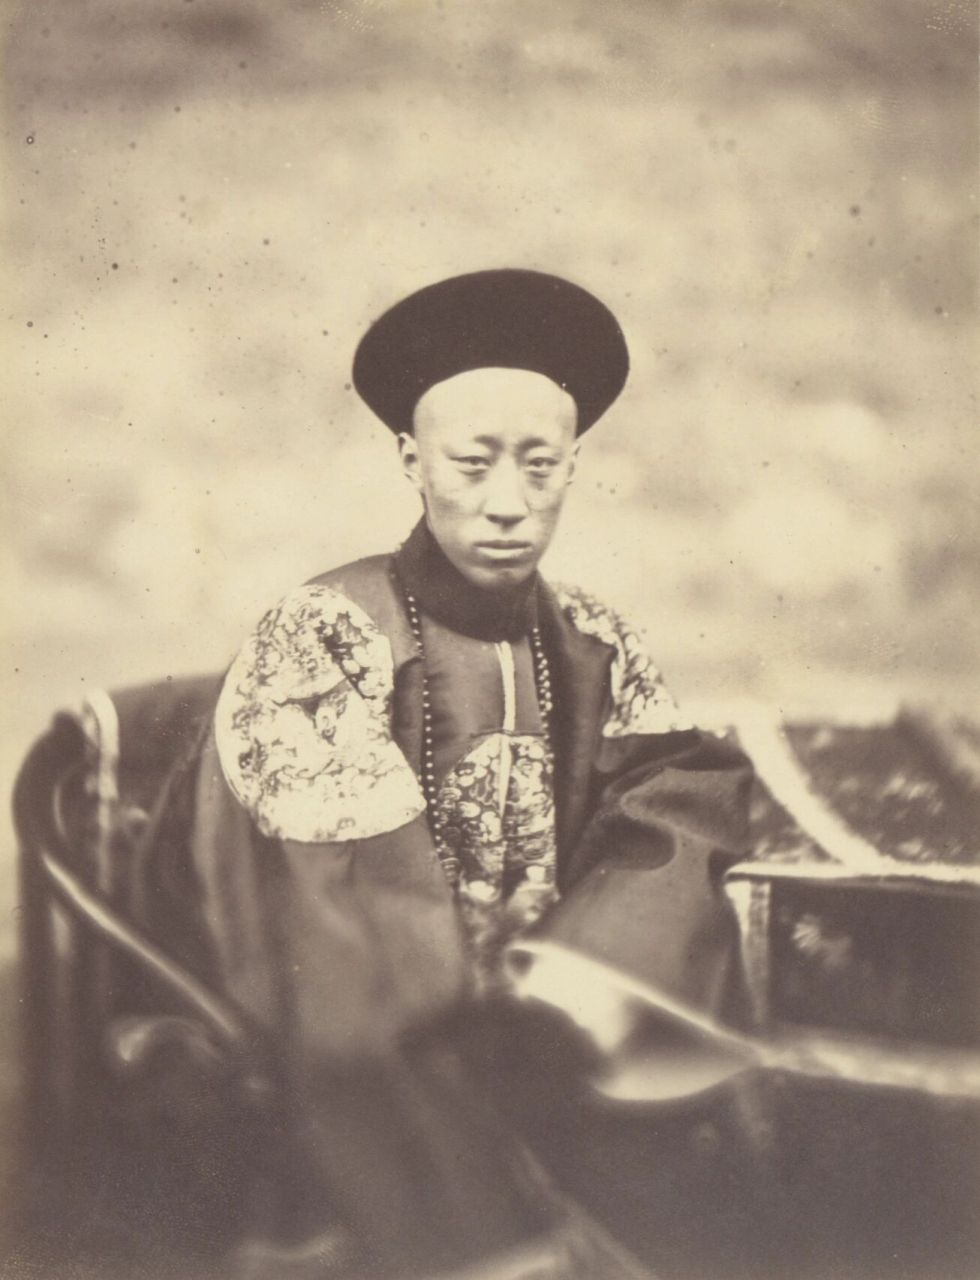
\includegraphics[width=0.7\linewidth]{Images/1}
\caption{恭亲王奕䜣(1833-1898)}
\label{fig:1}
\end{figure}

在恭亲王的支持推动下,1861年清政府通过在英国休假的海关总税务司李泰国(Horatio Nelson Lay),向英国订购了“中国”、“北京”、“江苏”等七艘西式明轮炮舰,这是近代中国迈出的通往蓝色世界的第一步(与此几乎同步,感受到太平天国军力压迫的江苏地方官员及上海本地士绅,也委托常胜军统领华尔的弟弟亨利·华尔(F.H.G.Ward)在美国购舰,分别命名“大清”、“江苏”、“浙江”,后值美国南北战争爆发,3舰被亨利·华尔擅自转售给美国北方政府,参加了南北战争)。血液里有着纳尔逊家族遗传的李泰国(李泰国的母亲是英国海军英雄纳尔逊的侄女),在英国政府默许下,将这次购舰活动看作是控制中国海上力量的机会,擅自委任英国海军上校阿思本(Sherard Osborn)为编队司令,舰队成员几乎全部雇佣英国人组成,并自作主张,单方面制订了绿底黄十字海军旗和舰队规章制度,规定舰队只服从中国皇帝和李泰国的命令,而且中国皇帝的命令必须在得到李泰国的认可后才能生效。这支全由英国人组成的中国舰队,几乎成了李泰国私人部队,史称李泰国舰队、阿思本舰队、吸血舰队等。7艘军舰远涉重洋抵达中国后,清政府对这支不受控制的舰队表现出了无论如何也不能接受的立场,经过反复争辩,最终一举将这支舰队拍卖遣散了事,由此,中国建设西式海军的第一次重要努力随着7舰的散去而破灭。

\begin{figure}[htbp]
\centering
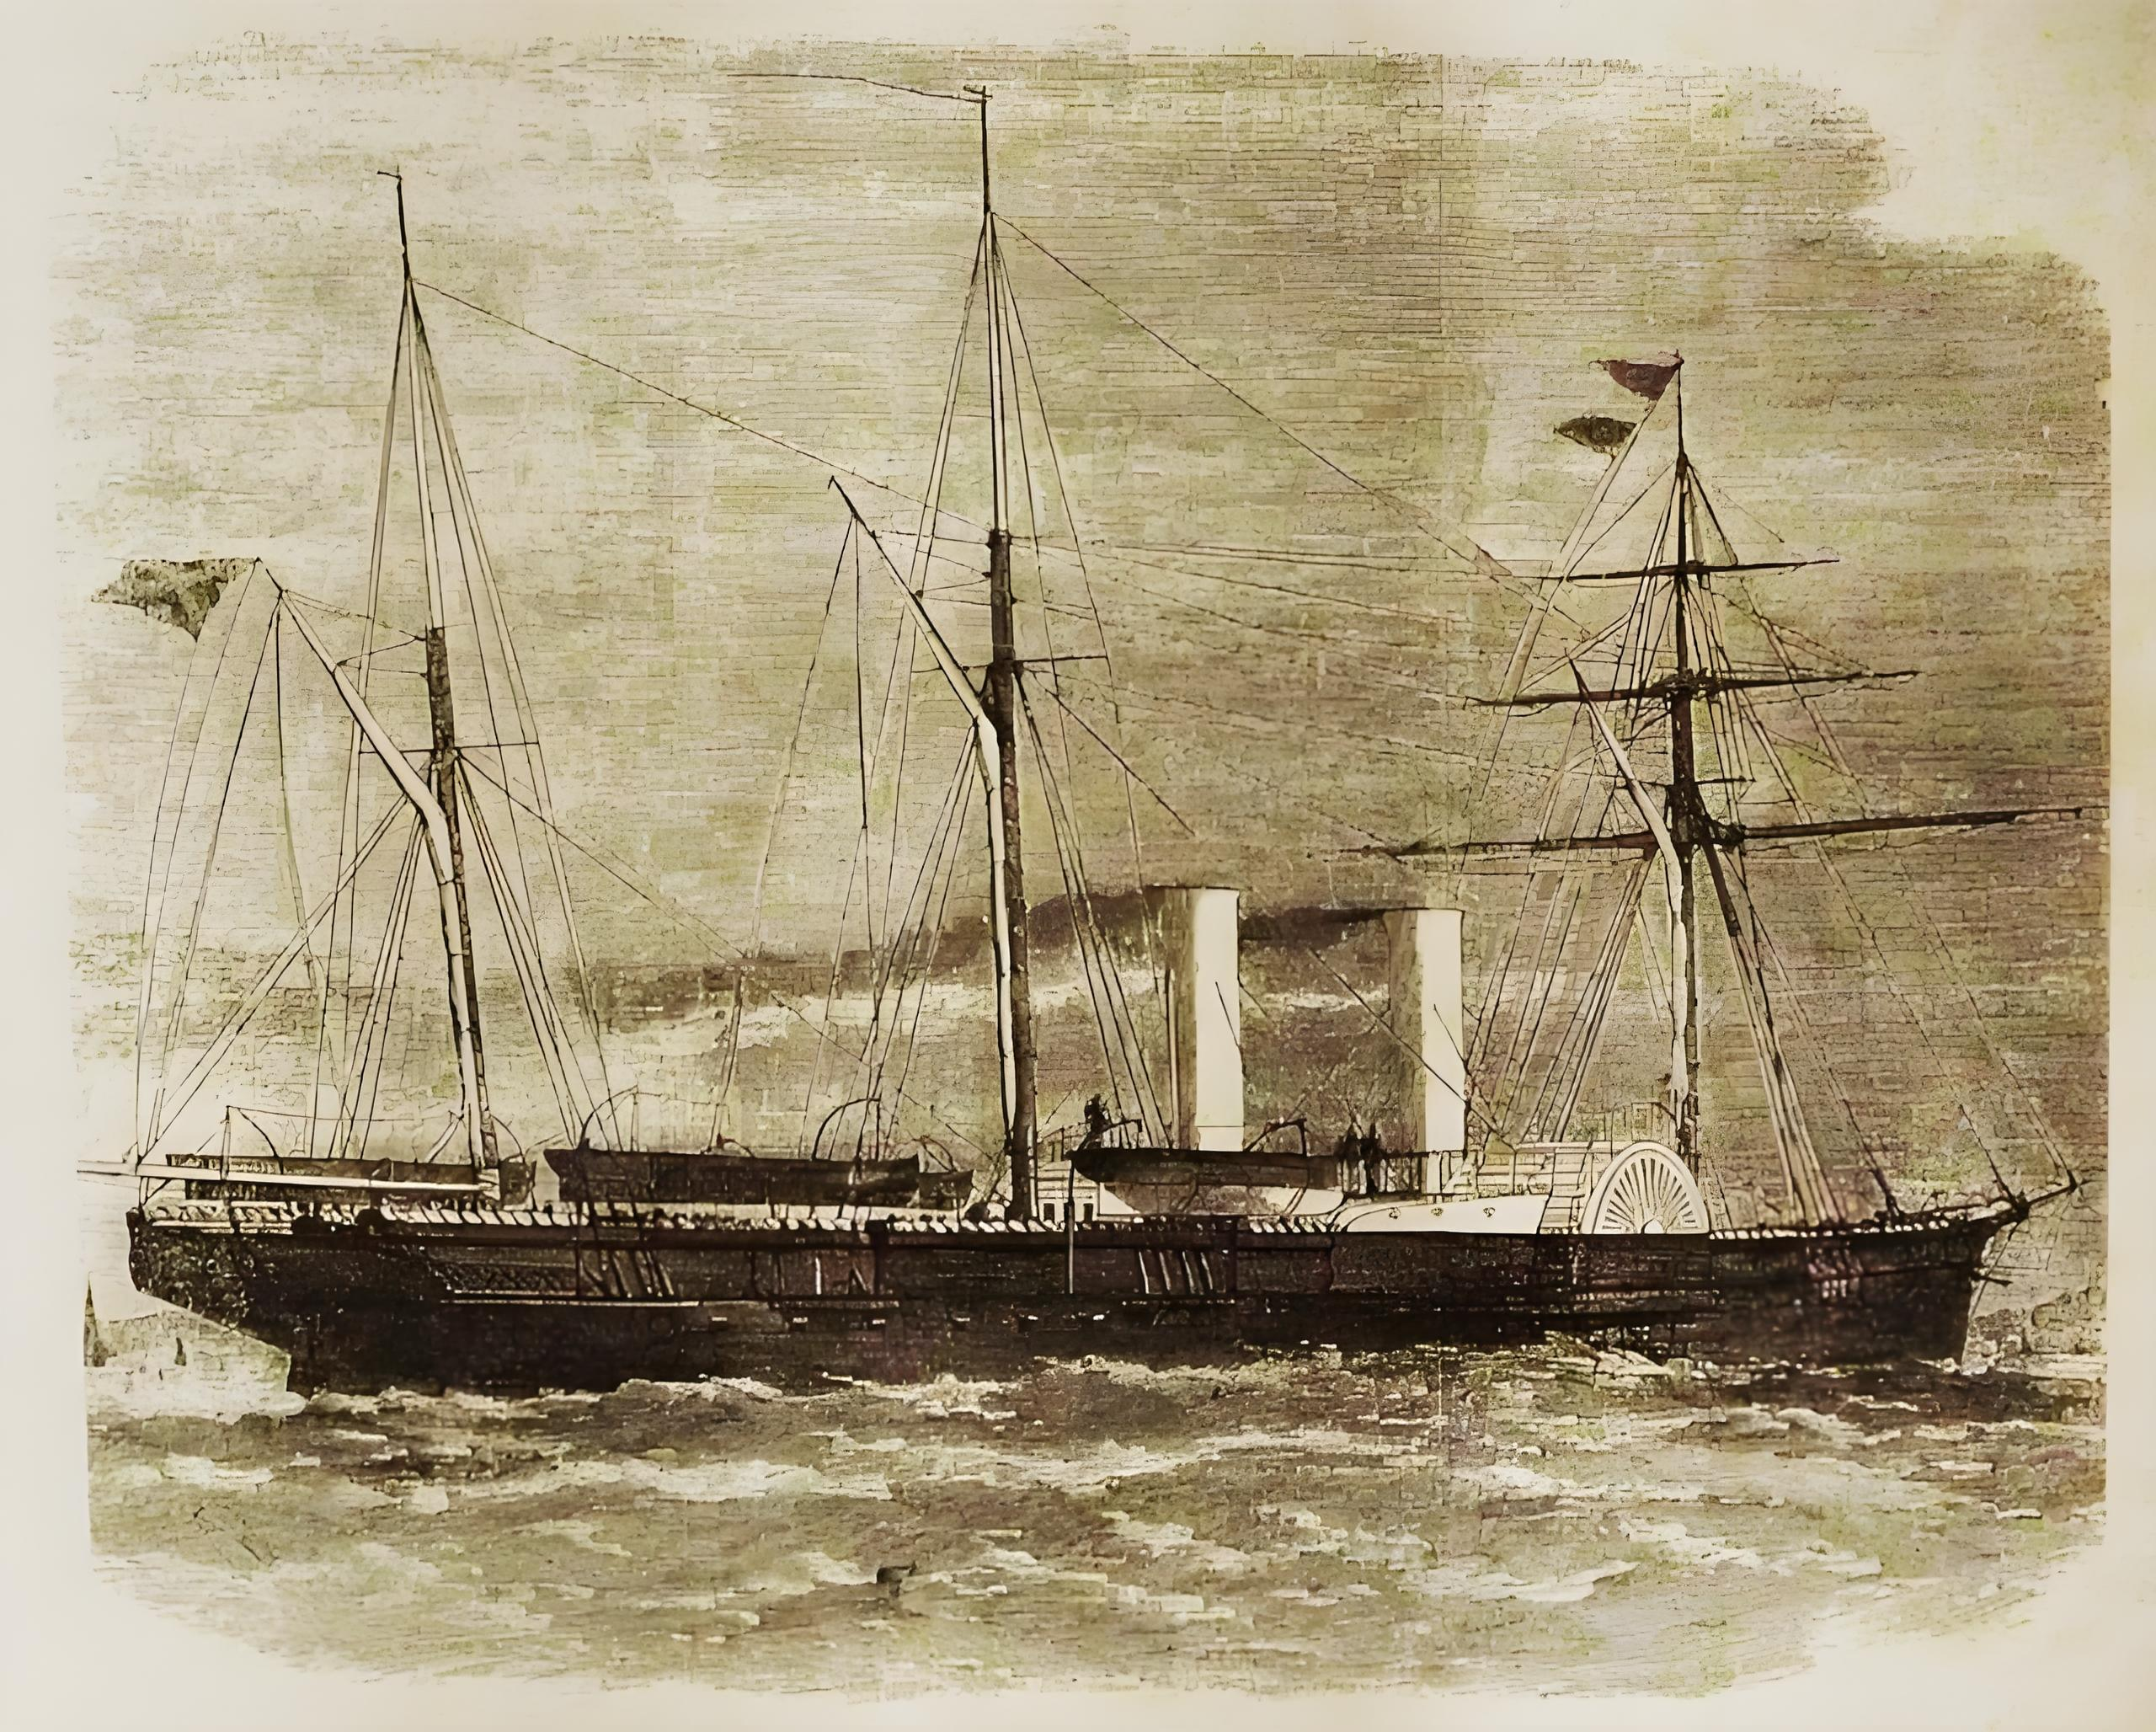
\includegraphics[width=1\linewidth]{Images/2}
\caption{西方铜版画:阿思本舰队的旗舰“江苏”号。海关总税务司李泰国组织的由英国人控制的中国舰队,给洋务官员上了教训深刻的一课,“权自我操”原则此后成为洋务活动的一条不容触碰的红线。}
\label{fig:1}
\end{figure}

令朝野上下极为难堪的阿思本舰队事件发生以后,中国国内“造舰”的呼声逐渐高涨,第一次出师就铩羽而归的教训,使得洋务派被迫更加谨慎地去对待一切与西方的交往事务,直接向西方获取军舰等武器,被认为是极易触及主权问题的敏感活动,就此很少有人愿意再涉足。此后,闽浙总督左宗棠、两江总督曾国藩先后在马尾、上海创建西式造船机构,开始了自力更生,自行建造近代化军舰的尝试。由于不可避免地受到技术起点低,专业人才匮乏,以及指导思想上存在误区等因素桎梏,这一阶段中国自行建造的军舰普遍存在舰型等级低等问题,大都属于炮舰和运输舰范畴,尚无法满足远洋作战的需求。

1871年,中国属国琉球的商船遭遇风暴漂流至福建省台湾岛,因言语不通,琉球船民与台湾土著发生争执,部分船民遭杀害。对于这一内政事件,清政府很快予以措置进行平息。但当时谁也未曾想到,与此毫无瓜葛的日本竟会借机生事。近代日本开始明治维新后,将对外扩张作为国策,为此整军经武,加强陆海军力量。1874年,借口要为琉球船民报仇,日本出兵大举入侵台湾,史称台湾事件。与此针锋相对,清王朝派船政大臣沈葆桢为钦差,赴台湾处置事变,船政水师舰船被纷纷调往,保障台湾海峡的交通、运输,以及与侵台日军抗衡、对峙。经过长时间相持,最终在列强调停下,这一事件草草收场。囿于当时海防力量薄弱,“明知彼之理曲,而苦于我之备虚……实以一经决裂,滨海沿江,处处皆应设防,各口之防难恃不得不以慎于发端\footnote{《同治十三年九月二十七日总理各国事务衙门奏》,中国近代史资料丛刊《洋务运动》1,上海:上海人民出版社1961年版,第26页。}”,担心事态扩大后无法应对,为尽早息事宁人,清王朝付出高昂的代价,除支付50万两银军费外,还被迫承认日本侵略台湾的举动是“保民义举”,实际上等于已经默认日本对中国、琉球藩属关系的挑衅,由此埋下了琉球亡国之祸的伏笔。

自三国时代以来,日本就被中国称为倭国,视为化外蛮夷,动辄对其嗤之以鼻,不以为然。然而,就是这个一贯被中华瞧不起的东邻小国,学习了一些西方先进技术后,竟然肆无忌惮向中国发起挑战,由此在中国社会引起的震动不啻于一声晴天霹雳。海防建设的重要性、紧迫性突现,而中国自造舰只存在的不足也暴露无遗。恭亲王奕䜣事后曾痛心疾首地在奏章中写道:“今日而始言备,诚病以迟;今日再不修备,则更不堪设想矣!”并追思自鸦片战争之后,中国尽管开展了建船厂、造军舰等旨在自强的事业,但“人人有自强之心,亦人人为自强之言,而迄今仍并无自强之实,从前情事几于日久相忘”\footnote{《同治十三年九月二十七日总理各国事务衙门奏》,中国近代史资料丛刊《洋务运动》1,上海:上海人民出版社1961年版,第26页。}。认为应当立刻抛开以往的成见,采取果断措施,尽快加强国家的海防实力。

“……查明一种快艇的吨位和造价,它的前甲板防护平台上要装载一门八十吨大炮,可在五百码外打穿二十英寸厚的钢板。问清最低必须吨位和优质货的最低价格。速复!询问保密!勿提中国!”\footnote{《赫致金第13号》,《中国海关密档》8,北京:中华书局1995年版,第20页。}

1874年10月23日,中日台湾事件交涉接近尾声之际,取代李泰国担任中国海关总税务司的赫德(Robert Hart),经由上海,向他在伦敦的忠实部下金登干(James Duncan Campbell)发去了上述这封电报。继夭折的阿思本舰队之后,清王朝第二次大规模外购军舰的活动渐渐拉开了帷幕,与第一次购舰活动用于镇压国内起义的目的不同,这次购舰主旨相当明确,就是巩固海防,抵御外侮。

\section{伦道尔式炮艇}

就在日本侵略台湾,中国朝野上下为之震惊、群情激愤的日子里,有个西方人的身影开始频繁地在总理衙门出没。身为英国在华利益的重要代言人,中国海关总税务司赫德敏锐地觉察到中国即将以日本为假想敌扩充海军的迹象。这位久居中国,深谙中国官场之道的英国人明白这将是影响未来中国海军事务的重要契机,良机不容错失,随即凭籍其特殊的身份,开始与总理衙门大臣恭亲王奕䜣密切接触,推销英国造军舰。自阿思本舰队事件之后,虽然左宗棠创立的船政福州马尾经历了近十年自造军舰的尝试,但日本竟然胆敢挑战中国,说明中国的海防实力并不见有多少起色,此时直接购买西方先进军舰的提议悄悄开始占据上风。

要加强海防,究竟应该以装备何种军舰为宜,围绕这一全新的命题,当时中国国内的官员大都是茫然无措,不知道从何做起。而喜欢夸夸其谈的赫德,本人实际对海军领域也只是略知皮毛,将中国人外购军舰的兴趣挑起后,赫德便急匆匆与远在伦敦的金登干商讨具体如何推销军舰。当时沈葆桢、李鸿章等中国官员从自己掌握的海军知识出发,急切想获取的是铁甲舰。但这种军舰造价过于昂贵,清政府一时无力负担,而且大型军舰对于操舰人员的专业技术知识也有极高的要求,遽难办理。很快,赫德和金登干都注意到了当时世界上一种最新潮的军舰,一种价格便宜,而且据说是大型铁甲舰天煞克星的小军舰。

\begin{figure}[htbp]
	\centering
	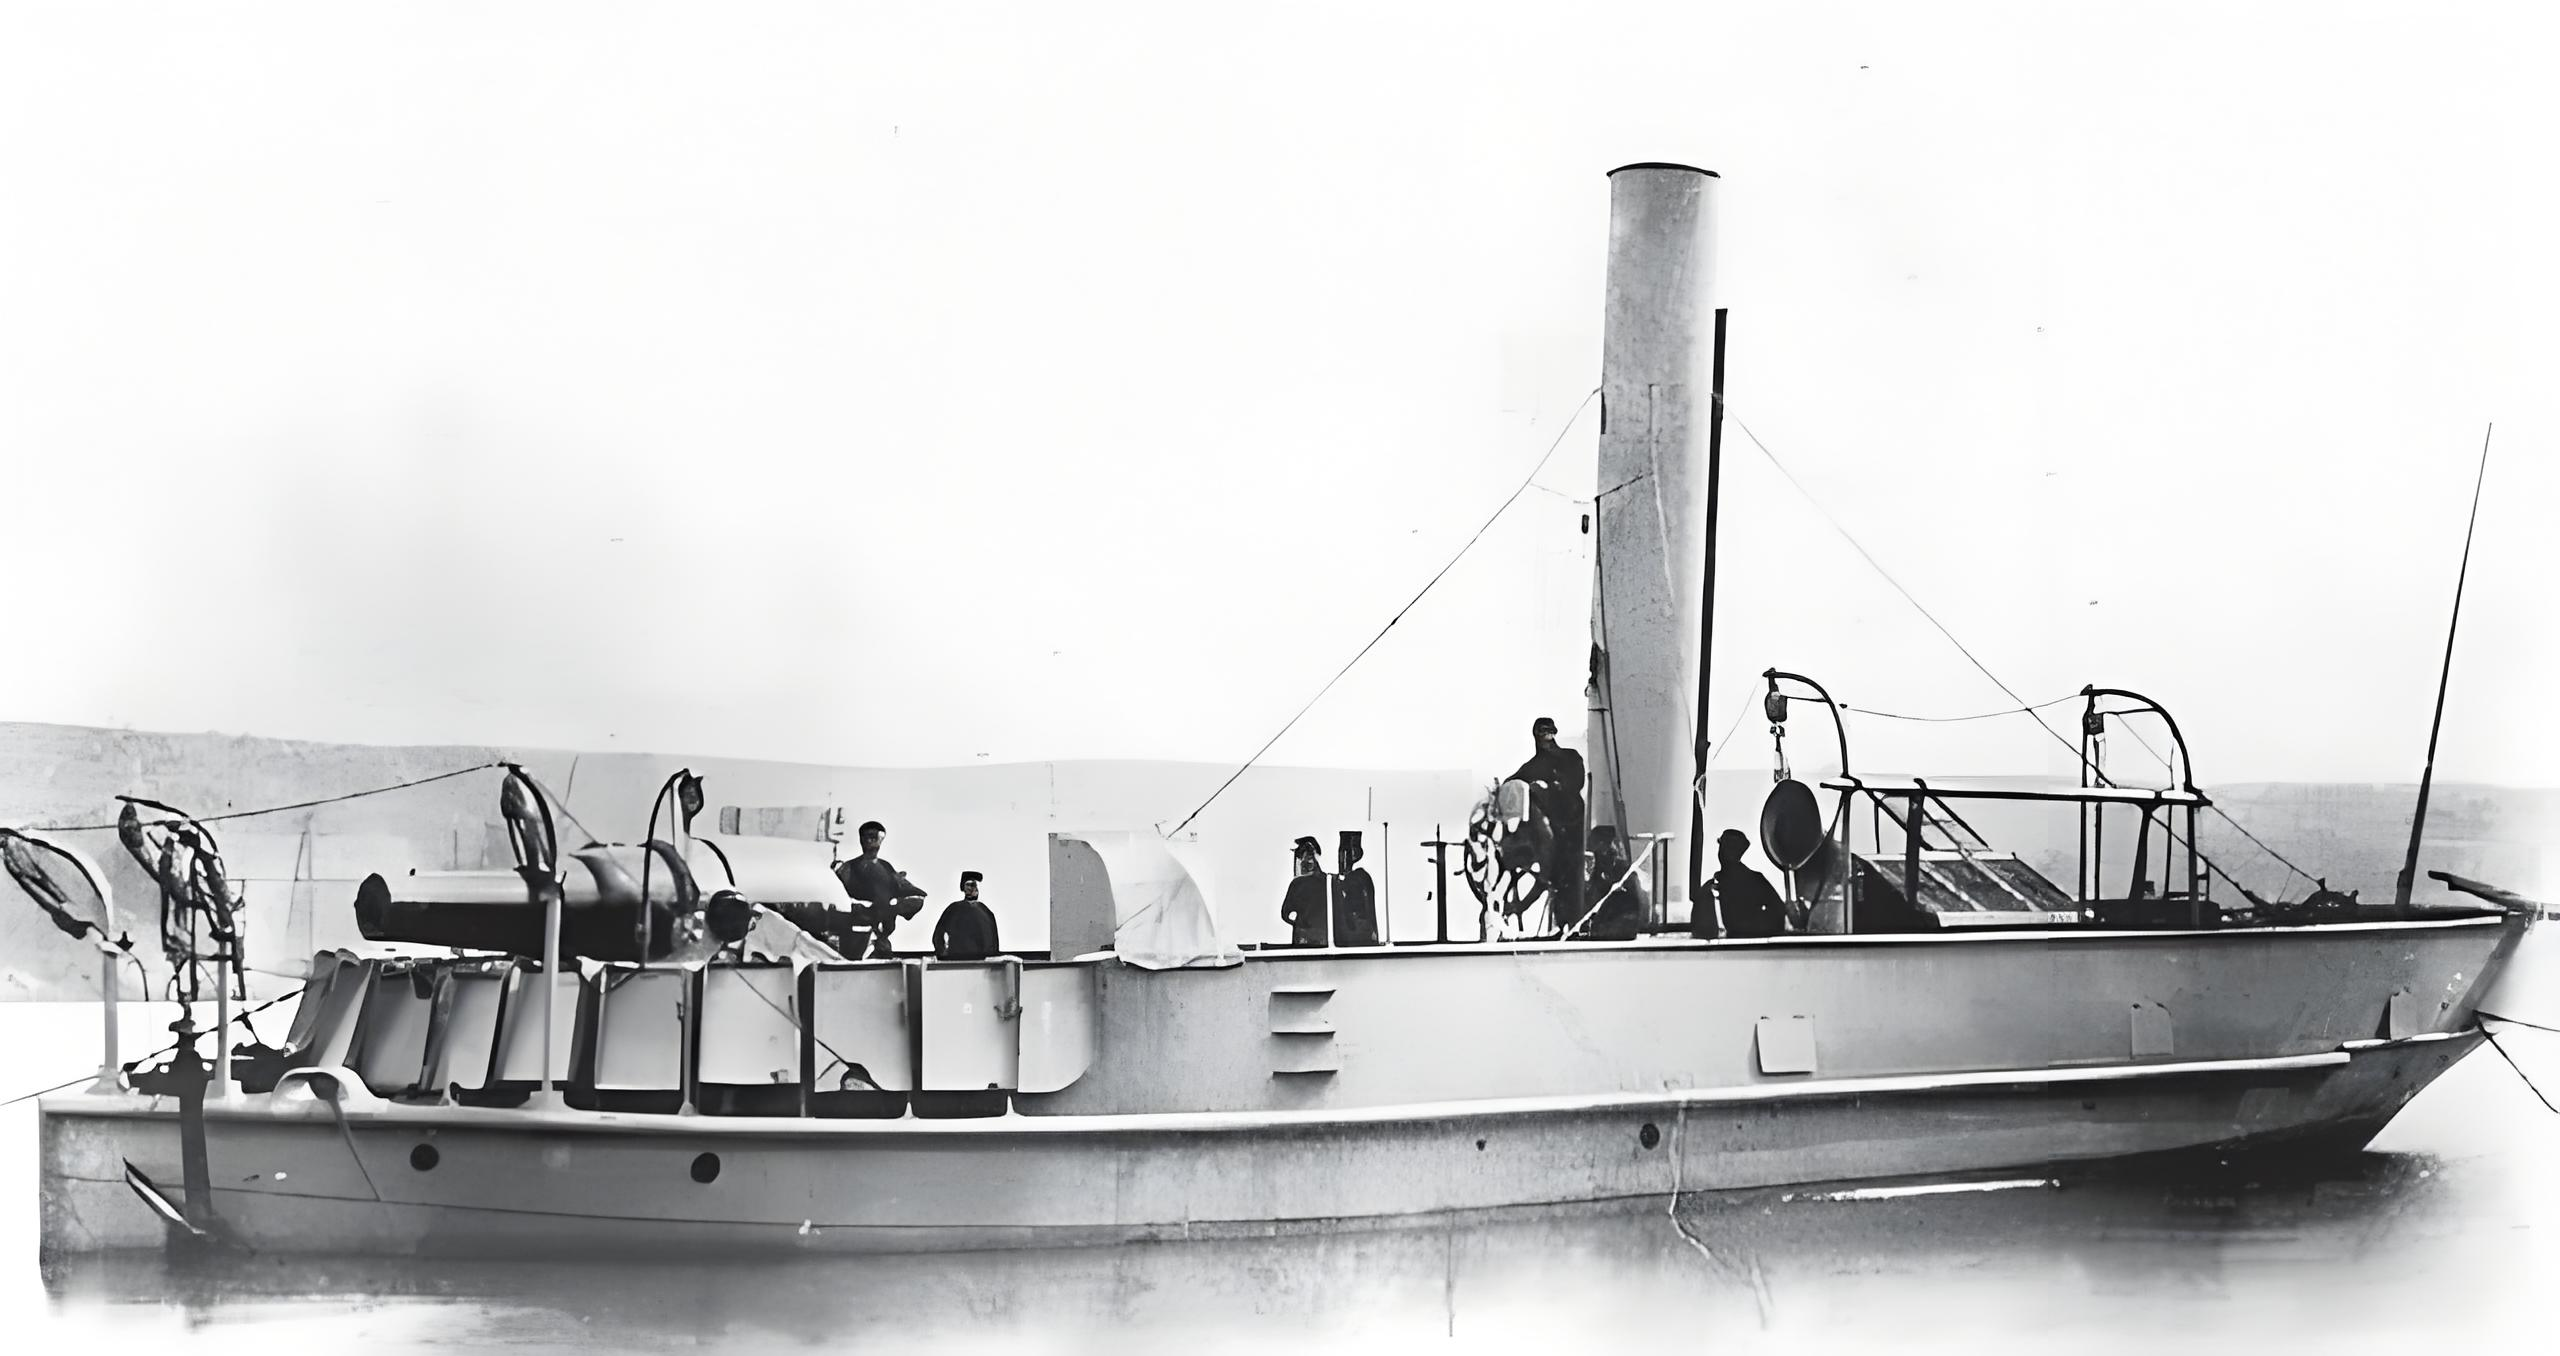
\includegraphics[width=1\linewidth]{Images/3}
	\caption{伦道尔的成名作、世界上第一艘蚊子船Staunch。依据浮动炮台的思想设计出来的这艘军舰,在当时的舰船之林中外形极为奇特,由于根本不考虑远海作战,这艘军舰完全抛弃了桅杆。}
	\label{fig:1}
\end{figure}

当中国东南马江之畔正在大兴土木建造福建船政船厂的时候,1867年12月4日,地球另一面的英国泰恩河(River Tyne)上,出现了一艘模样奇特的小军舰。在当时,连它的设计者乔治·伦道尔(George Wightwick Rendel)自己都没有想到,这艘小小的军舰竟然会成为他一生事业的重要奠基石。Staunch号,中国译为“师丹”炮船,是英国劳沃克船厂(Low Walker)建造的排水量仅有180吨的小型炮艇,长度24.38米,宽7.6米,显得短而宽,吃水1.97米,装备有2台蒸汽机、2座锅炉,主机功率150马力,航速7节。和进入蒸汽时代以来那种比巡洋舰小,航速迟缓,在甲板两侧安放火炮,“以供杂役”的旧式炮船完全不同,这艘小炮船具有几个非常鲜明的特征。它彻底抛弃了传统的船旁列炮布置法,而是在船头露天安装了一门9英寸口径的前装线膛炮,巨炮的炮身安装在一套带有4个支柱的地井式炮架上,整个系统异常复杂。平时火炮低座在船体里,以防重心过高,保持军舰的稳性,使用时则通过液压系统,在4至6分钟内将火炮举升到甲板上,每发射1发之后,火炮在自身巨大的后坐力推动下,再缓缓降到甲板下,进行下一次射击的装填工作。显得古怪的是,这种军舰在火炮发射前必须下锚,否则谁也无法预料巨大的后坐力会对小船产生怎样的影响。\footnote{Peter Brook: Warshipsfor Export-Armstrong Warships1867--1927,1999,p24.David Lyon、RifWinfield: All The Ships of The Royal Navy1815--1889,Chatham Publishing 2004,p279.Conway's All The World's Fighting Ships 1860--1905,Conway Maritime Press 1979,p111.}

除去独特的船头大炮布置方法,这艘小军舰的外形也颇具特色,舰艏有一段锚甲板,采用的是破浪效果较好的龟甲样式,上面安装有吊锚杆等设备。锚甲板向后的主甲板部分,四面都围有用于保护舰员的围壁。在船艏安装有火炮的甲板周围则装有更高的可折倒的围壁,用于防止军舰在高速航行时,海浪扑进火炮甲板。军舰的主炮炮管通过这道围壁前方一个很小的炮门开口向外伸出,因为炮门横向空隙很小,主炮几乎不能左右转动,必须采用整船瞄准法,即通过军舰的自身转动,来实现调整火炮的横向射击角度。为此,伦道尔将这艘小军舰的操舵系统设计得极为灵便,转舵速度较一般军舰为高,仅用2分45秒全船就可以旋转一圈。在接近主甲板中部的位置上,矗立着高高的烟囱,让当时的造船界为之惊讶的是,这艘小船竟然连一根桅杆都没有,而且在这艘船上除了舰长室外,甚至没有为舰员留出任何居住空间。浅眼来看,这些设计,不光是无法远距离航行,甚至连如何悬挂航海信号旗帜都成了问题。其实伦道尔赋予这种军舰独特的设计思路就在这里得到了最好的诠释。即,这种短宽的小型军舰根本就不是用来出海作战的。

\begin{figure}[htbp]
	\centering
	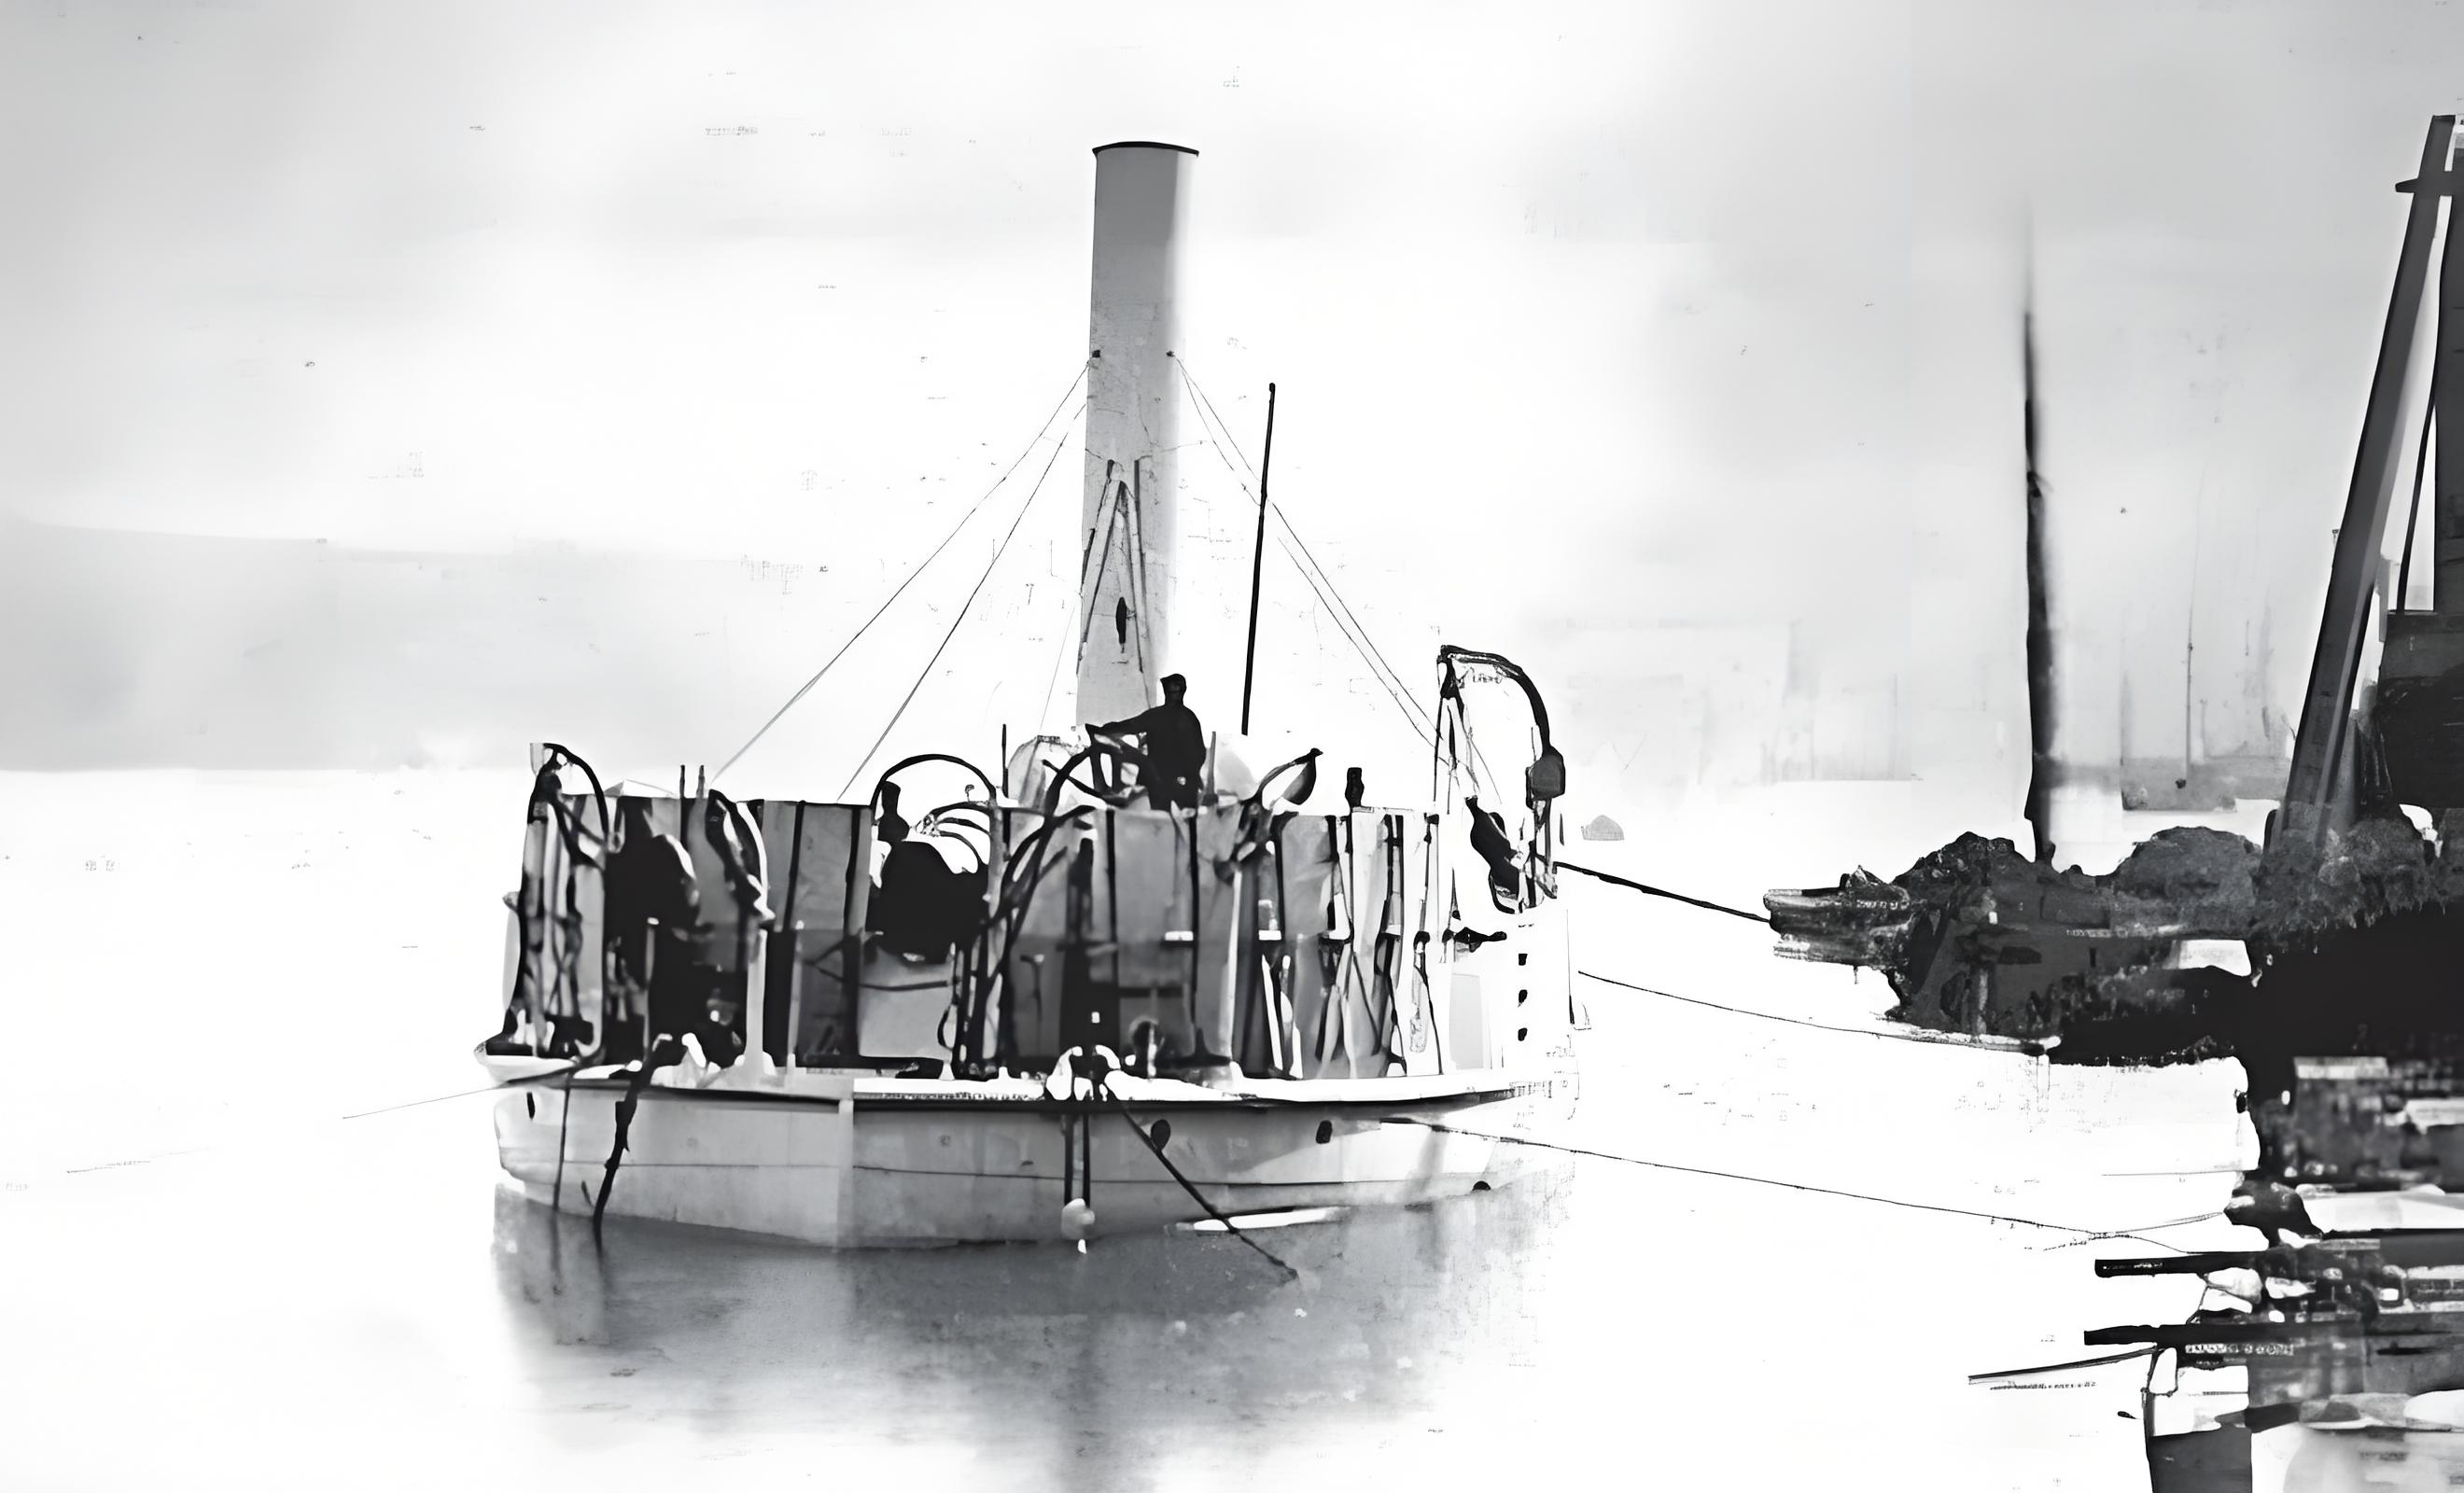
\includegraphics[width=1\linewidth]{Images/4}
	\caption{Staunch号的另一张照片,此时船艏防浪围壁是竖起状态。}
	\label{fig:1}
\end{figure}

19世纪中期的世界,大口径火炮是最具威势的兵器。在海洋上,它的搭载平台是大型铁甲舰,陆地上,则是坚固的炮台工事。结果铁甲舰和炮台发展成了一对相生相克的冤家,相对于铁甲舰,炮台上黑洞洞的巨炮阴森可怖,难以冒犯,而炮台由于是固定的建筑,万一铁甲舰不进入自己的防守范围,而是另辟蹊径,暗渡陈仓,炮台就成为虚设。为解决这一对矛盾,当时各国的陆海军界都绞尽脑汁,结果往往落入无限增大火炮口径、威力的套路中。

\begin{figure}[htbp]
	\centering
	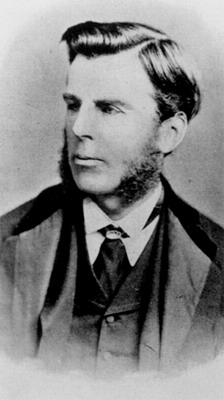
\includegraphics[width=0.5\linewidth]{Images/5}
	\caption{乔治·伦道尔,英国近代著名舰船设计师,因开创了蚊子船这一独特的舰船样式而闻名,此后他又创造了具有开创性的军舰——“超勇”级撞击巡洋舰,与近代中国海军的渊源颇深。}
	\label{fig:1}
\end{figure}

伦道尔的Staunch创造了一种全新的武器——“水炮台”,即水上的炮台,外形看上去是艘船,实则并不作为军舰来使用,搭载巨炮的小船只不过是大炮的安装平台而已。水炮台和同样装备大口径火炮的铁甲舰相比,造价上可谓有着天壤之别,但装载的火炮所具有的威力却并无太大不同,属于低成本、极具性价比的火炮搭载平台。虽然不能到大海上与铁甲舰争雄,但是它搭载的火炮同样可以给铁甲舰以巨大的威慑,近海防御时占有优势。而相对于耗费大量土木人工,经年累月才能构筑起来的陆地炮台,水炮台在价格低廉的优势之外,还有一个更大的优势,就是这种“炮台”能够移动。可以根据实际情况,临时大量布置到需要加强的濒海地域,“驻扼口隘其力能拒甲舰”,短时间内即能构成一个海上的炮台群。

这种名为炮船Gunboat,实则是炮台的军舰,在当时中国被翻译为“根驳”船、“根婆子”,又根据其特征称为“蚊子船”,意指这种军舰虽然体格小巧,不过万一被叮上一口,也不是好受的事。在西方,这种军舰则根据设计师的名字称为伦道尔式炮艇。它一经诞生,立刻引起轰动,被认为是用于要港防御的最新利器,英国皇家海军前后共购进了数十艘,其他一些海军国家也都大感兴趣,纷纷解囊采购,设计师伦道尔由此名扬四海。

1874年发给金登干的电报中,赫德所询问的“快艇”正是这种伦道尔式炮艇。赫德深知当时清王朝的财政情况捉襟见肘,与其推销短时间内中国根本没能力购买的大型铁甲舰,不如推销这种价格低廉,而且据称能打败铁甲舰的小型炮艇——蚊子船。同时,英国人并不希望中国拥有一支具有远洋作战实力的真正海军,他们所愿意看到的仅仅是中国能维持一支小规模的近海巡缉力量,能够自行绥靖海面,对付盗匪就已经足够。

今天值得重新审视的是,尽管赫德、金登干为推销军舰不遗余力,大肆宣传,但赫德对蚊子船的用途其实有清醒的认识,称这种船只是在浅水区对付铁甲舰的利器。对这一点,李鸿章也予以认同,认为“有此巨炮小船,守口最为得力,较陆地炮台更为灵活”。至于后来金登干等夸夸其谈,越说越奇,宣称这种军舰能在波涛汹涌的大海上作战,则纯属其一贯说话夸张的浮夸作风,实际李鸿章、赫德等从一开始就已经明了,这型军舰就是一种水上炮台。而后来很多对舰船知识一无所知的言官文人,以李鸿章买回来的蚊子船并不能出海作战为由,认为这种船是西方生产的劣质货,是专门设计用来诈骗中国的,则多少有些不辨菽麦的嫌疑。实际情况是,针对所谓蚊子船可以出海作战的荒谬说法,李鸿章根本不为所惑,而且在南洋大臣沈葆桢的催促下,私下已在打探丹麦、美国等国出售二手铁甲舰的信息。

1875年春天,经过向阿姆斯特朗公司询价,赫德正式将舰型方案提交给总理衙门,对这种新潮事务拿捏不稳的恭亲王则击鼓传花,将具体洽谈、购办的责任转交给北洋大臣李鸿章。从太平天国战争时代,就开始和西方人打交道,并在自己的军队中大量采用西式武器的李鸿章,是当时中国官场少有的善于处理外交事务的高层官僚,而且又身负京畿防务重责,选择他来办理新潮的海军,在恭亲王看来是再适合不过的人选。作为这一决策的继续,不久之后一道谕旨降到李鸿章面前:“著派李鸿章督办北洋海防事宜……所有分洋分任练军设局及招致海岛华人诸议,统归该大臣等择要筹办”\footnote{《光绪朝上谕档》1,桂林:广西师范大学出版社1996年版,第108页。},从此李鸿章成了中国北方海防建设的主管官员。

得到恭亲王授意,赫德奔赴北洋大臣驻地天津,上门咨商推介蚊子船。最后摆在李鸿章面前的,分别是装备80吨、38吨、26.5吨前膛火炮的三种方案。精明老道的李鸿章并没有立刻表态,而是四处咨询关于这些军舰的各种情况,并私下通过法国公使以及江海关直接获取国外市场行情,以做参照对比。咨询过程中,李鸿章突然发现一个问题:“查西人论炮不计身重,先问口径若干寸”,即按照海军专业用语,谈论火炮的类别一般都是说火炮口径而没有拿火炮的重量作为类别区分标志的,李鸿章似乎是觉察到了一点什么。\footnote{《复议购办枪炮铁船》,《李鸿章全集》31,合肥:安徽教育出版社2008年版,第140页。}赫德、金登干顿时显得颇为狼狈,急忙设法补充了相关参数。经过完善后的资料可见,当时提出的备选方案分别是:排水量1300吨,装备16英寸口径火炮,报价93000英镑,合279000两银;排水量440吨,装备12.5英寸口径火炮,报价33400英镑,合100200两银;排水量320吨,装备11英寸口径火炮,报价23000英镑,合69000两银;排水量260吨,装备9英寸口径火炮,报价20000英镑,合60000两银。\footnote{《赫总税司面译金登干来函》,《李鸿章全集》31,合肥:安徽教育出版社2008年版,第197-198页。}

经过一番权衡,李鸿章致函总理衙门,表示对恭亲王创办西式海军决心的感佩,从造价、可信度等角度出发,将备选的几家外国洋行全部否决,支持恭亲王通过赫德购买军舰的想法,认为“总税司经办当较洋行可靠”。随后,便与赫德进行仔细会商,认为备选方案中排水量260吨、装备9英寸口径火炮的型号,其火炮的威力和船只吨位都过小,意义不大。排水量1300吨,装备16英寸口径巨炮的舰型,吃水过深,且火炮口径太大,“为泰西向未有之巨炮”,担心这种从来没有使用前例的火炮不够可靠,不甘心为试验这种火炮买单,于是将这两个方案予以舍却。决定订购装备12.5英寸和11英寸口径火炮的蚊子船各1艘,旋又因各订1艘过于单薄,改为各订造2艘,同时约定,未来如得到16英寸口径巨炮使用可靠的消息,可以考虑再订购1艘装备16英寸口径火炮的大型蚊子船。\footnote{《致总署议购船炮》,《李鸿章全集》31,合肥:安徽教育出版社2008年版,第202-203页。}

4艘蚊子船由中国海关经手代办,向英国著名的火炮生产商阿姆斯特朗公司(Armstrong)订造,为预防阿思本舰队事件重演,1875年4月,李鸿章与赫德仔细订立了购舰合同,除了用大量文字就军舰的型号、质量、验收条款进行详细规定外,合同中载明,将来帮助驾驶军舰到中国的英国水手,在交接完毕后必须立刻离开中国。根据合同,装备11英寸火炮的蚊子船造价23000英镑,装备12英寸火炮的蚊子船造价33400英镑,分别折合中国银76659两和111322两,外加运费65940两,总计合同金额45万两银。按照阿姆斯特朗公司的惯例,合同签订后先付1/3,军舰造成一半后再付1/3,全成后付剩余部分。\footnote{《与赫总税司议定购办船炮章程》,《李鸿章全集》31,合肥:安徽教育出版社2008年版,第198页。}由恭亲王奏请,清政府批准合同,并对购舰经费做出布置,从江汉、九江、江海、浙海、粤海5口的海关关税内提取。\footnote{《光绪元年四月初二日总理各国事务衙门奕訢等奏折附片》,中国近代史资料丛刊《洋务运动》2,上海:上海人民出版社1961年版,第335-336页。}

1875年6月22日,赫德致电金登干,通知他中国购买4艘蚊子船的首付已经汇至专门的账户,要求立即准备合同草案、规格书、蓝图,迅速开工,“已去公文授权你从阿姆斯特朗厂购买四艘战舰,两艘载二十六吨大炮,两艘载三十八吨大炮,钱已交银行。”近代中国第二轮大规模的外购军舰活动正式开始。\footnote{《赫致金第10号》,《中国海关密档》8,北京:中华书局1995年版,第45页。}

\section{“龙骧”“虎威”;“飞霆”“策电”}

出于对自己第一次经手购舰的慎重,赫德在向金登干下达购买军舰指令的电文中,特别强调了军舰的质量。不久后,金登干便与阿姆斯特朗公司签订合同,规定11英寸口径大炮的蚊子船要在8个月内建成,装备12英寸口径炮的蚊子船限期13个月建成。\footnote{《金致赫第47号》,《中国海关密档》8,北京:中华书局1995年版,第53-54页。}4艘军舰的火炮由阿姆斯特朗公司制造,军舰的舰体部分转包给泰恩河畔纽卡斯尔(Newcastle)的米切尔船厂(Mitchell)建造。很快,4艘新潮军舰在英国的船台上陆续开工了,金登干为方便起见,用希腊文字母分别将她们命名为“阿尔法”、“贝塔”、“伽马”、“戴而塔”(Alpha、Beta、Gamma、Delta),因为这种独特的命名方式,中国蚊子船在西方又有个别号:字母炮艇。

其中“阿尔法”、“贝塔”属于装备11英寸口径火炮的一级,1875年9月21日同时开工,工厂建造编号327、328。舰体完全铁质,整体布局和蚊子船的开创之作Staunch非常相像。军舰排水量320吨,舰长35.97米,宽8.23米,吃水2.29米,动力系统为2台汤普森公司(Thompson)造蒸汽机、2台燃煤锅炉,主机功率235马力,双轴推进,航速10节,煤舱标准载煤40吨,最大载煤50吨。为保证军舰达到设计标准的机动性,军舰艏艉水下的线型完全一样,而且都安装有舵叶。\footnote{Conway's All The World's Fighting Ships 1860-1905,Conway Maritime Press 1979,p399.Peter Brook:Warships for Export-Armstrong Warships 1867-1927,1999,p30.}

这级军舰的主要武器便是安装在船头的阿姆斯特朗11英寸口径2号前膛炮,属于从炮口装填的前装线膛炮,火炮实际口径279.4毫米,炮管长4318毫米,药膛长660毫米,炮管内壁有9根来复线,每根长3023毫米,火炮可以使用3种炮弹,实心弹与开花弹均重249千克,霰弹重242千克,药包重38.5千克,在274米距离上测得能击穿326毫米厚的装甲。\footnote{《各国水师炮表·英国》,许景澄:《外国师船图表》,柏林使署光绪十二年石印版,卷十一。}火炮前方的甲板下,有一套复杂的液压弹药提升、装填装置,装填时,需将火炮的炮口低俯,以便弹药从前下方装入炮膛。此外,军舰主甲板中后部两侧还各装备有1门3英寸口径的阿姆斯特朗后膛舢板炮,另外还装备有1门作为近卫武器的格林机关炮。

\begin{figure}[htbp]
	\centering
	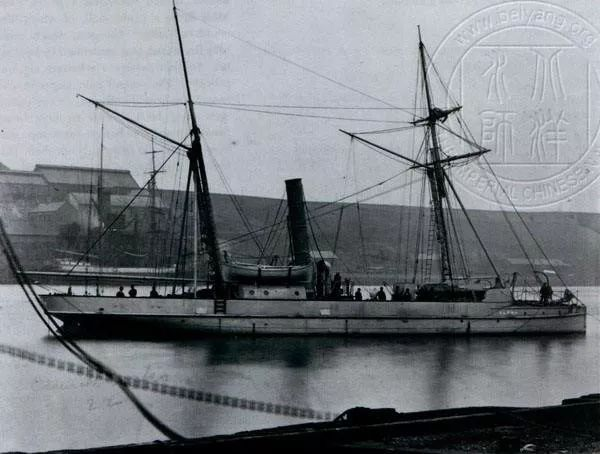
\includegraphics[width=1\linewidth]{Images/6}
	\caption{在泰恩河上进行航试的“阿尔法”(“龙骧”)舰,军舰舰艏前部的舷侧可以清楚看到临时油漆的英文舰名Alpha。和蚊子船的开山之祖Staunch外观上最明显的区别就是增加的两根桅杆。}
	\label{fig:1}
\end{figure}

相比起蚊子船的开山之作Staunch号,“阿尔法”在舰体外形上又创造了很多独特设计,考虑到这型军舰需要远涉重洋返回中国,在最初的设计上添加了2根桅杆以便挂帆,为增加强度,两根桅杆还各有人字型的副杆支撑,“阿尔法”级成了独特的带帆蚊子船。此外,“阿尔法”级主炮炮位前部外侧的装甲围壁为不能折倒的固定样式,厚度0.5英寸,具有有限的防弹片能力。在主炮之后不远,有一块对前左右三面防护,厚度同为0.5英寸的装甲挡板,作战时,指挥人员可以站在挡板之后,算是一个后部敞开式的装甲司令塔。在军舰主甲板中部的烟囱附近,设有一个位置较高视野开阔的露天指挥台,安装有舵轮、罗经、车钟等航海设备。

“伽马”、“戴而塔”是装备12英寸火炮的那级,1875年12月27日同时开工,建造编号334、335。舰体也是铁质,体形比“阿尔法”略大,排水量提升到420吨,舰长36.58米,宽9.14米,吃水2.44米,动力系统是2座汤普森公司造蒸汽机,1座燃煤锅炉,双轴推进,主机功率270马力,航速9节,煤舱正常容量50吨,最大容量60吨,军舰同样采用了艏艉舵叶。\footnote{Conway's All The World's Fighting Ships 1860-1905,Conway Maritime Press 1979,p399.Peter Brook:Warships for Export-Armstrong Warships 1867-1927,1999,p30.}主炮选用1门阿姆斯特朗12.5英寸口径1号前膛炮,也属于前装线膛炮,实际口径317.5毫米,炮身长5727毫米,药膛长699毫米,炮膛内有9根长度4330毫米的来复线,火炮同样使用3种炮弹,371千克重的实心弹、375千克重开花弹,以及373千克重霰弹,药包重72.6公斤,274米距离上测得穿甲能力414毫米,火炮的弹药提升及装填方式与“阿尔法”级相同。\footnote{许景澄,《外国师船图表》,柏林使署光绪十二年石印版,卷十一,第1-2页。}此外,“伽马”级在军舰主甲板中部还装有2门阿姆斯特朗2.75英寸口径后膛舢板炮,和1门格林机关炮。同样,考虑到回国将要经历的长距离航行,蚊子船有限的载煤难以供应,也增加了2根桅杆的全帆装设计。这级军舰从外观上整体看来,与“阿尔法”级非常相似,但是主炮周围的围壁遮护范围更大,而且主炮后方设有碉堡状的封闭式司令塔,防护方面比“阿尔法”有所改进。

\begin{figure}[htbp]
	\centering
	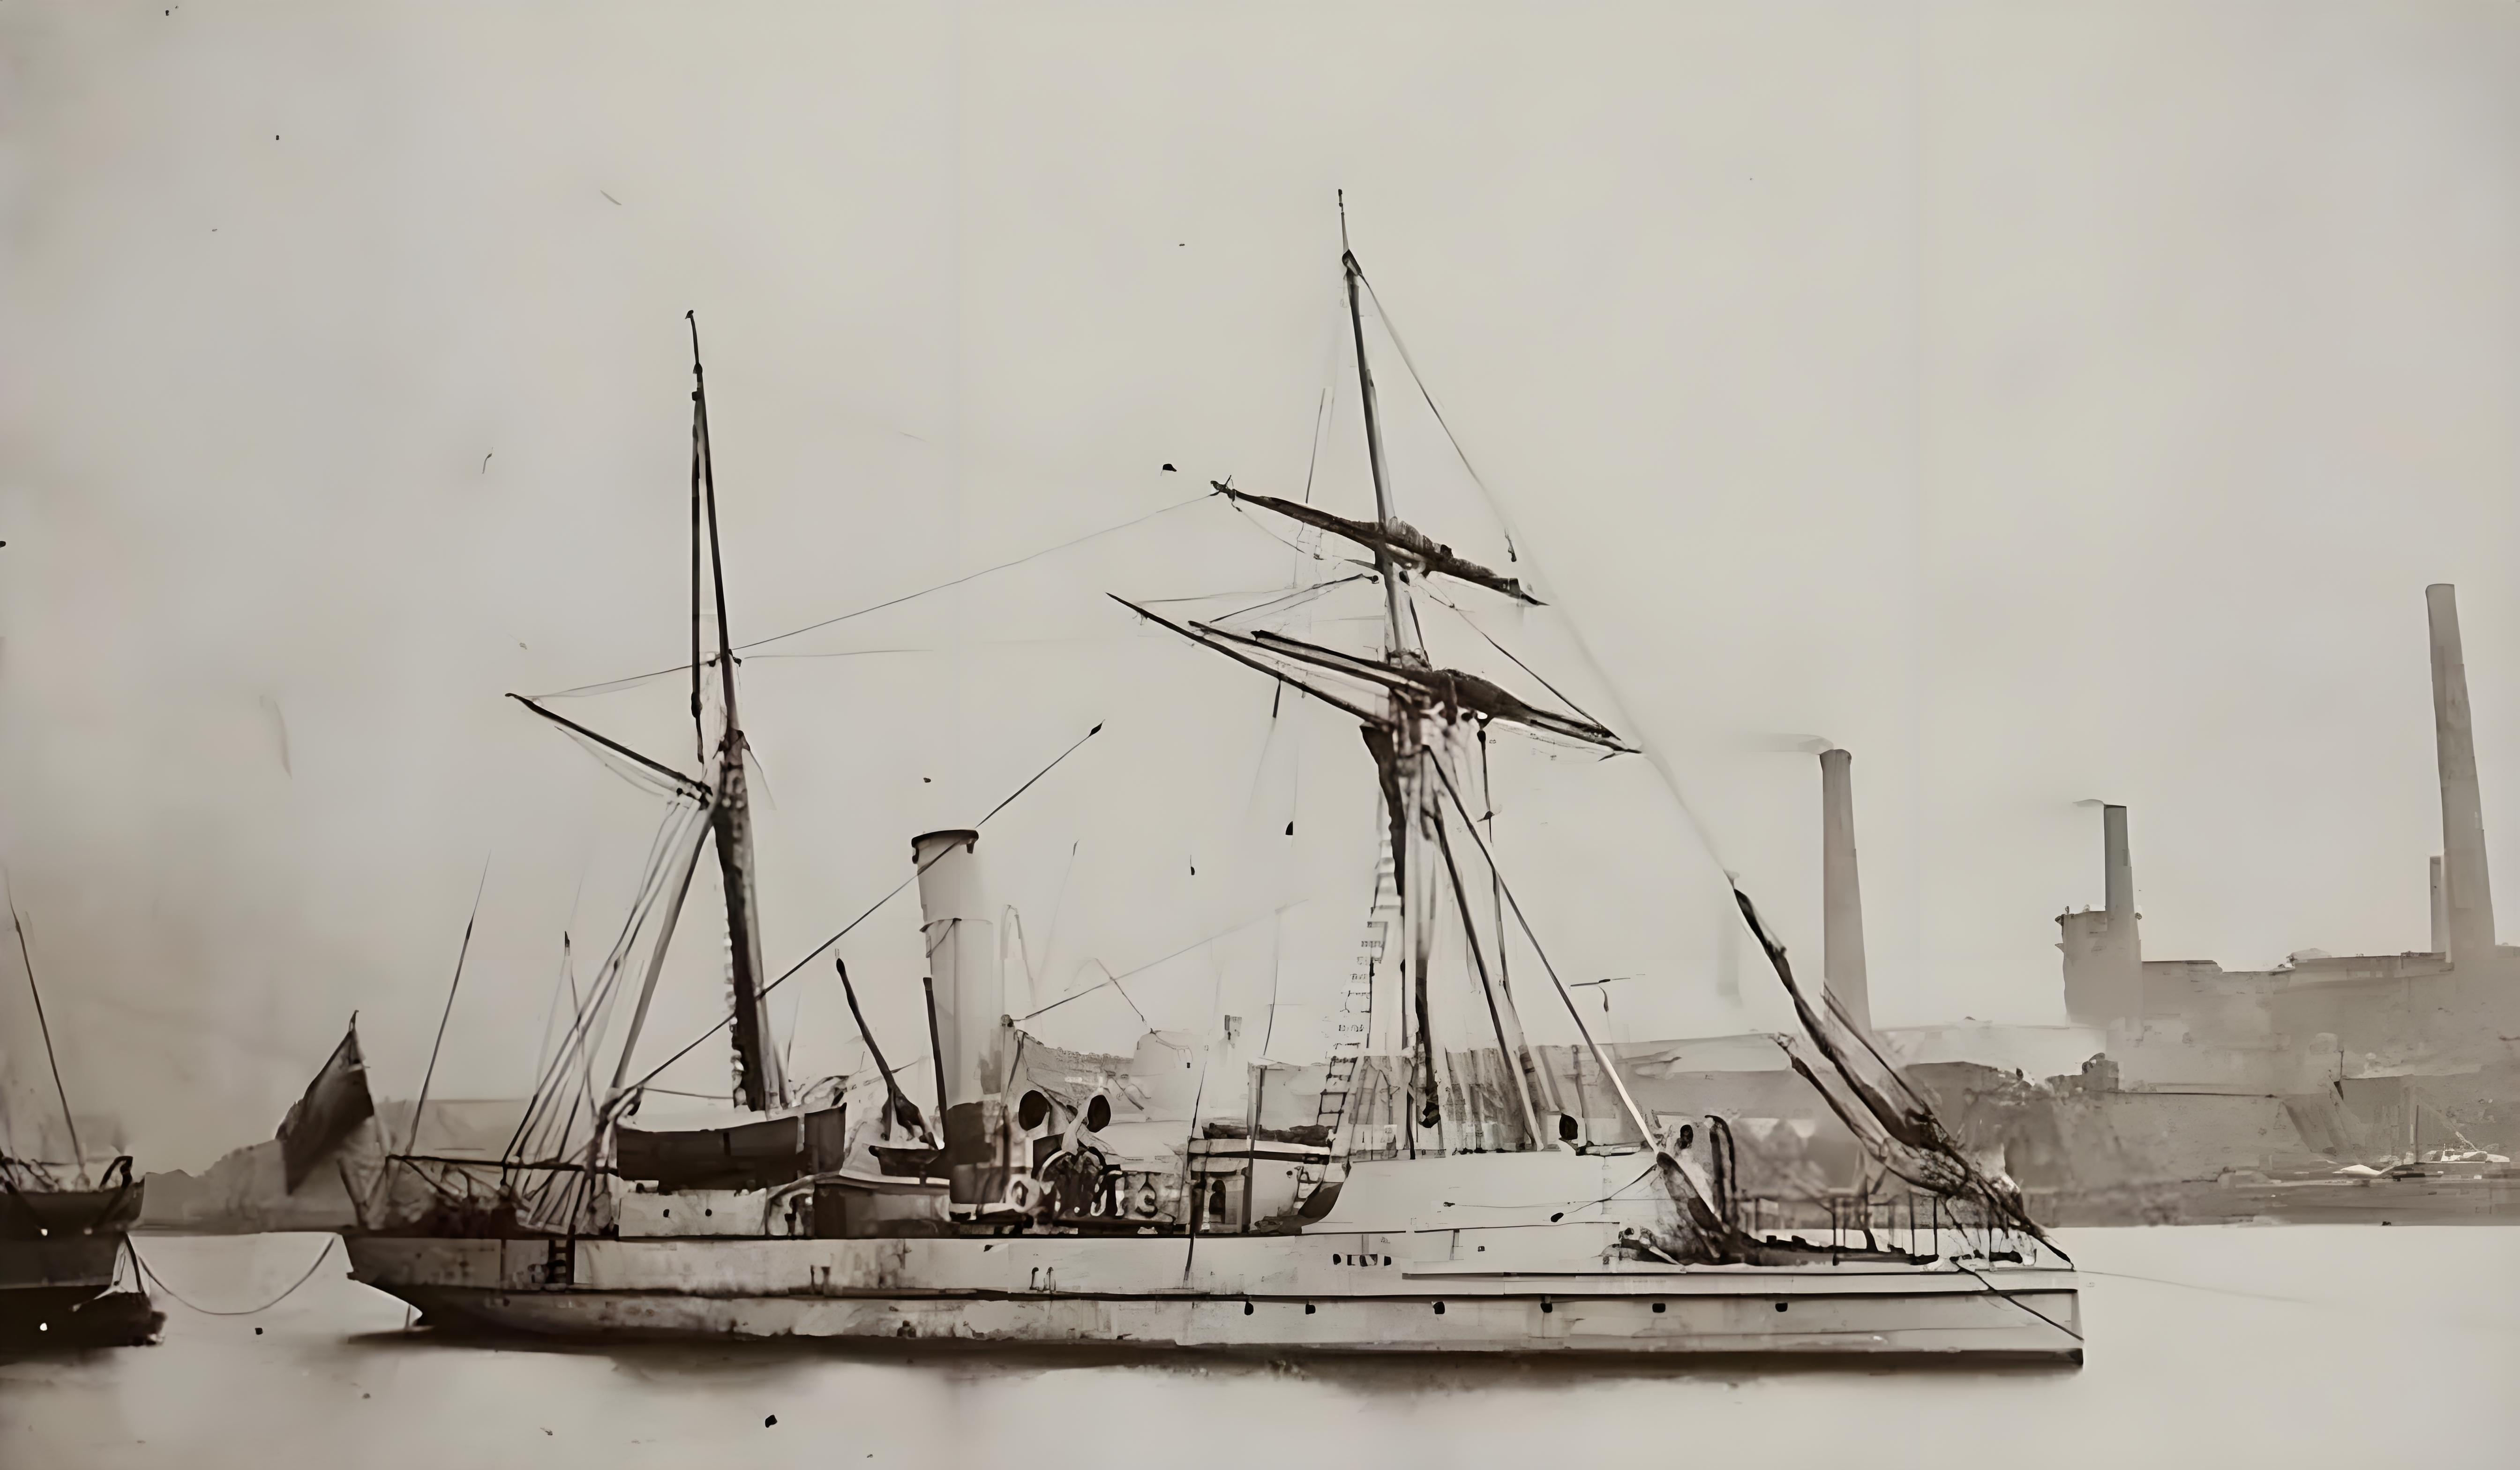
\includegraphics[width=1\linewidth]{Images/7}
	\caption{整装待发、准备回国的“戴而塔”舰,舰首舷侧的Delta舰名清晰可见,舰艉飘扬的则是英国商船旗。由于蚊子船自身煤舱容量很小,难以作远距离航行,中国的蚊子船都添加了桅杆的设计,以便必要时借助风力航行。}
	\label{fig:1}
\end{figure}

综合来看,2级新型军舰长宽比都较小,体形短粗,而且主机功率小,航速迟缓,并不适宜远航,的确只是守护海岸的水炮台而已。似乎是为了要做更进一步的诠释,“伽马”级在舰艏弹药库装满标配的50发炮弹后,如果不在舰艉加装10吨或12吨压舱物,则舰艏将要淹没在水面之下,这样的船,显然不是用于海战的。

4艘新军舰的建造过程非常顺利,“阿尔法”“贝塔”分别于1876年2月23日和4月13日顺利下水,\footnote{Peter Brook:Warships for Export-Armstrong War是平时1867-1927,1999,p30.}6月5日,金登干和英国海军部首席舰船设计师查看了2舰,表示非常满意。\footnote{《金致赫第94号》,《中国海关密档》8,北京:中华书局1995年版,第78页。}6月14日,米切尔船厂里一片热闹,意大利、丹麦等对蚊子船抱有浓厚兴趣的国家,纷纷派出武官来现场参观为中国建造的这2艘最新式蚊子船的试航,“阿尔法”“贝塔”按照英国海军部的规定,主炮用实弹和教练弹试射4次,军舰试航后航速达到9节,符合合同要求,英国海军部立刻出具证书,2艘军舰试航成功。\footnote{《金致赫第95号》,《中国海关密档》8,北京:中华书局1995年版,第78-79页。}

遵照李鸿章“每船制成两只,随时先送来中国天津口查验,不必俟全行制就一并送来”的要求,\footnote{《与赫总税司议定购办船炮章程》,《李鸿章全集》31,合肥:安徽教育出版社2008年版,第198页。}6月24日,在英国船长勒莫提·拉普利曼达吉,以及汉密尔顿指挥下,“阿尔法”、“贝塔”由雇佣的英国水手驾驶,踏上返回中国的航程。考虑到2艘仅有320吨的小船要涉渡重洋,每舰分别投了30000英镑的高额保险。\footnote{《金致赫第95号》,《中国海关密档》8,北京:中华书局1995年版,第78-80页。}

此后经过漫长的航行,虽然中途遇到风暴袭击,但一切有惊无险,于11月20日抵达天津塘沽。因为蚊子船上空间狭小,除了舰长室外,根本没有考虑水兵的居住空间,整个航程中,护送的英国水手必须在甲板上搭设帐篷露宿,艰劳程度可以想像。27日,李鸿章与赫德兴致勃勃亲往验收,李鸿章对军舰表示满意,认为“实系近时新式,堪为海口战守利器”,给予了2个极为威武的名字“龙骧”、“虎威”(Lung Hsiang,Hu Wei),并商调船政后学堂毕业生张成、邱宝仁分别管带。\footnote{《光绪二年十月二十日直隶总督李鸿章奏折附片》,中国近代史资料丛刊《洋务运动》2,上海:上海人民出版社1961年版,第345-346页。}赫德对这次的检阅情况却始终心有余悸,因为检阅过程中,出现了意外的事故,一名英国水手晕头晕脑,手中的步枪竟然走火,子弹紧贴着李鸿章的头顶飞过,当时李鸿章幸亏是坐着的,否则后果不堪设想,中国的近代史差点就将改写,这一火暴的插曲使赫德对此后的送舰活动充满了顾虑。\footnote{《中国海关密档》1,北京:中华书局1995年版,第534页。}接收之后,时值寒冬,李鸿章担心北方缺乏合适船坞设施,命令张成、邱宝仁率舰前往船政选募船员,又因为当时中日在琉球等问题上关系日益紧张,应福建巡抚丁日昌有关加强台澎防护的请求,“龙骧”、“虎威”由张成统领布置到台湾巡防。帮助驾驶2舰来华的英国船员,除每舰暂留3名技术军官充当教习外,其余均迅速遣返回国。

\begin{figure}[htbp]
	\centering
	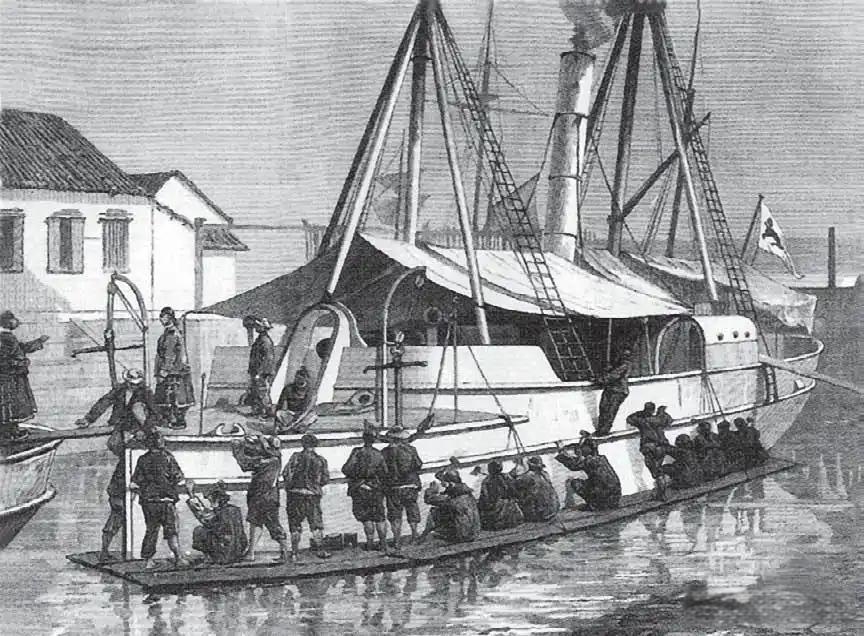
\includegraphics[width=1\linewidth]{Images/8}
	\caption{西方报纸刊登的铜版画,表现的是“阿尔法”回国后,中国工程技术人员对其进行检修、维护的情形。}
	\label{fig:1}
\end{figure}

“龙骧”、“虎威”2艘新式蚊子船整装开往遥远东方的祖国时,“伽马”、“戴而塔”在1876年6月14、23日先后下水,1877年2月17日在英国朴茨茅斯进行航试(此前在纽卡斯尔已经测得“伽马”的平均航速超过9.5节,“戴而塔”的平均航速为9节,符合设计要求。)英国海军界重要将领,以及各国驻英要员出席了试航仪式,中国驻英公使郭嵩焘亲临现场,并亲手演放了“伽马”舰的12.5英寸口径巨炮。到场参观的英国海军上将斯图尔特(Stewart),对中国的蚊子船给予高度评价:“一个真正的水兵只要一踏上船就会感到,这正是他所要的东西,是应用机械科学最渊博的知识来满足水兵的最真实的利益和需要的东西。”\footnote{《中国海关密档》1,北京:中华书局1995年版,第509页。}

第一次体验炮手工作的郭嵩焘显得非常兴奋,在当天的日记中饶有兴味地记下了蚊子船火炮系统的结构以及试炮的经过:

“初五日,金登干约至波斯莫斯观所造铁甲小船(蚊子船),安炮船首,外设炮墙护之,内复施墙,置机器。进退高低各设一机器,外推则进,内推则退,高低亦然。先推使退向内,低承前罶下(指先将炮口俯下装填弹药);而后转火药炮子以当炮口。前罶下复设机器,内推则机器直送入炮口,带水洗膛。次第送火药及炮子入,乃推置前罶下;乃复起炮使高,以度测之,而后推出炮墙外。又设电气线于机器墙内,引手按之,而声发子出,可及七千五百余步。但得一人,运机器有余,可云神妙……其‘代拉塔’(戴而塔)船亦开出海口,各演炮三,内演试群子一,船旁小炮及连环子炮皆历试之,亦平生之创见矣……”\footnote{郭嵩焘:《伦敦与巴黎日记》,长沙:岳麓书社1984年版,第117页。}

赫德担心送舰交货时再出现类似枪支走火的事故,反复叮嘱金登干加以注意,金登干起初想转嫁责任,准备干脆让阿姆斯特朗公司派人送船,最后则设法与皇家海军磋商,在确认运送的船只是最先进的军舰后,皇家海军破例批准可以让现役军官以请假的形式接受雇佣。两名现役军官琅威理(William M Lang)、劳伦斯·庆随后就被雇佣来管理驾驶“伽马”、“戴而塔”送往中国。

有现役英国军官驾驶运送,按理因当万无一失,金登干于是向赫德打包票:“您看吧!这些炮艇移交时准能像英国战舰那样——秩序井然,水手严守岗位。我认为,如果李鸿章不看一看炮艇上的英国水手是怎样操纵大炮的,那真是太可惜了……精心选拔的船员,将可充分利用这次出航的机会,来熟习和发挥这些舰只的性能。我毫不怀疑“伽马”和“戴而塔”号炮艇将以最漂亮的军舰的姿态驶抵中国。因此到达那里以后,要使各个有关方面都感到满意,这些炮艇应该受到李鸿章本人的正式视察,以使他了解到,在称职的人手操作下,这些炮艇可以达到多么高的效能。”\footnote{《中国海关密档》1,北京:中华书局1995年版,第503页。}

2月28日傍晚6点半,盘旋在英伦的恶劣天气稍稍平息,皓月当空,“伽马”、“戴而塔”鱼贯驶入英吉利海峡,踏上回国的航程。有趣的是,当时的中国公文将送舰的两位英国军官的名字分别音译为浪为美、静乐林,取风平浪静的吉祥之意,\footnote{《复福建船政吴春帆京卿》,《李鸿章全集》32,合肥:安徽教育出版社2008年版,第22页。}其中浪为美——琅威理尤其受到郭嵩焘的好评。站在飞桥上指挥若定的琅威理,脑海里可能还在想着热恋中的女友,但从这次航程开始,这个英国人与中国的海军建设结下了深深的缘分。

尽管从“伽马”、“戴而塔”出发开始,金登干就不厌其烦地向赫德介绍护送蚊子船的英国海军军官之可靠,介绍每个人的才干,甚至还把琅威理电报发回的航行日志转发给赫德。然而赫德仍然感觉不放心,要求2艘蚊子船不用直驶大沽,先前往福建船政,等自己查看后再作决断。

6月18日,“伽马”、“戴而塔”顺利到达了位于福州马尾的船政,赫德发现“它们在到达时,还不如‘阿尔法’、‘贝塔’号驶抵天津时干净、整洁”,于是决定就在福州就地交付给中国,以免去天津旁生枝节。“经过同船员们谈话,并注意看了水手们的外貌,我决定不让他们去天津,它们决不会给李留下什么特殊的印象。”\footnote{《中国海关密档》1,北京:中华书局1995年版,第561页。}6月25日,2艘蚊子船直接在船政移交中国,随即被李鸿章分别命名为“飞霆”、“策电”(Fei Ting、Tse Tien),连同先到的“龙骧”、“虎威”被重新分派军官,由从船政借调的军官邓世昌、李和、邱宝仁、吴梦良分别管带,就近在福州一带募集船员。\footnote{《复吴春帆京卿》,《李鸿章全集》32,合肥:安徽教育出版社2008年版,第40页。}

\section{蚊子船热}

“龙骧”等4艘新式军舰成功回国,立刻在中国国内引起轰动,对这种据说能够打败铁甲舰的海防利器,沿海各省纷纷表示羡慕。实际在作为国家行为的北洋购买蚊子船之前,中国沿海很多地方早已经有了购造蚊子船的活动。1875年,福建善后局就曾通过上海载生洋行向英国莱尔德公司(Cammell Laird)订购了2艘蚊子船,分别命名“福胜”、“建胜”(Fu Sheng、Chen Sheng),首开中国购买蚊子船的先河。这两艘后来移交福建船政的蚊子船,排水量256吨,长26.52米,宽7.92米,吃水2.51米,小于“阿尔法”级,主机功率180匹马力,航速8节,装备1门10英寸口径瓦瓦苏尔(Vavasseur)前膛火炮。\footnote{Richard N J Wright,The Chinese Steam Navy 1862--1945,Chatham Publishing 2000,p42;Conway's All The World's Fighting Ships 1860--1905,Conway Maritime Press 1979,p398.}而看到北洋新购的“龙骧”、“虎威”等新式蚊子船,福建巡抚丁日昌认为性能胜过“福胜”、“建胜”,主张立刻按照北洋购买的样式,为福建海防增购一批。

\begin{figure}[htbp]
	\centering
	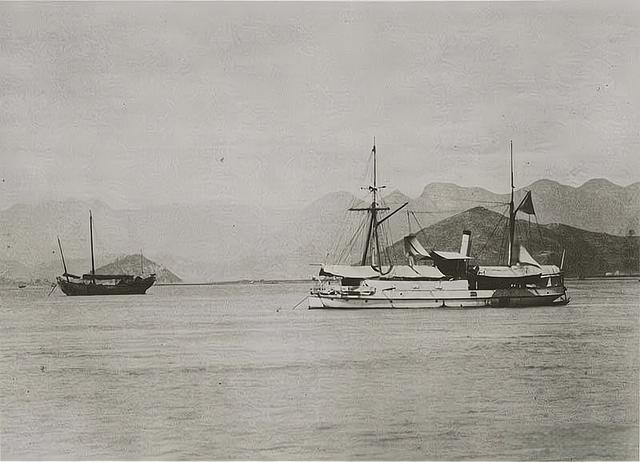
\includegraphics[width=1\linewidth]{Images/9}
	\caption{1884年中法马江之战前,停泊在马江江面的“福胜”级蚊子船。}
	\label{fig:1}
\end{figure}

与福建几乎同时,南洋治下的江南机器制造总局于1875年9月15日下水了一艘自造的蚊子船。这艘名为“金瓯”(TiongSing),寓意江山永固的军舰,诞生得极为突兀,可以看作是当时中国的军工技术人员紧密关注世界舰船发展潮流的结果。军舰排水量较小,仅有195吨(另有排水量200吨的记载),舰长31.7米,宽6.2米,吃水2.06米,主机功率304匹马力,航速10节,装备170毫米口径克虏伯后膛大炮1门。\footnote{Richard N J Wright,The Chinese Steam Navy 1862--1945,Chatham Publishing 2000,p36;Conway's All The World's Fighting Ships 1860--1905,Conway Maritime Press 1979,p398.}粗眼看来,这艘军舰除了采用后膛火炮,在当时各种蚊子船中略显时髦外,其他各项指标并不突出,似乎是泛泛之作。然而,“金瓯”实际是世界上第一艘装甲蚊子船(或称近海防御铁甲舰),中国的工厂技术人员们在这艘蚊子船上,率先引用了水线带装甲的设计,军舰沿水线装有厚2又3/4英寸的装甲,这一创举,比欧洲第一艘装甲蚊子船德国的Wespe要早。军舰主甲板上设置了一个带有2又3/8英寸厚装甲的炮塔,炮塔内还参照了西方地井炮的设计思路,通过液压装置,装填时将火炮降到舱内,装填完毕后则举升到炮台内,极为灵便。此外,“金瓯”舰在船艏还安装有撞角,“船头有铁杆一支,直伸出船外,如犀之独角”,\footnote{《申报》,1875年1月1日。}这又是蚊子船发展史上的一项创举。这艘外形不起眼,但实际运用了大大领先世界设计思想的军舰,简直可以视作是新技术的试验平台,诞生伊始就引起了西方世界的震惊,认为“灿烂可观”,而且很有可能的是,德国Wespe军舰设计之初的灵感,就来自于中国的“金瓯”,如果这一点能得到确认,那么“金瓯”将是包括“经远”在内的德系装甲巡洋舰的共同始祖。但是,这艘造价仅为62586.93两白银的军舰可能因为体量太小,并未引起中国国内过多的关注,当北洋的蚊子船回国后,南洋大臣沈葆桢即写信给李鸿章,请求能分拨1、2艘西方建造的蚊子船。

最后,甚至连英国人都来凑热闹了。1878年5月24日中午,天津英国领事馆内空气异常凝重,应英国人之邀前来赴宴的李鸿章,发现领事馆餐厅里仅有领事和3名英国海军军官而已。受克里米亚战争影响,英国担心俄罗斯借地利之便,到中国海域来攻击英国船只,为了加强在远东的海军力量,与李鸿章商谈,希望能将“龙骧”、“飞霆”级军舰全部购回,加入皇家海军防守香港、新加坡。考虑到中国海防建设刚刚起步,而且这4艘蚊子船自用尚且不够,李鸿章予以一口回绝。由此也可以看出,蚊子船这种船型,在当时各国海军中,仍属于利器一类。英国领事曾坦率地说“此式炮船……专防本国海口以作水炮台抵御铁甲,最为得力。”\footnote{《论英使密购回蚊船》,《李鸿章全集》32,合肥:安徽教育出版社2008年版,第304页。}

由4艘新型蚊子船回国,一时间,从南到北,中国沿海兴起了一股沸沸扬扬的蚊子船热。

鉴于各省纷纷要求购买蚊子船的情况,总理衙门致信李鸿章,称“此项船只,无论各海口,难资分布,即咽喉要区,根本重地尚不足数,必应即时添置”,要求李鸿章负责具体经办,尽快再增加购买一批蚊子船。当时,赫德已经返回阔别12年的家乡英国休假,顺道帮助具体操办中国参加巴黎世博会一事,李鸿章于是通过赫德在中国的内弟,海关总理文案税务司裴式楷(Mattbew Boyd Bredon)致电金登干,打听蚊子船的报价是否有变化。1878年7月8日上午,金登干收到了裴式楷由上海发来的电报:“目前情况下,‘阿尔法’或‘伽马’级炮艇实价几何,25163(暗号,可能代指李鸿章)询问,或许将订购四艘。”\footnote{《中国海关密档》2,北京:中华书局1995年版,第44页。}

经过和阿姆斯特朗公司的谈判杀价,7月28日,赫德、金登干提交了蚊子船的报价:年内购买2艘“阿尔法”级,单价26150英镑,如果购买4艘,则便宜至25500英镑。“伽马”级购买2艘,单价33300英镑,购买4艘,单价为32500英镑。\footnote{《中国海关密档》2,北京:中华书局1995年版,第63页。}考虑到吨位和火炮口径,李鸿章未再考虑小型的“阿尔法”级,决策再购买4艘“伽马”级蚊子船,总价45万两银。1878年8月29日下午,金登干与阿姆斯特朗公司签订合同,费尽口舌后,阿姆斯特朗坚持报价不能减少一分,但可以稍做让步,答应为每艘船免费加装1门格林炮(Gatling Gun)作为赠品。\footnote{《中国海关密档》2,北京:中华书局1995年版,第100页。}

\section{“镇”字号蚊子船}

中国新订造的这批蚊子船,按照他们的4艘姐姐的传统,被金登干继续用希腊文字母暂时命名,分别为“埃普西隆”、“基塔”、“爱塔”、“西塔”(Epsilon、Zeta、Eta、Theta),工厂建造编号374、375、376、377。\footnote{Peter Brook: Warships for Export-Armstrong Warships 1867--1927,1999,p30.}由于这几艘船的设计较之最初的“伽马”级做出了大量调整、改进,因而自成“埃普西隆”级。

与母型“伽马”相比,“埃普西隆”舰体的材质改成了更坚硬的钢,外观尺寸等数据也都发生了一定变化。这级军舰排水量增加到490吨,长38.1米(全长3.7米),宽8.84米,吃水2.9米,动力系统采用2台英国霍恩索公司(R\&W Hawthorn)生产的蒸汽机,配套2台燃煤锅炉,功率472马力,双轴推进,航速10.2节,采用艏艉双舵叶。煤舱容量和“伽马”相同,正常载量50吨,最大载量60吨。\footnote{Conway's All The World's Fighting Ships 1860-1905,Conway Maritime Press 1979,p399.Peter Brook:Warships for Export-Armstrong Warships 1867-1927,1999,p31.}

军舰的武备上变动较大,“埃普西隆”放弃了“伽马”级装备的12.5英寸口径火炮,改成一门口径略小的11英寸口径阿姆斯特朗火炮。担心中国人可能一时无法理解和接受这种改变,赫德、金登干和阿姆斯特朗公司提交了详尽的备忘录进行解释,称火炮的口径虽然变小了,但由于结构的改进和发射药量的加大,火力远较老式的大口径炮猛烈有力,“中国人可能认为,炮弹越大,造成的损害也会越大。然而,炮弹所造成的损害的大小,取决于推进炮弹的火药量的多少”,\footnote{《中国海关密档》2,北京:中华书局1995年版,第122页。}而且,阿姆斯特朗提出,新式火炮的重量较老式火炮轻,省出来的重量,可以用于改进设计,进一步增加军舰的航速。对此半信半疑的李鸿章最终接受了这个改变。

\begin{figure}[htbp]
	\centering
	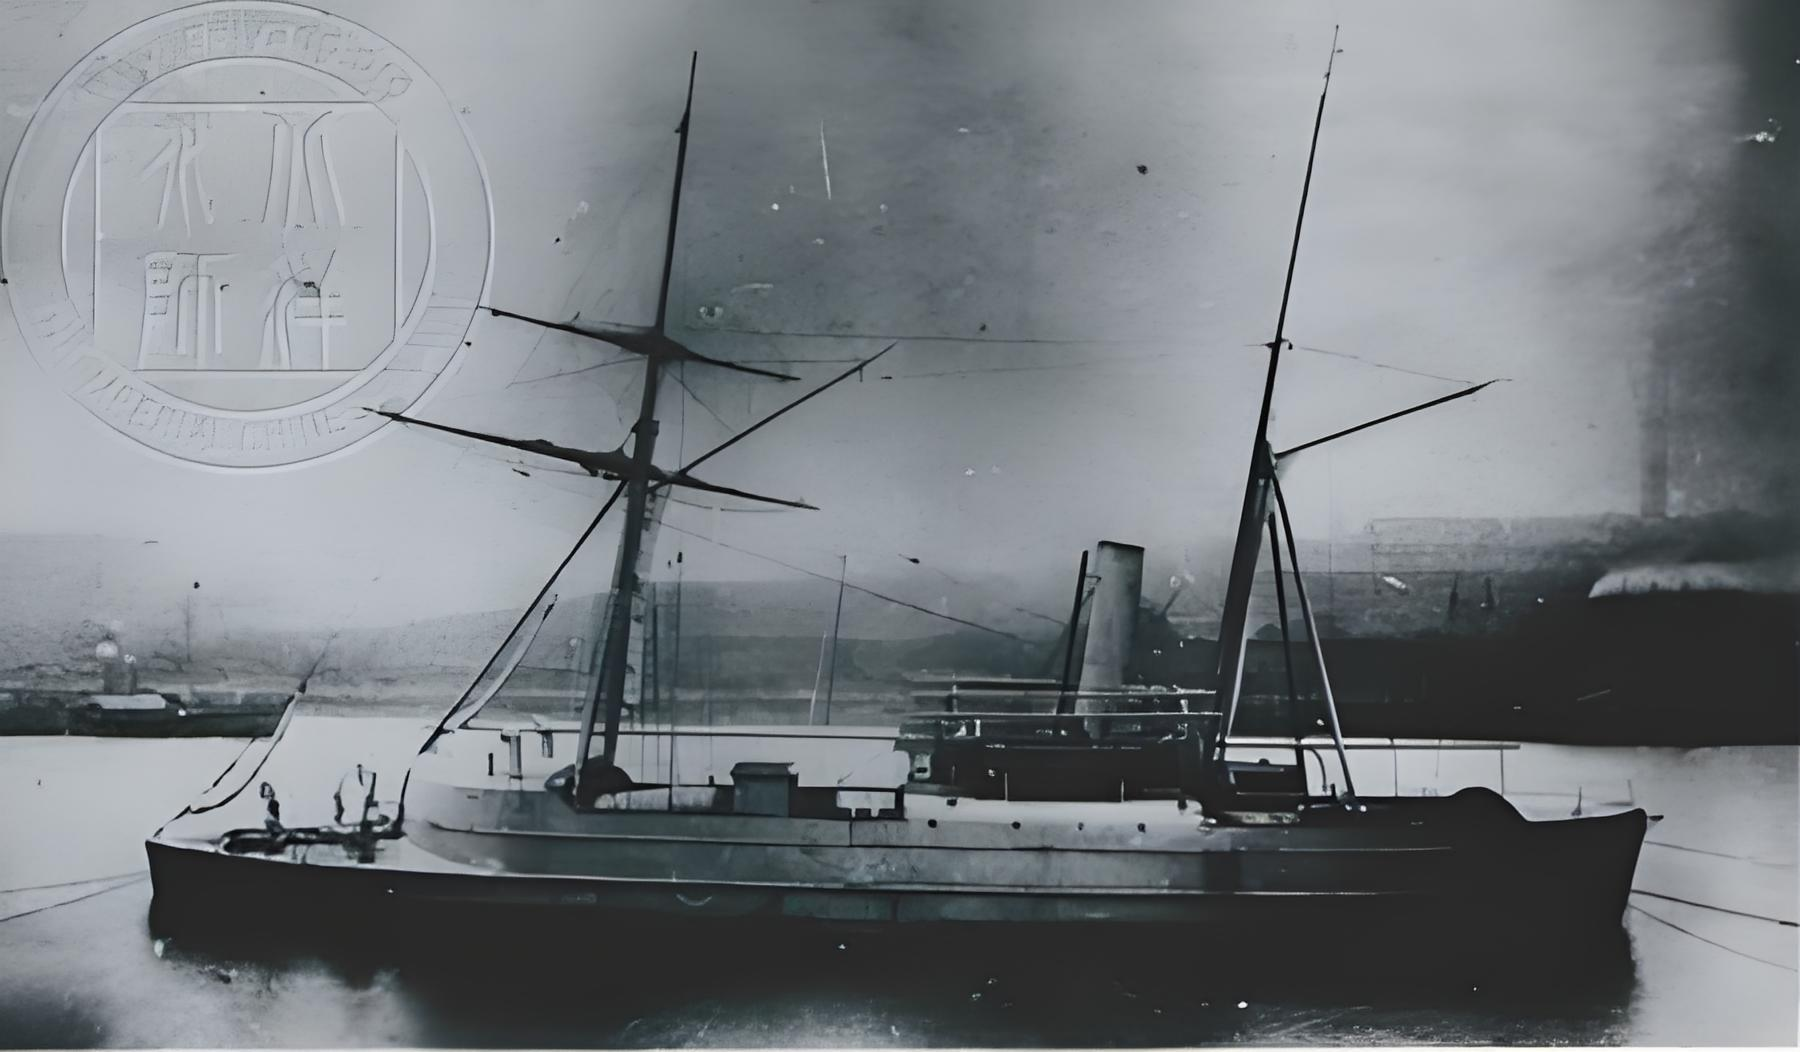
\includegraphics[width=1\linewidth]{Images/10}
	\caption{停泊在泰恩河上的“埃普西隆”“镇东”,军舰中部的飞桥上搭建了用于铺设天幕的支架。}
	\label{fig:1}
\end{figure}

新安装的11英寸口径阿姆斯特朗前装线膛火炮,实际口径279.4毫米,膛长6480毫米,弹重240.4公斤,炮重35吨,火炮初速554米/秒,射程7681米,火炮的操作以及弹药装填方式与“伽马”级相同,“大炮装在前面,用水力运转、装弹、制驭,开炮只需要5个人。瞄准时大炮的旋转并没有机械的自动设备,而是由船本身去完成回转任务……因为船身短,又装有两具推进机,所以这只小船能够依情况的需要迅速准确地旋转”\footnote{《“田凫”号航行记》,中国近代史资料丛刊《洋务运动》8, 上海: 上海人民出版社1961年版,第416页。}。此外,和“阿尔法”、“伽马”一样,主甲板上还安装有2门3英寸口径后膛炮,同样由阿姆斯特朗公司制造,实际口径76.2毫米,炮身长1920毫米,初速357米/秒,射程5800米。根据“阿尔法”、“伽马”的原先设计,军舰上还配有1门格林机关炮,因为阿姆斯特朗公司又附赠了1门,格林炮总数增加为2门。

拥有大量造舰经验的米切尔船厂,对建造这几艘小型军舰可谓驾轻就熟,建造过程一切顺利,“埃普西隆”级4艘军舰在1878年9月9日同时开工,分别于1879年1月20日、3月22日、2月5日、3月27日下水。\footnote{Peter Brook: Warships for Export-Armstrong Warships 1867--1927,1999,p30.}1879年3月25日,顾不上患病不起的妻子,金登干和曾经驾驶护送“伽马”舰前往中国的海军军官琅威理一起来到纽卡斯尔,视察了接近完工的首舰“埃普西隆”。结合在以往驾驶“伽马”远航中的切身感受,琅威理认真地对新蚊子船提出了很多修改建议,经过很长时间的辩论,伦道尔、阿姆斯特朗被说服,同意对新军舰进行某些修改。“埃普西隆”级蚊子船原本外形上和母型“伽马”非常相像,而经过这次修改后,外形上就产生了极为明显的区别。琅威理对“埃普西隆”的主要修改建议有:在主炮防护围壁上方水平敷设一块薄钢板和防波板,以便使得任何时候火炮都处于遮蔽中;将军舰的舷墙全部增高2英尺,既可以在航行时防浪,也能在战时对水手起到保护作用;将原本露天的军舰舰艉甲板,用硬质的顶棚遮护,可以免除在倒车航行时甲板上浪。\footnote{《中国海关密档》2,北京:中华书局1995年版,第182页。}经过这系列改装,“埃普西隆”的设计更加完善,成为蚊子船发展过程中的一型成熟之作。

1879年7月24日,继郭嵩焘之后出任驻英公使的曾纪泽由金登干陪同抵达朴次茅斯,一行人等分乘4艘蚊子船出海演试。在“埃普西隆”甲板下并不宽敞的餐厅内用过午饭后,曾纪泽亲手燃放舰艏的大炮,显然开炮这种带有亲身体验性质的活动很受中国官员欢迎,“炮之进退高下以及装药盛子,皆以汽机运之,启闭其机极为灵便,不过用斤许力耳。第一炮装药、盛子、进炮,皆余自启其机。”跟随在“埃普西隆”之后的“基塔”等船也各试炮2响,其中鸣响“基塔”舰大炮的是金登干的夫人,此举似乎是进一步说明蚊子船火炮系统设计之巧妙灵便。试炮完毕后,各舰又测试机动性能,360度旋回三圈,第一圈单纯靠螺旋桨,第二圈依靠舰艏舵叶,第三圈则是舰艉的舵叶,在方圆30丈的区域内,测得旋转一次平均时间为3分5秒,一切表现令人满意。\footnote{《曾纪泽集》,长沙:岳麓书社2005年版,第356页。}

7月30日,由琅威理率领,4艘“埃普西隆”级蚊子船起航回国,此前鉴于福政于1877年派出的赴欧洲海军留学生已经留学有日,为造就人才,李鸿章曾和留学生监督李凤苞协商,意图从留学生中挑选资质优良者驾驶这批蚊子船回国,不假手于西方人,然而金登干以中国学生学业未精等借口婉拒,最终仍雇用英国船员驾驶护送。

新蚊子船离开英国的当天,《泰晤士报》做出长文报道,认为这些军舰装备的火炮威力惊人,超过当时英国所有舰上火炮,表示出了对这型新式蚊子船的艳羡:“星期三清晨,在岬头(Spithead)出现了一队样式新颖的炮舰,朴次茅斯的海军界为之惊愕……它们虽然悬挂英国海军的红色旗帜,但显然不属于英国。它们是埃尔思威克工场、阿姆斯特朗公司为中国政府所建造的……中国人作此突然的冒险一跳,已经跳到我们前面去了。当人们记住这些的时候,便知道这个新创事件的重要性和所表现的勇气是值得注意了”\footnote{《“田凫”号航行记》,中国近代史资料丛刊《洋务运动》8, 上海: 上海人民出版社1961年版,第412-413页。}。

\begin{figure}[htbp]
	\centering
	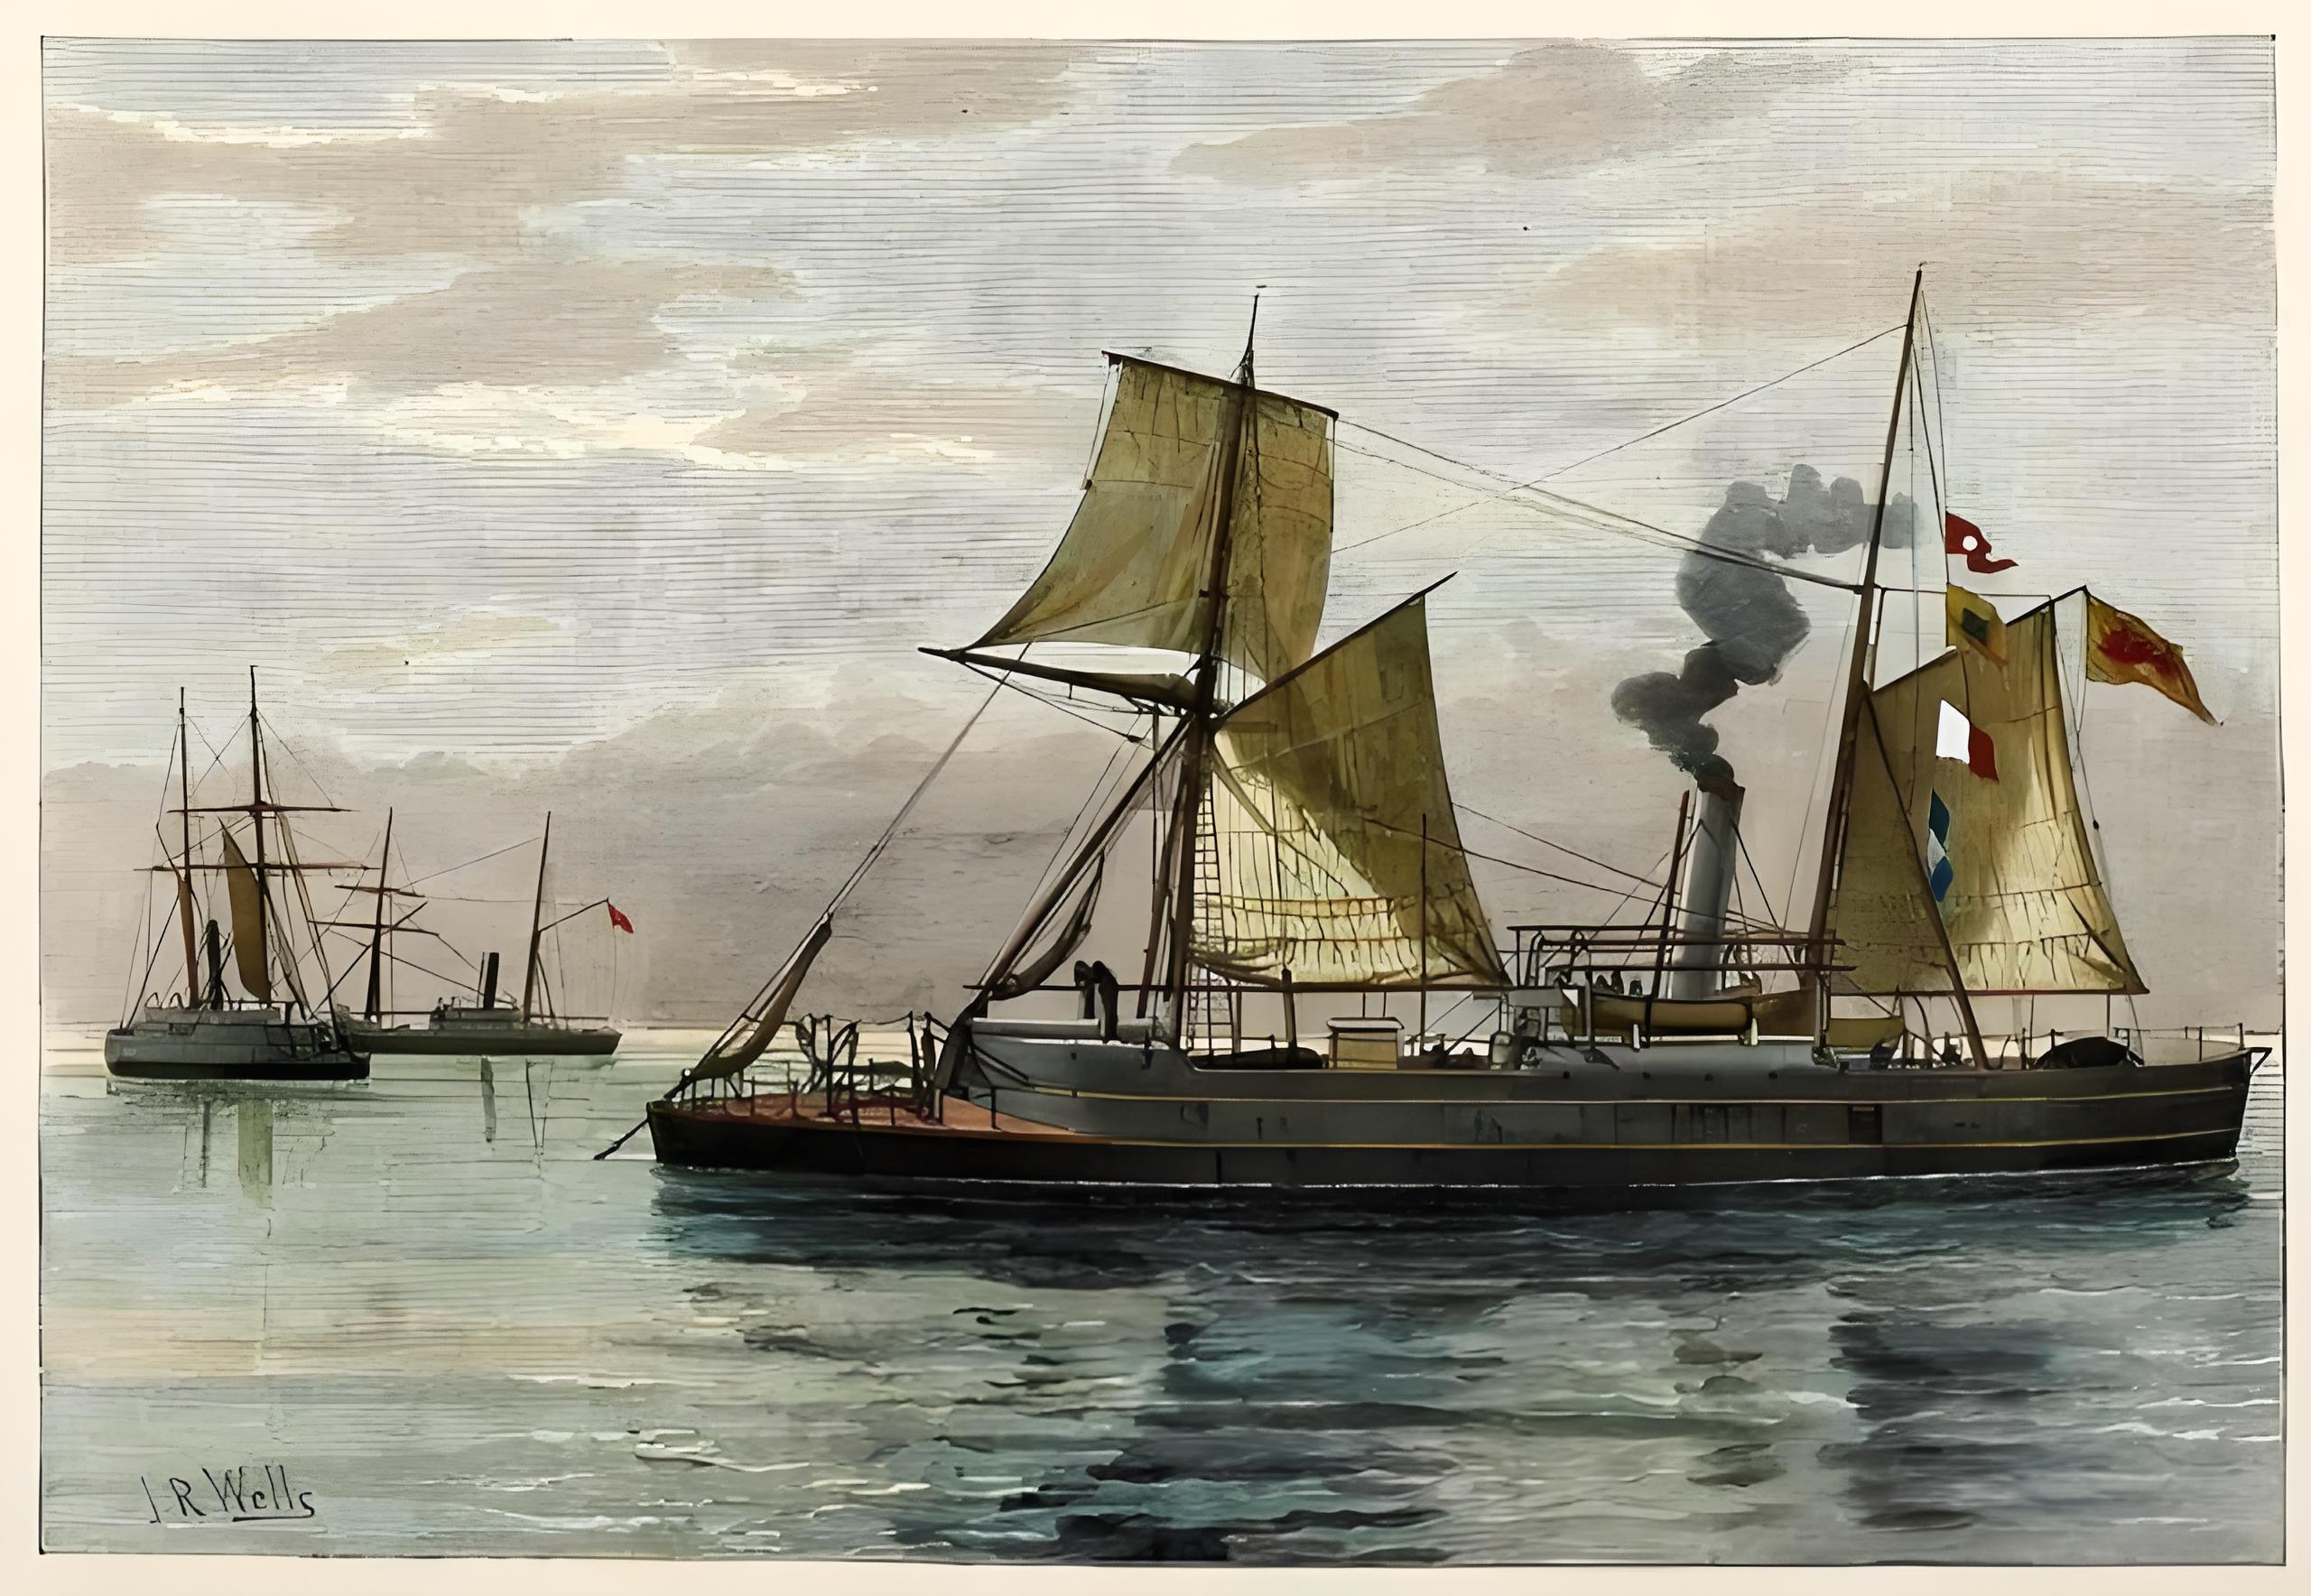
\includegraphics[width=1\linewidth]{Images/11}
	\caption{西方报纸刊载的中国蚊子船编队铜版画。蚊子船回国之初,在基本没有近代化海军基础的情况下,一度成为中国海上武装的骨干,频繁在近海出现、游弋。}
	\label{fig:1}
\end{figure}

清政府最初做出这次增购蚊子船的决策,主要是考虑到南洋大臣提出的加强南洋海防的请求,而原先购买的“龙骧”、“飞霆”等4艘军舰数量太少,不够分拨。因而,“埃普西隆”级蚊子船的订购,虽然经李鸿章之手操办,南洋大臣沈葆桢认为这些军舰将来非南洋莫属,当新式蚊子船到达中国领海后,沈葆桢亲自为四艘军舰命名为“镇北”、“镇南”、“镇西”、“镇东”(Chen Pei、Chen Nan、Chen His、Chen Tung,因而这批军舰又可以称为“镇北”级),且预备派出船政后学堂的毕业生刘步蟾等接管,就任新军舰的管带,在福州马尾等待接收新蚊子船。出乎沈葆桢预料的是,早在订立购舰合同时,李鸿章就意味深长地强调4艘新军舰必须抵达天津大沽,由他自己验收交货。为此,李鸿章还专门通过赫德,派赫德的内弟——江海关税务司赫政(James H.Hart)前往广东,抢在南洋之前迎护,一路监督新蚊子船到达天津。当年11月19日,李鸿章亲自前往大沽检阅4艘新舰,颇为满意。\footnote{中国近代史资料丛刊《洋务运动》2,上海:上海人民出版社1961年版,第418--419页。}

11月30日,李鸿章致信沈葆桢,将“龙骧”、“虎威”、“飞霆”、“策电”4艘较早购买的蚊子船调归南洋,而新购的4艘“镇”字舰留在北洋使用。\footnote{《复两江制军沈》,《李鸿章全集》32,合肥:安徽教育出版社2008年版,第493页。}书信中,李鸿章阐述了他的理由主要有2点,首先“龙骧”等蚊子船在北洋驻防已经2年,原本就需要南下上海进船坞刮修船底,将这4艘军舰调给南洋,“藉省往返”。另外,南洋预备用蚊子船驻防在长江内的吴淞、江阴,“风浪少平”,而北洋的蚊子船需要在大连湾等处航行,“镇”字蚊子船的设计改良更适合在北洋航行。对这种容易让人产生汰旧换新,占南洋便宜嫌疑的行为,李鸿章自表态度“非敢择利自卫”。沈葆桢在得到“镇”字蚊子船被调北上的消息后,也曾致信李鸿章,称“知大君子之用心突出寻常万万也。”\footnote{《沈文肃公牍》,扬州:江苏广陵古籍刻印社1997年版,第1338页。}

4艘“镇”字号蚊子船还在回国途中时,日本悍然吞并了中国属国琉球,中国海防形式极为严峻。当时的中国海防,除了自造的一批兵商两用的炮舰外,所能使用的新式军舰只有新购的蚊子船,但这些舰只都只适应近海防御,无法出远海决胜负,清政府内部有关海防的思想开始发生悄然变化,购买新式碰撞巡洋舰、大型铁甲舰的计划被提到议事日程。但于此同时,与赫德私交甚密的恭亲王奕䜣仍在申请购买一批用于防守近海的水炮台——蚊子船,援引李鸿章的奏折,奕䜣提议广东、台湾的港口防御需要各购买2艘;浙江宁波和山东烟台的港口防御需要各购买1艘,并认为“……令该督抚自行定购,似不如径由该大臣一手经理”,“将来各船购到时,并由该大臣验收”\footnote{《光绪五年十一月十三日总理各国事务衙门奕䜣等奏折附片》,中国近代史资料丛刊《洋务运动》2,上海:上海人民出版社1961年版,第427页。},浅眼看来,和南洋的4艘蚊子船一样,大有以为各省买舰为名,行增加北洋海防之实。

清政府随即同意了恭亲王增购蚊子船的奏请,指令相关各省自筹资金,认真办理,山东巡抚周恒祺很快便认购了2艘蚊子船。而两广总督刘坤一的回复则颇为勉强,环顾左右而言他,最后提出了“造舰”的主张。这年冬天,广东先斩后奏,批准完全由广东机器局总办温子绍个人捐款和设计,在广东黄埔船坞开工仿造一艘蚊子船。\footnote{《刘忠诚公遗集》,台北:台湾文海出版社1973年版,第2089--2095页。}这艘后来命名为“海东雄”(Hai Tung Hung)的军舰,设计上参考了北洋购买的“镇北”级蚊子船,排水量与其相同,为430吨,舰长也一致,同为38.1米,船宽略微增加,为9.14米,吃水2.41米,动力系统采用复合式蒸汽机,航速仅有7.5节。船头装备1门11英寸口径后膛炮,另外配备2门2.75英寸后膛副炮,全舰造价仅为3.39万两银。按照温子绍的设计,“海东雄”不采用英制蚊子船木壳船体外包裹铁皮的做法,直接采用纯木壳,只在部分重要部位敷设铁皮装甲,这样可以避免锈蚀,又可以节省工料节约经费,而且减轻船的吨重,使航行更为便捷。另外,“海东雄”舰艏的火炮改为后膛炮,不光装填方便,而且重量比前膛炮大大减轻,增加了船的稳性,也降低了发射时的后坐力。刘坤一以此为例,申请国家拨款再自造一艘同样的蚊子船,以替代购舰的方案。\footnote{Conway's All The World's Fighting Ships 1860-1905,Conway Maritime Press 1979,p399.}孰料这个建议被驳回,两广最后被迫也认购1艘蚊子船。

\begin{figure}[htbp]
	\centering
	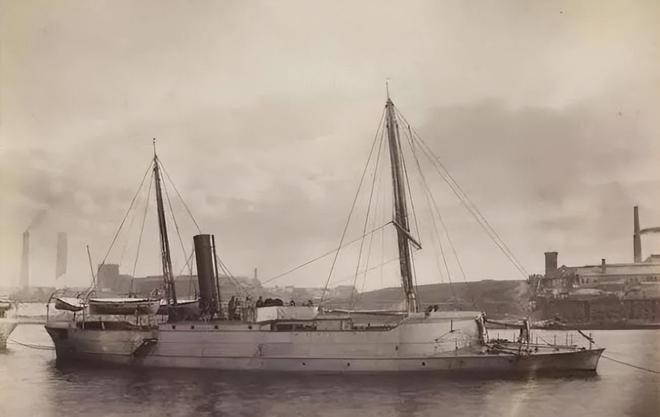
\includegraphics[width=1\linewidth]{Images/12}
	\caption{停泊在纽卡斯尔港边的“约塔”“镇边”舰,可以注意这级舰区别于“埃普西隆”的重要特征——前桅杆上只有一根横桁。}
	\label{fig:1}
\end{figure}

\begin{figure}[htbp]
	\centering
	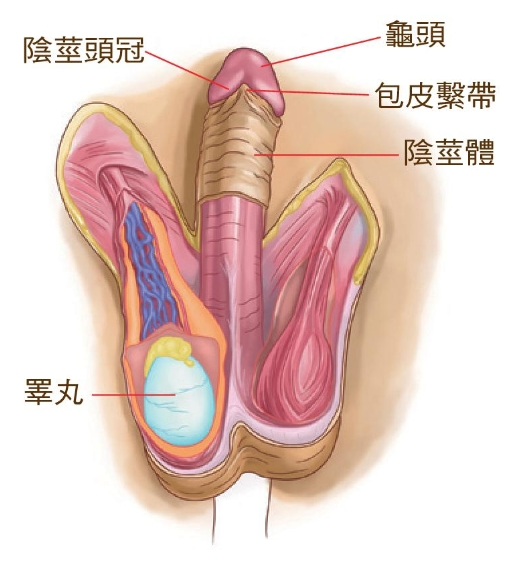
\includegraphics[width=1\linewidth]{Images/13}
	\caption{在英国船坞里进行舾装的中国蚊子船,可能是“镇中”或“镇边”。照片中能清楚看到船艏水线下的舵叶、主炮围壁上的龙纹,以及从“埃普西隆”级开始,依据琅威理的建议在主炮围壁顶上加装的防浪板。}
	\label{fig:1}
\end{figure}

仍然由赫德经手,中国向阿姆斯特朗公司又订购了3艘蚊子船,临时用希腊文字母命名为“约塔”“卡帕”“兰姆达”(Iota、Kappa、Lambda),船体仍然由劳沃克船厂建造,工厂编号411、412、413,于1880年6月2日同时开工,同年12月9日、31日、22日分别下水,1881年4月通过航试。\footnote{Peter Brook:Warships for Export-Armstrong Warships 1867-1927,1999,p31.}由山东付款的前2艘后来被分别命名为“镇中”、“镇边”(Chen Chung、Chen Pien);两广心不甘情不愿认购的那艘,后来被命名为“海镜清”(Hai Ting Ching)。

3艘船为同级,外形各项参数和此前北洋购买的“镇北”级基本相同,外形上主要的区别是,这级军舰前桅杆只有一根横桁,不同于之前中国外购的其他蚊子船。这型蚊子船排水量500吨,长38.1米,宽8.84米,吃水2.9米,动力系统采用2台霍索恩公司造蒸汽机、2台燃煤锅炉,双轴推进,功率455马力,航速10.4节,武备则和“镇北”级完全一样。\footnote{Conway's All The World's Fighting Ships 1860-1905,Conway Maritime Press 1979,p399.}

1881年夏,3舰建造完毕由英国水手驾驶回中国,7月25日到达广州时,“海镜清”被两广留用,而剩下原本由山东订购的“镇边”、“镇中”则在8月11日抵达大沽后,不出所料,被借调北洋水师使用。由此,中国的海防队伍中,共出现了15艘蚊子船。

\begin{figure}[htbp]
	\centering
	
\includegraphics[width=1\linewidth]{Images/14}
	\caption{“约塔”级蚊子船艉部照片,可以看到装饰于船艉的龙纹以及船底侧面的舭龙骨。}
	\label{fig:1}
\end{figure}

\begin{figure}[htbp]
	\centering
	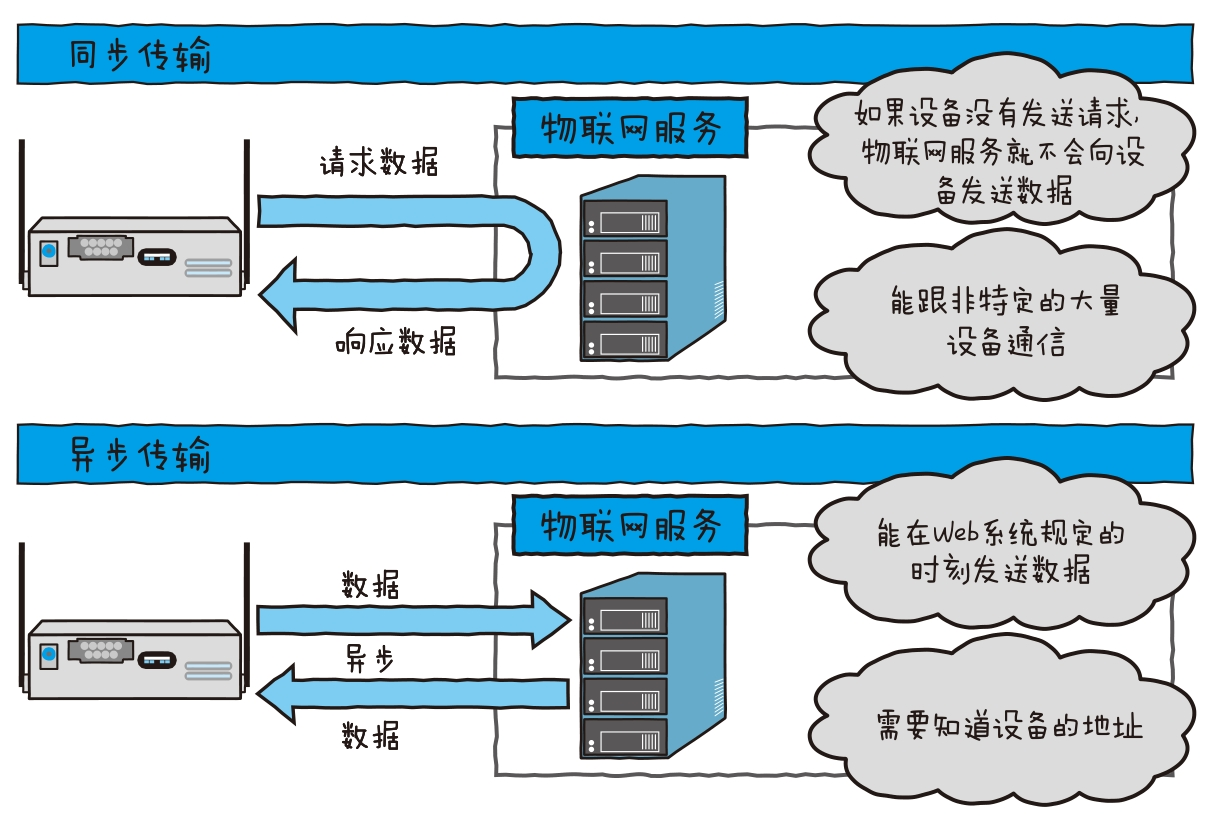
\includegraphics[width=1\linewidth]{Images/15}
	\caption{“约塔”级蚊子船的主炮位。}
	\label{fig:1}
\end{figure}

\begin{figure}[htbp]
	\centering
	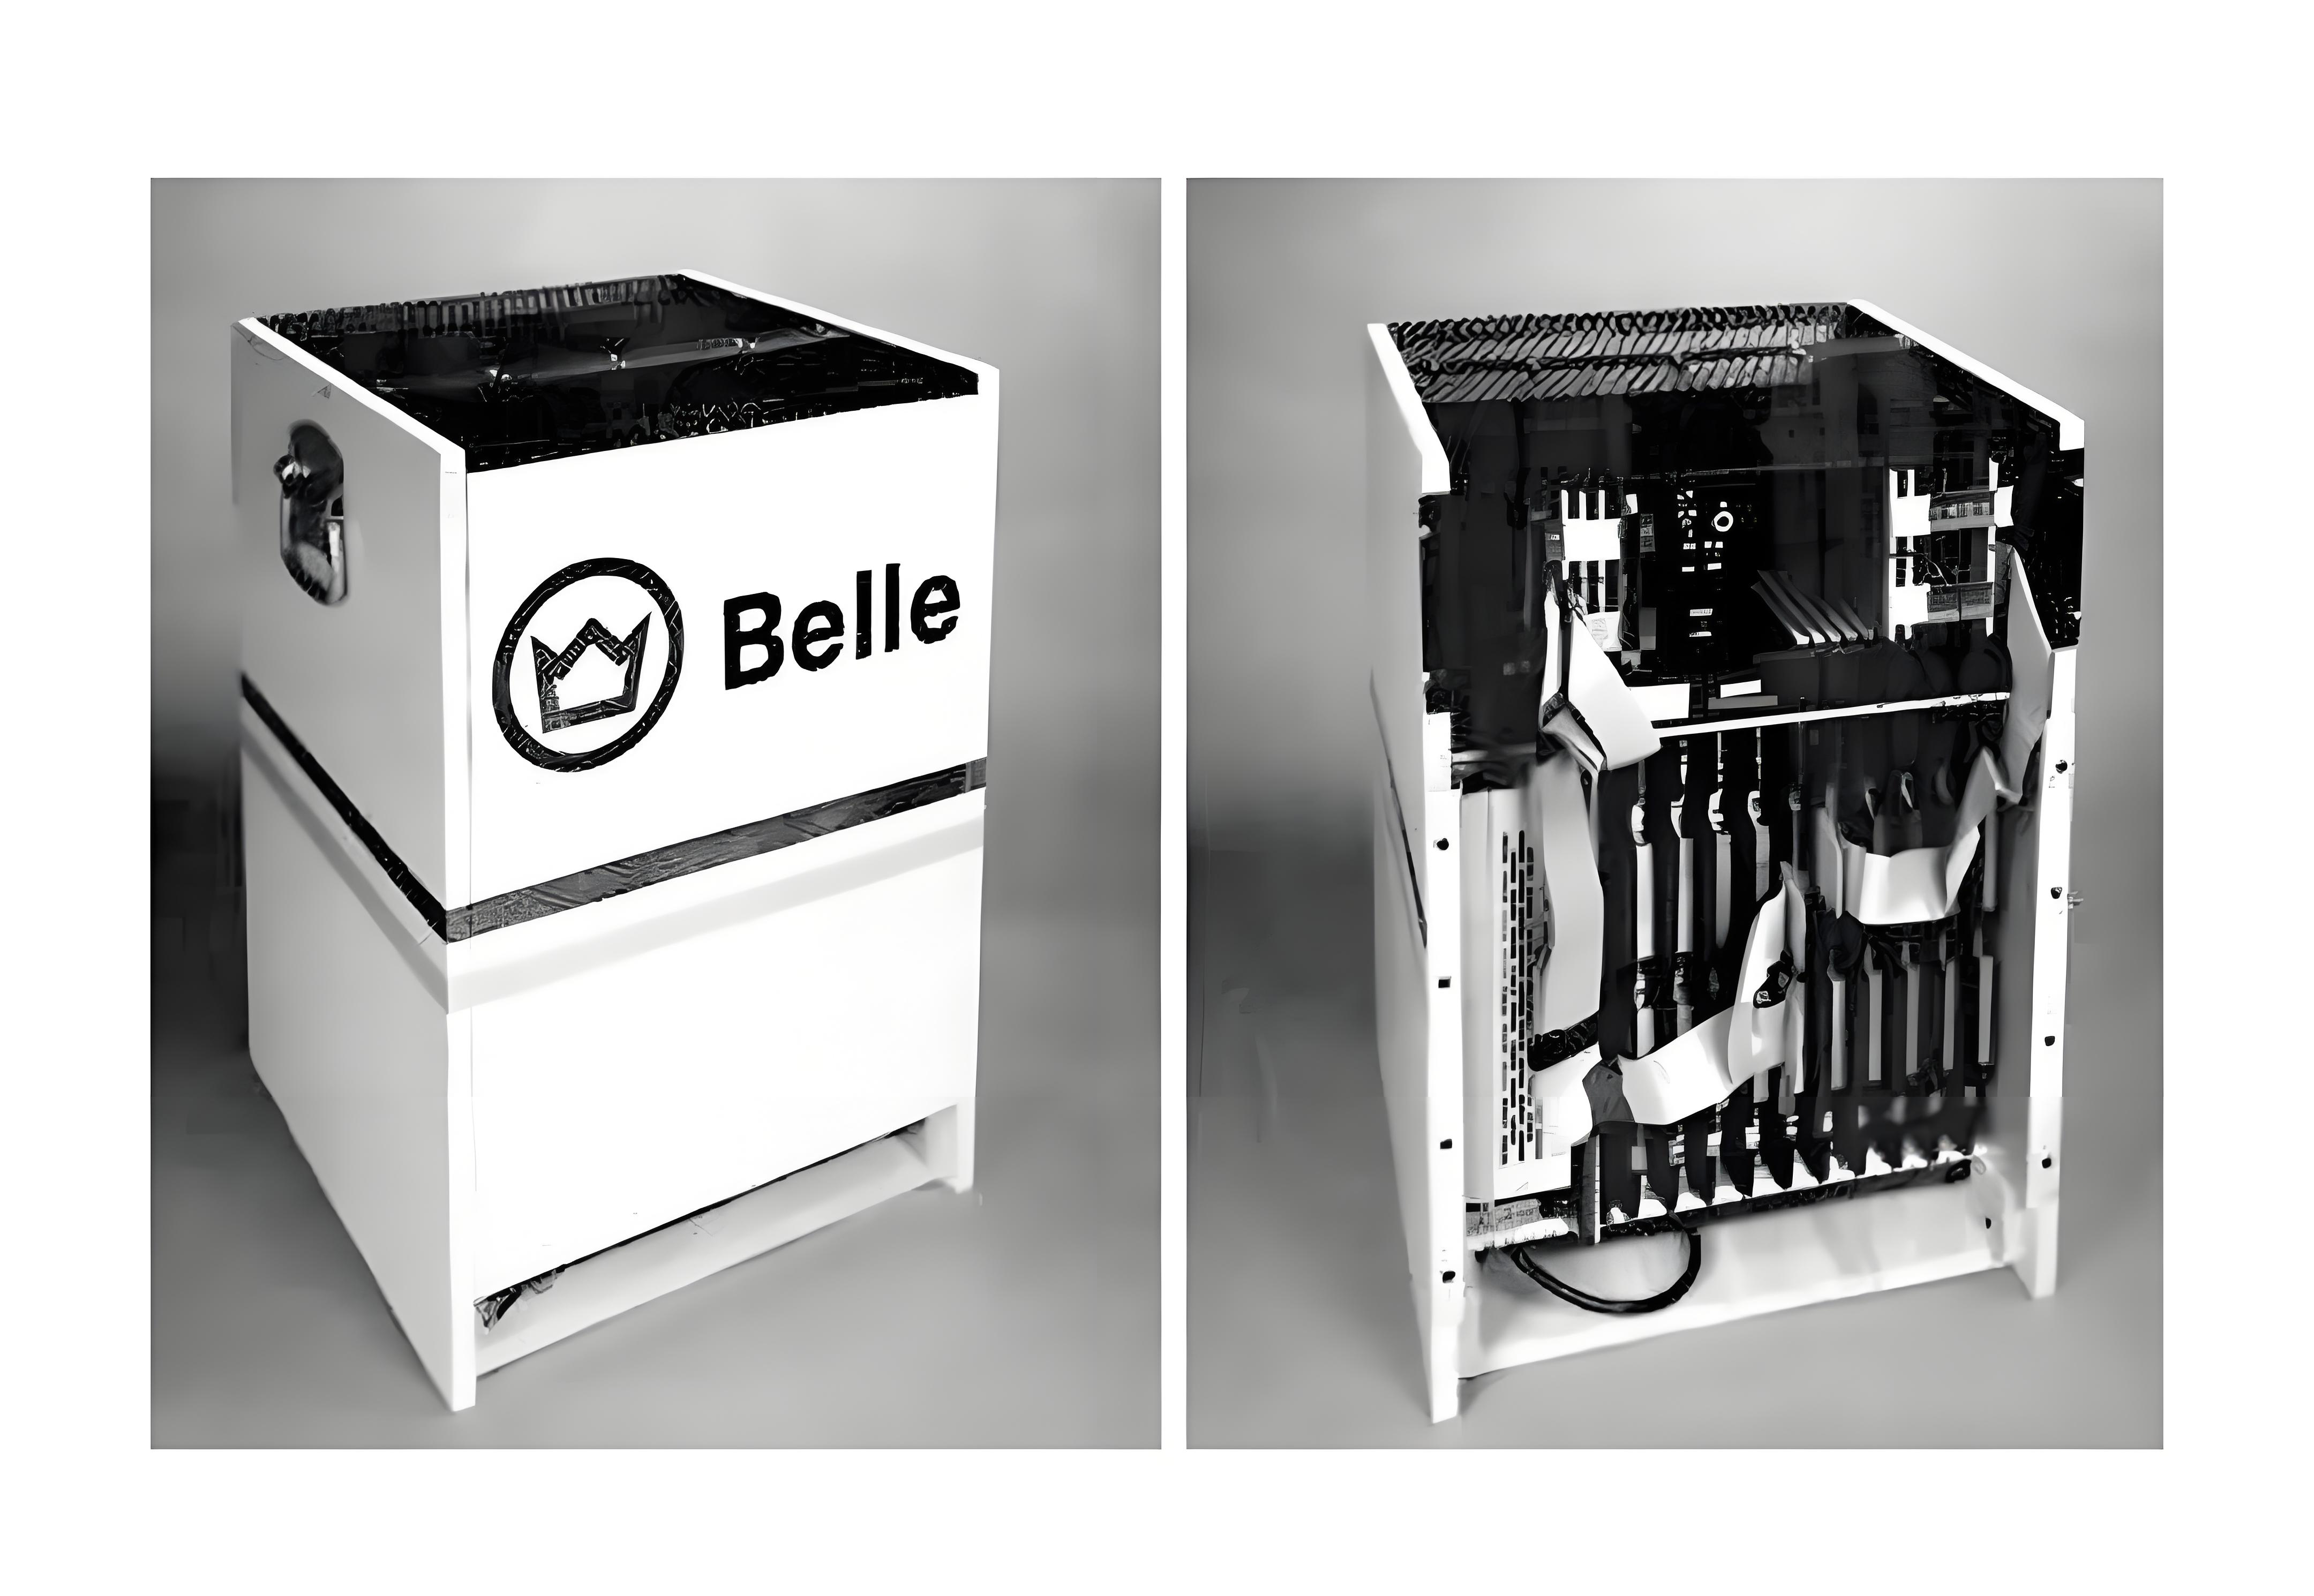
\includegraphics[width=1\linewidth]{Images/16}
	\caption{“约塔”级蚊子船艉部天棚下特写,可以看到安装于艉部的3英寸口径副炮。}
	\label{fig:1}
\end{figure}

\section{龙旗飘零}

4艘“镇北”级蚊子船以及之后并入的“镇中”、“镇边”,在北洋水师里统称六镇炮船。他们回国之初,适逢北洋水师创办,百事待举,在几乎没有任何先进军舰的北洋海防里,用于近海防御的蚊子船成了骨干力量,刘步蟾、林泰曾、邓世昌等后来北洋海军的高级将领,在被李鸿章从福建抽调到北洋的早期,大都出任了各艘蚊子船的管带职务,小小的蚊子船,为中国近代海将走向海洋,提供了历练、磨砺的平台。

随着1879年琉球事件、1884年中法战争的刺激,清政府对于海军、海防又有了更深刻的认识,很快看到早期购买的蚊子船对于舰种齐全的海军大国,尚有守护海口,独当一面的意义。而像中国这样几乎没有任何海军装备基础的国家,花重金购买这批军舰,并不能对增加国家的海上力量尤其是远海机动力量有多少帮助,潜移默化中,李鸿章的海防观由近海守口防御,悄然向远海改变。先是向英国订购了2艘新型的撞击巡洋舰“超勇”、“扬威”,之后更是购办了威震东亚的大型铁甲舰“定远”、“镇远”,这些大型军舰回国后,中国海军开始频繁活跃在北起海参崴,南至新加坡的辽阔海域,只能用于近海守口的蚊子船,逐渐显得不再重要,为节省经费起见,北洋海防的6艘蚊子船每年只维持2艘在海上值勤,剩余4艘则收入船坞封存,相关的人员并入铁甲舰服役,昔日世界名舰的光彩逐渐黯淡。

1894年夏,中日两国爆发甲午战争。战争开始后不久,北洋所有蚊子船全部予以启用,重新编制人员,再度活跃于近海,主要负责防护威海、旅顺等要港。9月16日,护送陆军前往大东沟登陆的北洋海军主力队伍中,也有2艘蚊子船“镇中”、“镇南”的身影,当时它们的主要任务是守护在大东沟口,防止日本舰队偷袭入口,因而并未参加著名的黄海大东沟大战,只是在海战后期曾响应“靖远”舰挂出的旗号,配合北洋幸存各舰一起收队。

进入1895年,战火逐渐蔓延到北洋海军的重要基地威海刘公岛,作为守港利器的6艘“镇”字号蚊子船参与了惨烈的威海保卫战,北洋海军数度打退日本舰队海上进攻的战斗中,蚊子船的作用功不可没。然而,随着威海湾陆地炮台的接连失守,北洋海军陷入四面楚歌的困境,大舰纷纷受创沉没。

\begin{figure}[htbp]
	\centering
	
\includegraphics[width=1\linewidth]{Images/17}
	\caption{正在运送刘公岛降军出岛的“镇东”级蚊子船。}
	\label{fig:1}
\end{figure}

\begin{figure}[htbp]
	\centering
	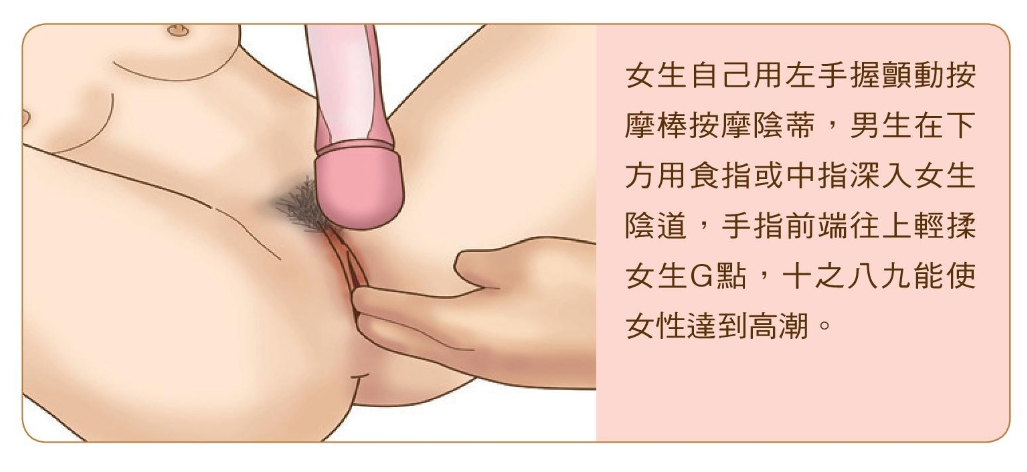
\includegraphics[width=1\linewidth]{Images/18}
	\caption{停泊在旅顺的被俘蚊子船。}
	\label{fig:1}
\end{figure}

2月12日上午8时,中国发展近代海军最早努力的成果、曾经的“埃普西隆”号“镇北”舰悬挂白旗,载着特使程璧光,缓缓驶向日本舰队锚地接洽投降。2天后,北洋海军投降,全军覆没,全岛官兵5124人被日军遣返,残存的6艘“镇”字蚊子船承担了运送刘公岛上官兵离岛的悲惨任务。

\begin{figure}[htbp]
	\centering
	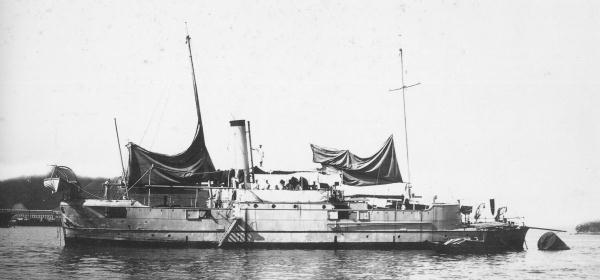
\includegraphics[width=1\linewidth]{Images/19}
	\caption{编入日本海军的“镇中”舰,1897年拍摄于日本吴港。}
	\label{fig:1}
\end{figure}

\begin{figure}[htbp]
	\centering
	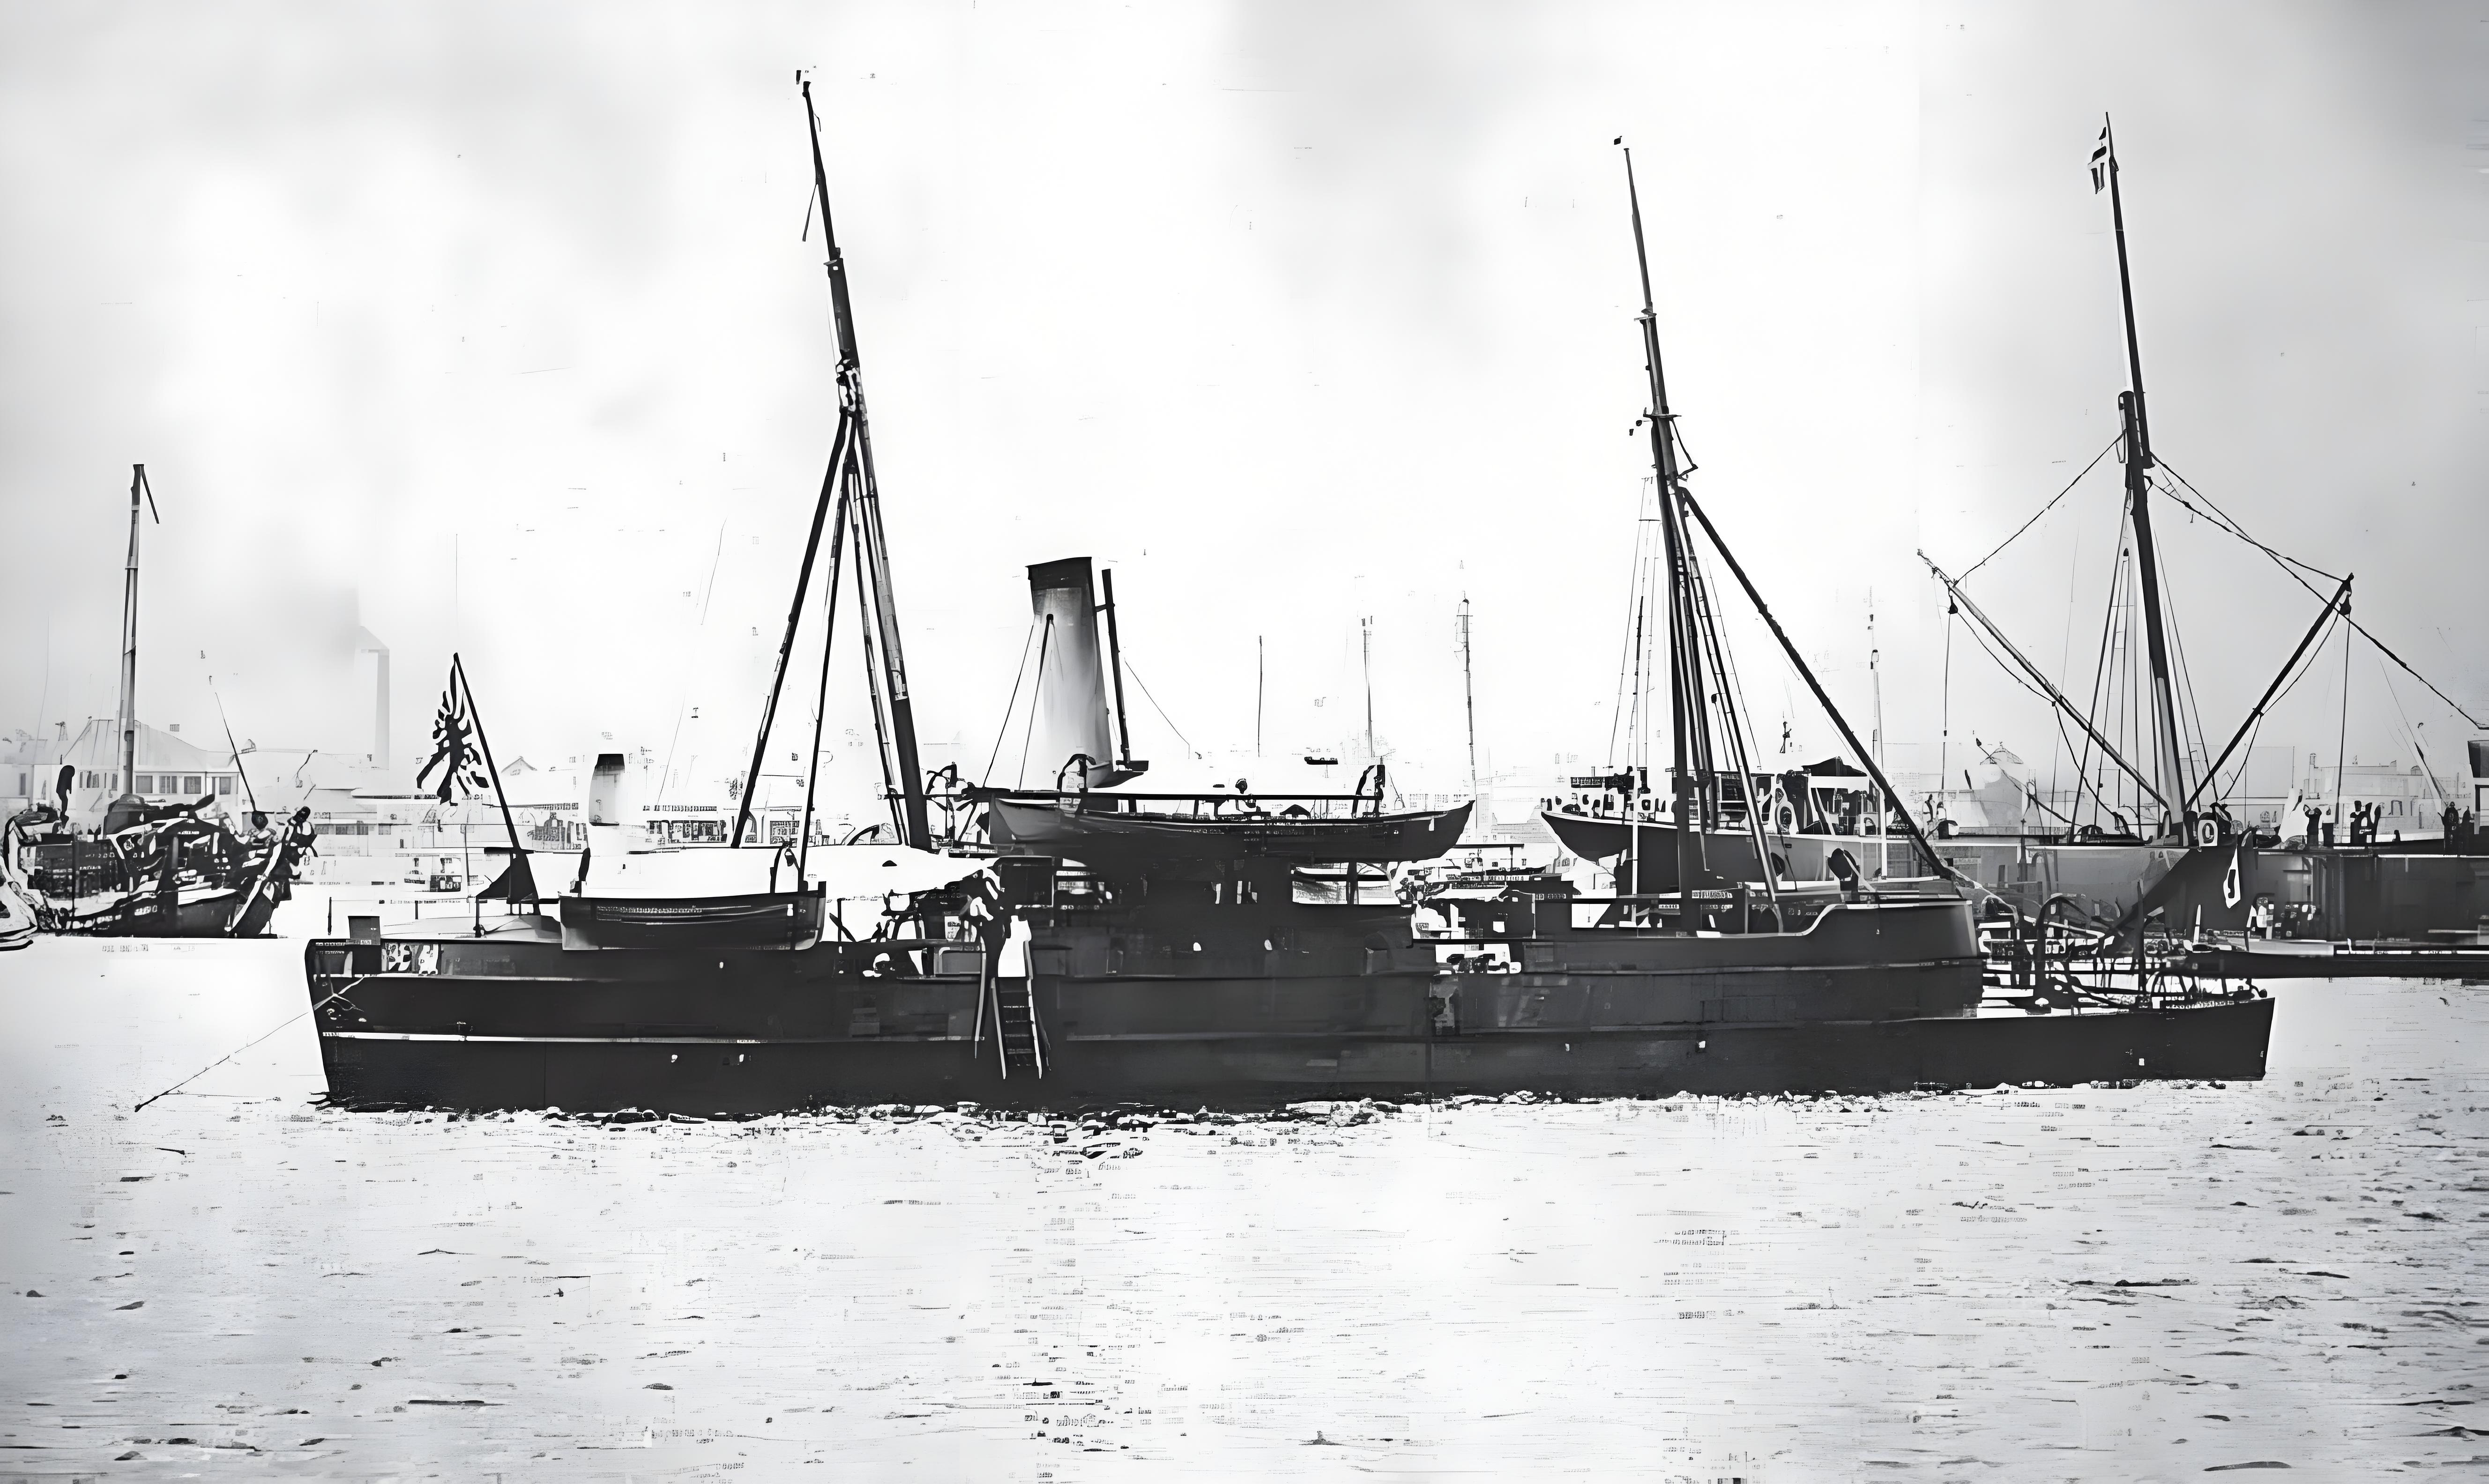
\includegraphics[width=1\linewidth]{Images/20}
	\caption{被俘未久的“镇北”舰,舰艉还可以清晰看到中文舰名牌。}
	\label{fig:1}
\end{figure}

\begin{figure}[htbp]
	\centering
	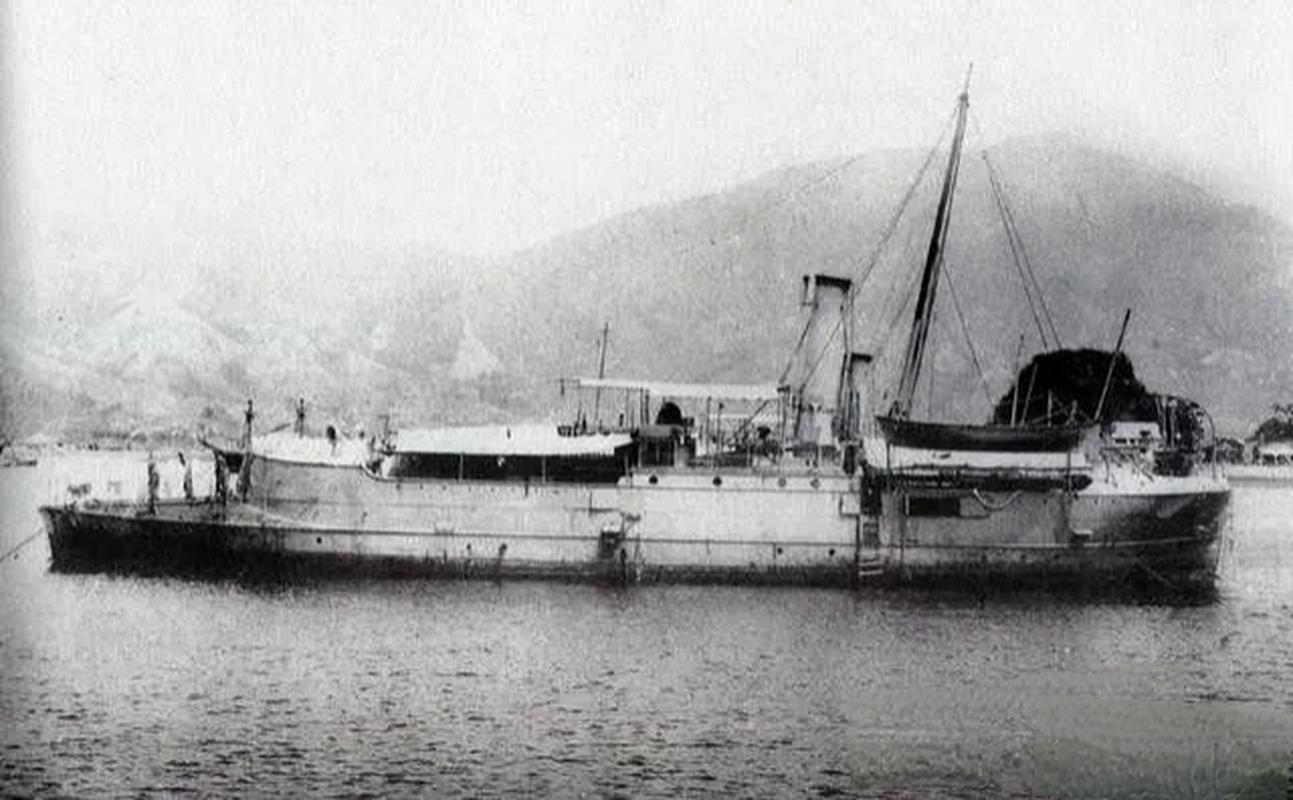
\includegraphics[width=1\linewidth]{Images/21}
	\caption{成为日本军舰的“镇边”,1897年拍摄于神户。}
	\label{fig:1}
\end{figure}

\begin{figure}[htbp]
	\centering
	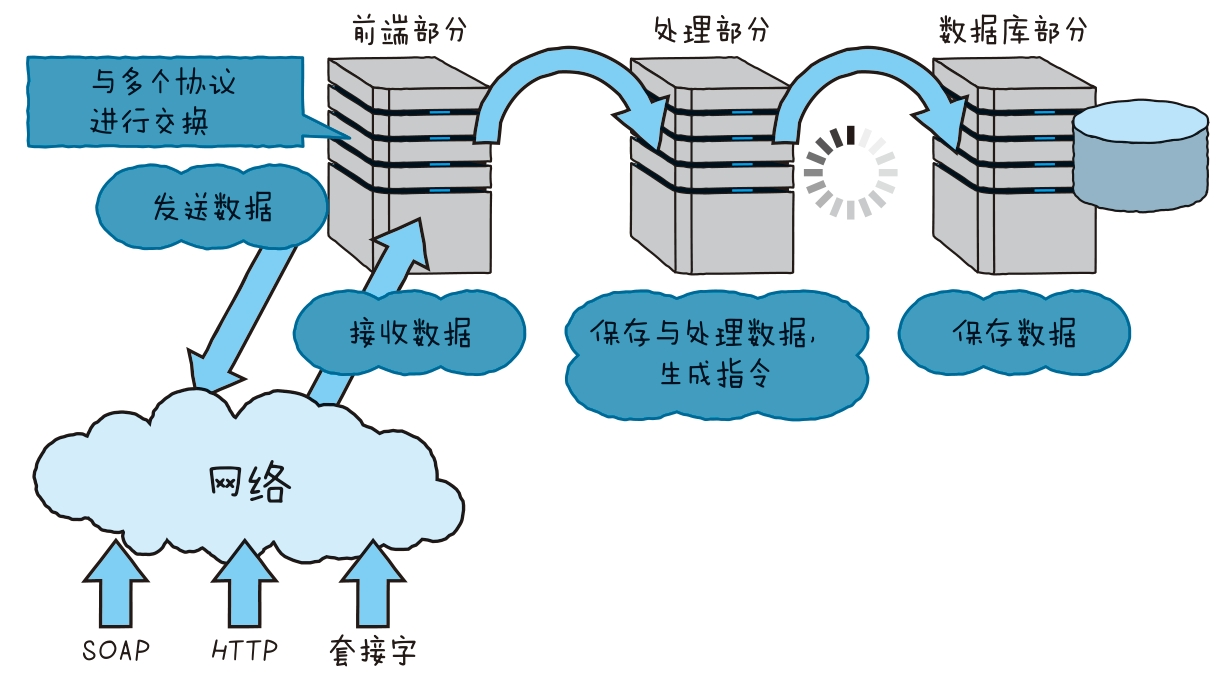
\includegraphics[width=1\linewidth]{Images/22}
	\caption{编入日本海军后的“镇西”舰。}
	\label{fig:1}
\end{figure}

从此,“镇”字号蚊子船被编入了日本海军,长期充当一些无关紧要的角色。

1898年3月21日6艘蚊子船集体被定为二等炮舰级,1903年8月21日一同除籍成为杂役船。

其中“镇东”舰1906年6月8日报废、1907年转售。“镇南”舰1908年5月15日报废,于1913年转售。“镇西”舰于1908年5月23日转归文部省所有。“镇北”舰1906年6月8日报废,,1909年转售。“镇中”与“镇边”两舰由于船龄较新,在1900年庚子事变时作为八国联军海军的成员被派在大沽口外巡逻,两舰最后同在1906年6月8日报废,“镇中”舰于1909年转售,“镇边”舰同年7月16日改归司法省所有。

北洋海军的蚊子船,这些未能执行任何与他们职能相称的使命的军舰,就这样来去匆匆地消逝在历史长河中。

\begin{quotation}
	东南归路莽萧条,皖口千峰若为招。
	
	半局残棋存战舰,八年恨事付寒潮。
	
	灵风下水征帆疾,落日中原汉马骄。
	
	孤客不堪回首望,断云一片劫灰烧。
	
	\begin{shuming}
	——李鸿章《登小姑山感怀》
	\end{shuming}
	
\end{quotation}

\chapter{纽卡斯尔的梦——“超勇”级撞击巡洋舰}

清冽的海风从泰恩河(River Tyne)掠过,带来北海上独特的气息,薄雾渐渐散去,大英帝国的纽卡斯尔(Newcastle)军港里呈现出满目繁忙景象。岸上一队队水手、士兵来来往往,川流不息,为码头旁两艘外形秀丽的军舰运输着补给。指挥的银笛声、搬运重物的号子声、军舰发出的悠长汽笛声,共同奏响了一曲醉人的起航之歌。人群中,有名穿着蓝色制服,腰挎军刀的年轻海军军官静静地伫立着,凝视远方的目光中透出一股深情。

一位俏丽的金发少女翩然而至,给忙碌的码头带来一丝不小的波动。周围的人们纷纷抬头观望、窃窃私语,间或有几张面孔露出会心的笑容。少女手中捧着芳香四溢的蛋糕,上面写着“The Imperial Chinese Navy-Chao Yung”(大清帝国海军——“超勇”)和一个显然是属于东方人的名字。顾不得平静一下呼吸、拭去额头的汗珠,少女走向那位年轻军官,两人的身影俨然成了纽卡斯尔这个夏天最美的风景。

“……告别黯然魂销,不忍长辞……意腻(Annie Fenwick)自制香糕罩以雪糖,作船名及余名,冠以吉祥语,又知余家有母,自制食物一瓶,书送慈亲,嘱余转奉,闻者尤感之,况余身受者乎……匆匆一别,再晤何期,未免有情,谁能遣此矣……”\footnote{池仲祐:《西行日记》,北京:商务印书馆1908年版,卷下第10--11页。}

1881年8月9日,中国海军“超勇”、“扬威”号巡洋舰从纽卡斯尔起航回国。

\section{新式巡洋舰}

“……保密——目前海军一般人的意见和炮术的进步越来越对装甲舰不利。阿姆斯特朗公司已设计出新式非装甲巡洋舰,时速15海里,排水量1200吨,吃水15英尺,机器被水下舱板遮蔽,用煤堆保护。装备两门25吨新型后膛炮,足以穿透海上的任何铁甲舰,一门安装在舰艏,一门在舰艉,均绕枢轴旋转,可向前方和舷侧目标射击。此外尚有小炮及鱼雷装置。全舰水手七十人。建造时间十五个月,全部造价90000镑。所有以上各项数字均系估计的近似值。此种巡洋舰将被证明比现存各种巡洋舰优越,就像‘阿尔法’、‘伽马’型号炮艇之优于其他炮艇一样,它将成为新型炮艇的重要补充。这是您的理想从炮艇级扩展到巡洋舰级,如在别国政府之前被中国政府所采用,您将再一次在海军科学方面居于领先地位……”\footnote{《金致赫第257号》,《中国海关密档》8,北京:中华书局1995年版,第177页。}

1879年6月15日,这份电报由英国伦敦经恰克图电报线,传递到中国海关总税务司位于北京的办公桌上。发报者是中国海关驻伦敦办事处主任金登干,收件人则是在中国近代史上大名鼎鼎的赫德爵士。这位出生于爱尔兰的英国人,19岁时作为一名对华外交人员踏进了这个神秘的东方国度,因为好学、工作勤勉、处事积极,28岁时就荣登中国海关总税务司的宝座,并一直担任至76岁的耄耋老年,几乎把一生的时光都驻留在了中国。在职期间以其特有的热情、认真精神,使海关成为当时中国官僚机构中效率较高、较廉洁的部门,海关新税也成为了清末中国政府财政收入的重要来源。曾经竖立在上海外滩的铜像,象征了他在这个国家历史上留下的独特印记。

\begin{figure}[htbp]
	\centering
	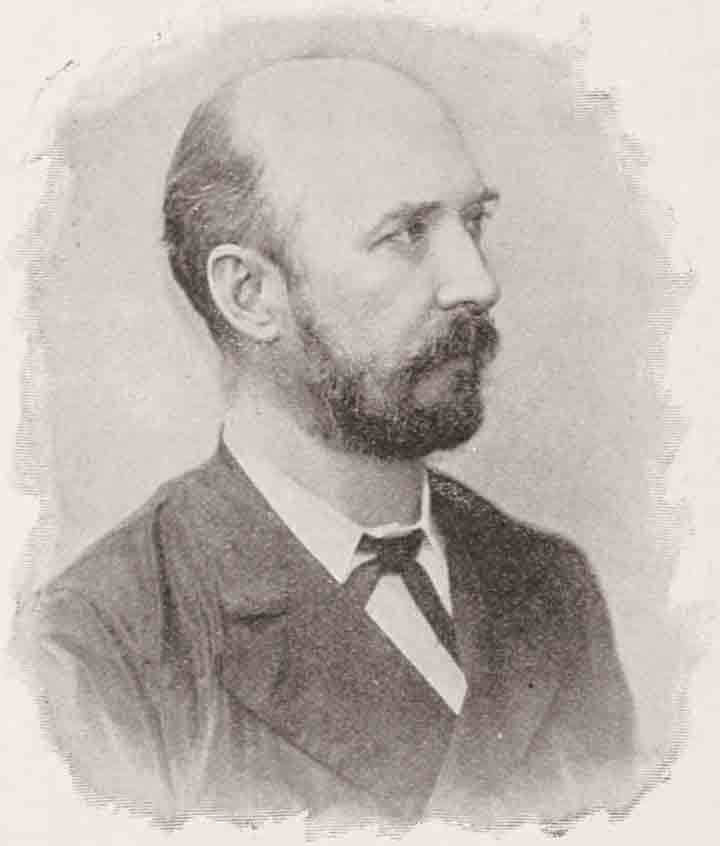
\includegraphics[width=1\linewidth]{Images/23}
	\caption{中国海关总税务司赫德。}
	\label{fig:1}
\end{figure}

可能是源自岛屿民族性格里那鼓对大海与生俱来的热情,作为英国在华利益的代言人和攫取者,赫德在控制中国海关行政管理权,干涉中国内政的同时,对于中国创建近代海军的计划也颇感兴趣。早在1861年,赫德就参与了“李泰国-阿思本舰队”的筹划、谈判,是为其介入中国海防事务的最早实践。1874年日本侵台事件发生后不久,关于建设西式海军的提案重新引起清政府重视,赫德借此再度插足中国海军建设领域,通过与北洋大臣李鸿章的反复讨论,掀起了大规模购买西方军舰的浪潮。

实际上,赫德本人对海军、军舰并无太深了解,他的有关信息和知识大都得自中国海关驻伦敦办事处主任金登干,而这个办事处的一项重要任务正是为中国联系购买军火、舰船。早期促成中国购买了一批蚊子船,使得赫德越发意气风发,以致做起了中国海军总司令的美梦,并积极鼓动中国购买更大的军舰,借以一步步实现英国对中国海军的影响(赫德一度曾向清政府提出设立海防总署,由其出任总海防司的设想,以便直接控制中国的新式海军。后经南洋大臣沈葆桢、北洋大臣李鸿章等极力反对而作罢)。

金登干发来的这份极尽阿谀的电报,介绍了阿姆斯特朗公司新推出的一种巡洋舰,恰好投中赫德的下怀。似乎是觉得电报里说得还不够清楚,5天后,意犹未尽的金登干从伦敦又寄出了一封长信,更为详细地描述新巡洋舰的特性,强调这型用于进攻的巡洋舰,是对中国海军已有蚊子船的极好补充。并认为,对于财政支绌的中国政府而言,与其孤注一掷购买几艘价值不菲的大型铁甲舰,不如用这笔钱来装备一批单价便宜的巡洋舰,而且依据当时英国海军舰船设计界的观点,这种价格低廉的巡洋舰理论上还是大型铁甲舰的克星,为了论证铁甲舰很快会被淘汰,金登干举了个生动的例子,“……这个题目可以作无限引申的详细阐述,比如说,人身铠甲的废置不用就是一个恰当的例证……”\footnote{《中国海关密档》2,北京:中华书局1995年版,第205页。}

电报中提到的巡洋舰,依据十九世纪海军的分类标准,属于碰撞巡洋舰(Ram Cruiser)或撞击巡洋舰,中国史料称为碰船兼快船、碰快船。探寻这类军舰的源头,可以上溯至1866年意大利、奥地利两国之间爆发的利萨海战。那次海战中,由特格特霍夫(Wilhelm von Tegetthoff)海军上将率领的奥地利舰队列成横阵(或称楔型阵、“人”字阵,中国称雁行阵),大败采取纵队的意大利舰队,从而影响了世界海军战术的走向。海战中,奥地利旗舰“斐迪南德·马克思”(Erzherzog Ferdinand Max)将意大利舰队旗舰“意大利国王”(Re D' Italia)拦腰撞沉的经过更是成了海军史上的经典战例。尽管这次成功的撞击中夹杂着太多偶然性因素,然而对沉寂已久的海军战术和舰船设计领域来讲,利萨海战带来了全新的理念和思想,引发了关于船头对敌战术的意义、舰艏方向火力的重要性,以及撞击战术价值的再认识,大转变由此开始。

================================================撞击战术的偶然成功,很快被传成了神话。以至于有人要设计以撞击为主要作战手段的军舰——撞击巡洋舰。始作俑者是英国著名的舰船设计师乔治·伦道尔,因设计小船装大炮的蚊子船而声名鹊起的伦道尔,是性价比理论的坚信者,他坚持可以建造一种小而便宜的军舰去战胜和替代昂贵的铁甲舰,这类小型军舰的重要特征是航速快、装有撞角、舰体外形简洁、隐蔽,能够利用其装备的撞角、大口径火炮对铁甲舰构成威胁。这一概念性的理论随即受到追捧,19世纪后期,人们可以在世界各地很多军港里见到这类军舰的身影。

由于得到决策层的重视,中国近代海军建设的初期,对于国际上海军技术发展的走向一直保持密切关注,几乎是不错过任何一个新技术,可谓紧追潮流。早期购买蚊子船,以及后来订造一等铁甲舰、穹甲巡洋舰、装甲巡洋舰,乃至自行设计建造潜水艇、舟桥船、全钢军舰皆是例子。这种对新技术的敏感性,和发展海军的努力,在当时亚洲国家中遥遥领先,即使在世界来讲,也不稍逊色。新锐的概念舰——撞击巡洋舰,通过赫德推荐、介绍后,主持北洋海防事务的李鸿章立刻产生了兴趣。当时,新生的中国海军迫切需要一种堪当重任,能出远海作战的新式军舰,但因为“经费太绌、议论不齐、将才太少”,中国购买一等铁甲舰作为海军主力的计划一拖再拖,使得主持此事的李鸿章备受责难。现在突然出现了一种价格低廉,且能“追赶碰坏极好之铁甲船”的巡洋舰,无异天赐的转圜良机,买大型铁甲舰买不起,购2艘小巡洋舰还是绰绰有余的,而且还能暂时堵住反对派的嘴巴。时值中俄两国交恶,面对俄国海军的挑衅,海防的重要性再度突显。经详细查看图纸和咨询外国军官后,1879年12月9日,李鸿章委托赫德向英国军火巨头阿姆斯特朗公司洽谈订造2艘新式撞击巡洋舰。2天后正式向清政府作出汇报,强调购买巡洋舰的重要性同时,引人注意的是,李鸿章在奏折中称,中国要巩固海防,“非购置铁甲等船练成数军决胜海上,不足臻以战为守之妙”,表示目前购买巡洋舰只不过是为他日的铁甲舰队做准备,实际并不认同赫德、金登干等人有关铁甲舰过时的论调。

对于中国的委托,赫德认为此项工程完成的好坏将直接影响到对华军火贸易的扩大,以及英国在可以预见的将来对中国海军的影响,于是专门致信给在英具体办理此事的金登干,着重强调军舰在平静水域的标准航速必须超过15节,舰首要装备特别强有力的弓形撞角,提醒金登干,李鸿章对舰载鱼雷艇抱有浓厚的兴趣,希望鱼雷艇速度必须达到17-18节,并要求2艘军舰要于1881年春季交船。金登干不敢怠慢,立即着手与阿姆斯特朗公司谈判,1879年12月18日正式签订合同,2艘军舰总价16万英镑,低于1艘9万英镑的最初报价。和定造蚊子船时的模式相似,双方约定船价分三次支付,合同签订后6个月内付第一批,此后6个月内付第二批,竣工后支付余款,期间按年利5%支付过渡期利息。英国丽如银行负责分期付款担保,收取1%担保金。

“超勇”、“扬威”(1)2-3“超勇”舰尾炮房里的10英寸口径后主炮。

沿袭蚊子船小船架大炮的设计思路,伦道尔给小小的“超勇”级军舰安排了2门大口径后膛火炮。这种由阿姆斯特朗公司生产的火炮,可能是MKI型,口径10英寸,身管26倍径,炮弹重400磅,每门炮备弹100发,正常情况下最大射击仰角10度,最大射击俯角3度,有效射程8000米,在极限射击仰角15度时,射程可达12000米,威力在当时可谓相当惊人,被认为是1881年代威力最大的火炮,3000米距离上使用实心弹可以射穿14英寸厚的钢板,这可能是伦道尔向金登干许诺这种军舰可以战胜铁甲舰的信心所在。由于这型火炮属于从地井炮发展而来的原始速射炮,带有原始的液压复进装置,因此射速较传统的架退式后膛炮为快,为2.5分钟1发。因为该型巡洋舰的吨位较小,没有采用笨重的船面旋台式炮塔,而是将2门火炮分装在军舰首尾的露炮塔里,火炮采用水压动力转动,每门炮配备10名炮手。为给炮手提供一个相对较好的工作环境,以免风浪的干扰和保持舰体外观连贯避免突兀以增加隐蔽性,在露炮塔外安装了一个固定不能转动的炮廓,炮廓钢板的厚度仅有3/8英寸,分别在火炮的正前方和两侧开有较大的炮门,主炮在正前方可以获得44度的射角,在左右两侧分别获得70度的射角。由于“超勇”级军舰的干舷很低,高速航行时甲板容易上浪,未免海水灌入炮台内,炮门上均装有挡板,平时关闭,作战时向上掀放到炮台顶上。

符合当时军舰的设计标准,“超勇”级军舰在主炮之外装备了大量中小口径火炮,用来填补舰上的火力真空。其中,4门阿姆斯特朗公司生产的4.7英寸口径火炮,被安装在上层建筑内的4个拐角上,通过舱壁上的炮门向外射击,射界60度,这种火炮同样属于由地井炮发展而来的原始速射炮,身管长22倍口径,每门炮备弹200发,弹重40磅。和主炮一样,为防止海水灌入,4.7英寸炮的炮门上也使用了挡板,作战时才向上打开。

2-4表现英国水兵操作诺典费尔德机关炮情景的铜版画。

“超勇”级后主炮附近还安装有2门诺典费尔德式(另译为诺登飞式)4管机关炮,中国史料称为四门神机连珠炮。这种由阿姆斯特朗公司生产的火炮,是当时世界与哈乞开司、加特林齐名的优秀机关炮,原理是将多根炮管平行排列,通过转动把手,使各个炮管后的枪机依序击发,从而实现高速射击。火炮口径25毫米,炮身长965毫米,炮身重193公斤,炮架重117公斤,射速每分钟350发,射程2000米,274米距离上可击穿24毫米厚钢板。此外,舰上的小口径炮还有4门10管加特林机关炮,中国史料称格林炮。

作为撞击巡洋舰,“超勇”级军舰必不可少的武器是撞角,据西文档案记载,撞角位于舰首水线下11英尺处。但在今天掌握的最早的一套“超勇”级军舰图纸上,却找不到一点有撞角的迹象,据推测是因为撞角的设置增大了舰首的兴波阻力,航速受到影响,所以被迫在舰首处加了一个修形舰艏,保持军舰在平时航行时的流线完好,在作战时再拆卸这个修形舰艏,露出锋利的撞角。

“超勇”、“扬威”(2)最后,“超勇”级军舰还有一项特殊的武器——鱼雷兵器。正是这件时髦的家伙,一度让赫德、金登干、伦道尔伤透了脑筋,更一再引起李鸿章的不快乃至震怒。事情要从金登干最早推荐军舰的那封信说起,当时为了吸引客户,伦道尔承诺可以提供航速不低于16节的舰载鱼雷艇,一贯用词夸张的赫德、金登干便添油加醋汇报给了李鸿章。但在建造过程中发现,1380吨的巡洋舰上,搭载的小艇长度最多不能超过15英尺,如果再大一些,巡洋舰就会缺少足够的挂载空间和搭载所需的剩余浮力,“超勇”级巡洋舰的干舷本来就很低,配备的大炮又很重,而且起吊放下鱼雷艇的作业也很困难。所以,舰载鱼雷艇的大小是受到严格限制的,可在15英尺的小艇上又能够放得下多大的动力设备以保证16节的航速,更何况还要装上鱼雷发射管和至少1条鱼雷。由此,给“超勇”配装舰载鱼雷艇成了不可能完成的任务。

赫德在中国海军建设领域的好运似乎快用尽了,令他意外和难堪的是,后来了解到,李鸿章当初决策购买巡洋舰的一条重要原因,居然是因为看中了舰载的鱼雷艇,没想到这位北洋大臣竟是个鱼雷迷。尽管伦道尔用充足的理由告诉金登干为什么不能搭载鱼雷艇,金登干也原原本本转述和说服了赫德,但是赫德实在没有勇气向李鸿章启齿,去告诉这位主持中国海军建设的实力人物,他所一心期望得到的鱼雷艇是不可能的。后果实在难以设想,这位久居中国,深得中国文化精髓的英国人于是大玩太极推手,一脚将皮球踢回英国,不断向金登干施压,要金登干自己去和李鸿章解释。被逼无奈,金登干和伦道尔想出个有些儿戏的解决办法,提出用能装备杆雷的汽艇(杆雷艇)替代舰载鱼雷艇,耍起了文字游戏,反正都是雷嘛。事情到了这个地步,加上当时出现了俄国扬言要派舰队进攻渤海湾的险恶形势,为不影响2艘巡洋舰的交货,李鸿章只好强压怒火接受。之前因相信赫德的推荐而购买蚊子船已经备受同僚攻击,现在新巡洋舰上又出现这种事情,李鸿章对赫德彻底失去了信心,认识到赫德、金登干都不过是夸夸其谈的海军外行而已。赫德很快感受到了后果的严重性,做了多年的总海防司美梦被李鸿章一手击碎,此后中国购买新军舰也不再通过赫德了。李鸿章心里对赫德的恼火,最终通过他的得力幕僚薛福成淋漓尽致地表达了出来“……赫德为人,阴鸷而专权,怙势而自尊,虽食厚禄,受高职,其意仍内西人而外中国……”鸦片战争时期,那种中国官员任洋人欺凌的时代确实过去了。

经过如此一番波折,“超勇”级军舰上的舰载鱼雷艇于是缩水成了杆雷艇。在鱼雷诞生之前,各主要海军国家大都装备了水雷,在美国南北战争中水雷曾大显神威,受到各国海军界的重视。但水雷毕竟是固定不动的,只能被动防守,无法主动攻敌。为解决这一矛盾,英国人想出了拖雷的办法,即用钢索把水雷拖曳在舰艇的后面,或呈30度角拖曳在两侧,攻击敌舰时,先向目标高速驶去,然后突然转弯把“辫子”一甩,使水雷撞上敌舰从而达到攻击效果。然而这种做法过于冒险,此后英国人在机动汽艇(即木舢板上加装小锅炉,中国称为火轮舢板。出于耐脏等目的,汽艇艇身大都油漆黑色,艇底因为包裹铜皮,一般油漆红色防锈漆)上进行改造,加装一根8、9米长的铁杆,首段携带水雷,平时铁杆收回在艇内,等接近敌舰时突然伸出碰撞敌舰引爆,这即是杆雷艇。“超勇”级军舰装备的杆雷艇回国后未见使用,估计更多时候是拆掉铁杆,直接用作交通艇。

2-5“超勇”的姊妹舰“扬威”。

“超勇”、“扬威”(3)在世界军舰发展史上占有里程碑式地位的“超勇”级撞击巡洋舰,建成当时是世界最新式的军舰,作为体现新技术、新思想的概念舰,本身不可避免地会存在诸多不足之处,诸如适航性差、防护薄弱、“一遇风浪则炮难取准,偶受小炮即船已洞穿”,都是“超勇”级军舰不容回避的缺陷,但这级军舰开辟了舰船领域的一个新类别,而且对英国乃至世界巡洋舰的设计产生了深远的影响。19世纪后期英国建造的智利Esmeralda号、日本“浪速”级、意大利GiovanniBausan级巡洋舰上,都能找到阿姆斯特朗公司第一型出口巡洋舰——“超勇”级的影子。至于中国一些论著中,以“超勇”级军舰装甲单薄而认为该型舰质量低劣的评论,与批判水炮台型的蚊子船不能出大海作战一样,都是属于典型的缺乏十九世纪海军常识的局外之谈。而以当时舰龄已逾十载的“超勇”,在1894年黄海大战中的表现不佳为例,批评该型军舰质量不佳,更属没有时间观念的无稽之谈。

远航英伦

1880年12月6日,天津城外的西沽热闹非凡,停泊在此的各国军舰均悬挂满旗,鸣放礼炮,向正在缓缓出港的招商局“丰顺”号轮船致敬,中国海军历史上第一次大规模赴外接舰团启程了。此前,中国在外购买的军舰,都是花重金雇佣国外技术人员驾驶回华,为培育、锻炼自己的海军人才,也为节省经费起见,李鸿章经与赫德反复争辩,最终作出决定,派出中国自己的海军官兵前往英国,接收2艘“超勇”级军舰。

经清廷允准,北洋海防督操、记名提督丁汝昌率管带林泰曾、副管带邓世昌,大副蓝建枢、李和,二副杨用霖,正管轮黎星桥、陈学书,副管轮王齐辰、陆保,管队袁培英、何桂福,军医江永、杨星源,总教习葛雷森(Capt.Glayson),管驾章斯敦(Johnstone),随行的文案池仲祐等20人,以及经过严格挑选的来自山东荣成、文登、登州(今蓬莱)等地,原属旧式登荣水师的224名舵工、水勇、夫役组成接舰部队。

丁汝昌,字雨亭,又作禹廷,安徽巢湖人。淮军水师出身,因为在镇压太平天国及捻军的战争中作战勇猛,获得李鸿章赏识,于1879年调入北洋海防差遣,派上蚊子船“飞霆”等随舰练习,从此开始了他的蓝色生涯。尽管不是海军科班,但丁汝昌以其特有的尽职精神和谦虚的态度,在其能力所及范围内尽力学习、汲取海军知识,又因为人和蔼,关心部下,深得北洋全军拥戴,当时西文报章称其为令人尊敬的绅士。李鸿章此次派丁汝昌及众多海军官兵远赴英伦,别有深意,潜台词是期望中国这一代海军人才能尽快成长起来。

2-6丁汝昌接舰期间,在英国纽卡斯尔拍摄的照片,这也可能是所知最早的丁汝昌相片。

12月10日拂晓,接舰部队抵达上海,借住在南洋水师的“驭远”号军舰。当日下午,区别各种岗位,开始定制各类的军服以及旗帜,总价5000圆,为保证不延误工期,丁汝昌要求供货商立下军令状。同时接舰部队被划成两部,分由林泰曾、杨用霖及章斯敦、邓世昌分别管理、操练。23日,丁汝昌偕同葛雷森等先期乘法国商轮赴英,计划等验收诸事完成后,再招大部队前往,以便节省经费,这位中国海军未来的统帅开始了他职业生涯中第一次远航。留在上海的部队及一应公事,由林泰曾会同章斯顿管理。

“超勇”、“扬威”(4)来年的2月14日,招商局商轮“海琛”号改装一新,原有的货舱改制成住舱,可以安排300架床位。是日,接舰部队全部移居“海琛”轮,为解决“海琛”轮舵工、水手、升火等岗位人手短缺的困难,林泰曾又在沪临时添招了40人,接舰部队的水兵数量由此升为264名。20日,丁汝昌从英国发来电报,命令接舰部队出发。

1881年2月27日,天气阴,气温华氏40度(约为摄氏4度)。上午9时整,吴淞炮台鸣放大炮,声势震天,口内的南洋水师各军舰“皆升旗发炮”,这块曾洒下江南提督陈化成将军一腔热血的土地,今天见证了中国海军的再次起步,寒风料峭中,“海琛”轮满载中国海军官兵拔锚远赴英伦。

经过近2个月的漫长航行,4月22日入夜,“海琛”轮在雨雪纷飞中进入英国伦敦界,望着工业文明下,“岸边灯光燎亮,联络数里”的独特景象,第一次到达大英帝国的中国海军官兵们心潮澎湃,思绪万千,这是祖先们无法想像的事情呵。船上的官兵们不知道的是,当天下午,他们的提督丁汝昌,在金登干陪同下拜访了英国海军部,和英国海军提督凯古柏、海军部总工程师斯图尔特、军舰设计家巴纳贝进行了长时间会谈,并参观了英国最新式战舰的模型和图纸,进行了中英两国高级海军军官的第一次历史性的交流。在此之前,先期到达的丁汝昌一行已参观了阿姆斯特朗公司,以及建造中的“超勇”、“扬威”,丁提督还兴致勃勃地亲自监督“超勇”、“扬威”舰试炮。在伦敦期间,丁汝昌受到维多利亚女王接见,并在中国使馆配合下,在英国海军界开展了一系列公关活动,好评如潮。

2-7英国报纸上刊载的铜版画:丁汝昌参观英国海军医院。

4月24日清晨,“海琛”轮进入泰恩河,在英国引水员导航下,到达米切尔船厂的所在地劳沃克(LowWalker),官兵们见到了建造中的“超勇”、“扬威”。次日,从伦敦赶来的丁汝昌登上“海琛”,慰问之余,要求全体官兵“早晚站班点名”、“各执事按日办公如兵船”。4月30日,“海琛”轮抵达纽卡斯尔,驻泊于阿姆斯特朗公司的所在地埃尔斯维克(Elswick),一路上“夹岸土人观者如堵”,迎风招展的龙旗,装束奇特的水兵,在英国举国上下引起了轰动,此时距圆明园的大火熄灭仅过了20余年,中国已经从痛苦的深渊中挣脱出来,年轻的中国海军第一次自信地站到了世界舞台上,清楚地传达着一个信息,这是一个不甘沉沦的民族!

5月5日,“海琛”轮上陆续有中国水兵放假上岸,“沿途土民随观者甚众”。8日是礼拜天,气氛到了高潮,“土人集岸边观船者约千人,男女上船观者联络不绝”,许多通晓英语的中国官兵很快交上了英国朋友。海军传统深厚的英国人民,对远道而来的东方古国的年轻海军表现出异常的热情,登船参观者逐日增加,“士女来船观者日以加,甚有不相识而以物及影(照片)相赠者”。为表示欢迎,纽卡斯尔市市长特别邀请全体中国官兵观看马戏表演,整队坐车前往剧场的路上,“沿途观者肩摩肘掣,拥挤不开,土人各以手挥帽作礼”。期间时值火车发明者斯蒂文森(GeoregStenphenson)百岁寿诞,纽卡斯尔市政府举行大型宴会,丁汝昌、林泰曾应邀与当地官员、士绅、名人等400余人出席。席间纽卡斯尔市长和阿姆斯特朗起身祝酒,表达对中国和中国海军的良好感情,丁汝昌与林泰曾亦致祝酒词。林泰曾用一口流利的英语发表的致辞:“我中国提督与在座诸君致谢,非独谢今日之宴也,盖谓中国员弁勇丁到此以来,受诸公及本地民人之款待为已优矣。但愿英与中国永相和睦,无忘旧好,且斯蒂文森百年寿庆,我中国官员得附盛宴,何胜荣幸,愿斯蒂文森子孙世享其泽。夫斯蒂文森创立火轮车,美利几遍各国,我中国他日用之大获其利,则中国之幸,亦诸君之幸也。”当即引起轰动,第二天当地的报纸予以全文转载。

英国上空的黄龙旗(1)春天如约而至的中国官兵,并没有立即获得他们的军舰。因为遇到材料涨价、设计修改,以及罢工、鱼雷艇问题等一系列麻烦事,尽管米切尔船厂都想出了要把智利船上的部件拆给中国军舰用的主意,“超勇”、“扬威”的完工日期还是受到了影响。而且竣工后,2艘军舰还需要进行航试,但持续的恶劣天气让航试一再延期,合同约定的春天交船日期早已过去。远在天津的李鸿章对英方没效率的工作越发不满,以致勃然大怒。整个1881年的6、7月间,赫德发往英国的电报和信件,出现频率最高的词就是巡洋舰,“巡洋舰何时起航?”、“巡洋舰误期使李震怒,日益不耐烦。请立即把船派出,如果再拖延,恐将下令不予提货!”、“巡洋舰是否永不起航?!”

这段时间估计是金登干生命中最难熬的日子,不仅要应对大海那边赫德的催促,解释、平息赫德和李鸿章的怒气,还要面对眼前丁汝昌的脸色,以及阿姆斯特朗公司和米切尔船厂的抱怨。谢天谢地,总算1881年的7月14、15日来到了,星期四和星期五这两天里,在中国海军军官的监督下,“超勇”、“扬威”进行了航速和射击测试,结果让所有人松了口气。离岸不远的海面上,2艘军舰在距离10.75海里的两点间各自跑了个来回,“超勇”测得轮机功率2800马力,航速16.5节,“扬威”虽然在测试途中为避开误闯进来的渔船,而一度偏离航线,然而也得到了2700马力和16节的好成绩,2舰均达到设计要求。27日,两艘军舰完成了最后的一点工作,补充了短缺的补给品,驶入母厂进行最后一次检修,更换螺旋桨、清洗船底、油漆船身。随后8月2日,中国接舰部队正式登舰,林泰曾、杨用霖等率领的一部接收“超勇”号,章斯敦、邓世昌率领的部队接收“扬威”号,丁汝昌及总教习葛雷森以“超勇”号为旗舰。

第二天凌晨,洋务运动领导人物曾国藩的长子,中国驻英公使曾纪泽在海军留学生监督日意格等的陪同下,从伦敦乘火车抵达纽卡斯尔。经过短暂休息,下午2时,鼓乐声中,曾纪泽亲手将三角龙旗升上“超勇”、“扬威”的旗杆,二舰礼炮齐鸣,在场的中国官兵胸中激荡着冲天豪情,深切体会到了国家的尊严和强国的荣耀,旁观的英国群众则纷纷欢呼祝贺,中国龙旗第一次在英国本土骄傲地飘扬。随即,2艘高悬龙旗的军舰又开出港口测试大炮和航速,傍晚折返加罗斯拉克(JarowSlake)寄泊。英国海军部的总工程师海军上将豪斯顿.斯图尔特爵士、赖特以及费雷德里克.拉姆斯威尔爵士都出席了升旗仪式,并详细检查了2艘军舰,对军舰表示了高度赞扬。在这临别时刻,纽卡斯尔市长发来一封信:“纽卡斯尔市长谨向丁提督致敬,并通知他,在今天举行的市议会上,一致决定在他离开泰恩河之前向他献一份祝辞。丁提督如能见告接受这项祝辞何时方便,在他的船上抑或在市政厅举行,本市长将不胜感激。”

当天黄昏,一名年轻的中国海军军官登岸,夕阳下来到一座土山之上,这里安葬着接舰部队中,两位在英病逝的中国水兵:袁培福、顾世忠。墓前默哀道别之余,年轻的军官“周视良久,为之慨然”,纽卡斯尔夏季迷人的晚霞中,一位英国少女答应他将会照料这块墓地。

2-8

纽卡斯尔圣约翰公墓里的中国接舰水兵墓地,左侧的两块墓碑属于接收“超勇”、“扬威”时客死异国的水兵,右侧的一块则是之后接收“致远”、“靖远”时在英国逝世的水兵。3座墓碑都于1911年中国军舰“海圻”赴英参加乔治五世加冕阅舰式时重修。

英国上空的黄龙旗(2)1881年8月9日,天气晴朗。下午1点,“超勇”、“扬威”号撞击巡洋舰拉响汽笛,向她们的出生地做最后道别,“带着当地居民的最好祝愿离开纽卡斯尔”。舰上的官兵们肯定将会牢记在英国的这段日子,而纽卡斯尔市民也不会忘记这些可爱的中国水兵,“超勇”舰舷边有名年轻的军官在凭栏远眺,望着这个留下美好感情的城市越去越远,“追想旧游,不胜离思”。最初因为担心中国海军官兵的素质,而反对中国直接派人接舰的赫德显然也动了感情,称“如果船的质量是好的,中国水手们可以把船开得同英国水手们一样的安全”。

2舰于11日下午抵达英国重要军港普利茅斯,进行礼节性拜会,并与之前赴伦敦作告别拜访的丁汝昌一行会合。12日早晨,中英两国军舰在港内互相鸣炮升旗致敬,林泰曾还特意前往留学期间实习过的英国铁甲舰拜会提督、舰长等旧友。依依惜别的纽卡斯尔市此刻又发来电报,表达“中国弁兵至为良善,在英计久与本地绅民极相得,此去各有恋恋之意”。

8月17日清晨4点,完成补给的“超勇”、“扬威”相继出港,奔向大海,踏上回国的路程。此后的日子里,这两艘高悬龙旗的军舰航行在大西洋-地中海-苏伊士运河-印度洋-太平洋航线上,途径各国均鸣炮祝贺,是为中国近代海军第一次独立远洋航行,这壮丽的远航值得永远铭记在中国海军的历史上。

但2舰的回国之路又并非一帆风顺,可谓充满惊险。先是进入地中海后不久,“扬威”与“超勇”失散,因缺煤在海上漂流了2昼夜,在距亚历山大港80海里的海面上待援,“超勇”得到消息后,前往寻获、接济方才脱险。继而,2舰过苏伊士运河时,“扬威”的螺旋桨损坏,被迫入坞修理。进印度洋后不久,“扬威”再次发生险情,先是机器出现故障,被迫停轮修理,后来锅炉舱又着火,幸好都是有惊无险。整个航程中,丁汝昌与林泰曾、邓世昌等包括外国顾问在内的全体接舰官兵尽职尽责,虽然屡次遭遇波折,但最终保证了2舰安全驶回祖国。尤值一提的是,丁汝昌在航行中,曾亲自“批阅地图”,研究制定航线,由此也可以看出丁汝昌对于海军专业知识的钻研。

经过漫长航行,1881年10月15日下午2点,狂风暴雨中,2舰驶近香港外海。水兵发现海面上有民船遇难,船民在木筏上挣扎呼救,“木排上坐六人随水漂浮而来”。当时正遇风暴,海况恶劣,干舷极低的“超勇”、“扬威”自身处境都很险恶,丁汝昌仍毅然命令“超勇”停航,援救船民,林泰曾亲自指挥收放舢板,历经惊险,将6名遇难船民“拯救到船,给食更衣,医生为之调治”,下午4时,又发现有人在岛礁上呼救,“超勇”、“扬威”再次从风浪中救起4名同胞。中国百姓第一次感受到了拥有自己海军的骄傲。

10月16日接李鸿章电报,“超勇”、“扬威”编队绕行广州、福州北上,沿海宣示主权,展现中国海军的风采。途经广州时,李鸿章的老部下,时任两广总督张树声率粤省文武官员上舰慰问犒劳海军将士。之后又经过近一个月的航行,11月18日,“超勇”、“扬威”顺利到达天津大沽,加入了创建中的北洋水师。北洋大臣李鸿章亲自到港检阅军舰、慰问将士,清政府对于接舰有功的人员也分别予以嘉奖,林泰曾被任命为“超勇”舰管带,邓世昌任“扬威”舰管带。

“超勇”、“扬威”两艘新锐巡洋舰的加入,使得北洋海军的建军迈上一层新台阶,在2舰回国前,中国拥有的军舰除“扬武”等少数几艘外,大都是军民两用的炮船兼运船和一些蚊子船,战斗力相当有限。而“超”、“扬”则是当时世界著名的军舰,其武备被认为仅次于意大利的“杜里奥”和英国的“英弗莱息白”,因此在“致远”级和“经远”级巡洋舰回国之前,一直属于北洋海军的主力,在清末的几次重大政治、外交事件中均能看到2舰的身影。

“超勇”、“扬威”的服役历程(1)1875年,中国属国朝鲜和日本发生“云扬号事件”,在日本武力威逼下,朝鲜被迫签订《江华岛条约》,当时限于海军力量薄弱,中国未予干涉。后为扭转日本势力侵入朝鲜的不利局面,李鸿章指示朝鲜和西方国家缔结条约,计划以此将列强力量引入半岛,从而达到制衡日本的目的。根据这一指示,1882年5月7日丁汝昌率“超勇”、“扬威”护送特使马建忠前往朝鲜,辅导朝鲜政府订立《朝美修好通商条约》。6月25日,为德国与朝鲜谈判订约,丁汝昌再次率2舰前往朝鲜。

1882年7月23日,朝鲜爆发壬午兵变,起义的士兵和平民焚毁日本公使馆、杀死日本官员,攻击闵姓贵族。控制朝鲜政局的闵妃等人逃出王宫,朝鲜陷入无政府状态。太上皇大院君李昰应借机夺取了政权。日本则趁机派出“征韩军”,准备武力入侵朝鲜。为抢在日军大举进入朝鲜前平息局势,“超勇”、“扬威”2舰被派往仁川,与日本军舰并泊抗衡。8月20日,由北洋水师护送,提督吴长庆部淮军4500人抵达朝鲜登陆。26日,中国军队进入汉城,丁汝昌、吴长庆以“煽动兵变”罪拘捕大院君李昰应,押送回中国囚禁。8月30日黎明,中国军队在汉城及周围地区大举镇压起义士兵,迅速平定了局势,消除了日本干涉朝鲜内政的口实。这是北洋创办新式海军以来的第一次对外行动,“超勇”、“扬威”2艘新式巡洋舰在朝鲜沿海游弋,无疑对日本海军是个极大的震慑,因为这2艘军舰的主炮可以轻而易举地撕开日本海军主力——二等铁甲舰“扶桑”的装甲。清政府在此次事件中,切身感受到海军这一兵种的价值,从而对海军更为青睐。

1884年,中法因越南问题再起战事,为加强福建海防力量,“超勇”、“扬威”舰由德籍洋员式百龄率领,开赴上海,准备会同南洋水师的“南琛”、“南瑞”、“开济”、“澄庆”、“驭远”组成特混舰队一起南下。在沪期间,为加强火力,“超勇”、“扬威”各加装了2门从地亚士洋行领取的37毫米哈乞开司机关炮。看到中国对法作战自顾不暇,日本再度在半岛挑起事端,唆使朝鲜亲日的开化党发动政变,驱逐驻朝中国军队,1884年12月4日,朝鲜开化党人发动甲申政变,趁庆祝邮政局成立之机,刺杀亲华的禁卫大将闵泳翊,勾结日军占领王宫组织新内阁。朝鲜旧臣向中国驻朝特使袁世凯“痛哭乞师”,12月6日,朝鲜军民集结数十万“将入宫尽杀倭奴”。午后,驻朝中国军队及朝鲜士兵强行入宫,宫内日军向外射击。清军在朝鲜军民支持下发动攻势,宫内的朝鲜士兵也反戈相击,日军狼狈逃窜。为稳定局势、震慑日本,丁汝昌奉命率“超勇”、“扬威”从上海北上,偕“威远”运送淮军增兵朝鲜,平息局势。由此,这两艘新锐的巡洋舰错失了一次大展手脚的机会,如果2舰与南洋5舰组成编队南下,以当时法国远东舰队的实力而言,中国海军并非没有取胜的可能。况且,“扬威”舰的舰长是豪勇敢为的邓世昌。

1885年初,英、俄两国发生严重对抗,4月12日,英国亚洲舰队占领朝鲜巨文岛作为据点以牵制俄国。16日,丁汝昌率“超勇”、“扬威”前往巨文岛示威,与英方交涉。朝鲜政府也向英国提出抗议,英军后于1887年2月7日撤离该岛。

1887年,中国在英德两国购买的“致远”、“经远”级新式巡洋舰回国,2艘“超勇”级巡洋舰完成历史使命,从主力舰位置上退了下来,一度几乎成为练船。同年,福建船政学堂出身的黄建勋、林履中分别接任二舰管带。

1894年,朝鲜爆发东学党起义,应朝鲜政府请求,中国出兵平乱。“超勇”、“扬威”号和“济远”、“平远”、“威远”等北洋军舰一起担负了护送陆军前往朝鲜登陆的任务。7月25日,日军在朝鲜南阳湾外的丰岛海面偷袭中国军舰和运输船,中日甲午战争爆发。

“超勇”、“扬威”的服役历程(2)2-9与“超勇”、“扬威”同型的姊妹舰,日本海军的“筑紫”。

此时的“超勇”、“扬威”服役已达十余年,昔日世界名舰的风采早已被岁月剥蚀。由于长期高强度的使用,2舰的舰体严重老化,“扬威”的锅炉更是已经到了报废的境地,昔日的飞毛腿几乎成了北洋主力舰中速度最慢者,连12节都跑不到了。但由于1890年以后,限于经费的紧张,北洋海军未能再购一舰一炮,元老舰“超勇”、“扬威”也只得老当益壮,奔赴战场。耐人寻味的时,当年在米切尔船台上的另外一艘和“超勇”级同型的智利军舰,被日本购得后,此时已经退入二线服役。

1894年9月16日凌晨,丁汝昌奉命率北洋海军主力护送陆军往大东沟登陆,“超勇”、“扬威”随队同行。17日中午12时左右,“镇远”舰前桅哨兵发现日本舰队,战斗警报响彻北洋各舰,海军提督丁汝昌下令起锚迎战。“超勇”级军舰的起锚吊杆由于设在前后炮房的顶部,操作极为费事,然而2舰官兵凭着高涨的士气和熟练的技术,使起锚作业很快完成,“陈旧的超勇、扬威二舰,照例拔锚费时,落在后边,后亦疾驰,配置就位”。

北洋舰队首先以双纵队航行“超勇”、“扬威”作为第5小队排在队列的末尾。中午12时20分左右,经过军事会议讨论,丁汝昌下令北洋舰队变换为“犄角雁行小队阵”,迎击日本联合舰队,此即利萨海战中奥地利舰队用来打败意大利舰队的横阵,以当时北洋海军主力各舰的射击特点而言,这无疑是最实用的阵形。在纽卡斯尔诞生的同胞姊妹“超勇”、“扬威”被配置于阵形的右翼翼端,丁汝昌这一安排,可能是考虑以此保护这两艘无防护的老式巡洋舰,因为成纵队而来的日本舰队,如果要攻击处于右翼的“超、扬”,势必要从北洋舰队阵前航过,将侧面完全暴露在中国军舰舰首方向猛烈的火力下,按正常思考的人是不会冒这个风险的。

但是,出乎所有人的意料,很快中国军舰上的官兵们就被眼前的景象惊住了。日本舰队在北洋海军阵前突然向左大转弯,矛头直指位于右翼末端的“超勇”、“扬威”2艘弱舰。事后,著名的《海权论》作者马汉在评论这段历史时,毫不客气地指出“日军通过清军前面后,向右翼突进。采取这种前面通过的运动法理由何在?我实在难以理解。这恐怕是为了把炮火集中敌之右翼这一最终目的,而甘冒非常之险”,认为日本舰队的此种做法“使自己舰队的侧面,暴露于舰艏向我的敌阵,实乃无谋之策”。

为充分发扬横阵的特点,以及北洋海军各舰舰首方向火力强大的优势,12点50分,在5300米距离上,中国旗舰“定远”右侧主炮台的305毫米巨炮发出一声怒吼,向正在通过北洋海军阵前的日舰发起攻击,闻名中外的黄海海战就此打响。随后,中国舰队各舰陆续发炮,虽然接连有日本军舰中弹,但中国各舰火炮射速过慢,无法在短时间内给日方造成重大损伤。

5分钟后,由“吉野”、“高千穗”、“秋津洲”、“浪速”组成的日方第一游击队,利用其舰龄短、航速高的特点,高速运行到中国舰队右翼。距离3000米时,“吉野”上的速射炮猛烈开火,随后一游3舰也开始射击,弹雨向“超勇”、“扬威”倾泻而来。

“超勇”、“扬威”的服役历程(3)面对如狼似虎的日本第一游击队,处于绝对劣势的“超勇”、“扬威”舰仍拼死作战,2舰官兵在恶劣环境里,不屈不挠地进行还击,体现了中国海军军人的骨气。13时08分,“超勇”、“扬威”击中“吉野”舰的后甲板,引爆了露天堆放的弹药,“吉野”顿时冒起浓烟。几乎同时,“高千穗”、“秋津洲”也先后被击中受伤,紧接着“浪速”也被命中。然而10余年前的世界名舰“超勇”、“扬威”终究敌不过1894年的世界名舰,这是一个弱肉强食的时代,海军技术的发展一日千里,停滞不前只有被动挨打。

2-10

黄海海战中,日本摄影师在西京丸上拍摄到的“超勇”舰遗影。照片中位于左、右两侧的分别是日本军舰“千代田”、“严岛”,中央远处发散浓烟的地方,就是正在起火燃烧的“超勇”。

13时20分,一颗敌弹射入早已创伤累累的“超勇”舰舱内,引发大火,全舰顿时被浓烟笼罩。灾难就此降临,四散的火焰根本无法控制,“超勇”舰成了一团火球。日方的攻击越来越猛烈,“超勇”逐渐向右倾斜,但“犹以前部炮火发射不停”,最终于14时23分沉没于黄海的怒涛仲。管带黄建勋落水后拒绝救援,随舰同沉。

“超勇”燃起大火的同时,姊妹舰“扬威”也在日方打击下遭到重创,同样燃起了灾难性的大火。管带林履中、三副曾宗巩等一面组织救火,一面继续发炮抗敌,但在日本第一游击队的轮番轰击下,伤势过重,液压系统遭到破坏,“首尾各炮,已不能动”,而“敌炮纷至”。浓烟滚滚的“扬威”最终选择驶离战场施救,拼命向大鹿岛附近的浅水区驶去,中国海军将士们都知道,因为日本军舰吃水普遍较深,浅水区就成了中国海军天然的避风港,进了那里就意味着有生的希望。在这决定生死的航程上,一幕最无法想象的事情发生了,高速逃跑中的“济远”号穹甲巡洋舰拦腰撞上了早已遍体鳞伤的“扬威”,而“济远”管带方伯谦又采用了不当的处置方法——高速倒车。大量进水的“扬威”虽然仍在苦苦挣扎,努力向浅水区航行,但终于愈行愈滞,渐不能支,舰身渐渐沉于大海。管带林履中悲愤万分,毅然蹈海自尽。黄海海战后的次日,日本联合舰队重返海战场检查,发现“扬威”舰还有部分残躯没有完全沉没,于是由“千代田”号装甲巡洋舰近距离发射鱼雷,“扬威”彻底从海面上消失了。

2-11黄海海战结束后第二天拍摄到的“超勇”舰残骸。

“超勇”、“扬威”就这样消逝在了血与火的战场上,结束了虽然短促,但无比壮丽的一生,和与她们同命运共生死的官兵一起静静的躺卧在黄海海底。不知道在2舰生命的最后一刻,是否有水兵想起那万里之遥的纽卡斯尔?

那位曾经久久伫立在纽卡斯尔港畔的年轻人,于1926年编撰了记载清末海军历史的《海军实记-述战篇》,为他服役过的军舰和曾朝夕相处的战友们作传。“……‘超勇’、‘扬威’两舰中弹火发,全舰焚毁。‘超勇’管带黄建勋、‘扬威’管带林履中,浮沉海中,或抛长绳援之,推不就以死,各员兵弁均随船焚溺……”不知道池仲祐写下这段泣血的文字时,是否还会想起那场1881年夏天纽卡斯尔的梦。

2002年,山东省威海市档案局档案查取小组远赴英伦,调查、征集中国近代受甲午战争影响而开始的“英租威海卫”历史档案。寻找资料之余,调查小组意外在纽卡斯尔发现了一处百年前的中国海军墓地,墓碑上铭刻着长眠在此的两位中国威海籍水兵的名字:“大清故勇袁培福、顾世忠”。

大地再没有比这儿更美的风貌:

若有谁,对如此壮丽动人的景物,

竟无动于衷,那才是灵魂麻木;

瞧这座城市,像披上一领新袍,

披上了明艳的晨光;环顾周遭:

船舶,尖塔,剧院,教堂,华屋,

都寂然、坦然,向郊野、向天穹赤露,

在烟尘未染的大气里粲然闪耀……

——WilliamWordsworth(华兹华斯)

失落的辉煌——“定远”级铁甲舰失落的辉煌——“定远”级铁甲舰

作为濒海大国的中国,有着深厚的海洋和海军文化积淀。在中国海军漫长的历史进程中,明朝郑和七下西洋的往事,至今仍为国人所乐道。这支舰队中的主力舰型——宝船,以其规模之巨,技术之先进,成为远航壮举的天然象征,在中国古代海军史上写下了辉煌的一笔。当岁月的航船缓缓驶过四个世纪后,沉寂得几乎毫无生气的中国海上再次涌起了辉煌的波澜,两艘亚洲第一的庞然巨舰,为自明代以来,受禁海政策桎梏而衰败不堪的中国海防,带来了一丝新的希望。然而,可能因为这次辉煌过于短促,亦可能因为辉煌之后的挫折过于苦痛,这级军舰的面貌早已显得模糊,被后人所淡忘。时间又过了一个世纪,当中国重新站在太平洋之滨,即将再一次拥抱这片宽广的蓝色时,回首往昔走过的路,或许会给她明天的行程以帮助和启迪。

“铁甲船不可不办,倭人万不可轻视”铁甲舰(IroncladShips),是军舰发展进入蒸汽时代后的独特产物。与之前的木质风帆战舰相比,这类同时拥有钢铁装甲和蒸汽动力的新式军舰,犹如重装的骑士,身披厚甲,手执利刃,脚跨骏马,兼具强大的生存力、机动力和攻击力。身为海军的主力舰种,在那个时代,铁甲舰象征着国家的海上实力,是衡量一支海军乃至一个海洋国家力量强弱的标准。在它的直系后代——现代战列舰出现之前,这类军舰一直扮演着四海霸主的角色。

几乎与铁甲舰诞生同时,在西方列强的坚船利炮打击下,古老的中国经历了门户洞开、主权沦丧、内忧外患接踵而来的严峻局势。为应对这种“数千年未有之变局”,和“数千年未有之强敌”,当时中国朝野一批思想较为进步、较有世界眼光的官僚知识分子在惨痛的现实教训面前,发起了旨在“求强”、“求富”的洋务运动,主张主动打开国门,学习西方的先进科学技术,“师夷长技以制夷”,希冀以此改变国家的前途命运。

洋务运动开始之初,建设的主要着眼点围绕着“自强”而展开。这个产生于《易经》的著名词汇(“天行健,君子以自强不息”),在当时的含义主要是指通过寻求、掌握能够制御外寇的利器,解决现实紧迫的国防危机问题。针对1840年鸦片战争以来,几次严重的外敌入侵中,敌寇大都是从海上联樯而来的情势,巩固海防、创办模仿西方的近代化海军之议由此兴起。

如同今天的中国人谈论航空母舰一般,近代海防论兴起时,当时世界海军最新锐的舰种——铁甲舰,在举国上下立刻变成热度很高的话题。谈论、研究,进而议论购买以及购买何种铁甲舰,在当时是桩相当时髦的事情。清政府内部围绕着是否需要铁甲舰、如何购舰及将来的维护经费如何筹集等问题,展开了旷日持久的讨论,其间又夹杂了派系倾轧、铁甲舰过时论、要大舰还是要小舰等因素的干扰,因此虽然清廷早在1875年就曾谕令购买1、2艘铁甲舰,然而历时近6度寒暑却毫无功果。

中国近代造舰、海军教育事业的先行者,南洋通商大臣沈葆桢,对其参与的海防事业无限钟情。1879年临终时还念念不忘关系海防建设匪浅的铁甲舰,在口述遗疏中饱含感情地称“臣所每饭不忘者,在购买铁甲船一事,至今无及矣。而恳恳之愚,总以为铁甲船不可不办,倭人万不可轻视”,“伏望皇太后圣断施行,早日定计,事机呼吸,迟则噬脐!”

当时与沈葆桢共同担负海防建设重任的另一位人物,是主持北洋海防的北洋通商大臣李鸿章。太平天国战争时代率领两淮子弟,使用洋人开花大炮起家的李鸿章,对西方先进武器价值的认识,有着其他很多同时代官僚无法与之相比的切身感受。筹办海防之初,李鸿章就已私下派专人在国外打听、寻购铁甲舰,迈出了超前、实干的一步。

1877年2月,李鸿章从赫德处得知,土耳其在英国订造的两艘铁甲舰有意转售,当即委托率领福建船政第一届海军留学生出国的华、洋监督李凤苞、日意格(P.M.Giquel)前往英国船厂考察实船。

同年的4月14日,在英国又发生了一件对中国订造铁甲舰产生重要刺激的事件。

当天,中国驻英公使郭嵩焘应邀参加日本在英订购的“扶桑”号铁甲舰的下水仪式。日本订造的这艘军舰,由设计师里得(SirEdwardReed)操刀,沙木大船厂(SamudaBros,Poplar)建造,正常排水量3717吨,垂线间长67.1米、舰宽14.6米、平均吃水5.5米,水线带装甲厚231毫米,主要武备是4门240毫米口径的克虏伯后膛炮,采用老式的船腰炮房布置法,航速13节,属于小型的二等铁甲舰(依据当时的军舰分类标准,五六千吨及以上的铁甲舰称一等;三四千吨及以下的称为二等),设计上虽然已显过时,但在当时的亚洲,这艘军舰无疑是强大、没有敌手的,对尚在襁褓之中的中国海军是个巨大的威胁。以开明著称、六十余岁还在试图学习英文的中国第一任驻外公使郭嵩焘当时的心情可想而知,“勉赞数语”后,日本已经拥有铁甲舰的消息很快传回了国内。1874年侵台事件的余痛还没有消除,日本现在竟然有了铁甲舰,其目的何在,昭然若揭。李鸿章在随后给清廷的报告中激动地称“彼既以所有以相陵侮,我亦当觅所无以求自强”,由此,中国和日本开始了一轮海军装备建设竞赛,受日本的刺激,购买铁甲舰真正开始进入议事日程。

3-1

日本海军二等铁甲舰“扶桑”,后来参加了中日甲午黄海海战。因为设计和保养问题,“扶桑”装备日本海军后,很快船体就出现严重锈蚀,成为李鸿章用来教育中国海军军官和技术人员的反面教材。

赫德向李鸿章推荐的两艘土耳其铁甲舰是同级,原名Peki-Shereef、Boordhi-Zrffer,后分别更名为Belleisle、Orion,中国音译为“柏尔来”、“奥利恩”。舰型上与当时日本拥有的“比睿”、“扶桑”同属二等铁甲舰,由土耳其和英国?作设计,1874年也是在沙木大船厂开工建造。该级舰满载排水量4870吨,舰长74.68米,宽15.85米,吃水6.4米,动力系统采用2座蒸汽机,4座锅炉,双轴推进,“柏尔来”试航时测得主机功率4040马力,航速12.99节。这级军舰的主炮是4门12英寸口径前装线膛巨炮,布置方法和“扶桑”相似,即老式的船腰炮房。不过土耳其铁甲舰的炮房尤其改良之处,为了增大火炮的射界,军舰中部用装甲围出的四边形“炮房”的四角各“切”去了一块,在四角的斜面上开设炮窗布置4门主炮。因为原本长方形只有4个角的炮房被切成了8个角,所以又得名八角台铁甲舰。船腰炮房布局最大的弊病在于火炮的射界过小,无法转向前后方向进行射击,已不符合当时海军船头对敌作战的战术要求。除了在八角台炮房里的4门12英寸前膛主炮外,这级舰的武装还包括4门20磅炮、2座14英寸鱼雷发射架,以及军舰舰首水下的撞角。综合各项技术指标来看,该级舰只能说是性能一般,乏善可陈,在当时世界的同类铁甲舰中并不突出,唯有的一处亮点是除了水线带装甲和炮房装甲外,炮房的顶部用装甲加以封闭,这是军舰上首次出现近现代意义的装甲甲板。

3-2“柏尔来”号铁甲舰。

“柏尔来”、“奥利恩”分别于1876年2月12日、1879年1月23日下水,最后在1878年7月19日与1882年7月3日完工。原本二舰本应由土耳其接收,但正值俄土战争,处于中立地位且和俄国本就关系紧张的英国被迫不能交货,奈何只得自己花钱买下。这2艘性能平平的军舰对战舰如云的海上霸主英国来讲,实在是可有可无之物,为捞回这笔冤枉钱,英国政府立刻就瞄上了正在筹建近代化海军,并在英国船厂一再订造军舰的中国和日本,极力进行推销,2艘军舰总报价160万两银。

“集二者之长,去二者之弊”(1)李凤苞,字丹崖,江苏崇明人(今属上海),是中国早期著名的新式科技人才,学识丰富,深受李鸿章赏识,曾担任福建船政局总考工,对近代军事技术颇有认识。日意格,法国人,曾一手协助中国创办福建船政,为中国近代海军建设做出过突出贡献。二人受命抵达英国实地考察,立刻看出并向李鸿章汇报了这级军舰的弊病,认为样式陈旧,不建议购买,于是有关转购这两艘铁甲舰的提议随即被搁置。

1879年南洋大臣沈葆桢去世后不久,中、俄两国因边境问题发生争执,关系骤然紧张,俄国扬言将派出舰队到中国沿海活动,上述2艘已经接近完工的土耳其铁甲舰对急需购买现成军舰以加强海军实力的中国有了特殊的意义。清政府下令李鸿章立即着手购买这两艘铁甲舰,而英国则看准时机大敲竹杠,“忽允忽翻”,竟将两艘老式铁甲舰的售价一路哄抬至200万两,最后英国政府担心军舰如果卖给了中国,有可能在不可预测的将来落入俄国人手中,而拒绝出售,中国万幸逃过英国磨得飞快的一刀,而中国历史上第一次购买铁甲舰的实质性尝试也随之流产。这两艘原本大有可能成为中国军舰的二等铁甲舰,后来长时间在英国海军服役,充当无足轻重的角色,平淡地走完了一生。

令人意外的是,转购土耳其铁甲舰的失败并没有使中国购买铁甲舰的计划停滞,受日益紧张的中俄关系影响,并在李鸿章等洋务派实力人物的努力推动下,清政府中枢对铁甲舰逐渐表现出了浓厚兴趣。1880年5月13日,已升任驻德公使的李凤苞向国内报告了英国拒绝出售两艘土耳其铁甲舰的消息后,清廷中枢在短时间内便做出反应,发五百里密谕通知李鸿章:“当此筹办海防之际,不能因前议无成,遽尔中止,著照李鸿章所议,查照新式,在英厂定造铁甲二只”,命令另起炉灶定购两艘新式铁甲舰,并特别饬令在德国具体承办寻购事项的李凤苞“速行定议,早日造成,不可耽延时日”,着重强调“尤当悉心酌度,认真经理,以期适用,毋为洋人所绐,虚靡巨款。”

受知识局限,传统科举出身的李鸿章虽然在近代海军建设这个领域里经历有年,但对于新式铁甲舰究竟应该是个什么样子并不清楚,在购买要求上只是大概地提出必须价廉物美,吃水不能超过20英尺(6米)以适应当时中国的港口条件等几条简单的标准,新式铁甲舰选型、寻购等具体的任务便落在在欧洲的特使身上。

李凤苞在国内时即对近代军事技术有所涉猎,出国之后特别是受李鸿章之命寻购铁甲舰后,更是利用便利的条件,大量自学了近代造舰和海军知识,期间曾担任中国第一批海军留学生监督,与日后的中国海军主要将领林泰曾、刘步蟾等均有交流。

为辅助李凤苞访购铁甲舰,洋务运动时代中国著名的科学家徐建寅在创建山东机器局大功初成后,即经李鸿章推荐,被任命为驻德使馆二等参赞,前往德国协助李凤苞购买铁甲舰。1879年10月25日,徐建寅乘坐法国“扬子”号商轮由上海出发,踏上前往德国的旅途。此后将近5年的时间里,徐建寅的足迹遍及英、法、德等国,期间写下的日记成为我们今天考察“定远”级军舰订购、建造过程情况的珍贵资料。

“集二者之长,去二者之弊”(2)19世纪后期的欧洲,传统的海军大国主要有英、法等国,另外新兴的德国挟普法战争胜利之势,也在努力发展武备,着意建设海军。根据李鸿章的指示,李、徐二人以走访形式主要调查了英、德两国的新式铁甲舰和船厂。

德国是当时新崛起的海军国家,军舰设计、建造在世界上并不突出,此前各国外购军舰大都寻找传统海军强国英、法等国,没人会对海军尚弱的德国投以青眼,然而德国却对中国市场抱有浓厚的兴趣,清政府正式在德国开始使馆后,“在柏林,人们竞相向新设立的中国公使馆献殷勤”。在众多希望和中国做生意的德国商贾行列中,刚刚改制为有限公司的伏尔铿(Vulcan)造船厂也身在其中,并十分有预见性地有意吸引中国外交官对德国造船能力的关注。1878年11月9日,伏尔铿造船厂邀请驻德公使李凤苞赴厂参加新舰下水仪式,厂主伏尔铿不顾年迈亲自在厂外要道迎接,当天下水的是德国海军当时的主力军舰“萨克森”(Sachsen)级铁甲舰的第3艘“威尔登白”(Würtemberg)号,庞然大物的钢铁巨舰给中国使者留下了极为深刻的印象,下水仪式后德国海军部长与伏尔铿厂主热情洋溢地敬酒致辞,又给中国客人恍若产生了宾至如归的佳感。

3-3

“萨克森”级舰排水量7677吨,主机功率5000马力,双轴推进,航速13.5节。武备包括6门260毫米克虏伯后膛炮、6门87毫米炮、8门37毫米炮。

一年多过去,仿佛是热情付出所得的回报,突如其来的中国订单立刻引起伏尔铿厂和德国政府高度重视,接下订单造出军舰,不仅意味着德国大型军舰出口史上零的突破,而且无疑这全新的铁甲舰将会成为当时亚洲霸主中国海军的主力,其带来的宣传价值是不言而喻的,因此德国人竭力给两位中国特使留下更深刻的印象。德国伏尔铿造船厂、西门子公司、克虏伯公司、刷次考甫鱼雷厂、毛瑟枪厂等军工企业异常热情地邀请、接待来自中国的使者。在徐建寅的日记中,有大量篇幅用于记载对这些厂访问的过程,大到工厂规模,小到工艺流程,乃至工人的薪水多寡,日常饮食内容都有详细记录。考察德国海军基地基尔军港时,装饰极其豪华考究的德国皇帝威廉一世的御用座舰“荷恩初良”号,破天荒地悬起外国国旗——黄底青龙旗,提供给中国使者乘坐使用。在军港里,中国使者见到了将来要成为中国铁甲舰母型的德国最新式铁甲舰“萨克森”,陪同参观的基尔军港司令更是不厌其烦地向中国使者讲解铁甲舰的设计规则和作战要领,并反复强调当时海军战术的一条准则“总之迎敌时只有炮口向前,必不至恰受敌击也”。当然这位德国将军肯定不会忘了自己国家的生意,在向徐建寅一一介绍自己的妻子儿女以示亲近的同时,对德国的新式铁甲舰“萨克森”更是大加溢美。

与热情洋溢的德国恰好形成鲜明的对比,英国之行让两位中国使者颇感失望。徐建寅等提出参观建造中的中国巡洋舰“超勇”、“扬威”的要求,竟然被英方蛮横地拒绝,为“扬威”、“超勇”两艘军舰建造工程折腾地精疲力竭的英国人武断地认为,这些中国人是来挑刺的。之前因阿思本舰队、蚊子船、土耳其铁甲舰,以及赫德争夺中国海军控制权等问题本就使得中国人,特别是坚持“权自我操”原则的李鸿章对英国充满戒心,迎面的这盘闭门羹更加大了他对英国的抵触情绪,未向英国表示任何购买新铁甲舰的意向,中国特使便匆匆返回了德国。中国与德国签订了建造第一艘铁甲舰的合同之后近一个月,英国方才知悉消息,一向不可一世的英国人不得不对中国的外交及工程技术人员刮目相看,然而悔之已晚。“年轻的中国外交官已在国际交往的实践和学习西方近代科技知识的过程中,逐渐成熟起来,利用学得的专业知识和出使欧洲的有利地位,成功绕开帝国主义在华势力的束缚和限制,独立地按照本国要求,在国际市场上选购先进军事装备,这反映了中国人对于西方军事技术的了解已经达到了一个新的阶段。”

“集二者之长,去二者之弊”(3)1880年12月2日上午7时,李凤苞依据德国海军部的合同规范,与伏尔铿造船厂草签了定造第一艘铁甲舰的合同,不含火炮在内的造价为620万马克。8天后,借一艘新船下水仪式,伏尔铿造船厂邀请德国海军司令以及中国特使徐建寅等参加宴会,席间,徐建寅即兴致祝酒辞,谓“……今我中国拟在伏尔铿船厂订造一船,足证我国与德国交谊之厚。尤愿伏尔铿厂用心制造,成此利器,俾中国将来武备之声名洋溢四海,而以此船为始基……”踌躇之志溢于言表,今日读来仍令人激动不已。次年1月8日,第一号铁甲舰定造合同正式签约,4个月后,1881年5月23日,中国向德国定造同型的第二号铁甲舰。中国海军的新时代悄然来临了。

3-4伏尔铿公司总工程师鲁道夫·哈格的头像,至今仍保留在他的故乡。

新铁甲舰的设计由伏尔铿船厂的总工程师鲁道夫·哈克(RudolphHaack)担纲,这位被李凤苞称为哈格总办的德国人,长期在伏尔铿厂服务,此后中国订造的“济远”、“经远”等级军舰也出自其手笔,与中国近代海军可谓缘分不浅。有关“定远”级铁甲舰的技术概况,徐建寅在当时的日记中有过叙述,称“现在中国拟造之船,议仿‘英弗莱息白’及‘萨克森’之制,集二者之长,去二者之弊……似可列于当今遍地球第一等铁甲船……”从后来的实际情况看,“定远”级军舰很大程度上采用了德国“萨克森”军舰的设计,在此基础上又加入了英国“英弗莱息白”军舰的一些优秀设计,以及中国工程技术人员自己的创新思想,其吨位属于大型的一等铁甲舰,其先进程度无愧于当时亚洲第一的盛赞。

由英国著名舰船设计师巴纳贝(Barnaby)设计的“英弗莱息白”(Inflexble)号军舰,在铁甲舰发展史上有着里程碑式的重要地位,是当时英国“式最新、甲最厚、炮最大”的铁甲舰。李凤苞、徐建寅在英国船厂吃了闭门羹后,曾到朴茨茅斯参观过这艘当时尚未完工的军舰。

“英弗莱息白”之特别,主要在于它领先当时世界的防护形式和主炮布置方法,而这2点均影响了中国“定远”级铁甲舰的设计。“英弗莱息白”摒弃当时铁甲舰上大量使用的水线带装甲,变包裹全船的水线带装甲为集中防御的“甲房”,在军舰中部重要部位用厚达508~609毫米的装甲围出一个长33.5米、宽22.9米的防护空间,军舰上的要害部门如主炮塔、驱动主炮塔的旋转机构、弹药库等均保护再其中,这种革命性的设计在当时称为铁甲堡。在中央铁甲堡之外,军舰的前后各敷设了厚度为3英寸的装甲甲板,用这种低于水线的装甲甲板取代了直立的装甲。这些设计即使军舰上的要害部位得到集中防御,又因为取消了沿水线装备的垂直装甲,大大减轻军舰的重量,使得机动性得到优化,并减少吃水深度。

3-5

“英弗莱息白”排水量高达11880吨,属于一等铁甲舰,动力系统由两座三胀往复蒸汽机和12座锅炉构成,双轴推进,航试时测得功率8407马力,航速14.75节。该舰武备包括4门威力巨大的16英寸(406毫米)前装线膛炮,6门20磅后膛炮,2具14英寸(355毫米)水下鱼雷发射管,以及2具同口径鱼雷发射架。

“集二者之长,去二者之弊”(4)“英弗莱息白”的主炮采用的是当时令世界震惊的16英寸(406毫米)口径巨炮,4门巨无霸火炮分装于军舰中部2座船面旋台式炮塔内。所谓船面旋台,就是用装甲围成圆形的炮塔,顶上铺设平甲,类似钢铁的“罐头”,“罐头”里面安装火炮。炮塔下方装有一套复杂的旋转机构,通过转动整个炮塔,从而让炮塔里的火炮可以四面射击。其基本特点就是炮随台动,即火炮本身不动,随着炮塔转动而动。“英弗莱息白”的另一大设计特点就来源自这两座炮塔,和最初的船面旋台铁甲舰将炮塔沿军舰的中线分前后布置不同的是,自意奥利萨海战之后,船头对敌的战术成为各国海军的潮流,沿中线布置炮塔的设计在当时被认为无法使各个炮塔内的火炮同时转向舰首或舰尾方向射击,“患前后不能互击”,不符合船头对敌的基本战术要求。“英弗莱息白”针对此进行了改良,将炮塔设计为对角线布局(或称斜连炮台),2个炮塔错开一定角度,并列在军舰中部。采用这种布局,可以使2座炮塔能同时向舰首舰尾方向开火,而且可以将舱房布置在两舷之中,不用担心其会遮挡住火炮的射界。这一极具特色的设计让“英弗莱息白”名噪一时,不久之后,中国的“定远”级铁甲舰上便引用了这项当时被认为非常成功的设计,将2座装备了4门305毫米口径克虏伯巨炮的炮台按对角线布局。

与“英弗莱息白”一样,德国的“萨克森”也属于当时世界上最新式的铁甲舰,防御上同样使用了先进的铁甲堡设计。

“萨克森”的特别之处同样在于它的炮台样式。英国“英弗莱息白”使用的船面旋台尽管相对于船腰炮房先进得多,但仍存在大量不足,李凤苞曾直接指出这种设计的几个主要缺陷:首先,船面旋台是连炮带台一起转动的,炮台本身厚厚的装甲就已经很重,再加上炮台里面大口径巨炮的重量,使得整个旋台过于笨重,转动不够灵便;其次,为转动笨重的旋台,在炮台下设有一套非常复杂的液压、齿轮传动装置,整套设备过于繁琐,操作稍有不慎,就容易造成故障。而因为旋台本身的自重过大,一旦液压驱动装置出现问题,采用人力转动炮台会非常困难;再次,为获得较强的生存力,炮台采用的是“闷罐”式设计,这样确实可以抵挡飞来的炮弹,不过火炮发射后造成的烟雾不容易消散,往往发射完一发炮弹,还得等炮塔内的烟雾散尽才能再进行装填瞄准,火炮的射速大受影响。而且安装在这种封闭式炮塔内的火炮虽说因为随炮台一起转动,周向射界大大增加了,但是炮塔上的炮门比较狭小,火炮的俯仰角度受到限制,不利于攻击高处和远处的目标。

德国“萨克森”舰采用的是一种比船面旋台更为先进的炮塔样式,即露台旋炮,又称露炮台,实际就是炮台。其主要特征是炮台不动而炮动,和船面旋台一样,露炮台也是用装甲围成炮台,不过这种炮台的高度仅以保护火炮炮架为限,而且炮台还是和舱面连为一体,固定不能转动的,一般被称为装甲围壁或胸墙,于当时陆地的炮台布局有几分相似。火炮安装在固定的炮台里面,这样转向时只要转动火炮就行了,不用管那厚厚的装甲围壁,大大减轻了旋转机构的负担。而且早期的露炮台正如它的名字一样,上部是完全敞开、露天的,瞄准、观察的视野都比较开阔,火炮的俯仰角度可以调得比较大,也不会出现火炮发射后硝烟无法散去的问题,因为炮台本身是和舱面相连的固定装甲围壁,更避免了船面旋台“弹著旋缝,炮即碍转”的弊病。

尽管“萨克森”军舰在炮台设计方面引入了先进的露炮台样式,但保守的德国人却在军舰中部还设置了一个已经落后过时的船腰炮房,“萨克森”级军舰的6门主炮只有2门安装在军舰前部的双联露炮台内,其余4门装备在军舰中部这处没有顶盖的船腰炮房内,一旦有炮弹射入炮房,四散的破片势必会殃及炮房内的所有4门火炮,“炮台既大,易受敌击,倘一弹入台,则四炮之人皆将受伤”,这不能不说是“萨克森”设计上存在的重大缺陷。

“萨克森”级军舰具备强大的火力,而且在当时世界动辄上万吨的一等铁甲舰家族里,吨位又较小,非常适合中国港口的水深、码头等条件,加之德国政府为争取中国订单所作的不懈努力和优惠的价格(以往有论者认为中国驻德公使李凤苞在经手铁甲舰事务中中饱私囊,贪污受贿,此说并无可靠根据。实际两艘中国铁甲舰的造价在当时世界上是异常低廉的,只相当于在英国购买一艘同类军舰的价格。在第二艘铁甲舰建造前的竞标过程中,法国地中海船厂反复降价后给出的最低价仍比德国船厂的造价高出10万法郎,由此也可以看见德国为定造“定远”级军舰付出的良苦用心)中国的“定远”级铁甲舰最终选定在德国船厂建造,而且大量使用了“萨克森”级军舰的现成设计和通用部件,可以认为,“定远”级是一种改进型的“萨克森”级军舰。

3舰性能、造价对比表

“英弗莱息白” “萨克森” “定远”

主尺度

长×宽×吃水(米) 104.85×22.88×7.77 93×18.4×6.53 94.5×18×6

动力(马力) 8407 5000 6200

航速(节) 14.75 13.5 14.5

造价(英镑) 795266 423178 约370000

“遍地球一等铁甲船”(1)这级让当时的中国人热血沸腾,又让后世的中国人魂牵梦萦的特殊军舰,从外形看,双桅、双烟囱的布局显然受到了“英弗莱息白”的影响。而舰体部分,除了炮台和飞桥的设计外,几乎就是“萨克森”级军舰的翻版,这可能也是德国为何能以如此低廉的价格建造“定远”的原因所在。涂装方面,“定远”级军舰采用的是通行于19世纪欧洲的维多利亚式涂装,即水线下为红色,水线带白色,舰体黑色,飞桥、舷墙等上层建筑白色、烟囱、桅杆黄色。引人注目的是,在这级军舰的首尾各有一对飞龙纹,而且采用的都是为皇帝专用的五爪龙纹样式,足证当时国家对海军的期望之殷,这也是中国军舰上第一次出现龙纹装饰。近代军舰首尾的纹饰是从帆船时代沿袭而来的传统,中国在学习西方建设近代海军的同时,也学习了西方海军的很多传统,但又并不是照搬。相对西方军舰上的船首像、卷草纹,龙是中华民族的独特象征,蛟龙则又是海上英雄的象征,军舰上装饰龙纹,既宣示了这是中国的海军,又寓意深远。在“定远”、“镇远”舰尾部的双龙戏珠纹上,镶嵌有各自的舰名,这可能是两艘军舰外观上唯一的区别。

3-6建造初成,停泊在德国港口的“定远”舰

“定远”级军舰的正常排水量为7220吨,满载排水量7670吨,舰长94.5米、宽18米、吃水6米,与“萨克森”级军舰的数据基本接近,从舰体外形看,军舰干舷极低,大有浅水重炮舰的神韵。动力系统上“定远”级军舰配备2座复合平卧式蒸汽机和8座燃煤锅炉,双轴推进,螺旋桨单个直径为5米,试航时“定远”测得功率6200马力,航速14.5节,“镇远”稍快,测得功率7200马力,航速15.4节。舰上主要有两处煤舱,位于锅炉动力系统两侧的是主煤舱,舰首装甲甲板上另有一处备用煤舱,煤舱的最大容量1000吨,军舰续航能力为4500海里/10节。此外,该级军舰早期的设计中还可以使用风帆动力,张挂风帆航行,后随着桅杆的改造而取消。为给甲板下通风,“定远”级军舰的主甲板上各有4个大型通风筒,和4个小型通风筒,均匀分布在军舰中部两舷,通风筒上的风斗可以根据需要而转向。其中的4个大通风筒内部都装有特殊装置,用于将锅炉舱内的煤渣提升到甲板上,然后通过分装在左右舷的2个杂物筒倾倒处理。在以往的一些著作中,有观点认为“定远”舰只有3座大风筒(即认为“定远”舰左舷甲板上只有1座大风筒,比“镇远”少1个。见北京军博、刘公岛甲午战争博物馆展出的“定远”舰模型),但这实际是因为历史资料掌握不充分而产生的误解,“定远”、“镇远”舰的大型通风筒数量完全一样,均为4座,两艘军舰从外观上并无任何明显区别。

3-7“镇远”舰主甲板上的大通风筒,提升煤渣的小筒就是从照片中风筒上打开的门里运出的。照片拍摄于北洋海军覆灭后,“镇远”被日军送至旅顺船坞修理期间。

根据当时英国海军章程所载,一艘标准的铁甲舰应具备如下武器:大炮、鱼雷、碰嘴、连珠快炮。“定远”级的武备系统与此标准相符。

“遍地球一等铁甲船”(2)大炮即大口径炮,是当时军舰的主要武器。“定远”级的大炮包括4门量身定做的305毫米口径(工厂编号为001-004)和2门150毫米口径火炮(原计划采用2门210毫米口径火炮)。其中4门德国克虏伯(Krupp)公司生产的1880式305毫米口径后膛钢箍套炮是军舰的主炮,身管长7650毫米,为25倍口径,来复线72条,膛长6720毫米,单炮重32吨,其中上炮架重6.15吨。每门炮备弹50发,可用的弹药包括开花弹(榴弹、爆破弹)、实心弹(凝铁弹、教练弹),均为弹药分装式,开花弹(仅指弹头,下同)重292千克,弹头内装黑色火药10千克,最大的发射药包重72千克(发射药包为圆柱形,将六角形的火药片包裹于丝质袋内而成,外面标有重量,可以根据射程远近选取不同重量的药包);实心弹重325千克,弹头内微量装药,最大的发射药包同为72千克。火炮的初速为500米每秒,有效射程7800米,在当时属于威力惊人的武器,无论相较“英弗莱息白”的16寸口径前膛炮还是“萨克森”的260毫米口径后膛炮,“定远”的305毫米口径巨炮都丝毫不显逊色。

“定远”级军舰主炮所采用的布置方式非常特殊,在炮台形式上选择了与“萨克森”舰相同的露炮台式,将4门火炮两两分装于军舰中部的2座露炮台内,双联装的炮座底部有一套传动装置,通过人力和蒸汽辅助来转动火炮。露炮台的布局则参照了“英弗莱息白”军舰,采用的是右前左后的对角线布局,炮台内的4门火炮可以同时转向舰首方向发射,最大程度发扬火力。与当时通常的露炮台不同的是,从外观上看,“定远”级军舰的露炮台并不是露天的,在其上方安装了类似炮塔的穹盖式炮罩,原因是当时的军舰上开始出现了射速相当快的机关炮,装在桅盘里的机关炮居高临下,对在顶部完全敞开的露炮台里作业的水兵是个极大的威胁。中国的技术人员提出在露炮台里的大炮上架一个类似船面旋台那样的大罩子,炮罩通过几根支架连在火炮的底座上,随火炮一起转动,可以对里面的人员起到一定的保护作用。而为了避免炮罩的分量全部压在炮架上,中国人在露炮台厚厚的装甲围壁顶部铺设了轨道,将底部装有轮子的炮罩架在装甲围壁上转动。尽管对这种科技含量比较低的做法有些不以为然,认为“非船学所重”,自负的英国人最终还是在自己的露炮台军舰上也采用了类似中国军舰上的穹盖式炮罩,“定远”级军舰开创了一种新式的露炮台。

除4门威震亚洲的305毫米口径主炮外,“定远”级军舰首尾各有1门150毫米口径克虏伯1880式钢箍套炮。实际口径149.1毫米,身管为35倍径,长5220毫米,来复线长4800毫米,炮管重4.77吨,炮架重5.16吨,可用弹药包括开花弹与实心弹,均重51千克,最大的发射药包重17千克。火炮初速580米/秒,有效射程11000米。这2门火炮分装于首尾的2个炮罩内,完全依靠人力转动。

3-8

“镇远”舰尾部的150毫米副炮,照片拍摄于北洋海军覆灭后,“镇远”被日军送至旅顺船坞修理期间。

“定远”级军舰的舰体设计沿用了德国“萨克森”铁甲舰,而“萨克森”军舰原本并没有鱼雷兵器的设计,因北洋大臣李鸿章对新锐的鱼雷兵器极为青睐,于是中、德两国技术人员在“定远”级军舰上增设了3具14英寸(355毫米)口径的鱼雷发射管,备雷21枚,均为先进的德国刷次考甫(Schwartzkopf)磷铜鱼雷,又称黑头鱼雷。其中2具鱼雷发射管分别布置在军舰前部左右舷,位于铁甲堡之前;另1具布置在军舰尾部中线上,发射口位于军舰舰尾接近水线处。这一改进设计后来证明相当成功,以至于在“定远”级2艘军舰建成后不久,德国在自己的4艘“萨克森”型铁甲舰上也做了与“定远”级完全一样的鱼雷兵器改造。

“遍地球一等铁甲船”(3)“定远”、“镇远”2艘军舰各自还搭载有2艘舰载鱼雷艇,均为伏尔铿公司建造,工厂编号是121、122和127、128,中国后来命名为“定一”、“定二”;“镇一”、“镇二”,分别于1883年的2月、4月;1884年的4月、6月完工。这型鱼雷艇艇体完全为钢铁材质,体型极为小巧,排水量仅有15.7吨,艇长19.74米,宽2.59米,吃水1.07米,动力系统采用的是一台蒸汽机和一台锅炉,功率200马力,航速15节(航试时曾测得15.5节),艇首左右各安装有1具14英寸鱼雷发射管。这一设计模仿自“英弗莱息白”号铁甲舰,主要考虑到鱼雷艇虽然威力较大,但小型鱼雷艇因为载煤少、航程短,无法长距离自航到远海作战,因而搭附在大型军舰或专用的趸船上,抵达作战区域后再吊放至水中自行航行作战,以发挥奇兵突击的效果。为吊放这2艘鱼雷艇,“定远”级军舰还专门在后桅上设了一根吊杆(以往认为“定远”级军舰后桅上有一前一后两根吊杆,实际亦是误会,只有向前的一根是真正的吊杆,而后部的一根则是在使用风帆时,控制风帆方向的使风杆)。在“定远”、“镇远”回国后不久,2舰搭载的4艘鱼雷艇便被卸下,交由旅顺鱼雷营统一管理,不再归北洋舰队直接节制。

碰嘴又称撞角、冲角,是当时军舰上的一项重要武器。自意奥利萨海战之后在各国海军中流行,主要用于近距离上撞击敌舰,是采用乱战战术时的利器,“定远”、“镇远”舰舰首水下各有锋利如刀的撞角,外形与“萨克森”军舰采用的完全相同,冲角两翼各有菱形的加强肘板。

3-9北洋舰队覆灭后,被日军送在旅顺船坞内修理的“镇远”,照片中能清楚地看到舰首撞角。

连珠快炮是一种高射速机关炮,一般装有复进机构,当时以法国哈乞开司式(hotchkiss)和美国格林式(Gatling)最为著名,主要用于抵御高速逼近的鱼雷艇、杆雷艇以及近距离杀伤敌方舰艇上的人员。“定远”级铁甲舰采用的主要是法国哈乞开司式,大小共计12门,分别为:

6磅单管哈乞开司式机关炮2门,英国阿姆斯特朗公司制造,口径57毫米,炮身长2515毫米,重440千克,弹药分为开花弹与实心弹,均重2.72千克,测试时在274米距离上可击穿120毫米厚的钢板。

3磅单管哈乞开司式机关炮2门,外形与6磅炮相同。同样由英国阿姆斯特朗公司制造,口径47毫米,炮管长2012毫米,炮管重229千克,弹药分为开花弹和钢弹,分别重1.405和1.46千克,在274米距离上,可击穿90毫米厚钢板。射速为每分钟20发,射程4575米。6磅与3磅炮均安装于“定远”级军舰的尾楼甲板上。

3-10“镇远”舰尾楼甲板上的1门47毫米口径哈乞开司机关炮。

2磅(37毫米)五管哈乞开司炮8门。属于多管转轮式机关炮,是当时海军中一种著名的高射速武器,亦由阿姆斯特朗公司制造。炮身长740毫米,重200千克,弹药也分开花弹与实心弹,均重1.1千克。274米距离上,可以击穿24毫米厚钢板。“定远”级军舰前后桅杆的上桅盘(称为战斗桅盘)内各安装2门,其余4门安装在从烟囱至后桅附近的尾楼甲板两侧舷墙上。

3-11哈乞开司37毫米5管机关炮。

除上述武备外,“定远”级军舰还装备了4门75毫米口径的舢板炮。德国克虏伯公司制造,与当时各国陆军中大量装备的克虏伯行营炮类似,只是炮身略短,且在陆军用炮架外另备有一套供舰上安装使用的炮架。炮身长3230毫米,重750千克,使用开花弹,重5.85千克。这种火炮主要供海军陆战队上岸作战时使用,必要时也可以临时布置在舰上的适当位置以加强火力。

“遍地球一等铁甲船”(4)3-12收藏在中国船政文化博物馆的1门克虏伯75毫米舢板炮。

“定远”级军舰的防护设计采用的是与“英弗莱息白”、“萨克森”2舰相同的铁甲堡式。铁甲堡长度达43.5米,自上层建筑到舷侧水线及水线以下,以305~355毫米的钢面铁甲将军舰除首尾部分外的船体紧密包裹,整个军舰中部要害部位如弹药库、动力部门等均处于铁甲堡防护中,之所以选择钢面铁甲,是考虑到铁在海水中不耐腐蚀,因而在熟铁之外加上钢甲。因遇原材料涨价,(订造“镇远”号铁甲舰时限于经费,被迫将水线下的钢面铁甲换成防御效果略逊的熟铁装甲)。需要指出的是,在“定远”级建造之时,世界上最新式的装甲为英国发明的康邦装甲,即钢铁复合装甲,又称钢面铁甲,然而当得知中国2艘铁甲舰的订单被德国接到后,英国政府随即下令拒绝向德国出口钢面铁甲。最终德国人通过反复试验,生产出了自己的钢面铁甲,并最先应用到了“定远”级铁甲舰上。“萨克森”级铁甲舰中2艘建造时间晚于“定远”级的军舰,即应时采用了钢面铁甲。“定远”级铁甲舰成为德国造船工业中第一型采用复合装甲的军舰,为德国舰船工业提供了技术积累。

在铁甲堡防护区域之外,“定远”级军舰的首尾敷设有76毫米厚的装甲甲板以加强防护能力,2座305毫米露炮台的炮座采用305毫米的装甲,而305毫米大炮的穹盖形炮罩厚度则只有薄薄的1英寸。由于当时鱼雷兵器对于大型军舰的威胁尚未被引起足够重视,“定远”级军舰的水下防护也于同时代的铁甲舰一样薄弱,仅仅依赖的是双层底和水密隔舱。继李凤苞之后出任驻德公使的许景澄在检验报告中对此有详细描述:“船底铁板以上相距一迈当(米)余,有双层底铁板,用龙骨脊板上下抵连,又用直肋纵横相连,截成隔堵五十八格,使临战时船底偶有触损,水入不能通灌。双层底上分上、中、下舱3层……上、中、下舱各以铁板横直成壁,为隔舱一百五十四间,为受弹时水灌之备。”

“定远”级军舰的外部的甲板主要分为2层,均敷设柚木地板。位置在下的一层是主甲板,由于干舷较低容易上浪,平时主要在装煤作业和起锚作业时才使用。在舰体中部的主甲板上,左右共分布了12个类似下水道盖的铁盖,这便是煤舱的填煤口;在填煤口附近,还有12个直径稍小的盖子,是用于给甲板下采光的采光窗,在军舰后部主甲板上也有16个同样功能的采光窗。在主甲板前部,舰首左右各有一块内侧高外侧低的锚床,上面摆放有2大2小共4个铁锚,由首楼甲板上的2根巨大的吊臂来吊放使用。主甲板后部,舰尾左右也各有一块略小的锚床,摆放2个标准的海军锚,由附近的2件吊锚杆吊放。此外在靠近船首的两舷各有一组吊艇架,悬挂2艘8桨舢板小艇(“定远”级军舰归国后,可能担心位于舰首主甲板上的吊艇架会影响305毫米主炮的前向射界,而全部拆除,改在主甲板的中后部两舷各新设了吊艇架)。

3-133-14“镇远”舰的主甲板

“定远”级军舰的主要作业甲板是位于首尾楼顶部的甲板,这里是水兵的主活动区域。首楼甲板上自舰首150毫米火炮以后,分别布置有供人员出入的2处舱盖,以及用于起锚的大绞盘,尾楼甲板自舰尾150炮以后,分别是用于给底部舱室通风采光的大型水密天窗棚、用于舰尾起锚的绞盘以及机舱棚等。在尾楼甲板上还设置有8组搁艇架,用于搭载舰载鱼雷艇以及舢板小艇,尾楼甲板末断另有一组吊艇架,悬挂在舰尾的舢板颇有风帆时代的古风。尾楼甲板的两侧设有中空的舷墙,内部用于储放吊床、绳索等杂物,上面则架设各类口径的机关炮。无论平时、战时,首尾楼顶部甲板都是舰上最忙碌的地方。

“定远”级军舰的指挥中枢位于2座305炮台相接的部位,那里竖立着一座用8英寸厚的装甲防护的司令塔,里面配备有水压舵轮、罗经、传话筒等指挥、通信装置,塔壁上有很多类似碉堡枪眼的细长观察窗,战时军官们就在这里指挥军舰。这间由装甲保护的司令塔上方托举着一个由铁、木材料构成飞桥,即“定远”级军舰的露天指挥台。飞桥前后各有2具木梯通往首尾楼甲板,飞桥甲板上露天安装有罗经、车钟,飞桥两翼翼端则安装着左红右绿的航行灯。在飞桥中部有一个方形开口,是从飞桥上进入司令塔的入口,飞桥后部有一间木头构建的小房子,长久以来被很多人误以为是“定远”级军舰的操舵室,实际里面只摆放了拥有几组大抽屉的信号旗箱,只是一件信号旗室而已。与“定远”级铁甲舰的指挥枢纽配套,在和飞桥甲板接邻的前桅杆下部设有一个斗状的桅盘,称为望台,安装有照度分别为8000枝烛光和20000支烛光的探照灯各1具,里面有专门负责观察、瞭望任务的官兵值守;另外在“定远”级军舰的后桅杆附近还有一套备用的指挥系统,一座装有标准罗经的露天指挥台,附近还有一件由3个每个直径为2米的轮盘串联起来的人力舵轮组,当司令塔里的水压舵轮发生故障时,便需要由6名身强力壮的水兵分列两旁转动人力舵轮,来扳动水底巨大的舵叶。

“定远”级军舰内的生活区主要集中在主甲板下的第一层,简称下一甲板。下一甲板的舰首部位,是一间面积较大的西式军医院,置有手术台、病床等设施。军医院与铁甲堡之间,分布着厨房、禁闭室、警卫室等功能舱室。进入铁甲堡区域后,首先在地板上会看到有6个大型的舱盖,下面是全舰的弹药库所在,弹药便是从这里提升出来后,运往全舰各炮位的,在下一甲板的天花板上装有轨道和天车,用于提升和运送弹药。过了弹药舱出口,有2个巨型曲轴摇臂,数十名水兵将通过转动这2根摇臂来驱动甲板上方的4门305毫米大炮。再往后走,整个区域被烟囱竖井和发电机房占满(“定远”配备3台发电机、“镇远”只有2台),中间零散布置着官兵们的浴室。经过这个区域便出了铁甲堡进入舰尾,沿袭帆船时代的传统,舰尾是军官们的生活区域。这块区域的中央是2间军官餐厅,这是军官们用餐、聚会,以及娱乐交际的场所,里面放置着钢琴、酒柜、餐桌,并与西方军舰敬奉圣像一样,供奉着中国的战神——关公的牌位,另外还摆放有做工精细的“定远”级军舰原厂模型,黄海海战前的军事会议便是在这里召开的。在会议室外面,两侧则分布着各个军官的住舱,舱门上的欧式铜牌表明了一间间舱房的功能。军舰最后面的空间整个都是属于舰长的,里面包括舰长的办公室、卧室、浴室、个人的会客室等等,整个区域装修异常豪华。相对于军官,普通水兵们的生活空间要逼仄得多,他们并没有专门的休息场所,吃饭、睡觉、工作都在同一地点,吃饭的桌椅板凳和睡觉的吊床都可以拆卸。为满足海上航行时的生活需要,“定远”级军舰舱内设有20座淡水炉,海水淡化机每日制造出的淡水能供应全舰300余人使用。

中国这级历经十年努力才最终成功的铁甲舰,集中了强大的火力和防护,建成时即引起世界各国瞩目。尽管和所有处于探索期军舰一样,设计上仍并不完善,但我们不难得出结论,就当时的技术水平而言,这是一级相当先进的战舰。为建造这级军舰,清政府在选定母型、谈判、签订合同、保证建造质量方面均做出了不小的努力,李鸿章曾已日本铁甲舰“扶桑”“水线下铁多锈坏”的负面典型反复强调订造铁甲舰的质量问题,并派技术人员魏瀚、陈兆翱等9人前往实习并监督军舰的建造,为将来维修、保养军舰作技术储备,最后又派出海军军官前往监督、实习,以保证这级军舰能够尽快形成战斗力。近代中国这次为发展海军而做出的努力应该为后世所熟记,并从中汲取有益的经验。

回国(1)1881年3月31日,中国定造的第一号铁甲舰在伏尔铿造船厂的100号船台上开工建造,按照中国人使用的第一号铁甲舰的名词,工厂临时定名为TiIT’iehChien(“第一铁甲”),8月22日,被李鸿章正式命名为“定远”,12月28日成功下水。比第一号铁甲舰晚了近1年,第二号铁甲舰在伏尔铿造船厂112号船台上开工,工厂名TiErhT’iehChien(“第二铁甲”),10月9日,正式命名为“镇远”,英文译名ChenYuen,11月28日顺利下水。

2艘军舰的建造过程,整体而言十分顺利、迅捷,如果不是后来“定远”舰航试时发生了一起重大事故,几乎可称完美。1883年5月2日,由德方派出的船厂vonNostitz指挥,“定远”从斯维内明德(Swinemünde)港出发,在波罗的海进行系列航试。7月19日进行火炮测试时,1门305毫米克虏伯炮发生了爆炸事故,遂返回伏尔铿船厂维修。1884年3月“定远”的姊妹舰“镇远”宣告完工,有鉴于“定远”航试时的事故,中德双方都给予特别重视,李凤苞以及德国海军和伏尔铿造船厂的技术人员均随舰出发,所幸“镇远”的试航一切顺利。

同年,中、法两国因越南的主权问题发生争执,面对咄咄逼人的法国海军,中国的东南海防顿显紧张,2艘一等铁甲舰是否能早日回国,显然将对局势起到一定的影响作用,清政府开始与德国就铁甲舰的交付问题展开反复磋商,然而1884年8月23日,法国舰队突袭福建马尾,沈葆桢一手缔造的福建船政水师几乎全军覆没,局势立刻恶化。3天后,清政府向法国宣战,与法国本就交恶的德国则宣布“局外中立”,拒绝让中国订购的“定远”等舰回华,法国也扬言如果中国军舰回国,会在公海上劫夺。虽然清政府对几艘已建成的新式军舰望眼欲穿,但也无可奈何,11月1日,李鸿章电告李凤苞,同意“定远”、“镇远”舰在战事平定后再起航回国,刚刚建成的铁甲巨舰因远水不救近火而被迫滞留于德国,错失了一次充当海防干城的机会。

就在“定远”、“镇远”两艘铁甲巨舰静静停泊在德国的港湾时,中国的官场上涌起了一丝不平静的波澜,驻德公使李凤苞遭到言官参劾去职,在此之前,徐建寅因与李凤苞不睦,也已去职回国,两位中国特使相继离开订造铁甲舰一事。接管铁甲舰事宜的是新任驻德公使许景澄,这位传统科举文人出身的外交官,到任伊始对于海军事务即流露出了异常的兴趣和热忱,为防止铁甲舰停泊日久以至锈坏,在许景澄和前任李凤苞的主持下,将2艘军舰内诸如蒸汽管路等容易锈坏的部件全部拆卸封存保养,“去冬接管后,因人工裁少,将汽机拆卸,以免凝锈……”两艘铁甲舰犹如受困的蛟龙,孤独地在异乡眺望祖国,等待归国的一刻。

1885年6月9日,《中法新约》签署,海道解禁。2天后,清政府即谕令“定远”、“镇远”两舰迅速回国。由于军舰在德国海口停泊了将近1年时间,担心船底锈蚀,许景澄与德国海军部协商,就近借用德国海军船坞入坞油修。同时,为了归国做准备,相应的人员雇用、机器拼装保养等工作也在紧锣密鼓地进行。

将近一个月过后,1885年7月3日,位于北海之滨的德国基尔军港人潮如涌,在拖轮导引下,几艘小山般的军舰喷着煤烟缓缓驶出港口,鸣响汽笛奔向大洋。细心的人会注意到,这几艘飘扬着德国商船旗的军舰上,装饰着金光灿烂的龙纹,她们的舰艉,赫然是铭刻着中国方块字“定远”、“镇远”的舰名牌,“定远”级军舰终于起航回国了。由于中德双方都担心海道不靖,因此“定远”、“镇远”连同后来在伏尔铿定造的穹甲巡洋舰“济远”回国时雇佣了数百名德国海军官兵帮助驾驶护送,其中“定远”的管驾为伏司,“镇远”为密拉克,“济远”为恩诺尔,事前还商定抵达中国后这些德国官兵即乘坐德商金星轮船公司商船返回,以免日久生事。在两艘铁甲舰的飞桥甲板上还站立着一些中国海军军人,曾负责驻厂监督,目睹着两艘巨舰从一块块钢板成长起来的刘步蟾等受命随舰协驾、历练。

走向大海后,为节省经费和缩短航程中的入港补给时间,“定远”、“镇远”以及“济远”上均挂起了壮观的风帆,一路出北海、过大西洋、经直布罗陀入地中海,通过新修不久的苏伊士运河驶入红海,最后横越印度洋开往南中国海,沿途留下了一片赞叹羡慕的眼光。如同是慈父在盼望远道归来的游子,北洋大臣李鸿章命令“定远”等舰沿途每到一港口都要向他汇报,以便及时掌握消息。百年之后的今天通过那一封封看似平淡的电报,我们能勾画出一幅完整的2舰回国路线图。

回国(2)3-15回国途中的“定远”、“镇远”。

这是中国海军史上一次不平凡的远航,绝对是真正实力的展现,“定远”等舰还在海上航行之时,中国著名的风俗画报《点石斋画报》就做出了报道,举国上下对即将归国的铁甲舰殷切盼望之情由此可见一斑。

“定远”舰回国时替广东水师装运了在德国订购的“雷龙”、“雷虎”、“雷中”鱼雷艇,在香港交接、卸载需若干天。于是“镇远”舰于1885年9月28日清晨先行离港北上大沽,“定远”将鱼雷艇交卸完毕后10月4日赶往大沽会合。

11月8日,北洋水师统领丁汝昌会同津海关道周馥前往大沽接收军舰,德国商船旗缓缓降下,崭新的黄底青龙旗跃上“定远”、“镇远”舰的桅杆,中国向世界宣告了自己已经拥有了一流的铁甲舰,鸦片战争以来中国海军装备落后的历史在此刻已然被改写了。9天后,北洋大臣李鸿章亲自来到大沽口,亲眼看到这些耗尽自己十年之功的庞然大物,不知老人心底会是如何一种感慨。

旅顺,西方称为亚瑟港,位于辽东半岛东端,地形险要,是北方的一处天然军港,与山东半岛的威海卫共同守护着渤海湾的门户。考虑到铁甲舰回国后,中国原有的港口和船坞均无法容纳这样大吨位的舰船,1880年几乎在做出订购铁甲舰决策的同时,旅顺军港的建设工程就在李鸿章全力支持和推动下开始了,其中一项重要的目的即是为铁甲舰筑家。至“定远”、“镇远”舰回国时止,旅顺基地的引河工程、航道疏浚、机器厂、库房、碎石码头、铁路、水坝、电报局、水雷营、军医院、船澳、炮台等工程次第兴办,初具规模,一时被誉为“东方的直布罗陀”。李鸿章视察完铁舰后,兴致勃勃,又亲自乘坐“定远”,率“镇远”等舰巡阅旅顺口,视察将来铁甲舰的维修、保养基地。

第二年年初,两位年轻的中国海军军官刘步蟾、林泰曾被正式任命为“定远”、“镇远”的舰长。这两位福建船政学堂的同窗,此刻又共同担负起了指挥整个国家引以为荣的铁甲巨舰的重责。

1886年5月14日,作为清政府中枢对海军重视程度的象征,总理海军事务衙门大臣,光绪皇帝的生父醇亲王奕譞由天津出发,巡阅旅顺、威海等地,大阅海军。5月21日清晨,在晨雾中,这位中国近代海军的高层支持者,亲眼目睹了“定远”、“镇远”劈波而行的雄姿,随同醇王检阅海军的队伍里,一位宫廷画师用画笔记录下了这一切。此后的岁月里,醇亲王成为了海军建设在中央的坚定支持者,为北洋海军的建设做出了不懈努力。1891年1月1日,醇亲王逝世,“定远”、“镇远”等舰采用西方礼仪,下半旗10日志哀。

3-16

醇亲王检阅北洋海防期间,随军画师绘制的“兵船悬彩”图,描绘的是“定远”舰满旗航行的雄姿。

依据铁甲舰的保养规程,铁甲舰服役后每年应该上坞油漆一次,以防锈蚀。但当时专为铁甲舰建造的旅顺大船坞尚未竣工,香港等地的船坞又在千里之遥。1886年8月7日,丁汝昌率“定远”、“镇远”等舰巡视朝鲜釜山、元山及俄国海参崴等地后,归途中顺路带领舰队驶入日本长崎保养。早视中国为假想敌的日本,一直有侵略的野心,中国购买“定远”、“镇远”两艘大型铁甲舰,对于日本而言,不啻于当头棒喝。为对付中国的这两艘铁甲巨舰,日本制定了庞大的海军扩张计划,并于同年发行海军公债,设计、建造专门克制“定远”、“镇远”的“松岛”、“桥立”、“严岛”3艘巡洋舰。为充分调动国民的情绪,日本政府在国内制造了大量舆论,甚至在儿童游戏中,都在号召打沉“定远”、“镇远”。据日本史料记载,当时日本国民中甚至出现了“恐‘定远’、‘镇远’症”。丁汝昌率领包括“定远”、“镇远”的庞大舰队抵达长崎,立即在日本引起一片愤懑、羡慕、恐惧的情绪。

8月13、15日两天,中国水兵放假上岸,因琐事与日本人发生争执,没有武装的中国水兵遭到日本警察及市民的蓄意攻击,伤亡竟达50余人,史称长崎事件。

3-17访日期间,停泊在长崎港的“定远”舰。

在后来的一些相关著作中,还有这样一个记载。记述了北洋海军此后1891年第二次访问日本时,日本军官东乡平八郎登上“定远”舰参观后发表言论,认为“定远”并不可怕,因为中国水兵把衣裤晾晒在甲板甚至炮管上,火炮炮管里全都落满了灰尘。这个故事屡屡被转引,用以证明北洋舰队士气低落,管理混乱。但引用者大都不去仔细考证故事的可信度,这段据称是东乡平八郎回忆的文字,其实在东乡的本人所留下的文字资料中并无记载。最早实际是见于20世纪30年代的一本日本书籍,以第三人称转述而编成的故事,用以攻击当时的中国海军,所指的军舰也并不是“定远”,而是根本没有参加1891访日的“平远”舰。在军舰甲板上晾晒衣服,本是19世纪各国海军(包括日本)?惯事,当时的舰船上没有专门的衣物烘干设施,为防止水汽在舱内腐蚀机器和影响官兵健康,海军中都是命令要将衣物晒在甲板之上的。虽然不够雅观,也是无可奈何的事情。有关“平远”大炮晒衣的谣言,此后被中国学者田汉错传成是“济远”主炮晒衣,之后又被学者唐德刚进一步讹传成“定远”主炮晒衣。

1888年10月1日,随着北洋军舰日多。经李鸿章等奏请,清政府下旨颁行《北洋海军章程》,1888年12月17日,丁汝昌被任命为北洋海军提督,中国第一支近代意义的海军——北洋海军在威海刘公岛宣告正式建军。“定远”级军舰的首舰“定远”被指定为旗舰,成为海军提督的督船。“镇远”舰舰长林泰曾被任命为北洋海军左翼总兵,职位仅次于提督丁汝昌,而“定远”舰舰长刘步蟾则被任命为级别稍低的右翼总兵。

3-18“镇远”舰。

3-19“定远”舰。

《北洋海军章程》中对2艘铁甲舰的人员配置也做了详细规定,每艘军舰额定编制329人。在额定人数外,“定远”、“镇远”上还有数量不等的海军陆战队、军乐队(军乐队大都由十六七岁的孩子组成,称为乐童,他们使用中式的乐器来演奏国乐、军乐、凯歌。黄海海战时,这些英勇的孩子大都奔忙在弹药库通往各个炮位的道路上,搬运弹药)及军校实习生等人员。

此后的漫长时间里,“定远”、“镇远”作为中国海军实力的象征,每年都要率北洋舰队执行北起海参崴,南至香港、新加坡的巡弋任务,猎猎龙旗,显示着中国海军力量的存在,那是一支亚洲第一、世界第六的中国海军。

铁甲蹉跌(1)然而成难败易,从1890年左右开始,清政府受光绪大婚、慈禧万寿、户部停购外洋船炮等事件影响,中国海军的建设陷入停顿、倒退的深渊。而此一时期,正是世界各国海军发展一日千里的阶段,新设计、新技术层出不穷。英雄暮年的“定远”、“镇远”此时已显出老态,丁汝昌、李鸿章等曾提出过对“定远”级军舰进行改造,加装新式大口径速射炮的计划,但因为经费问题被清廷搁置不理。

此时的“定远”、“镇远”恰好就是整个北洋海军的缩影。经费匮乏,舰队长期缺乏保养;无法从国外获得军火,以至于军舰上弹药短缺,水兵们只能像护理温室里的名贵花朵那样,小心翼翼地保养着每一颗开花炮弹。而东邻日本则举国同心,立定目标,大扩海军。亚洲第一的桂冠已经被日本海军摘走了。

1894年,中国农历甲午。日本借朝鲜事变借机挑起战争,先是在朝鲜成欢攻击中国陆军;继而在南阳湾外不宣而战,偷袭击沉中国运兵船“高升”,俘虏运输舰“操江”,重创巡洋舰“广乙”。8月1日,中日两国互相宣战,甲午战争爆发。

作为当时国家最新锐的兵种,北洋海军被推上了无情的历史考场。1894年9月17日中午,北洋舰队主力在鸭绿江口大东沟附近海域与日本联合舰队遭遇,展开了人类历史上第一次大规模蒸汽铁甲舰队之间的海战。海战伊始,中国舰队采用利于发挥船首重炮优势的横队迎敌,“定远”、“镇远”两艘铁甲舰位于全队中央突出的部位。中午12时50分,旗舰“定远”在6000米距离,由右侧露炮台内的305毫米巨炮首先发炮,打响了黄海海战。

当时在“定远”舰服役的英籍洋员戴乐尔(Tyler,另译为泰莱)后来在回忆录中记载,“定远”的首发炮弹掀翻了飞桥,导致提督丁汝昌摔伤,全舰队失去指挥。这一段文字又被当作北洋海军黑暗腐败的证据,被后人屡屡引用。但经过后世考证,实际情况绝非此洋员所说。在“定远”级军舰的飞桥下方有一个大型的装甲司令塔起着托举和结构加强作用,如果炮击能震塌飞桥,应当是军舰主体结构已经腐朽得不成样子了,但从此后“定远”舰的战斗经过来看,似乎这种说法并不能成立。而且,黄海海战当日,2艘“定远”级军舰都已把露炮台上的穹盖式炮罩拆除,整个炮台是处于露天状态的,倘若位于高处的飞桥坍塌,为何两座露天的炮台一点未受影响?要解开这个谜团,似乎当事人丁汝昌的话最有说服力,黄海海战后第三天,丁汝昌电告李鸿章称“十八日与倭接仗,昌上望台督战,为日船排炮将‘定远’望台打坏,昌左脚夹于铁木中,身不能动,随被炮火将衣焚烧,虽为水手将衣撕去,而右边头面以及劲项皆被烧伤……”。可见丁汝昌当日受的主要是烧伤,飞桥是被日方炮火打坏,而不是被己方火炮发射而震翻。

3-20黄海海战后,“定远”舰上的受损情况。

在整个黄海海战中,“定远”、“镇远”二舰结为姊妹,互相支援,不稍退避。多次命中敌舰。当日下午1时04分,“定远”命中日军旗舰“松岛”,摧毁其7号炮位;1时25分,“定远”舰尾150毫米火炮命中日本军舰“赤城”,舰长阪元八朗太当场毙命;3时30分,“镇远”305毫米巨炮命中日本旗舰“松岛”,引发大爆炸,日方死伤近百人,“松岛”舰失去战斗力。两艘“定远”级铁甲舰虽样式落后,舰龄老化,但在抵御外敌的海战中起到了砥柱作用。观战的英国“中国舰队”司令斐理曼特尔评价:“(日方)不能全扫乎华军者,则以有巍巍铁甲船两大艘也”,而“镇远”舰上的外国顾问马吉芬也回忆到:“我目睹之两铁甲舰,虽常为敌弹所掠,但两舰水兵迄未屈挠,奋斗到底。”遗憾的是“定镇”两艘铁甲舰的出色表现终究难以抵消技术等方面的差距,黄海海战以北洋海军的失利告终。

黄海战后,两艘铁甲舰进入旅顺船坞紧急修理,但因为时局紧张,旅顺船坞的工程人员大都逃避,使得维修工程进展缓慢。直到旅顺陷落,2艘铁甲舰仍未能彻底修复。

铁甲蹉跌(2)3-21黄海海战后,在旅顺船坞进行修理的“镇远”舰。

1894年11月14日凌晨,“镇远”在进入威海湾时不慎触到水雷浮标,舰体擦伤8处,虽经紧急抢修,但因国内唯一可以执行大型军舰修复任务的旅顺船坞失陷,加之天气寒冷,“镇远”舰最终无法出海修复。当晚管带林泰曾引咎自杀。旗舰“定远”参加了刘公岛保卫战,1895年2月4日晚,“定远”舰遭日本“第九号”鱼雷艇偷袭,舰尾左舷机械工程师室被命中,进水不止,然而就在中雷的同时“定远”也用舰尾150毫米炮还击击沉了“第九号”鱼雷艇。中雷后,提督丁汝昌下令砍断锚链意图冲出威海湾,但因舰内进水过多而被迫放弃,最后搁浅到刘公岛东部,充当浮炮台使用,2月6日下午,“定远”舰炉火完全熄灭。

2艘“定远”级铁甲舰的生命和她们所代表的海军一样已经走到尽头。随着局势恶化,为防“定远”舰落入日军之手,2月9日午后3时15分,舰长刘步蟾下令在“定远”舰中部装入350磅炸药,点燃自爆,“定远”舰殉国。当日夜间,曾一手监造“定远”,而后又之相伴终生的“定远”舰舰长刘步蟾追随自己的爱舰,自杀殉国,实践其生前“苟丧舰、必自裁”的诺言。2月11日,“镇远”舰代理舰长杨用霖在“镇远”舰舱内吟诵“人生自古谁无死,留取丹心照汗青”的绝命诗,用手枪从口中自击殉国,他是唯一选择用火器了结自己生命的北洋军官。

3-22

1895年2月,日军占领刘公岛后拍摄到的“定远”舰残骸。舰体中部弹药库的位置破坏尤烈。

“定远”舰由于已经搁浅在刘公岛东部浅滩,因而自爆后舰体仍然大部分露在海面之上,日方原计划拆运“定远”舰上诸如火炮等有用的物资,作为编入日本海军的“镇远”的备件,但是最终未能实现,于是对“定远”残存的舰体进行了破坏性拆除,之后又再次爆炸破坏。当时日本福冈县知事专门搜集了“定远”舰的横桁、船壳板等大量舰材,用以作为建筑材料修建成了私人寓所“定远馆”,这是迄今保存“定远”舰遗物最多的地方。

3-23

日本福冈太宰府天满宫“定远馆”。甲午战争后,日本相川县知事大量利用“定远”残存构件建成的个人住宅,现已荒废。用“定远”舰材制成的大门上,还特意保留有黄海海战时留下的弹孔。

1895年2月17日,日军占领刘公岛,北洋海军覆灭。残存的“镇远”等中国军舰屈辱地被挂上日本海军旗,目送着他们曾经的伙伴、朋友“康济”舰缓缓驶离刘公岛。

“镇远”被编入日本舰队后,保留了其舰名。

1895年2月27日,“镇远”由日舰“西京丸”拖航至旅顺。从3月26日至6月1日对机器部件和船体进行检修。7月4日驶抵横须贺换装武器。1895年3月16日被正式编入日本舰队。3月21日被列为二等战舰。和中国时期相比,日本时代的“镇远”最主要的变化是武备,原先装备在甲板室顶部甲板首尾的150毫米克虏伯炮被撤除,换装成6英寸阿姆斯特朗速射炮,由于两类火炮的炮架结构区别很大,导致换装以后“镇远”首尾副炮炮台明显变高。另外根据黄海海战的实际作战经验,日方还加强了“镇远”的舷侧火力,在后部甲板室两侧各增加一个耳台,分别安装1门6英寸阿姆斯特朗速射炮,这一点是区分日本时期“镇远”的最重要外观特征。

3-24从旅顺到达日本本土的“镇远”舰。

日俄战争中“镇远”和曾经的死敌“严岛”、“桥立”等编入同一战队,参加了对旅顺的进攻和1904年4月10日的黄海之战,1905年5月27日参加对马海战。历史与中国人开了个痛苦的玩笑。

1905年12月12日,“镇远”被列为一等海防舰。1911年4月1日除籍,后作为靶舰,用于试验新式武器。1912年4月6日在横滨解体,作为一线余脉,日本有过一艘用“镇远”舰材制造的小船“元山丸”。

3-25日本时期采用白色涂装的“镇远”舰。

“定远”级2艘铁甲舰“定远”、“镇远”,一度带领中国海军创造过亚洲第一的辉煌,又如郑和船队辉煌之后的衰败一样。“定远”、“镇远”和她们所代表的那支舰队又是如此迅速地消失在中国的历史里。

辉煌的记忆之于中国海军,已经分别得太久太久。

“定远”、“镇远”舰遗物

“定远”舰舰尾海军锚。现存山东长岛县庙岛显应宫。

“定远”舰舵轮。被改造为咖啡桌,现存日本长崎哥拉巴公园。

“定远”舰305毫米炮弹。现存于日本佐世保海军墓地。

“定远”舰桅杆横桁、舱室门、木桨、舰材等。现存日本太宰府“定远”馆。

“定远”?舰钟。现存日本粟岛海员学校。

“镇远”舰305毫米炮弹。现存日本“三笠”舰公园。

“镇远”舰主锚。现存北京中国人民革命军事博物馆。

“镇远”舰舰首副锚。现存日本冈山吉备津神社。

从穹甲巡洋舰说起(1)扭曲的利刃——“济远”级穹甲巡洋舰

从穹甲巡洋舰说起

19世纪中叶,世界海军发展进入巨舰大炮时代,喷薄着煤烟,挟工业文明之势纵横海上的铁甲舰,是那个黄金岁月里的四海霸主。然而,在铁甲舰之外,当时的海军中还有另外一种不容忽视的军舰。

自风帆战舰时代的单层炮甲板军舰一路发展而来,此时的巡洋舰也已在海上崭露头角,因为有着铁甲舰无法与之相比拟的高航速,中国史料上又习惯形象地称这种军舰为快船。相对铁甲舰,早期巡洋舰还拥有许多独特之处:火炮不追求大口径,而讲究以数量取胜,所谓以数量换口径;虽然吨位一般较小,但煤舱往往设计得很大,从而拥有突出的续航力。这类军舰能适用于保交、破交、周莅属部、保护海外殖民地等多种用途,堪称多面手。此外,通常还被配属在铁甲舰队内,或负责警戒、侦查,充当舰队斥候;或发挥高航速的先天特长,担起冲锋陷阵的重任,扮演飞毛腿的角色,起着伴随、辅佐铁甲舰作战的作用,成为铁甲舰队不可或缺的重要力量构成。

近代中国开始建设西式海军后,就定下目标要组建龙旗飘扬的铁甲舰队。但是,一方面因经费短绌购买铁甲舰不易;另一方面也是出于对巡洋舰特性的了解,以及对当时海军技术的逐渐熟悉,早在购买铁甲舰之前,北洋大臣李鸿章就经海关总税务司赫德之手,在英国订造了2艘当时世界最现代化的巡洋舰——“超勇”、“扬威”。购舰的目的非常明确,短时期内可以利用这两艘新锐军舰初步构建海上力量、担负起海防重任、阻吓眼前的敌对势力,远期目标上,巡洋舰也是为了将来购买铁甲舰、组建称雄亚洲的铁甲舰队奠定基础,同时还有一定的人才养成、技术储备等方面的考虑。

近代最初的巡洋舰,中国称巡海快船,仍留有很多风帆时代的印记,例如火炮大都采用的是船旁列炮布置法,即将一门门火炮排列在军舰的两舷,通过炮门向外射击,属于探索阶段的产物,中国福建船政建造的“扬武”号二等巡洋舰(依据当时的军舰分类标准,凡巡洋舰拥有两层炮甲板的称为头等;只有主甲板一层列炮的称二等)即是此类。后随着火炮、舰船技术的不断发展,诞生了以“超勇”级为代表的新式巡洋舰,新型军舰的重要特征就是主炮分置在军舰首尾,这一变革对后世的军舰设计产生了深远影响。然而该时期的巡洋舰,大都没有装甲防御,基本都属于无防护巡洋舰,战场生存力不高。有鉴于此,英国于1876年建造了平甲巡洋舰Comus,在尽量不增加军舰重量、保证航速的前提下,巡洋舰要害部位的顶部覆盖了一段装甲的平甲板,用以防御由上方射入的炮弹,而装甲甲板下方的两舷布置煤舱,利用煤堆在侧面提供一定防护。“超勇”级军舰上即应时采用了类似的设计,但是这种防御方法并不十分理想,一切仍然在探索中。这种缺乏有效防护的军舰,显然不是北洋大臣心里想要的,在“超勇”、“扬威”2舰回国后不久,李鸿章就认为这种军舰有名无实,“恐不足恃”,言下之意是并不满足,想获取更精良的军舰。尽管在“超勇”级军舰回国的那个时代,这已是最优良的巡洋舰。

英国著名的舰船设计师伦道尔设计出开山之祖般的“超勇”级巡洋舰后,也并不满足,在绞尽脑汁想做出改良。1881年,中国海关驻伦敦办事处主任金登干,从伦道尔那里获得了一种全新的巡洋舰设计方案,这种被称为“完善型巡洋舰”的军舰,由“超勇”级军舰改良而来,排水量2902吨、舰长260英尺、宽41英尺、吃水18.5英尺,主机功率5000匹马力,使这型军舰得以铭记在世界舰船发展史上的,是她的防护方式,这是一型特殊的穹甲巡洋舰(ArmourDeckCruiser)。

从穹甲巡洋舰说起(2)穹,在汉字里的意思是中部隆起的拱形。和近代中国对很多外来词的翻译习惯相一致,穹甲一词的翻译也十分形象。平甲巡洋舰Comus诞生后,经过实际操作中的检验,逐渐发现了一些问题,用于保护机舱的平面装甲甲板虽然能够给军舰的生存力带来一定的提高,但它位于水线之下大约4英尺处,这样一旦水线处被击破,海水便会乘势涌入,整个平甲的上方都会被淹没,最终将导致军舰丧失足够浮力而倾覆。而且随着对“快船”航速的要求不断提高,军舰上锅炉的体积被设计制作得越来越大,受安装在水线之下的装甲甲板限制,机舱内的空间则显得越来越逼仄,不利于机舱人员作业。

英国设计师随后做出改进,将平面的装甲甲板改成中间平、两边坡的穹面装甲甲板,即穹甲。中间部位的平甲提升到了水线之上,而两边的斜甲则斜伸向两舷水线下4英尺处。因为中央部位高出水线,这样即使水线处破损进水,一时也很难淹没高出水线的装甲甲板,军舰内仍能保持较多浮力;而斜延至水线下的装甲甲板的两边,成了防弹效果很好的斜面装甲,加之船外海水的阻力,对军舰水线附近的舷侧起到了较好的保护作用,即“以斜度拒弹,以穹面界隔漏水”,相对于无防护巡洋舰和平甲巡洋舰,穹甲巡洋舰的优势相当明显。只是因为考虑到减轻重量,早期军舰上运用穹甲,往往只是覆盖在军舰中部的机舱等要害部位上方,并没有遮护全舰,直到伦道尔提出的这型“完善型巡洋舰”,才首次将穹甲延伸到了军舰首尾,水平方向覆盖保护整个军舰下层,防护能力又更胜一筹。

4-1

智利海军的“埃斯美拉达”巡洋舰最后被日本购得,这艘原本可能成为“济远”的军舰,后来被更名为“和泉”。

金登干很快将这种军舰介绍给赫德,阿姆斯特朗公司也摸准当时中国急切需要现成军舰的心理,提出可以将正在船台上建造的1艘“完善型巡洋舰”——智利海军的“埃斯美拉达”(Esmeralda)优先安排提供给中国,另外再新造一艘同型舰交付给智利,而中国只需在160000英镑的船价之外,再补贴15000英镑给智利政府,作为舰船交付延期的补偿。“埃斯美拉达”与伦道尔最初向金登干介绍的方案有少许出入,这艘军舰排水量2950吨,舰长82.3米、宽12.8米、吃水5.64米,航试时测得主机功率6803匹马力,航速18.3节,2.5英寸厚的穹甲甲板从舰首一直延伸至舰尾,保护着下方的机舱、弹药舱等要害设施。这艘军舰的主炮布置方法参考自“超勇”级,2门10英寸30倍口径阿姆斯特朗大炮分置在首尾的炮台内,此外尚装备有6门6英寸26倍口径副炮,2门6磅机关炮,以及3具14英寸鱼雷发射管,各项性能在当时非常突出。但赫德并不着急将这个消息告知李鸿章,这个目光深邃的英国人似乎在等待一个适当的时机以要个好价钱,控制中国海军的梦想,他已经做了很久很久。

1882年,当“定远”、“镇远”号铁甲舰在德国伏尔铿船厂里如火如荼建造着的同时,李鸿章从经费等因素考虑,提出了将原本建造4艘“定远”级铁甲舰的计划中的后2艘,改为订购新式巡洋舰。消息灵通的赫德随即向李鸿章推荐了一种巡洋舰,但并非最新式的“完善型巡洋舰”,而是一种“改进型巡洋舰”,即在“超勇”级军舰的方案基础上加大而成,又称加大碰快船,仍属无防护巡洋舰,类似放大版的“超勇”舰。李鸿章对这种没有防护的巡洋舰并不看好,“超勇”订购过程中发生的工期延误、鱼雷艇变成杆雷艇,以及“超勇”级军舰防护不足等事,使李鸿章渐渐对赫德失去了信任。

1882年10月20日,李鸿章致电正在经理“定远”级铁甲舰建造工程的驻德公使李凤苞,告诉他准备购买两艘新式巡洋舰,并介绍了赫德已经推荐了一种“每点钟十七海里,炮二十七吨,首尾二尊,装煤六百吨,吃水十八尺六寸,约价十四万镑”的改进型巡洋舰的情况,电报末尾颇有深意地附上了一了段话“望速向英德各厂查询,似此新式可用否?抑另改何式?价目若干?”

从穹甲巡洋舰说起(3)因为铁甲舰订造过程中发生的不愉快,李凤苞对英国人也并无多少好印象。收到李鸿章这份意味深长的电报,特别是看到结尾那段话,自然心领神会。4天后一封电报从柏林传向洋务之城天津,称赫德推荐的军舰“决不能与铁舰交锋”。价格昂贵的电报内无法容纳太多内容,同日李凤苞又作长信回复,进一步将赫德推荐的军舰批评得一无是处,称其“一遇风浪则难取准,偶受小炮即船已洞穿,徒欲击敌而不能防敌炮”,认为这种军舰老旧落后,没有购买的价值。并建议应该购买欧西国家最新式的穹甲巡洋舰,但是却完全撇开当时世界最先进的穹甲巡洋舰——英国造“埃斯美拉达”型,笔锋一转,推荐的是一种德国设计的穹甲巡洋舰。引人注意的是,当时德国并没有任何穹甲巡洋舰的设计、建造经验,穹甲巡洋舰对于德国海军也是个全新事物。

“济远”级穹甲巡洋舰订造经费来源

名称 数量(库平银两)

“定”、“镇”船款内拨用 247374.2344285

淮军第八案报销协拨购办

西洋船炮款内提用 438930.0787674

合计686204.3131959

李凤苞接信后的动作使李鸿章非常满意,得到回电当天,先斩后奏,立即下令李凤苞照式先订购1艘试用,造舰经费首先从订造“定远”、“镇远”两艘铁甲舰节余的款项中支用,过了很长时间之后,当这艘新式巡洋舰的订造木已成舟时,方才奏报清廷。未经任何详细考察,便匆匆作出如此重大决策,李鸿章此举显得仓促草率,显而易见的目的是为了绕开赫德。李凤苞不敢怠慢,与正在承建“定远”级铁甲舰的德国伏尔铿船厂进行反复谈判,经过一通砍价,伏尔铿船厂降价15000马克,最终双方于1883年2月17日签订合同,支付定银。这艘穹甲巡洋舰的造价为3117000马克(约合中国银62万余两),分6期支付,限14个月将舰造成。伏尔铿的船台上又增加了一艘中国军舰,德国军舰出口的活广告这次真的是做大了。得到穹甲巡洋舰已经在德国订货的消息当天,李鸿章在发给李凤苞的电报中,不同寻常地用了“甚慰”二字,可以想见北洋大臣扔开英国人后痛快的心情。赫德尚未来得及抛出的“埃斯美拉达”巡洋舰就这般与中国擦肩而过了。

饶有趣味的是,智利的“埃斯美拉达”与中国的故事至此并未终结,1894年中日甲午战争爆发后,李鸿章曾提出转购智利海军所有的新型军舰,组成特混舰队,直捣日本本土的大胆战略,在拟购的军舰名单中,就有这艘完善型巡洋舰“埃斯美拉达”,但由于日本从中作梗,计划中途而废,“埃斯美拉达”之后被日本转购,更名“和泉”。遵照西方舰船命名的传统,智利随后把甲午战争前在英国订造的一艘更加现代化的巡洋舰,命名为“埃斯美拉达”,这艘与“吉野”设计类似的巡洋舰,又变成中日两国军备竞争的目标。中国历来有这样一条传闻,即“吉野”原本为中国订购,但最终因为经费紧张而作罢,实际这是将争购与“吉野”同式的“埃斯美拉达”之事误传所致。2004年夏天,人民海军上海扬子江码头迎来一艘南美的大型风帆训练舰——智利海军历史上又一艘用“埃斯美拉达”命名的军舰,当这白色优美的帆船进入黄浦江时,又有多少人知道它的名字与中国海军那段尘封已久的故事呢。

从穹甲巡洋舰说起(4)中国订造的这艘新式巡洋舰,是德国船舶工业史上设计建造的第一型穹甲巡洋舰,为后世德国巡洋舰的发展提供了重要的技术积累,1883年10月29日李鸿章亲自将这艘军舰命名为“济远”,英文译称ChiYuan。“济远”舰的设计者仍然是伏尔铿船厂的总设计师鲁道夫·哈克,新设计的军舰排水量为2300吨,舰长71.93米,宽10.36米,吃水5.18米,动力系统为2台复合式蒸汽机和4座燃煤锅炉,功率2800匹马力,双轴双桨,航速16.5节,快于“定远”级铁甲舰,但慢于“埃斯美拉达”的18.3节。该型舰的煤舱容积较小,标准载煤230吨,最大载煤仅有300吨,不太符合当时世界巡洋舰续航能力的普遍要求,此点后来备受诟病。“济远”舰回国时,曾一度连甲板上都堆满了煤包,才勉强敷用。

“济远”级军舰的武备配置思路也不同于早期巡洋舰,不再在军舰上安装大量火炮,而只装备少数威力巨大的大口径火炮,属于“以口径换数量”的设计。它的主炮包括:2门克虏伯1880式210毫米35倍径后膛钢套箍炮(1884年造,右侧编号14,左侧编号15)和1门克虏伯1880式150毫米35倍径后膛钢套箍炮(1883年造,编号第82号)。其中,210毫米火炮每门重13.5吨,实际口径209.3毫米,炮管长7330毫米,膛长6720毫米,使用钢弹、开花弹及子母弹,均重140公斤,发射药包重45公斤,274米距离上,可击穿厚达451毫米的铁甲,火炮初速530米/秒,有效射程8300米。这2门威力巨大的火炮双联安装在舰首的露炮台内,采用人力配合水压辅助动力转动,与“定远”级军舰一样,“济远”主炮的露炮台上也安装了闷罐式的穹盖炮罩。位于舰尾露炮台内150毫米火炮,与“定远”级铁甲舰装备的同型,各项参数相同,同样炮台上也使用了穹盖炮罩。

4-2

日俄战争中的“济远”前主炮,此时主炮台已改用了后部敞开式炮罩。

4-3“济远”舰尾炮。

“济远”级军舰装备的小口径火炮数量较多,包括2门47毫米单管重型哈乞开司机关炮、9门37毫米单管哈乞开司机关炮,以若干多管连珠炮。这些火炮虽然主要用于杀伤敌方人员,和抵御高速逼近的鱼雷艇,但近距离上对敌方大型舰船,也具有一定威慑,尤以哈乞开司式单管炮为甚。另据史料记载,“济远”级军舰回国后,又增添了4门金陵机器局生产的铜炮,口径在70毫米左右,属于当时大型军舰普遍装备的舢板炮,主要提供给舰上的海军陆战队上岸作为行营炮使用,必要时亦可换装舰用炮架布置在军舰上作战。

4-4现存在旅顺万忠墓博物馆的1门“济远”舰哈乞开司机关炮。

“济远”舰的武器系统里还有李鸿章着迷的鱼雷兵器,在军舰首尾及两舷都设置有专门的鱼雷发射室,共装备4具鱼雷发射管,配德国造刷次考甫磷铜鱼雷,即黑头鱼雷。同时参考了“定远”级军舰的设计,“济远”舰上也搭载有2艘舰载鱼雷艇,名称可能是“中甲”、“中乙”,回国后与当时北洋海军的其他鱼雷艇一样,被纳入旅顺基地统一管辖,而不归丁汝昌直接节制。此外,符合19世纪巡洋舰的规范,“济远”舰的武器系统里,还有水下尖锐的撞角。

4-5“济远”舰舰首鱼雷发射室。

根据李鸿章后来的奏折透露,“济远”级军舰设计时以英国铁甲舰“赫士本”号(Hotspur)为参考母型,但从其建成后的情况看,外形上非常类似德国的Wespe号铁甲蚊子船,很多地方的设计里都透出蚊子船的踪影,由此也可看出,“济远”实际是德国造船工业的一个不成熟的试验品,中国再次为德国的技术试验买单了。鲜为人知的是,早期的“济远”舰,外观上的特征实际是三桅单烟囱,为使用风帆起见,曾一度在钢制的军桅外,添加过2根木质的桅杆,只是回国后,因为没有太多对于长距离航行的要求,才将2根木质桅杆拆除,变成了后来世人熟知单桅单烟囱的样式。

4-6

3桅杆状态的“济远”舰照片,此时的“济远”尚在德国,但已整装待发,准备回国了。

从穹甲巡洋舰说起(5)4-7

1886年布雷塞(Brassey)海军年鉴上登出的“济远”舰侧视简图。

“济远”更重要的特征,在于它的防护形式。作为名副其实的穹甲巡洋舰,“济远”舰装备了厚度在4英寸左右的穹甲甲板,材料为当时最新式的钢铁复合装甲。但和以“埃斯美拉达”为代表的新式穹甲巡洋舰不同,德国造的“济远”实际是艘没有学到家的穹甲巡洋舰。很可能因为英国在技术方面的封锁,虽然“济远”是一种仿英式的军舰,但沿用的仍是英国早期穹甲巡洋舰的设计,穹甲只覆盖了机舱上方,并没有延伸全舰,防护性能显然不如“埃斯美拉达”。而且穹甲的位置竟然安装在水下4英尺处,完全与“穹甲界隔漏水”的设计思想背离,与英国早期的平甲巡洋舰Comus如出一辙,弊端也如出一辙,“其穹甲低水四尺,浮力无几,隔堵水久,奇支侧难免,斯时炮势成上重,驾驶为难,危险特甚”,“其失如机舱逼窄,绝无空隙,只身侧行,尚虑误触,暑月炎燠,临战仓皇”,因为穹甲甲板位于水线下,一旦上方的舷侧中弹洞开,大量涌入的海水势必完全淹没穹甲甲板,导致军舰浮力丧失而覆没,而且穹甲甲板低于水线,使得在其之下的机舱高度大受限制,本来那个时代军舰的动力系统就非常庞大,压缩在如此小的空间里,操作自然非常费事、危险,机舱的工作环境大受影响。由此可以看到,“济远”设计上实际不如“埃斯美拉达”,德国人拿中国的银子做了次价值不菲的试验。

不过值得一提的是,“济远”级巡洋舰的穹甲安装位置和覆盖范围虽然不尽如人意,但是它的穹甲样式却非常独特,不同于英国那种中间平、两边坡的穹甲,这级军舰采用的是中间隆起的弧形穹甲,即李鸿章所称“中凸边凹,形如龟甲”。(当时的看法认为英国人的穹甲其实是3块平装甲,铆接在一起,装甲衔接的部位可能不够牢固,作战时将成为穹甲甲板上最薄弱的部分,而德国人则凭借高明的冶金工艺直接加工出了弧形板材,从而避免了这一弊病)由“济远”开创的这种弧形穹甲样式,一直影响了之后德、法等国穹甲巡洋舰的设计。

几乎在中国的“济远”舰建成同时,德国开始建造自己的采用穹甲技术的军舰Brummer。这是一级简化版的“济远”舰,设计中大量运用了“济远”的经验,从它身上可以看到很多“济远”的影子。这级军舰的穹甲同样位于水线之下4英尺处,同样采用了弧形的“龟甲”式穹甲,同样面临机舱逼仄的问题,同样装备了与“济远”型号相同的210毫米克虏伯大炮。此外,希腊也跟风仿造了一艘类似“济远”的军舰,1885年,法国建造自己的第一艘穹甲巡洋舰Tage时,也效仿了“济远”的设计,采用弧形穹甲。而德国在拥有了“济远”和Brummer的经验后,到1886年设计新型穹甲巡洋舰IreneII时,才将弧形穹甲从水线下4尺处提升到了水线附近,德式穹甲巡洋舰的设计至此方臻于完善。

4-8

Brummer号穹甲巡洋舰,排水量914吨,装备1门210毫米主炮和1门87毫米尾炮。她与“济远”同属德国的第一代穹甲巡洋舰设计。

由此可见,尽管“济远”在设计上存在诸多问题,但并非德国人故意为之,在那个缺乏成例,一切都在摸索的探索阶段,对于这些全新的军舰形式,谁也无法肯定判断究竟孰是孰非。而且,德国是首次建造穹甲巡洋舰,设计上“本未尽善”,伏尔铿船厂也坦率地承认了这点。

从穹甲巡洋舰说起(6)除覆盖机舱顶部的“龟甲”形装甲甲板外,“济远”露炮台的装甲围壁采用了厚达14英寸的钢面铁甲,为安装在其中的火炮的炮架及传动装置提供了坚实的防护,露炮台上扣着的闷罐式穹盖炮罩的厚度和“定远”级军舰的一样,厚度较薄,仅有1.5英寸,虽说这个厚度对于抵御小机关炮的攻击已经够了,但谁能保证战时敌方只用机关炮攻击这个炮罩呢。同时,和“定远”级军舰一样,穹盖炮罩带有“药气密闭”的弊端,对火炮瞄准、射击都有极大妨碍。“济远”另外一处采用装甲保护的部位是司令塔,这是战时操舰和军官指挥的场所,但装甲厚度仅为1.5英寸,而且可能是出于避开前方巨大的主炮台遮蔽的考虑,“济远”的这座防护较薄的司令塔,竟然破天荒地被高高安置在飞桥之上,虽然这样可以获得良好的观察视线,但将如此重要的部位大面积暴露在外,难免埋下了安全隐患。但是如回想到“济远”那类似于蚊子船的舰体布置,这点倒又不难理解,因为蚊子船司令台的位置也大都在那个部位。

4-9“济远”舰主炮台侧视线图,制图刘烜赫。

作为19世纪中后期一艘较先进的军舰,“济远”舰烟囱后部军桅的桅盘里安装有1盏照度20000支烛光的探照灯,这座桅盘是“济远”舰的瞭望平台,但是位置在烟囱后面,军舰航行起来,滚滚浓烟肯定会把桅盘变成热腾腾的笼屉,里面工作的水兵难免会用些恶语来形容这艘军舰的设计师。“济远”舰舱内装有80盏电灯,为各重要部位提供照明,还配有8具淡水柜,其蒸馏系统生产的淡水每日可供应百余人食用。整体而言,这是一级尚算先进的军舰,尽管存在不少弊病缺陷,但其武备系统、穹甲样式都尚属可嘉。1883年12月1日,“济远”舰顺利下水,并于次年的9月7日完成航试,如期交船。只是因为遇到中法战争爆发,被迫和“定远”、“镇远”一起滞留德国。

在建造过程中,随着进度不断深入而逐渐暴露出来的一些设计上的弊端,成了李凤苞和李鸿章的心病,因为在当时四处暗藏漩涡的官场上,任何一点不谨慎,都会变成敌对派系手中的把柄。不出所料,巡洋舰推销的失败,令赫德大为恼火,“济远”的订造并未躲过赫德的眼睛,很快这个英国人便捕捉到了“济远”设计上的一些弊端,随后即无限放大,不断夸张,和李凤苞当年批评他推荐的军舰一样,赫德也将“济远”说得一无是处。身处北京,深谙中国官场之道的赫德,利用其在中国官僚圈子里的关系开始反击,直接经手、接连绕开赫德购买铁甲舰、巡洋舰的李凤苞,成了赫德想攻击的对象,当然,潜台词是要让李鸿章难堪。

很快,当“济远”还在德国建造之时,北京朝廷里许多对近代军事知识一窍不通的清流文人,都突然变成了军舰专家,奏章纷上,矛头直指李凤苞。先是称其订购的军舰质量低下,进而又出现了李凤苞收受巨额贿赂的传闻,“……自海上喧传,直抵都下,人人骇异,咸谓苟非李凤苞勾串洋人侵蚀肥己,必不至船质与船价颠倒悬殊至于此极……”随后又出现了更为荒唐的批评,因中法战争导致“定远”与“济远”级军舰滞留德国一事,竟也成了弹劾李凤苞的口实。尽管李鸿章在努力澄清事实,为部下呼吁,但众口交腾中,舆论已为文章天下的清流言官们控制,身处德国的李凤苞百口莫辩,最终被撤职回国。赫德估计此时要吟诵西方那句名谚,“谁能笑到最后,才是笑得最好”。

继任驻德公使许景澄抵达德国后,受命查看了前任订购的3艘军舰。“定远”、“镇远”质量毫无问题,“济远”舰建造本身的质量也并无问题,只是设计上确实存在缺陷,之后在许景澄交涉下,都一一尽量做了弥补。

1885年6月11日,中法战争结束后的第三天,清政府下谕,命令滞留在德的“定远”、“镇远”、“济远”3舰从速回国。经补给、雇佣水手后,7月3日,驻德公使许景澄在德国基尔军港举行仪式,为3舰送行。“济远”悬挂德国国旗,由雇佣的洋管驾恩诺尔和德国水手驾驶,跟随“定远”、“镇远”驶向大海,踏上回国路程。回程时“济远”舰还搭载了250颗210毫米与150毫米炮弹,以及3500颗机关炮炮弹。

似乎命运有意捉弄李凤苞和这艘穹甲巡洋舰,“济远”回国的路程厄运连连。进入地中海后不久,“济远”的蒸汽机发生故障,被迫与“定远”级军舰分离,单独滞留在马耳他修理。几乎半个月后,才草草修竣,匆匆启程追赶,但路上又遇到因煤舱容量太小,燃煤储存不敷使用的问题。及至快到祖国时,蒸汽机在新加坡又出现故障,被迫再度停轮修理。

经历如此一番周折后,“济远”在北京朝廷里越演越烈的置疑乃至责难声中,于1885年10月31日驶抵天津大沽,11月8日完成升旗入役仪式。天津镇总兵丁汝昌及津海关道周馥等人登舰检查、验收,发现问题并没有朝里清流人物说得那般夸张,遂作了详细报告和说明:“济远”舰的主要问题是穹甲低于水面导致机舱空间较窄,但是该舰的吃水浅、航速高;煤舱虽然容量小,仅能装煤270吨,然而以每日30吨计,可供8天之用,与“定远”级军舰煤舱载煤600吨,每日用煤60余吨,可供9-10天之用相比,“其用意无甚悬殊”,认为“济远”舰“实为新式坚利之船”。李鸿章并不放心,3天后赶赴大沽,亲自检验了“济远”舰,方才定下心来。

但事情并未就此平息,言官们仍不肯放过经手购买“济远”以及“定远”、“镇远”的原驻德公使李凤苞,毕竟敲山震虎是件非常快意的事。虽然李鸿章对这位老部下施以援手,将李凤苞调入北洋,办理天津北洋水师学堂等事,但终因劾章不断而被革职。中国近代这位突出的军事科技人才,从此绝缘官场,孑然一身回到老家江苏崇明(今属上海),利用在欧期间接触到的近代军事知识,潜心著书,编撰、翻译了《克虏伯炮说》、《艇雷纪要》、《铁甲船程式》等一大批近代军事著作,即使到今天,这些书籍仍是用于了解近代世界海军技术发展的一手宝贵材料。1887年,因长期心情抑郁,加上积劳成疾,李凤苞在悲愤中逝世,年仅57岁。

“聪明谙练”的方伯谦(1)归国后不久,协助驾舰来华的德国官兵即被遣散回国,一位中年的中国海军军官成为“济远”舰首任管带。

方伯谦,字益堂,福建闽县人。与北洋海军中的许多中高级军官一样,都出生在第一次鸦片战争之后,中国饱受外患袭扰的时代。他们中很多人的童年,都是在父辈讲述的洋人坚船利炮的故事中渡过,都曾亲身感受过中国社会门户洞开下的痛苦变化。1867年,年仅13岁的方伯谦和许多小同乡一起,成为中国第一所近代海军学院——福建船政后学堂的首届学生,古老中国建设新式海军的重担落在了这些孩子瘦弱的肩上。今天我们无法推想,迈入这座中国海军殿堂时,这群孩子们心里到底是怎样一种感受,在科举入仕被认做正途的时代,他们心中是否会充满了对海上生活的憧憬,以及对海军职业的崇拜呢。

按福建船政学堂的章程,新生入校后首先接受的是海军基础知识的培训,期间每年除了端午、中秋、春节三个传统节日外,再无其他休息日。如此紧凑的教程安排,一切是为了让这些孩子们早日成长为国家海防的栋梁,成为中国的纳尔逊,对起跑落后的中国海军而言,时间实在是太紧了。通过严格的学院学习生活,这批孩子们大都以优秀成绩毕业,出色地掌握了作为海军军官应具备的理论知识,这使得中国近代海军建设事业的领导人物沈葆桢、李鸿章大感欣慰。但要成为一名合格的海军军人,还需要到大海上去接受惊涛骇浪的磨砺。

1871年,方伯谦和刘步蟾等同学被派上了福建船政水师的风帆训练舰“建威”,扬帆出海,开始北起渤海湾、辽东半岛各港,南至新加坡、槟榔屿的海上实习生活,这艘原本属于普鲁士的风帆轮船,托起了中国海军复兴的希望。1874年,实习结业后,方伯谦被留用在福建,历任“伏波”、“扬武”等舰教习。

这一时间里,中国开始了近代新一轮购买西方军舰的浪潮,为培养一批具有世界水平的海军军官,以及为将来购买大型军舰预作人才储备。经沈葆桢、李鸿章倡首,清政府向英国派出了首届海军留学生,经考核,方伯谦等12人入选,于1877年5月抵英。根据最初的留学计划,中国留学生都将进入世界知名的海军学府——格林尼治海军学院学习,但该学校有外国学生不得超过在校生总数20%的规定,无法接纳全部中国学生,最终只有方伯谦等6人顺利通过测试入学,刘步蟾等3人海上经验较深,直接派入英国舰队实习,剩余的3人因入学考试失败,也被直接派入英国海军实习。在校期间,方伯谦与同学严宗光(严复)、萨镇冰等曾多次前往中国使馆做客,热情的中国首任驻英公使郭嵩焘在私人日记里记录了对这些留学生的观感,其中认为方伯谦为人聪明,喜好发议论,表现欲强,但稍嫌轻狂。而同往的萨镇冰等则稍嫌内向。由此,我们可以初步了解这位将来的“济远”舰管带的性格。

1878年6月,方伯谦以优异成绩毕业,被派入英国东印度舰队旗舰“恩延甫”Emryafus实习,学习驾驶等技术。次年,方伯谦个人提出要求,改登“士班登”Spartan军舰实习,显示了善于表现自我的性格。1880年5月,留学期满,仍回福建任职。留学生洋监督斯恭塞格对方伯谦的评价是“聪明谙练”,这种“聪明”在之后的日子里还将被表现得更加淋漓尽致。

1881年,因外购军舰大量来华,舰队规模日大,北洋海防对人才的需求越发迫切。直隶总督李鸿章,于是从中国近代海将的摇篮——福建抽调了大批海军人才,船政学堂科班出身,且经历英国皇家海校深造的方伯谦,与有着同样背景的林泰曾、叶祖珪、林永升等被调入筹建中的北洋水师。这些被李鸿章视为子弟兵的年轻人,后来大都成长为北洋海军中的骨干力量。

“聪明谙练”的方伯谦(2)方伯谦调入北洋后,首先担任新购的蚊子船“镇北”管带,次年调任“镇西”管带,旋又改任“威远”练习舰管带,负责舰队新兵的训练。1884年,中法战争爆发,为防法国军舰进犯旅顺,炮台工事尚未竣工的旅顺被迫应急布防。驻守旅顺的“威远”等舰被命令将火炮拆卸上岸,应急构筑简易炮台。由“威远”舰官兵建筑、防守,装备“威远”舰火炮的炮台命名为威远炮台。后有论者以为威远炮台建造费用省廉,仅为数千两银,大大低于汉纳根督造的黄金山等炮台,而褒誉方伯谦施工有方,节省了大量费用。但是从史实看,这种结论显然是错误的,威远炮台装备的火炮均是从“威远”舰拆卸借调而来,武备一项根本就不用开支,而且从威远炮台在整个旅顺炮台群中规模最小,只是一个简易工事,“小土炮台”,所需经费自然不能与装备大量新式克虏伯大口径火炮的大型炮台相提并论。

4-10甲午战争时的威远炮台。

1885年,借中法开战,中国无暇东顾之机,日本在朝鲜半岛挑起了“甲申事变”,北洋水师统领丁汝昌率舰队赴朝平乱,方伯谦指挥“威远”舰也随队参加了对朝行动。尽管在整个事件中,“威远”并未有任何突出表现,但方伯谦事后受到了北洋大臣的特别嘉奖,遂被任命为新购的“济远”号穹甲巡洋舰,经丁汝昌推荐,李鸿章又以援护朝鲜有功,奏保方伯谦,升补游击,赏戴花翎。短短4年多时间,方伯谦获得了当时普通中国武官梦寐以求的荣誉和地位。

好运仍在继续,1888年北洋筹备海军建军事宜,方伯谦又破天荒地越过刘步蟾等高级将领,被调用天津,参与《北洋海军章程》的修订事宜。翌年,再升一级,经李鸿章奏保,升署北洋海军中军左营副将,1891年,又获“捷勇巴图鲁”勇名,优遇已极。

4-111890年停泊在旅顺东港内的“济远”舰。

现代人可能很难理解方伯谦为何在短短数年内能一路青云直上,细数一下北洋海军内军官的构成情况,就不难发现答案。

北洋建设海军之初,中国所储备的现成海军军官人才,大都是福建船政学堂毕业的学生,籍贯基本集中在闽省。这批人员后来被李鸿章大量调入北洋海军,因为学习早、资历较深,很多人又有留学西方的经历,北洋海军的中高层军官基本都是这批人员。李鸿章对于外省人员大量涌入自己一手创办的海军,自然充满顾虑,然而出于人才难得考虑,又不得不如此。为驾驭这批外省籍军官,牢牢控制北洋海军,李鸿章选用非海军出身,但是立有战功,人品素著,善于调和诸将的安徽籍将领丁汝昌担任北洋海军提督。对此一任命,北洋海军中一部分科班出身的闽籍中高级军官大为不满,结党暗中抵制,要挟、为难丁汝昌,企图取丁而代之,这派军官以北洋海军右翼总兵刘步蟾为首,至于军阶在刘之上的左翼总兵林泰曾,虽也是闽人,但因性格内向、懦弱,风头早被刘步蟾压过,这批军官是丁汝昌始终无法真正驾驭的,丁汝昌必须树立外省力量以平抑刘步蟾等影响,维护自己的指挥。但在刘步蟾的闽籍军官群体之外,北洋海军高级军官中少有的外省人“致远”舰管带广东人邓世昌,为人朴诚、敢为,与闽党格格不入,但终因性格过于刚烈,不谙官场之道,也难以被予以重用。而向来以“聪明”著称的方伯谦,虽然对于提督一职也充满欲望,但与刘步蟾等的不合作方法不同,方伯谦走的是一条捷径,对高层采取积极合作态度。这位闽系军官中的特例,且又具备近代海军知识的人物,深受李鸿章青睐,被李鸿章、丁汝昌倚为控制北洋海军的左右手,因而一再得到升迁、重用。(按,当时由闽籍军官担任舰长的军舰上,中级军官大都是闽人,唯独邓世昌与方伯谦二人的军舰上,有大量外省籍的中级军官。)

一路扶摇而上的方伯谦,官场春风得意的同时,私人事业也不断发展。根据其自撰的益堂年谱记载,方伯谦先后在大沽、烟台、威海、上海等地置办有房产,每到一港,必移其家眷到彼居住。而且在购置房产的同时,也陆续娶了几房小妾(其中一房纳于为父治丧期间),当中年龄最小的一个年仅16岁。虽然,北洋诸将多有置地购产之举,但像方伯谦这样大肆行事的,实在少见,而像方这样热衷纳妾的,更是绝无仅有。作为一名军人,过于贪图财富及享受,不禁令人担心他在生死抉择时的权衡取舍。

“聪明谙练”的方伯谦(3)4-9“济远”舰主炮台侧视线图,制图刘烜赫。

作为19世纪中后期一艘较先进的军舰,“济远”舰烟囱后部军桅的桅盘里安装有1盏照度20000支烛光的探照灯,这座桅盘是“济远”舰的瞭望平台,但是位置在烟囱后面,军舰航行起来,滚滚浓烟肯定会把桅盘变成热腾腾的笼屉,里面工作的水兵难免会用些恶语来形容这艘军舰的设计师。“济远”舰舱内装有80盏电灯,为各重要部位提供照明,还配有8具淡水柜,其蒸馏系统生产的淡水每日可供应百余人食用。整体而言,这是一级尚算先进的军舰,尽管存在不少弊病缺陷,但其武备系统、穹甲样式都尚属可嘉。1883年12月1日,“济远”舰顺利下水,并于次年的9月7日完成航试,如期交船。只是因为遇到中法战争爆发,被迫和“定远”、“镇远”一起滞留德国。

在建造过程中,随着进度不断深入而逐渐暴露出来的一些设计上的弊端,成了李凤苞和李鸿章的心病,因为在当时四处暗藏漩涡的官场上,任何一点不谨慎,都会变成敌对派系手中的把柄。不出所料,巡洋舰推销的失败,令赫德大为恼火,“济远”的订造并未躲过赫德的眼睛,很快这个英国人便捕捉到了“济远”设计上的一些弊端,随后即无限放大,不断夸张,和李凤苞当年批评他推荐的军舰一样,赫德也将“济远”说得一无是处。身处北京,深谙中国官场之道的赫德,利用其在中国官僚圈子里的关系开始反击,直接经手、接连绕开赫德购买铁甲舰、巡洋舰的李凤苞,成了赫德想攻击的对象,当然,潜台词是要让李鸿章难堪。

很快,当“济远”还在德国建造之时,北京朝廷里许多对近代军事知识一窍不通的清流文人,都突然变成了军舰专家,奏章纷上,矛头直指李凤苞。先是称其订购的军舰质量低下,进而又出现了李凤苞收受巨额贿赂的传闻,“……自海上喧传,直抵都下,人人骇异,咸谓苟非李凤苞勾串洋人侵蚀肥己,必不至船质与船价颠倒悬殊至于此极……”随后又出现了更为荒唐的批评,因中法战争导致“定远”与“济远”级军舰滞留德国一事,竟也成了弹劾李凤苞的口实。尽管李鸿章在努力澄清事实,为部下呼吁,但众口交腾中,舆论已为文章天下的清流言官们控制,身处德国的李凤苞百口莫辩,最终被撤职回国。赫德估计此时要吟诵西方那句名谚,“谁能笑到最后,才是笑得最好”。

继任驻德公使许景澄抵达德国后,受命查看了前任订购的3艘军舰。“定远”、“镇远”质量毫无问题,“济远”舰建造本身的质量也并无问题,只是设计上确实存在缺陷,之后在许景澄交涉下,都一一尽量做了弥补。

1885年6月11日,中法战争结束后的第三天,清政府下谕,命令滞留在德的“定远”、“镇远”、“济远”3舰从速回国。经补给、雇佣水手后,7月3日,驻德公使许景澄在德国基尔军港举行仪式,为3舰送行。“济远”悬挂德国国旗,由雇佣的洋管驾恩诺尔和德国水手驾驶,跟随“定远”、“镇远”驶向大海,踏上回国路程。回程时“济远”舰还搭载了250颗210毫米与150毫米炮弹,以及3500颗机关炮炮弹。

似乎命运有意捉弄李凤苞和这艘穹甲巡洋舰,“济远”回国的路程厄运连连。进入地中海后不久,“济远”的蒸汽机发生故障,被迫与“定远”级军舰分离,单独滞留在马耳他修理。几乎半个月后,才草草修竣,匆匆启程追赶,但路上又遇到因煤舱容量太小,燃煤储存不敷使用的问题。及至快到祖国时,蒸汽机在新加坡又出现故障,被迫再度停轮修理。

经历如此一番周折后,“济远”在北京朝廷里越演越烈的置疑乃至责难声中,于1885年10月31日驶抵天津大沽,11月8日完成升旗入役仪式。天津镇总兵丁汝昌及津海关道周馥等人登舰检查、验收,发现问题并没有朝里清流人物说得那般夸张,遂作了详细报告和说明:“济远”舰的主要问题是穹甲低于水面导致机舱空间较窄,但是该舰的吃水浅、航速高;煤舱虽然容量小,仅能装煤270吨,然而以每日30吨计,可供8天之用,与“定远”级军舰煤舱载煤600吨,每日用煤60余吨,可供9-10天之用相比,“其用意无甚悬殊”,认为“济远”舰“实为新式坚利之船”。李鸿章并不放心,3天后赶赴大沽,亲自检验了“济远”舰,方才定下心来。

但事情并未就此平息,言官们仍不肯放过经手购买“济远”以及“定远”、“镇远”的原驻德公使李凤苞,毕竟敲山震虎是件非常快意的事。虽然李鸿章对这位老部下施以援手,将李凤苞调入北洋,办理天津北洋水师学堂等事,但终因劾章不断而被革职。中国近代这位突出的军事科技人才,从此绝缘官场,孑然一身回到老家江苏崇明(今属上海),利用在欧期间接触到的近代军事知识,潜心著书,编撰、翻译了《克虏伯炮说》、《艇雷纪要》、《铁甲船程式》等一大批近代军事著作,即使到今天,这些书籍仍是用于了解近代世界海军技术发展的一手宝贵材料。1887年,因长期心情抑郁,加上积劳成疾,李凤苞?悲愤中逝世,年仅57岁。

“济远”的战斗历程(1)1894年,中国农历甲午年。朝鲜爆发东学党起义,随着局势逐渐失控,朝鲜政府向宗主国——中国求援。经反复权衡,清政府决定派兵入朝,协助镇压起义,而对半岛垂涎已久的日本,也借此大举派兵入朝,局势异常紧张,战争一触即发。

清政府决定派兵入朝后不久,“济远”舰受命与“超勇”一起,护送陆军前往朝鲜登陆,方伯谦被任命为编队队长,可见对方的倚重程度。当见到仁川、牙山港内日本军舰穿梭往来,大战势难避免的情形后,方伯谦遂上书李鸿章,提出5条建议,其中与海战有关的有2条:一是建议北洋在朝军舰应该撤回威海、旅顺,以厚集力量;第二条则是要求添购快船快炮,说以这样震慑日本海军。均属泛泛之谈,并无任何实际意义,但是方伯谦以副将之衔,居然能直接上书大学士、北洋大臣、直隶总督李鸿章,此点比较耐人寻味。

1894年7月23日方伯谦再度作为队长,率穹甲巡洋舰“济远”、鱼雷猎舰“广乙”、练习舰“威远”抵达朝鲜牙山,担负牙山湾的警戒任务,接应、护卫运兵船。24日晚5时半,正当“济远”、“广乙”等舰在协助陆军登陆时,前往仁川送交电报的“威远”带来日军已攻占朝鲜王宫的警讯,方伯谦遂下令武备薄弱的“威远”号练习舰立即返航回国,“济远”、“广乙”则待陆军登陆完毕后从速开驶回华。

7月25日清晨4时,夜色尚未完全褪去,方伯谦指挥“济远”、“广乙”匆匆起锚返航。5时半,“济远”桅盘内的哨兵发现西方地平线上出现几缕黑烟,7时整,哨兵分辨出高速驶来的是日本海军的“吉野”、“秋津洲”、“浪速”3艘实力强劲的穹甲巡洋舰。此时此地与日本舰队相遇,空气骤然紧张。7时15分,方伯谦下令编队准备御敌,“济远”、“广乙”二舰上随即开始作战准备。

当时日本舰队处于丰岛附近的的狭窄航道,不利于展开作战,便向右偏转16个罗经点(180度),向东航行。但很快,3艘日本军舰航行到开阔水域后,立刻又向左偏转16个罗经点,重新折回。7时43分30秒,日本编队旗舰“吉野”放一空炮,45分,“吉野”正式开火,52分,“济远”舰开始发炮还击,55分,“秋津洲”开火,56分,“浪速”开火,甲午战争中的丰岛海战就此打响。

尽管在吨位、航速、射速、火炮数量上均处于绝对劣势,中国两艘军舰仍奋勇还击,“济远”主炮多次命中日舰,桅盘上的水兵也在用机关炮从高处扫射日本军舰舱面,然而开战后不久,“济远”设计中的一些弊端接连显现出来。首先是位于飞桥之上的司令塔,因为位置过于暴露,很快被弹片击中,在司令塔内指挥作战的大副沈寿昌头部被击中,当场牺牲,继而前主炮炮罩接连被击中,破片在闷罐式的炮罩内四处飞散、反弹,在炮台内督战的枪炮二副柯建章胸部中弹牺牲,接替他指挥的海军学校见习生黄承勋手臂又被打断,水兵准备抬他去包扎,这位年仅21岁的年轻军官高喊“尔等自有事,勿我顾也!”,旋即阵亡,整个前主炮台内官兵死伤枕藉,竟至火炮无法转动。跟随“济远”之后的“广乙”舰很快也加入战斗,一度逼近日本军舰,准备发射鱼雷,但因日方火力过于凶猛,以及战场烟雾弥漫,能见度差而未能成功。后被日舰重创,撤至朝鲜西海岸浅水区自毁。

4-12

丰岛海战中被击中破损的“济远”舰司令塔。

4-13

“济远”舰主炮炮罩丰岛海战中的伤痕。

4-14

丰岛海战中被击坏的“济远”舰露天舵轮。

“济远”的战斗历程(2)4-15

“济远”在丰岛海战中所受炮伤,拍摄位置为司令塔后机舱棚。

“济远”管带方伯谦在此前的处置均无可异议,但从大副沈寿昌阵亡后,情况发生了转变。可能在战斗初起时,他心中也涌动着成为海战英雄的豪情,但当大副的脑血溅洒在他身上时,战场的残酷、无情与可怖全部展现了出来。我们不知道此后方伯谦的心理发生了如何的变化,但8时10分至8时30分,“济远”舰舰尾150炮三次间接命中尾追的“吉野”舰后(“济远”舰8时10分以后用尾炮三次间接命中“吉野”的情况,战后被方伯谦及其追随者篡改至中午12时以后,并称“我船后台开四炮,皆中其要害,击伤倭船,并击死倭提督并员弁数十人,彼知难以抵御,故挂我国龙旗而奔”云云,编造出了“尾炮退敌”伪说。实际的情况在“济远”舰管轮洋员哈富门的回忆中是另外一种记述,“吉野受我炮弹小有损伤,展轮径去,待修理后重又折回,与我船奋力攻击),不可思议的事情出现了,日本《廿七八年海战史》记载,“济远”的桅杆上竟升起一面白旗,随即竟又升起了一面日本海军旗(同样的描述也出现在了《东方兵事纪略》和“高升”号船长的回忆录里),这是任何国家海军都难以容忍的行径。不久,中国运兵轮“高升”号,以及运输舰“操江”号从远方驶来,撤退中的“济远”只是稍微降了一下高挂的日本旗后,便高速驶去。结果这两艘没有武装的船落入敌手,“操江”被俘,“高升”则被日军野蛮击沉,船上千余名陆军将士为国捐躯。此后,“济远”驶入浅水区,“吉野”舰担心追出过远会导致当天无法回到出发锚地报告战况,遂转舵离去。

回威海后,挂白旗及日本海军旗逃跑的丑事并未被揭露。海军提督丁汝昌根据方伯谦及“济远”舰上的水兵报告,为方伯谦等请奖。但信息较为灵通,且为人精明老道的李鸿章,从各处听闻到一些消息,开始对方伯谦产生怀疑。不过,清政府最后还是以“于牙山接仗时鏖战甚久,炮伤敌船,尚属得力”为由,嘉奖方伯谦。有清流言官甚至上了一道奏折,要求处死丁汝昌,改由方伯谦接管丁汝昌所带之船。挂白旗的逃跑将军,由于消息不畅,竟然一度几乎成了英雄,“聪明”的方伯谦又走了一步好运。

鉴于丰岛海战中血的教训,“济远”舰盖在军舰首尾炮台上厚重封闭的穹盖式炮罩,被拆除,因为实战证明这种原本设计来抵御机关炮的炮罩厚度不够,对大口径炮弹没有防御能力,如果没有炮罩,大口径炮弹可能就会飞过,不会造成什么伤害,即使打中了人,也只是杀伤被打中的那名水兵而已,而采用了封闭炮罩以后,虽然防不了大口径炮弹,但却能防小的炮弹破片,一旦破片进入炮罩,因为钻不出去,就会在炮罩里面飞来飞去,给炮位上的人员造成严重杀伤。与“济远”同样使用穹盖炮罩的“定远”级军舰随即也做了改装。

4-164-17“济远”舰前主炮炮罩拆卸前后对比图。

1894年9月15日,丁汝昌率包括“济远”在内的北洋海军主力,护送运兵船前往鸭绿江口登陆,加强在朝的中国军队实力。9月17日中午,在大东沟口外警戒的北洋舰海军主力与日本海军主力遭遇。根据中国军舰的技术特点,丁汝昌下令全舰队以横阵迎战,“济远”舰被排列在横阵左翼的末端,与“广甲”舰共同组成第四小队,“济远”舰为小队队长。向右依次为“广甲”、“经远”、“致远”,四舰共同构成了阵形的左翼。中午12时50分,旗舰“定远”首先发炮,打响了海战。

“济远”的战斗历程(3)以纵队而来的日本舰队意图横越中国舰队阵前,取势攻击右翼的弱舰“超勇”、“扬威”,而本应位于左翼末端的“济远”、“广甲”竟迟迟没有就位,一直落后与全军,因而“济远”舰未遭遇多少炮火,最后“广甲”舰都加入尾追“赤城”、“比睿”的战斗,而“济远”仍一直徘徊在北洋舰队阵形之后。随着旗舰“定远”前桅上桅断裂,右翼“超勇”、“扬威”接连起火,北洋海军阵形开始发生混乱,下午3时左右,旗舰“定远”舰首军医院中弹燃起大火,浓烟遮蔽全船,邻近的“致远”舰冲出掩护,最终沉没于海。“致远”舰勇撞敌舰的举动,让敌我双方均极震撼,但之后令人惊讶的事情便发生了。如同丰岛海战时一样,方伯谦指挥的“济远”舰调转舰首,竟然开始往回撤逃,随后一发不可收拾,相邻的“广甲”有例可循,也跟着“济远”一起撤逃。

后来有论者认为,黄海海战后期,北洋海军“靖远”、“来远”、“超勇”、“扬威”等舰也都曾撤出过战场,以此推论“济远”撤逃的合理性。但是需要看到的是,“靖远”等舰撤出战场的目的是暂时躲避炮火、抢修军舰,随后又都重返战场,与“济远”的一路逃回旅顺截然不同。

在逃跑的途中,慌不择路的“济远”竟又将被日舰重创,正在努力向浅水区驶避自救的“扬威”舰拦腰撞中,水下锋利如刀的撞角,未能给敌人以任何打击,反而刺入了友舰的身躯,相撞后,“济远”未作任何补救措施,反而立即倒车脱离,迅速逃离战场。“扬威”舰在撞击后迅速沉没。钢铁的“济远”舰如有感情,也当落泪。那一刻,方伯谦是否顾得在心里生出一丝愧疚呢。

9月18日凌晨,当其他北洋军舰还在从战场回家的航程中时,“济远”已提前近4小时回到旅顺。关于为何提前回港,方伯谦汇报的理由是“船头裂漏水,炮均不能施放”,稍有良知和判断力的人看到此,都会感到愤怒,因撞击“扬威”而造成的“头裂漏水”,此刻尽然被混淆概念,作为逃跑的理由。而至于“炮均不能施放”更属信口雌黄,“济远”全舰装备大小火炮近20门,根据日方统计,“济远”仅中弹数十处,“定远”“超勇”等舰中弹或上千处,或上百处,尚能坚持战斗到底,而“济远”竟仅中数十弹便溃逃,以日舰射速,命中十数弹,化不了多少时间,济远可以说是一接战就溃逃了,根本没和日军发生激烈战斗(在日本参战各舰的战斗日志里,也难觅“济远”的踪影)。而区区数十弹就能造成近20门火炮损坏,实在是匪夷所思。根据“济远”舰管轮洋员哈富门的回忆,当时“济远”的情况是“我船虽受伤,并无大碍”,另据战后受命调查各舰伤情的洋员戴乐尔报告,“济远”舰主炮炮尾炮套上有被锤击的迹象,而目前保存在刘公岛中国甲午战争博物馆的“济远”舰210主炮上的相应部位确实存在砸痕。如果“济远”舰“均不能施放”的火炮确是人为故意破坏,以为逃跑寻找托辞,则罪行将更为恶劣。

参战的北洋军舰陆续回港后,拒绝与逃舰同泊,“济远”只能屈辱地单独停泊,默默忍受因管带而带来的恶名。方伯谦的好运气这次走到头了,尽管丁汝昌于19日命他前往三山岛牵引逃跑时搁浅的“广甲”舰,要给他提供戴罪立功的机会,但北洋大臣李鸿章对这个曾经深深倚重的军官彻底失望。24日,作为清廷中枢的军机处正式下令:“本月十八日开战时,自致远冲锋击沉后,‘济远’管带副将方伯谦首先逃走,致将船伍牵乱,实属临阵退缩,著即行正法。”

此前,“济远”舰一些官员曾劝方伯谦寻找门路进行运动,方伯谦则称“朝廷仁厚,安有杀总镇刀耶,如或苛求,尽以革职了事,虽一二品或难骤复,而每月薪水数百两固然也,何必惊慌无措耶”,当得知清廷已经下谕定罪行刑后,方伯谦这才方寸大乱,痛哭流涕求旅顺的陆军守将宋庆救其活命,宋庆则愤然道“我恨无海军生杀之权,自我操,则七月间已在军前正法,尚复令而重误国家大事耶”。25日凌晨5时,方伯谦被押赴旅顺黄金山下大船坞西面的刑场,行刑前方伯谦神情恍惚,口中用福建话念念有词,行刑的兵士对这位逃将似乎充满憎恨,并没有让他痛痛快快地死,“刃经三落,身首始分离,不复能衽习风涛眠藉花柳矣”,时年41岁。

此后,“济远”舰管带由原“广乙”舰管带林国祥接替,1895年2月17日,“济远”在威海被日军俘获,编入日本海军,仍保留“济远”舰名,英文译名则转变为TsiYuen,日俄战争时于1904年11月30日在旅顺口争夺战中炮击旅顺的203高地时触雷沉没,地点在今旅顺新港(羊头洼)西北大约2海里之处。

4-18

1895年3月下旬,被俘后到达吴港的“济远”,舰体涂装还保留着北洋海军时代的特征。

4-19

1896年11月25日在横须贺参加明治天皇海上阅舰式的“济远”,已经改成了日本海军的白色涂装。

20世纪80年代?先后经山东烟台救捞局与江苏靖江海洋工程公司打捞,出水了部分武器、舰材等遗物,现保存在中国甲午战争博物馆对外展出。这些出水遗物,默默地诉说着那艘被扭曲了的利刃——“济远”号的故事。

“济远”舰遗物打捞出水小记北洋海军的穹甲巡洋舰“济远”被日军俘虏后沿用了原舰名,于1895年3月16日正式编入日本海军军籍,仍列为巡洋舰,1898年3月21日根据当时日本海军的标准又改为三等海防舰类别。日俄战争中,“济远”舰与被同是甲午俘的中国军舰“平远”一起编制在日本第三舰队的第七战队序列内,参加了旅顺口之战,1904年11月30日,在炮火支援日本陆军进攻旅顺203高地时触水雷沉没。

新中国成立后,上世纪80年代初,海军某部意外打捞获得“济远”舰舰尾150毫米克虏伯炮等文物(现保存在旅顺万忠墓纪念馆对外展出),使得沉没了近百年的“济远”舰重新进入现代人的视野。为打捞文物纪念历史,同时也为发展旅游经济,经国家文物局批准,由国家旅游局拨款人民币300万元,计划将“济远”舰整体打捞出水,用于修复展出。

经过前期准备,1986年,由威海市文物、旅游部门委托山东省烟台市烟台救捞局救捞工程队开始打捞工作,这次打捞活动自当年的7月18日开始,至8月23日结束,期间烟台救捞局救捞工程队共出动了“烟捞一号”、“烟捞五号”2艘救捞船、27名潜水员,对沉没在海中的“济远”舰进行了初步探捞,潜水员总计潜水123人次,潜水时间3870分钟24秒,每次人均水下操作31分28秒,共出水文物28件组,其中即包括“济远”舰舰首的2门210毫米火炮(火炮下炮架未出水)。然而此次打捞由于打捞工作船吨位小,军舰沉没位置水深过深,并未能实现整体打捞的目的。

4-20“烟捞五号”救捞船

4-21“济远”舰主炮刚刚打捞出水时的情景

1988年,根据国家文物局(86)文物字015号文件、国家旅游局(87)旅计21号、150号文件,决定继续实施“济远”舰的整体打捞计划,在总结第一次打捞工作经验教训的基础上,通过招标重新选择打捞施工单位,最终由富有水下工程经验,曾成功探摸定位“中山”舰的江苏省靖江县江苏海洋工程公司中标。1988年4月30日,江苏海洋工程公司与上海救捞局工程船队签订协议,以72.5万元人民币租用87.5天的租金租用当时国内最先进的大型打捞工程船“沪救捞三号”(根据租船合同记录,船长103.6米,型宽16米,型深7.9米,吃水5.5米)开赴“济远”舰沉没海域,实施第二次打捞。

4-22在打捞海域的“沪救捞三号”

4-23潜水员下水作业时的情景

第二次打捞首先仍然是进行试捞,探明和熟悉“济远”舰的水下情况,为设计整体打捞方案奠定基础。“沪救捞三”到达工作海域后,江苏海洋工程公司潜水员自1988年5月21日至7月20日进行了规模远大于第一次的水下作业,共计潜水440人次,水下作业时间12714分钟,打捞出水文物104件,在探捞过程中潜水员发现“济远”舰军官生活区的部分舱室甚至还处于密封状态,室内的衣物等用品均保存完好,某种程度上也说明了19世纪后期造船工业的水平。

同时这次进一步判明了有关“济远”舰沉没方位、姿态的各种技术信息,根据中国甲午战争博物馆事后公布的资料,当时“济远”舰沉没方位为东经121度4分50秒,北纬38度50分30秒,视海猫岛307度,视双岛38度,距离旅顺西海岸1.9海里。沉没海域平均水深约46米(军舰左46米、右45.9米、前45米、后46米),“济远”主甲板距离海面:舰首39.8米、舰尾39.6米、左舷37.5米、右舷41.7米;舰体右倾21度16分,右舷埋泥约3-5米,左舷龙骨高于泥线约2米,舰首埋泥约2-3米,舰内积满淤泥。

江苏海洋工程公司最初制定的探捞办法是浮筒沉箱打捞方案,即将多个充水的浮筒沉入海底,分别固定在“济远”舰的两舷,而后用抽浆机抽除舰体周围及舱内的淤泥,减轻军舰的自重,最后再排除浮筒内的压载水,浮筒上浮时带动整个军舰上浮出水。但是从试探的结果看,“济远”舰体淤埋过深,舱内一些淤积物硬化,难以排除,而且舰体某些部位腐蚀严重,结构强度不足(当时曾提取出水了“济远”舰右舷一块长4.8米的船壳板,原有的284个铆钉孔仅剩39个铆钉还保存着),整体打捞的风险过大,于是提出将“济远”沉船分段打捞出水再加以修复的第二套方案,然而由于耗资更大,对技术要求高,最终国家文物局、旅游局等部门决定放弃原定计划,不再打捞全舰。“济远”舰整体打捞工程由此终止,由两次打捞出水的共132组文物全部由中国甲午战争博物馆保藏,其中一些经修缮和保护处理后已对游人开放参观。

4-24打捞出水的1块“济远”舰船壳板

4-25“济远”舰主炮吊运上刘公岛

1988年江苏海洋工程公司勘测阶段打捞物品清单

日期 时间 潜水员 打捞物品名称

5月21日 02:20 周剑辉 电筒一件

同日 03:29 许建华 测流仪一件

5月26日 07:30 刘旭 哈乞开司47毫米机关炮一门

5月27日 14:00 胡汝成 金属管一件

5月28日 22:10 何兴宝 测流仪一件

5月29日 07:50 严品忠 舰首锚一件

6月1日 08:00 祝宏 橡木桶一件(内储淡水)

同日 15:30 蔡根胜 带有日本海军军徽的玻璃水壶一只

6月3日 09:40 周兆祥 “济远”舰桅杆

6月4日 06:20 严品忠 船壳板一段

同日 11:40 刘树勋 角铁一根

6月5日 18:45 张用彬 船壳板一段

6月7日 08:40 刘树勋

周剑辉 船壳板一段

6月8日 14:50 严品忠 210毫米主炮减震液压筒二件

同日 15:30 刘树勋 船壳板一段、舷窗一件

6月9日 06:16 何兴宝 铜棍一件

同日 16:39 张用彬 哈乞开司47毫米炮弹一枚

同日 18:05 祝宏 舰首导缆钳一件

6月10日 06:15 严品忠 火炮减震液压筒一件

同日 20:00 陈德明 工具一件

6月11日 17:05 刘树勋 扣座一件

6月12日 07:45 何兴宝 扶手座一件、锡碇一块

6月13日 11:00 李家乡 铜管一件

6月14日 09:10 严品忠 加热器、吊架各一件

同日 15:00 刘树勋 耐火砖一块

6月15日 09:00 周剑辉 铜套一件

同日 15:30 万学道 角铁等多件

同日 15:40 张用彬 铜件多件

6月16日 09:40 机械抓斗 蓄电池一捆

6月18日 11:00 李家乡 角铁多件

本文技术档案资料主要由江苏省靖江市江苏海洋工程公司提供。

\chapter{碧海忠魂——“致远”级穹甲巡洋舰}

1986年9月的一天,空气中已悄然沁入秋的气息。威海市环翠楼广场竖起了一座高大的铜像,英雄和他的爱犬面向着大海,蔚蓝色的大海。那是一片充满了悲壮与奋争的蓝色,英雄的事业、梦想、忠诚乃至他的生命都溶在了这片蓝色的永恒当中。每天清晨当旭日升起时,金色的阳光都会将塑像映得一片辉煌,这位英雄的故事里,有一级战舰与他的名字紧紧连在了一起,这级战舰的名字并没有随着历史的推演和时光的流逝而减损丝毫光辉,相反的,她已升华成了中华民族海军的精神象征。

阴谋诡计两次鸦片战争后,近代中国开始学习西方建设新式海军,主要是以当时的海上霸主英国海军为师。在延请外籍顾问至国内教学的同时,又专门派出海军留学生赴英学习,因而中国近代海军深受英式海军传统的影响。在购买西式军舰方面,中国也一度只认准英国一家,从阿思本舰队、蚊子船,一直到“超勇”级撞击巡洋舰,始终是英式军舰忠实的用户。然而随着购舰过程中陆续发生的一些不愉快,以及英国企图控制中国海军的野心日益明显,英国舰船销售在华的代言人赫德,逐渐失去了主持中国新式海军建设的直隶总督李鸿章的信任,中国此后长时间不再向英国购买军舰,转而向新生的海军国家德国投去青眼。

不甘心就此失去中国这个大市场,阿姆斯特朗公司调整销售策略,撇开赫德控制的海关销售渠道,直接委派英国海军少校布里奇福德为公司驻中国的销售代表,通过英国驻华使馆、怡和洋行、旗昌洋行等从中居间,充分利用他们在中国官场和民间的各种关系,开始独立寻找、捕捉、创造军火销售的机会。

当时正值中法战争结束,受福建船政水师马江之战惨败的刺激,中国开始了新一轮外购军舰的热潮,值此良机,阿姆斯特朗公司新的销售策略很快就见到了成效。1885年10月2日,赫德收到了金登干的电报,电文里报告了一个绝密情报:“曾侯(时任驻英公使曾纪泽)奉命订购巡洋舰等,正同阿姆斯特朗等厂联系,并送去了铁甲舰的详细数据(此处的铁甲舰其实指‘济远’型舰)。”10天后,消息进一步得到证实,金登干打听到中国在阿姆斯特朗公司订购了2艘军舰,同时在德国也订购了2艘。被阿姆斯特朗和曾纪泽划做局外人的赫德,愤愤地把这次甩开他的交易称为“阴谋诡计”。

根据北洋大臣李鸿章的提议,最初中国的购舰计划是按照“济远”级穹甲巡洋舰的设计,在英、德两国各再订造2艘。“济远”是德国造船工业建造的第一艘穹甲巡洋舰,尽管设计上大量效仿了英国,但并没有完全学到家,存在着较多设计缺陷,因而从建造开始就非议不断,因为失去中国订单而对德国满腔怒火的英国人,更是对这型军舰提出许多异常尖刻的批评。受这种舆论背景影响,在欧洲负责具体办理订购事宜的中国官员不得不万分谨慎,驻英公使曾纪泽、驻德公使许景澄为保证新式巡洋舰的质量和先进程度,并未直接按照命令订购“济远”型军舰,而是在欧洲各国反复考察,咨询英、德两国海军部、造船界专家,最终使新巡洋舰的订造发生了有益的变化。

评审“济远”级军舰的设计究竟是否先进的过程中,驻英公使曾纪泽与英国海军界、造船界多有接触,尤其是结识阿姆斯特朗公司杰出的舰船设计师威廉·怀特(SirWilliamWhite),对曾纪泽颇有影响。才华横溢的怀特,当时在舰船设计领域的风头已大大盖过创造出蚊子船和撞击巡洋舰的乔治·伦道尔,后来还长时间供职于英国海军部。从1886年开始,皇家海军所有大型军舰的设计几乎全出于其手,直到1903年离开海军部前,他极大地影响着无畏舰出现前英国大型军舰的设计风格,因此这段时间又被人称为“怀特时代”。作为穹甲巡洋舰设计创始国的设计师,对这种巡洋舰的设计规则自然了如指掌,同时对于德国接连抢走铁甲舰、巡洋舰的生意也难免耿耿于怀。不出所料,怀特对德国学得走了形的“济远”级巡洋舰提出了尖锐的批评,一口气指出“济远”的缺陷有8处之多。尽管有“外洋匠师务求相胜,亦犹自古文人之相轻。虽有佳文,欲指其瑕不患无辞”的嫌疑,但怀特提出的某些意见也不无道理,引起了中国国内的重视,从而间接影响了中国购买新式巡洋舰的计划。“济远”级的设计方案最终被认定设计上存在较多不足而被放弃,清政府命令新巡洋舰的设计改为订造“西国通行有效船式”。

5-1“致远”级军舰的设计者,英国著名舰船设计师怀特

这次英国人终于等到了他们的机会,在对德国的“济远”级设计挑鼻子挑眼时,怀特不失时机地向曾纪泽提交了一种全新的巡洋舰设计方案,对比“济远”的8处缺点,怀特骄傲地称自己的这件得意之作有10处优点,并逐项细细阐述。经过一番了解对比,曾纪泽对新设计产生了浓厚的兴趣,认为确实比“济远”级优良得多,遂拟稿申请购买,与“爱斯美拉达”擦肩而过多年之后,中国终于迎来了一级英式穹甲巡洋舰,这就是后来著名的“致远”级穹甲巡洋舰。

“英厂杰构”(1)关于“致远”级军舰的舰体构造、各项参数、武备系统等技术情况,现代中外虽多有书籍论著提及,但很多矛盾差失之处,以致这级在中国海军历史上占据重要地位的军舰,她的真实面貌在迷雾后隐藏了太久的时间。非常幸运的是,一个多世纪前一位中国人在私人日记中的偶然记载,为百年后解开“致远”之谜提供了可贵的钥匙。

1890年8月29日,李鸿章的得力幕僚、曾撰文尖刻批评赫德的江苏无锡人薛福成,此时正继刘瑞芬之后正出任驻英公使。英伦岛国8月的暑气里,薛福成在日记中写下了一篇对于中国舰船史研究意义重大的文字:“十五日记,查旧卷,光绪十一年六月电传谕旨,著照‘济远’穹甲船式,在英德两国制造钢面快船各两只……”此后连续5天的日记,薛福成详细记述了有关“致远”级的大量技术资料。

这级由怀特设计,被誉为“英厂杰构”的新式穹甲巡洋舰,排水量2300吨,柱间长(指首尾立柱间的长度)250英尺,全长267英尺。从俯视看,军舰舰首尖削,向后线型逐渐舒缓,舰尾呈椭圆形,中国以往一些线图将“致远”级军舰的舰尾画得比舰首更加尖削,这与实舰的情况并不相符。“致远”级军舰甲板最宽处达38英尺,吃水最深处21英尺,舰首吃水14英尺,舰尾吃水比舰首略深,为16英尺。军舰采用首尾楼船型,外观修长优美,主甲板距离水面6.3英尺,首尾楼甲板距离水面19英尺。作为北洋舰队中航速最高的大型军舰,“致远”级军舰的动力系统由4台圆式燃煤锅炉和2座卧式三胀往复蒸汽机组成,双轴推进,功率5500匹马力,航速18节。和当时很多扬名世界的英国高速军舰相同,为获得更高的航速,怀特在“致远”级军舰上引入了先进的强压通风设计。

5-2船台上的“致远”舰

进入十九世纪后,舰船上开始大量使用蒸汽动力。早期为了获取高航速,必须让炉火熊熊的锅炉内,燃烧变得更为充分,以产生更多的蒸汽、更大的输出功率,主要采用的是向炉膛内机械鼓风的办法,中国称之为吹风法。不过英国人并不满足于这种近乎原始的做法,不久便出现了一种行之更为有效的手段,即通过采用一系列特殊设计,让军舰的锅炉舱和相邻的煤舱能够根据需要而处于高压状态,从而提高锅炉的供气压力,使炉膛里的煤炭剧烈燃烧,此时锅炉水管中的水能在接触管壁的极短时间里迅速汽化并处于过热状态,压力将会比正常情况下高出很多,具有更大的膨胀势能,能极大提高主机的输出功率,这就是强压通风法。采用这种技术后,军舰可以获得比最大航速更高的极限航速,“致远”级军舰后来进行航试时,小试牛刀,即获得了6892匹马力的骄人成绩,而根据设计,“致远”级军舰采用强压通风后,功率最高将能达到7500匹马力。由于锅炉在强压通风状态下工作,老化会比正常工作状态下快,炉膛容易受到侵蚀,蒸汽管路长期处于高压状态的连接处也比较容易发生泄漏,因此由强压通风带来极限航速作为一种非寻常的特殊手段,在军舰的车钟表盘上并找不到这个刻度,一般都是由舰长以直接口令的形式,临时下达极限航速命令。1894年的中日黄海大战中,为获取极限航速,部分中国军舰采用了强压通风,然而现代有些论者,想当然地把采用强压通风这种先进技术说成是北洋舰队缺乏保养,锅炉状况恶劣才不得不采用的下下之策,实在令人哭笑不得,这和批评北洋海军采用横阵一样,都属于未经调查研究,没有掌握充足的资料,对当时的海军和舰船技术没有足够的了解,便乱下结论的不科学做法。

汲取“济远”舰煤舱促狭的教训,“致远”级军舰的煤舱设计得较大,正常情况下载煤200吨,煤舱最大容量为520吨,以10节航速巡航时,每天耗煤量20吨,自持力为25天左右,而当轮机处于强压通风状态下工作时,每天耗煤量则增大到70吨。

“英厂杰构”(2)对比没有学到家的“济远”,“致远”是一级纯正的英式穹甲巡洋舰,防护设计上处处都体现出了英式思路。军舰采用双层底,两层船底之间被分隔为很多水密隔舱,“虽遇搁礁及水底攻击,不至沉下”,军舰中层水平方向由穹甲甲板防护全舰,穹甲中部隆起的部分高出水线,两侧则深入水线下18英寸。军舰中腰部位的穹甲甲板,因为下方保护着锅炉轮机等要害部门,厚度为4英寸,而延伸向首尾的穹甲甲板,则出于减少重量考虑,厚度只有2英寸。由于除了穹甲甲板外,再没有舷侧装甲,为了使军舰有较强的抗损性,舰上的水密设计十分严密,从前到后10道水密隔壁将水线以下的舰体分为60多个水密舱,而且各座锅炉、蒸汽机之间也设置有水密隔壁,进一步提高军舰的生存力。在舰体中央部位,顶层的主甲板至穹甲甲板之间,两舷布置的水密隔舱同时也是煤舱,战时里面堆满的燃煤,可以起到一定的抵御弹片的作用,当时英国人认为,一定厚度的煤层可以抵御炮弹破片,起到防护作用。

“致远”级军舰外观上的重要特征,除了优美的首尾楼船型外,最突出的就是双桅、单烟囱(中国大陆及港台的部分历史教科书上长期以来涉及甲午战争的篇章中,都广泛使用一张黄海海战中“致远”舰冲向日本舰队的插画,然而对比“致远”舰的历史照片,历史教科书中那艘军舰的外观特征是双烟囱,与真正的“致远”舰风马牛不相及。而且插画中那艘军舰的舰首还有类似日本海军菊花纹章的装饰,倘若真的是随便挑了一张原本是表现日本军舰作战情况的图画来当成“致远”舰使用,教育一代代中国人,其恶劣程度可以想像。倘若不是日本军舰,而是双烟囱单桅杆的“经远”级军舰,那这种指鹿为马的做法也大大背离严谨科学的学术作风)。两根钢质的桅杆上,各设有一个战斗桅盘。前桅之前,在首楼甲板上设有一座装甲司令塔,塔壁厚度3英寸,司令塔内装备了水压舵轮等操舰、指挥设施,军官在此可以通过传话筒向舰上各部门发出命令,司令塔上方是露天的罗经舰桥,即飞桥,安装有罗经、车钟等设施,飞桥两翼装有左红右绿的航行灯,这里是“致远”级军舰日常的指挥场所。此外,在尾楼甲板上还有1个圆台形的备用指挥台,装有1座标准罗经,与之配套,在下方的主甲板上设有双联人力舵轮,具体安装位置在尾楼前方的两座厕所之间。有一张著名的“致远”舰军官合影照片,就是在这个位置拍摄的。

5-3

“致远”舰部分军官在尾楼附近的合影,照片中双手合握站立者是管带邓世昌,他身旁的外国人是总教习琅威理

“致远”级军舰上还配备了发电机,舰内的照明由150盏电灯提供,这些电灯遍布从舱面的主炮塔到装甲甲板下的轮机舱的各个舱室。另外,舰上还设有两盏照度达25000烛光的探照灯,用于夜间的海面照射、搜索。这两座探照灯一度曾被安装在桅盘里,由于如此一来桅盘内显得过于拥挤,后来便把探照灯挪至军舰前部飞桥的两翼。

不同于英式风格浓郁的舰体,“致远”级军舰的武备系统显出大量异国情调,掺杂了很多特殊的设计。订造新式巡洋舰伊始,李鸿章就反复强调,军舰可以分别在英、德两国建造,但是武器尤其是主炮的型号必须归于统一,必须使用德国克虏伯公司生产的火炮。抛开李鸿章对德式武器的过分热心痴迷不论,这种做法对于弹药、零件供应的标准化的确是大有好处的。甲午战前北洋舰队混乱的供应里,很重要一个原因就是因为火炮的型号、口径五花八门,给零件和弹药供应带来很大困难。

“英厂杰构”(3)依据李鸿章的指示,“致远”级军舰的主炮和在德国订造的“经远”级装甲巡洋舰一样,采用了北洋海军大量装备的德国克虏伯1880式210毫米35倍口径后膛钢箍套炮,每艘舰装备3门,分首尾布置,首楼甲板上装备双联炮台1座,2门火炮装在1个炮盘上,炮台配备2英寸厚的后部敞开式炮罩,火炮转动以及弹药提升,都由水压动力系统完成。另1门安装在尾楼甲板上,由于尾楼内有军官生活区,无法在里面布置复杂的机械装置,因此这门炮的转动和弹药补给则完全依靠人力。为了减省弹药补给花费的时间,提高战时火炮射速,“致远”级军舰的210毫米火炮炮架底板上还增加了特殊的设计,本来是提供给炮手站立的地板下增加了隔层(舰首210火炮炮架的隔层中分出42个小格子,舰尾210炮为21个),打开底板可以看到一格格用来存放弹头的格子,战时可以预先从弹药库提升一批炮弹储存在这个位置使用,的确较为方便。同时照顾到安全问题,近在火炮身后的这个临时储弹隔层里只存放弹头,没有发射药包的位置,以防止发生殉爆事件。

5-4

“致远”舰装备的210毫米火炮。这种结构特殊的火炮采用了德制炮管和英制炮架。发明过地井炮的英国人,很早就掌握了液压筒的特性,并运用到了炮架上,由于装有这种原始的复进机,因而“致远”主炮的射速大大超过普通的克虏伯架退炮。

与之前购买的“济远”以及驻德公使许景澄正在德国洽谈订购的“经远”级军舰装备的同型火炮不一样的是,“致远”的克虏伯主炮仅仅只是炮管为克虏伯公司制造,而炮架其实是在阿姆斯特朗公司订造的,属于带有制退复进机的最新设计。这种奇特的德国炮管加英国炮架的组合,在当时被认为充分利用了克虏伯优良的后膛炮管,与英国先进的速射炮架,属于集二者之长的设计,怀特骄傲地宣称,“致远”级的主炮炮架大大优于“济远”。这种火炮的射速为2.5分钟1发,远远超过了传统的克虏伯架退炮,每门炮备弹50发,均为弹药分装式。“致远”级军舰回国时每门炮携带了普通铸铁开花弹15发,钢质开花弹5发,子母弹5发,实心弹25发,配套还附带了50个发射药包。

和在德国订造的“经远”级装甲巡洋舰一样,“致远”的舷侧也增加了突出舰体的耳台(舷台)设计,耳台上各装备1门6英寸口径的阿姆斯特朗旧式速射炮,舷侧射界60°,同样采用后部敞开式炮罩。火炮身管长4200毫米,药膛长767毫米,共有28根来复线,每根长3201毫米,炮重4065千克,炮架重1434千克,配备铁弹、开花弹,弹重均为36.3千克,药包重15.42千克,火炮有效射程6500米,274米距离上测得穿甲能力234毫米。如果严格按照李鸿章的指示,这2门副炮也应采用德制克虏伯,但考虑到耳台上空间有限,而克虏伯火炮因为采用的是横楔式炮闩,炮尾的长度大大超过采用断隔螺纹炮闩的阿姆斯特朗火炮,因而改用占空间较少的英式火炮。非常有趣的是,因为耳台甲板距离水面只有10英尺左右,高速航行时海水很容易溅入炮台,耳台正面因此被加装了一块“凹”形的炮口挡板,平时折倒,航行时则可以竖起,刚好能遮住炮罩上的炮门。

“致远”级军舰这5门大口径火炮可以用特殊的电发装置实现齐射,司令塔内的军官只需按一下按钮,就能出现“万炮齐发”的壮观场面。除去火炮本身结构的特殊外,5门火炮的布置方法也非常特殊,当时英国在造出“爱斯美拉达”等一系列新式巡洋舰后,逐渐领悟到军舰舷侧火力的价值,对于原有的船头对敌战术进行了探索性的修正,这一修正首先是从深得船旁列炮传统的巡洋舰开始,这一修正很快也波及了铁甲舰,英式铁甲舰在继续拥有船头大炮的同时,舷侧开始装备大量中小口径火炮,古老的纵队战术又回归了。

“英厂杰构”(4)不同于德国设计的一心一意使用横阵战术的“经远”级军舰,怀特在“致远”上还导入了纵队作战思想,首尾的210毫米口径大炮都可以同时转向侧舷,即在舷侧对敌时可以同时获得3门大口径火炮的威力。但似乎是被新出现的纵队战术冲昏了头,英国人在“致远”上加了一条画蛇添足的设计,竟然在“致远”级军舰的船头船尾各装备了1门47毫米口径哈乞开司单管速射炮,似乎是要用这2门挡在210毫米大炮之前的小家伙告诉中国人,横阵战术已经开始受到挑战了,210毫米火炮应该用于向舷侧射击。一方面由于消息不畅,另一方面可能因为,如果放弃以往购入的大量适用于船头对敌战术的军舰不顾,另起炉灶采用纵队战术,重新购买新思想下的军舰,代价太大,财政难以负担。中国海军并没有特别在意这一变化,反而认为英国人把小速射炮挡在大炮前的设计非常愚蠢,随即与英方交涉拆除了事,当时有英国报纸评价道,中国人把47毫米炮和纵队战术一起扔进垃圾堆了。

5-5

在英国航试时拍摄到的一张“致远”照片,舰首犁开的浪花,显示这艘军舰具有傲人的航速。照片中可以清楚地看到装在军舰首尾的小口径速射炮,以及炮口转向舷侧的210前主炮。“致远”级是北洋海军购买的第一级采用纵队作战思想设计的军舰。在英国人的设计里,压根没想让210毫米主炮向前射击。他们在主炮前另设47毫米速射炮,当前后向火炮用,虽说当时纵队战术刚开始复兴,炮位布置远未达到成熟,但怀特的设计实在有些夸张,无论怎么看都难免疯狂和古怪之嫌。

5-6“致远”舰航试时的另一张照片

5门大中口径火炮之外,“致远”级军舰还拥有大量小口径速射炮。首先是8门57毫米口径哈乞开司单管速射炮,其中的4门安装在首尾楼的炮房内,在“致远”级军舰的侧面可以清楚看到这几处炮房的炮门,其余则安装在甲板各处。这种火炮的外形、结构与47毫米口径哈乞开司炮完全相同,但威力更大,火炮炮管长2515毫米,炮管重440千克,炮架重100千克,初速600米/秒,射程4000米,在274米距离上可以击穿120毫米厚的钢板。

5-7

哈乞开斯47毫米口径轻型速射炮。阿姆斯特朗公司生产,与一般的哈乞开斯重型速射炮的显著区别是,火炮炮管两侧没有安装复进机。这种火炮身管较短,后坐力小,因而可以安装到桅盘内使用。

另外,装备了6门37毫米单管轻型哈乞开司速射炮,2门安装在前桅上的桅盘里,2门安装在烟囱底部的机舱棚上,最后2门装在靠近尾楼的舷侧。和普通的哈乞开司炮不同的是,这种轻型火炮身管较短,只有840毫米,后坐力小,没有配备复进机,火炮炮管重34千克,炮架重17千克,初速402米/秒,射程800米。

“致远”上还有一种特殊武器——美国的格林(现代翻译为加特林)连珠炮,就是现代加特林机关炮的始祖,这种由美国人理查德·加特林(RichardJordanGatling1818-1903)在1862年发明,用手把摇动枪管围绕轴心转动的转管武器,火力异常猛烈。“致远”装备了6门格林10管连珠炮,2门安装在后桅的桅盘内,其余4门分别安装在首尾楼顶部的两舷,火炮炮管长811毫米,炮管重371千克,炮架重181千克。

“致远”级军舰上编制有海军陆战队,但并没有装备专门的舢板炮。而是在订造哈乞开司速射炮和格林连珠炮时,增订了陆军用的炮车,必要时可以把这些火炮拆卸上岸使用。

根据一些国外论著记载,“致远”级军舰装备了18寸白头鱼雷,但从原始资料看,可能同样出于标准化考虑,出现在这级英式穹甲巡洋舰上的实际是14寸的德制刷次考甫黑头鱼雷。全舰共有4具鱼雷发射管,分别设置在船头船尾和两舷,配备黑头磷铜鱼雷12枚。

除了火炮武备外,每艘“致远”级军舰还附带了40支马提尼亨利步枪,和15支当时被称为“梅花手枪”的左轮手枪。

综合来看,“致远”级军舰尽管吨位较小,但无论是船型、动力、防护、武备等方面,都有可以称道之处,在当时世界仍属于非常先进的一型穹甲巡洋舰。原本怀特还有计划再增设2座耳台和相应的副炮,可惜由于中国方面在吨位、经费等问题上多有限制,而最后被迫放弃。但英式巡洋舰的这种设计思路却传承了下去,1892年英国为日本建造“吉野”号穹甲巡洋舰时,这艘“致远”的直系子孙竟然采用了多达10座的耳台,怀特在“致远”上未能彻底施展的思想,在“吉野”上得到了淋漓尽致的体现。可是谁又能想到,这两级渊源极深的战舰,数年之后会在血与火的战场相见,上演一幕惨烈的生死决斗呢。

“穹甲”与“装甲”之辩曾纪泽很快与阿姆斯特朗公司商定了合同,共订造2艘“致远”级军舰,后来被李鸿章分别命名为“致远”、“靖远”,英文名称ChihYuen、ChingYuen,总价364110英镑(包含部分火炮及鱼雷、探照灯的费用在内),第一笔造价9万5千英镑随后从国内通过汇丰银行汇出。应曾纪泽要求,福州船政也派出了技术人员黄戴、张启正等前往英国监造。深得父亲曾国藩的真传,曾纪泽办事处世非常小心谨慎,为防止重蹈李凤苞的覆辙,预先电报总理衙门打了一针预防针,详细说明了穹甲巡洋舰没有用水线带装甲的原因:“快船加厚甲则钝,薄甲反不如无甲,缘炮子遇无甲处穿圆孔而出,其孔易堵。遇薄甲则并甲送入,孔大伤多也。恐将来有不明此理者,讥此二船无甲,故先电闻”,颇有一番恐后无凭立此为据的意思。

对穹甲、竖甲一头雾水的总理衙门实在看不出什么名堂,便直接把选型的皮球踢给了李鸿章,要李鸿章去“详细酌议”。此时李鸿章受德国人以及许景澄的影响,对德式的装甲巡洋舰产生了浓厚的兴趣,大笔一挥给了曾纪泽一封电报,竟然要求给“致远”级军舰加上8-10英寸厚的水线带装甲。此后,曾纪泽开始了和李鸿章的费力辩争,反复向李鸿章解释穹甲军舰的设计原理,那段时间里曾纪泽发给李鸿章的一系列电报,简直可以用作穹甲巡洋舰设计的启蒙读物了。早在订造“济远”时就已接触过穹甲的李鸿章,对这种设计不可谓不熟悉,此时和曾纪泽大装糊涂,自然有其原因,对赫德的满腹怨气,使得北洋大臣还是不想采用英国设计的军舰,而一心只要英国仿造德国的设计了事。

经过旷日持久的辩争,结果谁也不能说服对方。有英国设计师在幕后指点的曾纪泽,在军舰设计问题上讲得头头是道,异常雄辩。被长时间的辩论磨得没了脾气,最后李鸿章只能一碗水端平,同意在德国英国分别订造装甲、穹甲巡洋舰。1885年11月4日,清廷下旨正式确定订造2艘“致远”级穹甲巡洋舰,谕令中严词提醒曾纪泽“务期适用,毋得虚靡帑银!”,结尾处则对这位中兴功臣的后代用了两个意味深长的字:“慎之”。

接舰回国(1)阔别多年之后,阿姆斯特朗公司的船台上再次出现了为中国建造的军舰。与当年订造“超勇”级军舰时不同,这次中国军舰完全是在阿姆斯特朗公司自己开设的奥尔斯维克船厂开工建造的。

同样阔别多年后,风光旖旎的泰恩河再度迎来了中国海军,河畔的纽卡斯尔风采依然,很多居民都还记得多年前2艘中国撞击巡洋舰的往事。经李鸿章奏请,中国向欧洲派出了规模空前的接舰部队,人数多达400多人,乘坐招商局的“图南”号轮船远涉重洋,分赴英、德2国接收新购的军舰。负责到英国接舰的官兵由邓世昌、叶祖珪统领,分别接收“致远”、“靖远”2艘新式穹甲巡洋舰。

5-8

出席“靖远”舰下水仪式的中外官员在“靖远”舰冲角前方礼台上的合影,右起第四人是时任中国驻英公使曾纪泽。照片提供:英国学者理查德·E凯斯

引人注目的是,这次中国接舰部队的总统帅,是一位蓝眼睛、高鼻梁的西方人。琅威理(LangWilliamM),1843年1月19日出生于英国,14岁考入皇家海军学校,16岁开始进入皇家海军服役,行事作风严谨,是一名标准的职业海军军人。20岁时,琅威理第一次踏上了中国的土地,当时身为阿思本舰队内的一名小军官,并未给中国人留下太多印象。1877年,琅威理负责护送驾驶仅有几百吨的蚊子船到中国,因为出色娴熟的技术,和认真的职业精神,获得中国驻英公使郭嵩焘等的好评。1882年开始被李鸿章高薪聘请为北洋水师总教习(总查),负责舰队的教育、训练等事务,当时的目标是将北洋舰队的训练提升到国际水平。这位严厉的英国军官在任职期间,以身作则,治军极为严格,经常不分昼夜进行各种训练,以至北洋舰队中一度流传着“不怕丁军门,就怕琅副将”的说法。在琅威理的严格要求,和一手管理下,中国海军的训练水平到达了巅峰,令各国刮目相看,这是一位在中国海军发展进程中不应该被忘却的外国人。

以刘步蟾为核心的闽藉军官集团,对这位“飞扬跋扈”,到处指手画脚的英国人非常反感,结下了很深的矛盾。远道而来的琅威理并不明白中国人平日里称他为提督,实际只是客套话而已,1890年秋,北洋舰队巡泊香港,提督丁汝昌因事暂时离舰,刘步蟾遂向琅威理进行挑衅,下令降提督旗改升代表刘步蟾的总兵旗,琅威理认为自己也是提督,虽然丁汝昌离舰了,但自己在舰上,仍应该挂代表舰上最高官员职衔的旗帜,因此与刘步蟾发生激烈冲突。闽党随后抓住北洋大臣李鸿章的心理,称琅威理坚持升提督旗的行为显示了对中国海军控制权的野心,一贯坚持权操自我的李鸿章于是站到的闽党一边,讨了老大没趣的琅威理随后不久愤然辞职。

琅威理的离职,给后来的北洋海军建设产生了极大的负面影响。尽管琅威理个人始终坚持自己只是拿钱干活的职业军人,但英国政府实在是把他看成控制中国海军的象征,赫德就曾经露骨的指出“……保持海军掌握在英国人手中……中国需要琅威理,多么好的开端!机不可失……”琅威理辞职后,英国很快停止了与中国海军的合作,不再接收中国海军留学生,转而与日本达成同盟关系。而失去琅威理的北洋舰队,如同一下子没了管束的孩子,纪律开始松弛,管理逐渐混乱,为日后的失败埋下了伏笔。

但接舰之时尚是1887年,正值中英两国海军的蜜月时代,英国朝野看到一位英国籍的中国海军提督,自然一片欢天喜地。琅威理到达欧洲后,先是仔细检查了4艘新造的巡洋舰,并立刻安排中国水兵的培训事宜。1887年7月9日、23日,“靖远”、“致远”相继完工,顺利通过航试,各项指标均达到了设计要求,这回英国的表现终于能令人满意了。很快,中国官兵便接收了2艘军舰,琅威理将“靖远”定为编队旗舰,在桅杆上升起了象征他职衔的五色提督旗。

接舰回国(2)5-9

这张长久以来被误认为是“致远”的照片,拍摄的实际是停泊在朴茨茅斯军港的“靖远”舰,后桅杆上高高飘扬的五色提督旗是辨认这艘军舰身份的最好特征。

5-10

在朴茨茅斯港停泊期间的另外一张“靖远”舰照片。

8月20日,纽卡斯尔的居民再度欢送远道而来的中国海军,“靖远”、“致远”2舰在夹岸英国百姓的欢呼声中,缓缓驶离码头,军舰首尾金灿灿的飞龙纹饰,在阳光照耀下分外夺目。22日下午5时,“靖远”、“致远”,连同在英国亚罗船厂建造的“左队一号”大型鱼雷艇一起抵达朴茨茅斯军港,随后不久2艘“经远”级装甲巡洋舰也从德国赶来会合。

5-11停泊在朴茨茅斯的“致远”舰。

根据琅威理的计划,编队原准备9月8日启程回国,但当天清早在起锚过程中,“致远”舰的锚链突然断裂,舰首1只大锚丢失在海中,航行计划被迫推延。根据“致远”舰下锚时测定的经纬度,英国潜水员很快在海底寻获了大锚,一时中国海军的技术素质在英国传为佳话。

1887年9月12日,气温华氏58度,凌晨3时,整装完毕的中国舰队开始生火,从早上就刮起来的西北风到中午的时候稍稍停歇,旗舰“靖远”挂出旗号命令全舰队下午1点起锚,下午2点,港内的英国舰队鸣响礼炮,4艘中国新式巡洋舰和1艘鱼雷艇以纵队队形驶出朴茨茅斯港,踏上回国的航程。

经李鸿章及当时中国驻英公使刘瑞芬的安排,中国使馆官员余思诒随舰队一起回国,负责航行沿途的照料等事,以示慎重。这位江苏武进籍的官员,在这次漫漫五万里长途中记录下了宝贵的日记,保留了一份百年前中国海军舰队生活的实况记载。

整个航程中,总查琅威理时刻不忘舰队训练,甚至“尝在厕中犹命打旗传令”。“终日变阵必数次,或直距数十百码,或横距数十百码,或斜距数十百码,时或操火险,时或操水险,时或作备攻状,或作攻敌计。皆悬旗传令,莫不踊跃奋发,毫无错杂张皇景状,不特各船将士如臂使指,抑且同阵各船亦如心使臂焉。”以舰队进入大海后不久的9月13日这天为例,上午各舰开始例行的操练,中午练习站炮位,午后琅威理从“靖远”发旗号命令舰队改单雁行阵,随即传令各舰打慢车航行,即刻又命令开快车,随后传令舰队改列为波纹阵,同时用旗语要求各舰报告每小时燃煤的消耗量,之后又不断询问轮机存汽多少,至下午5时晚餐时间快到之前,琅威理又传令各舰进行战备演习,提升搬运炮弹。训练过程中,哪艘军舰队型不齐,或者反应稍微迟缓,琅威理必定用旗语严厉批评。由此一斑,可以看出舰队回国过程中训练的强度,以及这位琅副将尽职尽责的认真程度。

控扼地中海、大西洋咽喉的直布罗陀军港里,一群衣衫褴褛、身无分文滞留他乡的华工终日在港边观望,期盼能遇到自己国家的船只,搭乘回万里之外的家乡。每日里望眼欲穿,已对前途不抱太大希望的他们,今天突然见到一队飘扬着龙旗的军舰在缓缓进港,面对袖口上绣有龙纹的祖国海军军官“哀泣求援手”。依据当时的海军制度,军舰不得私自搭载平民,更何况此次航行的统帅是管理严格的琅威理,正当各舰管带看着眼前这群在异乡处境悲惨的同胞,一筹莫展之际,“致远”舰管带邓世昌挺身而出,冒着受军纪处分的风险,接纳这些华工上“致远”舰,“允带八人回国,命下午来船帮同作工”。

接舰回国(3)5-12

“致远”舰水兵的合影,他们中的大多数都在黄海大战中,跟随自己的舰长邓世昌为国捐躯。北洋舰队中的水兵,大都来自山东荣成、文登、蓬莱一带,这些海边长大的年轻人,入伍时仅需身家清白,认识自己的名字。但进入海军后,经过1年左右的强化训练,都将成为精通船艺、天文算术,能熟练操作船上的各种设备、武器,而且还能运用英文口令的合格水兵。

出生于广东番禺(今广州市海珠区)的邓世昌(1849-1894),字正卿,他的名字日后成为中国海军一个时代的精神象征,而也正是因为他,“致远”级军舰在中国海军史上留下了永不磨灭的印记,变成英雄的代名词。自幼随以经商为业的父亲客居上海的邓世昌,童年时就跟随一位欧洲人学习英语、数学。1867年福建船政学堂招募第一期学生,除在福建本地招考外,担心新招的本省学生大都没有英文功底,为便于帮学以资号召,特别在香港广东招收有英语基础的外省学生,邓世昌投考被选入后学堂学习舰船驾驶,与刘步蟾、林泰曾以及同是广东学生的林国祥、李和等成为同学。不过与很多船政一期的学生经历有所不同,邓世昌等外省学生后来并未能获选前往英国格林尼治海军学校深造,在那个地域观念深厚的年代里,福建船政派遣第一届留学生所用的经费全由闽省负担,因而绝不会花福建的钱来送一外省籍的学生留洋,多少显得有些孤单落寞的邓世昌和后来的北洋舰队提督丁汝昌、总查琅威理一样,都注定只能是个孤独的“外来者”。1874年邓世昌以优异成绩毕业,被留用于福建任船政水师的“琛航”舰大副,时值日本借琉球事件大举入侵中国台湾,邓世昌在巡护澎湖、台湾防务过程中表现出色,被奖五品军功。此后,历任福建船政水师“海东云”、“振威”、“扬武”舰管带,与很多船政的同学相比,邓世昌的海上资历显得更为丰富。

5-13

邓世昌(1849—1894),字正卿,广东番禺(今广州市海珠区)人。福建船政后学堂一期毕业生,曾先后两度前往英国接收新购的军舰。后长时间担任“致远”舰舰长,黄海大战中,毅然批挥受重伤的“致远”舰冲击日舰,不幸功亏一篑,“致远”中弹沉没,邓世昌义不独生,蹈海殉国。

1879年,李鸿章开始在北洋创办近代化海军,因为人才缺乏,“闻世昌熟悉管驾事宜,为水师中不易得之才”,特别将邓世昌调往北洋,管带新购的蚊子船“飞霆”号,旋又改任“镇南”号蚊子船管带。1880年夏,“镇南”号随同编队从大连湾航向海洋岛巡弋途中,意外发生了触礁事故,但由于邓世昌措置得当,“旋即出险”,舰体并未遭受大的损伤。事后,邓世昌被革去职务,随后不久,考虑到引发这次触礁事故的原因较多,编队指挥英籍洋员葛雷森也有一定责任,又被重新起用。

在闽系军官占主导地位的北洋舰队中,邓世昌是一位孤独的舰长。他的孤独,不光是因为籍贯问题而不被刘步蟾闽籍军官集团接纳,而且他的性格和行事作风在当时的舰队中也属于卓尔不群。这位性格刚烈、不太适应官场规则,很有有种宁折不弯骨气的将领,在治军练兵方面异常严格,以至一度曾有邓世昌鞭打水兵致死的传言,实际上,北洋舰队的军规沿袭英国海军的传统,处罚多用肉刑,鞭刑不过是一种运用极为普遍平常的惩罚方法,这种刑罚固然是极为残酷,但却是那个年代海军中常见之事,抛开时代背景来谈论历史,往往是得不到正确的结论的。1891年,与邓世昌一样治军严格的琅威理因遭排挤而辞职后,失去了技术顾问的提督丁汝昌被闽籍军官集团架空,威令不行,北洋海军的军纪一落千丈,“自左右总兵以下争挚眷陆居,军士去船以嬉”,在这“混乱的狂欢”中,唯独邓世昌不带家眷,始终在军舰上居住,一心一意治军练兵,只有豢养的爱犬“太阳”终日陪伴左右。这位孤独的将领在他27年的军旅生涯中,仅仅回过3次家,最长的1次也不过是在家住了7天。中法战争期间,邓世昌的父亲去世,他悲痛欲绝,但是考虑到国家海防大局紧张,而背负“不孝”之名,没有归乡尽孝,只是默默地在住舱里一遍遍手书“不孝”二字。这种不随波逐流,和诸将格格不入的做法,当时遭到很多人嗤笑和嫉恨,也使得邓世昌始终被闽党排挤,在邓世昌个人来讲是为了治军严谨,但在很多旁人眼中,这些“标新立异”的做法大有讨好上司,意图争夺提督职位之嫌,因而邓世昌永远只是一个孤独的外来者,“不饮博(饮酒赌博),不观剧,非时未尝登岸。众以其立异,益嫉视之”。水兵也私下把这位治军严格的舰长称为半吊子,意思就是指为人处事上特例独行,不循大流,做事与常人不同,独树一帜。

接舰回国(4)正是因为工作中的兢兢业业,尽管性格刚烈不谙官场之道,但对这位籍非闽省,而且海上阅历丰富的军官,受到了李鸿章、丁汝昌的相当看重,毕竟舰队里是需要一些实实在在踏实任事的人的。为锻炼造就人才起见,1880年底,李鸿章就曾特别派遣没有留学经历的邓世昌赴英国接收当时最新锐的“扬威”军舰,时搁近7年,这次又再度派遣邓世昌赴国外接收新式军舰。

离开直布罗陀后,琅威理并未干预邓世昌接纳华工一事,这两位性格非常相像的将领,在治军严格之外,都有着爱兵如子,激扬风义的一面。舰队之后一路向东航行,在训练间隙,每隔一周左右,旗舰“靖远”上就会飘扬起旗号,命令全舰队晾晒衣物、吊床。1887年11月28日,舰队到达香港,停泊在九龙外港,之前在印度洋中航行时,邓世昌一度高烧不退,但仍坚持亲自指挥驾舰,“邓参戎扶病监视行船,盖将至险处也”,虽然在海中多次遇到惊涛骇浪,最终安全地将军舰驾驶回国。

按照李鸿章和醇亲王奕譞预定的计划,原本以加强台湾、澎湖防务而破题购买的2艘“致远”级穹甲巡洋舰,和另2艘在德国购买的装甲巡洋舰将统一并入北洋,以加快北洋海军的建军步伐。时值冬季,北方港口大都封冻,琅威理率领的这支新购军舰编队被命令前往厦门,与正在那里例行过冬的北洋舰队主力会合。听说即将要见到阔别已久的丁汝昌提督,官兵都异常高兴激动,“船中佥欣欣相告,云统领在厦门,吾辈不日将见吾统领矣”,足见为人仁厚的丁汝昌当时在海军中受拥戴的程度。

1887年12月10日,天空分外晴朗,“致远”等5艘舰艇汽笛长鸣驶入台湾海峡,下午5时30分到达金门岛附近,岛上炮台鸣放礼炮致敬,此时各舰上的官兵已经依稀能够看见厦门岸边的壮观场景,以2艘“定远”级铁甲舰为首的北洋舰队主力各舰,以及南洋水师的“琛航”号军舰,都以全舰饰的盛装在等待欢迎这些远道归来的游子,远远地,还能听见“定远”舰上正在演奏雄壮的军乐,2艘“致远”级穹甲巡洋舰在这里正式加入了北洋舰队。

这批新生力量的加入,使得北洋海防实力大增,回国后的“致远”、“靖远”舰很快便迎来了北洋海军建军的盛典,邓世昌、叶祖珪被正式任命为2舰的舰长,2艘军舰之后分别长时间与同道归国的德制装甲巡洋舰“经远”、“来远”分别组队使用,经常出现于中国各海域,成为中国海军中新一代的骨干力量。然而就在这次大规模购舰后不久,户部尚书翁同龢以财政紧张为由,奏请2年内禁止海军购买外洋船炮,随即得到他的学生光绪皇帝的批准,如同郑和七下西洋后的禁海令一样,中国海军外购装备的大门被重重关上,“致远”等新式巡洋舰的归来竟成了绝唱,中国的海军建设陷入停顿倒退的深渊。而几乎是同一时间里,光绪皇帝大婚、慈禧太后六十寿诞却都在耗费巨资,大操大办,丝毫未体现出任何一点国帑紧张的迹象。

5-14

回国一段时间之后拍摄到的“靖远”舰,照片中可以看到已经使用了维多利亚涂装。

5-15

“致远”舰尾部照片,其舰尾的龙纹异常醒目。

1894年春天,朝鲜爆发东学党起义。经明治维新,国力渐渐扩充、海军实力已跃居中国之上的日本,早有挑战中国,以使东亚势力划分重新洗牌的意图,遇到这千载难逢的良机,自然不会放过,很快,朝鲜局势变得微妙起来。5月17日至27日,李鸿章亲赴威海检阅海军,性格直率的邓世昌曾当面指出北洋海军面临的窘况,一度措辞颇为激烈,让北洋大臣很是难堪。当时北洋舰队除了有效弹药匮乏、武器装备落后、煤炭供应质量低劣等问题之外,军舰的保养状况之差也已到了触目惊心的地步,包括“致远”级在内的很多军舰的水密门橡皮老化,都由于不能向国外购买军械物资而无从更换。对于这些问题,海军提督丁汝昌曾反复上报呼吁,但最终结果都是石沉大海。

惟公不生,惟公不死(1)随着朝鲜局势的急转直下,中日两国最终发生冲突,爆发了甲午战争。9月17日,护送陆军往鸭绿江口大东沟登陆的北洋舰队主力,与日本联合舰队遭遇,打响了人类历史上第一次大规模蒸汽铁甲舰队间的海战。北洋舰队迅速从双纵队变阵为利于发挥舰首方向重炮威力的横阵,而作为舰队中唯一的两艘根据纵队作战思想设计的军舰,“致远”舰被配置于阵形左翼,与“经远”舰编为一队,“靖远”舰则被布置在右翼,与“来远”编为小队。

开战伊始,北洋舰队曾一度占据上风,将日本舰队分割切断。但当时日本舰队装备的100毫米口径以上火炮,数量在中国的一倍以上,而且火炮的射速大大高于中国,火炮使用的又都是填充苦味酸烈性炸药的炮弹,因而很快战场上即出现一边倒的不利局面,日本舰队成功压制住了北洋舰队的火力,中国各舰上都是弹如雨下,而日本军舰上却可以安然行走。

战至下午3时10分,一直被日军炮火重点“照顾”的旗舰“定远”舰的舰首被击穿,前部军医院内燃起了灾难性的大火,浓烟从弹孔内不断向外升腾,遮蔽了整个军舰前部,导致所有面向舰首方向的火炮都无法瞄准射击,只能处于被动挨打的境地。一直以击沉“定远”为最大作战目标的日本海军,立刻催动火力最猛烈的第一游击队4舰聚攻“定远”,企图摧毁这艘亚洲第一巨舰,在日本军舰疯狂的炮击下,“定远”舰情势万分危急。

就在这千钧一发之刻,“致远”与“镇远”舰从两侧驶近“定远”,配合作战,一起掩护正在与大火搏斗的旗舰。但与铁甲舰“镇远”所不同的是,“致远”只是一艘没有任何舷侧装甲防御的穹甲巡洋舰,她此刻的表现足以赢得所有人尊敬,这艘与她的舰长一般刚烈的战舰,竟然在用自己的身躯抵挡着炮弹,以保护旗舰,为旗舰争取自救的时间,“阵云缭乱中,气象猛鸷,独冠全军”。“致远”舰在不断地被击中、起火,军舰很多部位都已经洞穿进水,而老化的水密橡皮,又使水密隔舱的作用大打折扣,舰体很快开始向右侧大倾斜,“致远”是用自己的生命在换取旗舰的转危为安。

下面的场景,可能是今天每个中国人都熟知的,在中日参战各舰上一片惊讶的目光中,如同一匹圣洁孤傲的独角兽,重伤侧倾、燃烧着大火的“致远”开始加速冲向日本第一游击队,冲向日本的主力舰“吉野”,“鼓轮怒驶,且沿途鸣炮,不绝于耳,直冲日队而来”。

5-16

英国伦敦新闻画报刊登的铜版画,“致远”最后的冲锋。右侧那艘舰体严重倾斜的军舰就是“致远”。

由于时隔近两个世纪,现代的人们已经很难理解19世纪的撞角战术对于一艘战舰意味着什么,在意奥利萨海战之后,尽管撞角如同雨后春笋般开始出现在各国的军舰上,但对于撞角战术当时世界海军大都有清醒的认识,这实际是一个两败俱伤的战术。使用这种战术最适宜的是趁乱取胜,而最忌讳使用高航速,因为这样即使撞上敌舰,自己也会受到较大损伤,“或伤铁甲,或断烟囱,或震坏锅炉,或折伤机器”。并且,撞击时与敌舰的夹角,和撞击的部位也有很多技巧,通常都是从敌舰前后方以斜线切入,目标直指敌舰的锚床部位,或者是从侧面掠过,撕开缺口,或者直接撞入,然后立刻用力倒车,迅速脱离,已防“两下势猛,致己船受损”,如果不按照这些规则来,很有可能出现同归于尽的局面。因而这种风险极大的战术,在当时的海军教材中被排在各类作战手段的最末,属于军舰的最后一项武器,撞角战术被认为“乃助战之利器,而非必胜之妙算也。”

惟公不生,惟公不死(2)邓世昌,这位孤独的将领,此刻选择这样一种危险性极高的战术有着他自己的考量。首先,在掩护“定远”过程中,“致远”已遭重创,能否坚持到整个战斗结束退出战场还是未知数,而且“致远”级军舰弹药舱容量较小,而火炮的射速相对较高,由于长时间射击,此时除了小口径火炮外,210毫米与150毫米大炮的弹药均已告罄,同归于尽的撞击成了这艘军舰最后的攻敌手段。与其无谓地在撤退途中沉没,还不如尽力做最后一搏,适逢日本第一游击队运动至“致远”的正前方,邓世昌于是对大副陈金揆说:“倭舰专恃‘吉野’,苟沉是船,则我军可以集事。”从当时的战场形式来看,“致远”从侧面冲向日舰,除了可以冲撞“吉野”外,对一游各舰都能构成威胁。而且向日舰逼近的过程中,还有发起鱼雷攻击的机会。

装甲司令塔的门打开了,身着上蓝下白军官制服的邓世昌登上飞桥,冒着炮火,手持军刀,向官兵们大声呼喊:“吾辈从军卫国,早置生死于度外,今日之事有死而已!然虽死,而海军声威弗替,是即所以报国也!”万里之外的家乡,将以孕育了这样的后代为荣。对这位平日寡言少语,管理严格的舰长,全军官兵一直从心里深深敬佩其人格,此刻面对着眼前的日本舰队,“致远”舰上发出了同仇敌忾的怒吼,而舰上各处机关炮也向日本第一游击队扫去密集的弹雨,这是中国海军史上一段最壮烈的航程。

机舱里,在管轮洋员英国人余锡尔的指挥下,水兵正在用力向炉膛里填煤,这里已经处于高压状态,显然使人觉得很不舒适,然而此刻已经顾不了这些,他们要尽快激发出这艘战舰的极限航速来。

“致远”舰飞快地驶来,舰体在剧烈震动,船头犁开的浪花让敌舰为之胆寒,编队航速正处于11节左右的日本第一游击队4舰,感受到了巨大的威胁,用密布舷侧的大小速射炮编织起火网,向这艘不要命的中国军舰轰击,许多年轻的日本水兵都已经被眼前的景象吓呆了。但是,随着与“日本”舰队的距离逐渐缩短,“致远”中弹也越来越多,“舰体之倾斜益甚”,最终一声大巨响使得整个战场瞬时都沉寂下来,大家都在注视着这艘军舰,“致远”号的舷侧发生剧烈爆炸,火光映红了海面,军舰的舰首先行下沉,撞到了20米深的海底沙滩上,舰尾高高竖立到空中,螺旋桨仍然在不停地旋转……不到十分钟,这艘英勇的穹甲巡洋舰就永远地消失了,只留下桅盘还露在海面之上。这只独角兽终于在离自己的敌人几百米的距离上骄傲地沉没了。

5-17

伦敦新闻画报刊登的另外一幅表现“致远”最后时刻的铜版画,画面中部舰体倾斜着的“致远”正在向前方的日本军舰冲来

关于“致远”舰沉没的原因,后来一直众说纷纭。最初的解释是称被日本军舰发射的鱼雷命中,而导致了大爆炸。但当时的鱼雷尽管威力巨大,但性能并不可靠,而且射程较短,在战斗爆发前,由于担心这些鱼雷没有使用的机会,而且存放在舰内很可能变成安全隐患,日本各舰大都把携带的鱼雷都投入了海中,因而实际上并找不到任何日本军舰向“致远”发射鱼雷的记载。

5-18

“致远”舰沉没后,在退潮时,桅杆还一度能露出水面。后来高高的上桅以及桅盘内的武器都被日本海军拆卸一光。

而当时西方学者W·LairdClowes则认为,北洋舰队虽然也有很多军舰战前把鱼雷丢弃到海中,不过“致远”舰却没做出这样的措置,可能豪勇敢为的邓世昌是想在海战中用这种武器对日本人造成杀伤(从后来“致远”高速冲向日本舰队的情况看,确实不能排除逼近后使用鱼雷的可能)。但日本军舰的大口径炮弹命中了“致远”的舷侧鱼雷舱,引爆了存放在里面的黑头鱼雷,结果导致了最后的灾难。这种解释自上世纪90年代以来,逐渐得到史学界重视。

但近年来,根据中国海军史研究会部分会员的研究分析,又得到了第三种解释,即当日“致远”是因为水线附近被日本大口径火炮击穿,锅炉被击中,从而发生了大爆炸。目前这3种解释,除了第1种可以完全否决外,其余2种还需要进一步考证,解开“致远”沉没之谜还需时日。

5-19保存在旅顺万忠墓博物馆的“致远”舰遗物

“致远”沉没后,管带邓世昌落入水中,仆从刘忠游近后递来的救生圈,被邓世昌用力推开,“左一”号鱼雷艇赶来相救,这位刚烈的舰长“亦不应”,“以阖船俱没,义不独生,仍复奋掷自沉”,但是,就当邓世昌即将随波沉没时,他的辫子却突然被什么东西拉住了。竟然是他平日豢养的爱犬“太阳”,“衔其臂不令溺,公斥之去,复衔其发”,这只通人性的动物不忍心让主人下沉。满眼热泪的邓世昌毅然抱住爱犬,追随自己的爱舰一起沉入大海,为的是一个中国海军军人的尊严,这天正好是邓世昌45岁的生日……“致远”号沉没时,这艘巡洋舰上一共载有252名官兵,除了7个人外,包括洋员余锡尔(Purvis)在内的官兵都长眠海底……

邓世昌牺牲的消息很快流传开来,这位孤独的将领的壮烈事迹感动了整个国家。曾经被这位有点倔强的将领顶撞过的北洋大臣李鸿章,得到噩耗后老泪纵横,反复念叨“不料今世尚有此人”,光绪皇帝垂泪撰联“此日漫挥天下泪,有公足壮海军威”,邓世昌化作了中国海军不朽的海魂。

最后的旗舰与“致远”舰同在战场的姊妹舰“靖远”,在管带叶祖珪指挥下也在艰苦作战,与同队的德制装甲巡洋舰“来远”一起抗击着日舰,“水线为弹所伤,进水甚多”。“致远”沉没后不久,同样已经重伤的“靖远”与“来远”脱离战场,驶至大鹿岛附近,背倚浅水灭火自救。下午5时之后,2舰草草修理后重新返回战场,在大副刘冠雄建议下,叶祖珪下令在“靖远”的桅杆上升起指挥旗,这艘曾经在从英国回国途中一度担任过编队旗舰的军舰,开始接替失去信号装置的“定远”指挥舰队,整队再战。日本联合舰队因为天色已晚,一方面担心遭到中国鱼雷艇的夜间偷袭,另外考虑到经过5小时的酷烈战斗,自己军舰上的弹药也已所剩无几,于是转舵向西南方,首先撤离了战场。在这次空前的大海战中,尽管中国舰队里不乏像邓世昌这样英勇的将士,但落后老化的军舰,以及暴露出来的后勤、保养方面的问题,使得海战最终以失败而落幕。

丧失姊妹舰的“靖远”,之后参加了刘公岛保卫战。当时2艘“定远”级铁甲舰先后受创,失去战斗力,丁汝昌改在“靖远”上挂起提督旗,率领残存的各舰作战。1895年2月9日,在北洋海军日岛炮台被迫弃守,威海南口失去重要防御支撑点后,日军大小舰艇40余艘,全部驶近威海湾南口海面列队强攻。丁汝昌亲登“靖远”舰,驶近南口日岛附近与敌拼战。上午9时18分,“靖远”舰被日军占领的南帮鹿角嘴炮台火炮连续击中要害,2颗240毫米炮弹从高处落下,击穿“靖远”的露天甲板,穿越舰内后,在舰首附近水线下舷侧造成两个破口,军舰严重进水。“弁勇中弹者血肉横飞入海”,叶祖珪和丁汝昌“意与船俱沉,乃被在船水手拥上小轮船”。军舰中弹后,由于水兵及时关闭了水密门,“靖远”舰内仍有一定浮力,呈现舰首埋入海中,舰尾翘出水面,舰体右倾的姿态。为免资敌,“靖远”舰于10日由“广丙”舰彻底击沉,北洋海军也于不久后全军覆没。

5-20

“靖远”舰中弹后,尚未完全下沉时的情景,拍摄当天因为大雾,照片上显得较为模糊。

5-21

自爆后,舰体几乎完全没入大海的“靖远”舰

多年以后,清政府决定重建海军,原来的“靖远”舰管带叶祖珪受命担负起新北洋水师的统领重担,在他的参与下,中国海军又迎来了一级阿姆斯特朗的穹甲巡洋舰——近代中国海军中吨位仅次于“定远”级的“海天”级巡洋舰。1905年夏,叶祖珪在巡视沿海炮台及水雷营时,劳累过度又染伤寒,不幸在上海病逝,时年仅53岁,“将吏皆哭失声,有越千里来送葬者”。鲜为人知的是,这位福建福州籍,和邓世昌曾有同学之谊的将领直到生命的最后一刻,都一直保留着一个习惯——随身带着一把银质的小勺,勺柄的末端铭刻着一个圆形的徽章,上面用英文写着一艘中国穹甲巡洋舰的名字——大清帝国海军,“靖远”。

5-22

叶祖珪,字桐侯,福建福州人。福建船政后学堂一期毕业生,曾留学英国格林尼治海军学院。

5-23

保存在中国革命军事博物馆的“靖远”舰遗物:银质咖啡壶,以及餐盘餐具。那柄小小的银匙,就是叶祖珪生前始终随身携带的特殊物品。

这把小勺现在静静地摆放在中国人民革命军事博物馆的展柜内,一批批匆匆经过的游客,有几人能想到这件看似不起眼的物品,竟见证了两艘中国穹甲巡洋舰,以及那些可爱可敬的中国海军官兵的不朽历史呢。

叶祖珪的声音似乎还在回响:“看到这茶匙,好像‘靖远’还在我身边……”

5-24

惟公不生,惟公不死,英雄虽已化作黄海的波涛,但其精神却将永远激荡在波涛之上。

1996年12月28日,上海黄浦江畔,毗邻江南造船厂的一处船厂码头笼罩在神圣庄严的气氛中,一艘人民海军的特殊军舰在这里举行命名仪式。军乐与白鸽的簇拥下,鲜艳的八一军旗缓缓升上了军舰的旗杆。“……作为海军‘世昌’舰的舰员,我们感到十分荣幸和自豪,……我们将时刻铭记祖国和人民的期望、各级首长的重托,继承发扬邓世昌那种精忠报国、英勇顽强的崇高精神……”



\backmatter

\end{document}